\documentclass[twoside]{book}

% Packages required by doxygen
\usepackage{calc}
\usepackage{doxygen}
\usepackage{graphicx}
\usepackage[utf8]{inputenc}
\usepackage{makeidx}
\usepackage{multicol}
\usepackage{multirow}
\usepackage{textcomp}
\usepackage[table]{xcolor}

% Font selection
\usepackage[T1]{fontenc}
\usepackage{mathptmx}
\usepackage[scaled=.90]{helvet}
\usepackage{courier}
\usepackage{amssymb}
\usepackage{sectsty}
\renewcommand{\familydefault}{\sfdefault}
\allsectionsfont{%
  \fontseries{bc}\selectfont%
  \color{darkgray}%
}
\renewcommand{\DoxyLabelFont}{%
  \fontseries{bc}\selectfont%
  \color{darkgray}%
}

% Page & text layout
\usepackage{geometry}
\geometry{%
  a4paper,%
  top=2.5cm,%
  bottom=2.5cm,%
  left=2.5cm,%
  right=2.5cm%
}
\tolerance=750
\hfuzz=15pt
\hbadness=750
\setlength{\emergencystretch}{15pt}
\setlength{\parindent}{0cm}
\setlength{\parskip}{0.2cm}
\makeatletter
\renewcommand{\paragraph}{%
  \@startsection{paragraph}{4}{0ex}{-1.0ex}{1.0ex}{%
    \normalfont\normalsize\bfseries\SS@parafont%
  }%
}
\renewcommand{\subparagraph}{%
  \@startsection{subparagraph}{5}{0ex}{-1.0ex}{1.0ex}{%
    \normalfont\normalsize\bfseries\SS@subparafont%
  }%
}
\makeatother

% Headers & footers
\usepackage{fancyhdr}
\pagestyle{fancyplain}
\fancyhead[LE]{\fancyplain{}{\bfseries\thepage}}
\fancyhead[CE]{\fancyplain{}{}}
\fancyhead[RE]{\fancyplain{}{\bfseries\leftmark}}
\fancyhead[LO]{\fancyplain{}{\bfseries\rightmark}}
\fancyhead[CO]{\fancyplain{}{}}
\fancyhead[RO]{\fancyplain{}{\bfseries\thepage}}
\fancyfoot[LE]{\fancyplain{}{}}
\fancyfoot[CE]{\fancyplain{}{}}
\fancyfoot[RE]{\fancyplain{}{\bfseries\scriptsize Generated on Thu Aug 29 2013 17:11:20 for Drobot by Doxygen }}
\fancyfoot[LO]{\fancyplain{}{\bfseries\scriptsize Generated on Thu Aug 29 2013 17:11:20 for Drobot by Doxygen }}
\fancyfoot[CO]{\fancyplain{}{}}
\fancyfoot[RO]{\fancyplain{}{}}
\renewcommand{\footrulewidth}{0.4pt}
\renewcommand{\chaptermark}[1]{%
  \markboth{#1}{}%
}
\renewcommand{\sectionmark}[1]{%
  \markright{\thesection\ #1}%
}

% Indices & bibliography
\usepackage{natbib}
\usepackage[titles]{tocloft}
\setcounter{tocdepth}{3}
\setcounter{secnumdepth}{5}
\makeindex

% Hyperlinks (required, but should be loaded last)
\usepackage{ifpdf}
\ifpdf
  \usepackage[pdftex,pagebackref=true]{hyperref}
\else
  \usepackage[ps2pdf,pagebackref=true]{hyperref}
\fi
\hypersetup{%
  colorlinks=true,%
  linkcolor=blue,%
  citecolor=blue,%
  unicode%
}

% Custom commands
\newcommand{\clearemptydoublepage}{%
  \newpage{\pagestyle{empty}\cleardoublepage}%
}


%===== C O N T E N T S =====

\begin{document}

% Titlepage & ToC
\hypersetup{pageanchor=false}
\pagenumbering{roman}
\begin{titlepage}
\vspace*{7cm}
\begin{center}%
{\Large Drobot }\\
\vspace*{1cm}
{\large Generated by Doxygen 1.8.4}\\
\vspace*{0.5cm}
{\small Thu Aug 29 2013 17:11:20}\\
\end{center}
\end{titlepage}
\clearemptydoublepage
\tableofcontents
\clearemptydoublepage
\pagenumbering{arabic}
\hypersetup{pageanchor=true}

%--- Begin generated contents ---
\chapter{Hierarchical Index}
\section{Class Hierarchy}
This inheritance list is sorted roughly, but not completely, alphabetically\-:\begin{DoxyCompactList}
\item \contentsline{section}{drobot\-:\-:util\-:\-:Clock}{\pageref{classdrobot_1_1util_1_1Clock}}{}
\item \contentsline{section}{drobot\-:\-:experiment\-:\-:demo\-:\-:robot\-:\-:Demo\-Controller}{\pageref{classdrobot_1_1experiment_1_1demo_1_1robot_1_1DemoController}}{}
\item \contentsline{section}{drobot\-:\-:experiment\-:\-:demo\-:\-:robot\-:\-:Demo\-Controller\-Factory}{\pageref{classdrobot_1_1experiment_1_1demo_1_1robot_1_1DemoControllerFactory}}{}
\item \contentsline{section}{drobot\-:\-:experiment\-:\-:demo\-:\-:program\-:\-:Demo\-Program}{\pageref{classdrobot_1_1experiment_1_1demo_1_1program_1_1DemoProgram}}{}
\item \contentsline{section}{drobot\-:\-:experiment\-:\-:demo\-:\-:program\-:\-:Demo\-Program\-Factory}{\pageref{classdrobot_1_1experiment_1_1demo_1_1program_1_1DemoProgramFactory}}{}
\item \contentsline{section}{drobot\-:\-:event\-:\-:Event}{\pageref{classdrobot_1_1event_1_1Event}}{}
\begin{DoxyCompactList}
\item \contentsline{section}{drobot\-:\-:robot\-:\-:event\-:\-:Step\-Event}{\pageref{classdrobot_1_1robot_1_1event_1_1StepEvent}}{}
\end{DoxyCompactList}
\item \contentsline{section}{drobot\-:\-:event\-:\-:Event\-Listener}{\pageref{classdrobot_1_1event_1_1EventListener}}{}
\begin{DoxyCompactList}
\item \contentsline{section}{drobot\-:\-:datalogger\-:\-:Data\-Logger}{\pageref{classdrobot_1_1datalogger_1_1DataLogger}}{}
\begin{DoxyCompactList}
\item \contentsline{section}{drobot\-:\-:datalogger\-:\-:Simple\-Data\-Logger}{\pageref{classdrobot_1_1datalogger_1_1SimpleDataLogger}}{}
\item \contentsline{section}{drobot\-:\-:widget\-:\-:plot\-:\-:Curve\-Plotter}{\pageref{classdrobot_1_1widget_1_1plot_1_1CurvePlotter}}{}
\end{DoxyCompactList}
\end{DoxyCompactList}
\item \contentsline{section}{drobot\-:\-:event\-:\-:Event\-Manager}{\pageref{classdrobot_1_1event_1_1EventManager}}{}
\item \contentsline{section}{drobot\-:\-:util\-:\-:Exception}{\pageref{classdrobot_1_1util_1_1Exception}}{}
\item \contentsline{section}{drobot\-:\-:object\-:\-:Item}{\pageref{classdrobot_1_1object_1_1Item}}{}
\begin{DoxyCompactList}
\item \contentsline{section}{drobot\-:\-:device\-:\-:channel\-:\-:Channel}{\pageref{classdrobot_1_1device_1_1channel_1_1Channel}}{}
\begin{DoxyCompactList}
\item \contentsline{section}{drobot\-:\-:device\-:\-:actuator\-:\-:channel\-:\-:Actuator\-Acceleration\-Channel}{\pageref{classdrobot_1_1device_1_1actuator_1_1channel_1_1ActuatorAccelerationChannel}}{}
\item \contentsline{section}{drobot\-:\-:device\-:\-:actuator\-:\-:channel\-:\-:Actuator\-Position\-Channel}{\pageref{classdrobot_1_1device_1_1actuator_1_1channel_1_1ActuatorPositionChannel}}{}
\item \contentsline{section}{drobot\-:\-:device\-:\-:actuator\-:\-:channel\-:\-:Actuator\-Velocity\-Channel}{\pageref{classdrobot_1_1device_1_1actuator_1_1channel_1_1ActuatorVelocityChannel}}{}
\item \contentsline{section}{drobot\-:\-:device\-:\-:tactile\-:\-:channel\-:\-:Tactile\-Sensor\-Value\-Channel}{\pageref{classdrobot_1_1device_1_1tactile_1_1channel_1_1TactileSensorValueChannel}}{}
\item \contentsline{section}{drobot\-:\-:device\-:\-:vestibular\-:\-:channel\-:\-:Vestibular\-Acceleration\-Channel}{\pageref{classdrobot_1_1device_1_1vestibular_1_1channel_1_1VestibularAccelerationChannel}}{}
\item \contentsline{section}{drobot\-:\-:device\-:\-:vestibular\-:\-:channel\-:\-:Vestibular\-Angular\-Rate\-Channel}{\pageref{classdrobot_1_1device_1_1vestibular_1_1channel_1_1VestibularAngularRateChannel}}{}
\item \contentsline{section}{drobot\-:\-:device\-:\-:vestibular\-:\-:channel\-:\-:Vestibular\-Magnetic\-Field\-Channel}{\pageref{classdrobot_1_1device_1_1vestibular_1_1channel_1_1VestibularMagneticFieldChannel}}{}
\end{DoxyCompactList}
\item \contentsline{section}{drobot\-:\-:device\-:\-:channel\-:\-:Channel\-Factory}{\pageref{classdrobot_1_1device_1_1channel_1_1ChannelFactory}}{}
\begin{DoxyCompactList}
\item \contentsline{section}{drobot\-:\-:device\-:\-:actuator\-:\-:channel\-:\-:Actuator\-Acceleration\-Channel\-Factory}{\pageref{classdrobot_1_1device_1_1actuator_1_1channel_1_1ActuatorAccelerationChannelFactory}}{}
\item \contentsline{section}{drobot\-:\-:device\-:\-:actuator\-:\-:channel\-:\-:Actuator\-Position\-Channel\-Factory}{\pageref{classdrobot_1_1device_1_1actuator_1_1channel_1_1ActuatorPositionChannelFactory}}{}
\item \contentsline{section}{drobot\-:\-:device\-:\-:actuator\-:\-:channel\-:\-:Actuator\-Velocity\-Channel\-Factory}{\pageref{classdrobot_1_1device_1_1actuator_1_1channel_1_1ActuatorVelocityChannelFactory}}{}
\item \contentsline{section}{drobot\-:\-:device\-:\-:tactile\-:\-:channel\-:\-:Tactile\-Sensor\-Value\-Channel\-Factory}{\pageref{classdrobot_1_1device_1_1tactile_1_1channel_1_1TactileSensorValueChannelFactory}}{}
\item \contentsline{section}{drobot\-:\-:device\-:\-:vestibular\-:\-:channel\-:\-:Vestibular\-Acceleration\-Channel\-Factory}{\pageref{classdrobot_1_1device_1_1vestibular_1_1channel_1_1VestibularAccelerationChannelFactory}}{}
\item \contentsline{section}{drobot\-:\-:device\-:\-:vestibular\-:\-:channel\-:\-:Vestibular\-Angular\-Rate\-Channel\-Factory}{\pageref{classdrobot_1_1device_1_1vestibular_1_1channel_1_1VestibularAngularRateChannelFactory}}{}
\item \contentsline{section}{drobot\-:\-:device\-:\-:vestibular\-:\-:channel\-:\-:Vestibular\-Magnetic\-Field\-Channel\-Factory}{\pageref{classdrobot_1_1device_1_1vestibular_1_1channel_1_1VestibularMagneticFieldChannelFactory}}{}
\end{DoxyCompactList}
\item \contentsline{section}{drobot\-:\-:device\-:\-:Device}{\pageref{classdrobot_1_1device_1_1Device}}{}
\begin{DoxyCompactList}
\item \contentsline{section}{drobot\-:\-:device\-:\-:actuator\-:\-:Actuator}{\pageref{classdrobot_1_1device_1_1actuator_1_1Actuator}}{}
\begin{DoxyCompactList}
\item \contentsline{section}{drobot\-:\-:device\-:\-:actuator\-:\-:Phidget\-Advanced\-Servo}{\pageref{classdrobot_1_1device_1_1actuator_1_1PhidgetAdvancedServo}}{}
\item \contentsline{section}{drobot\-:\-:device\-:\-:actuator\-:\-:Phidget\-Simple\-Servo}{\pageref{classdrobot_1_1device_1_1actuator_1_1PhidgetSimpleServo}}{}
\end{DoxyCompactList}
\item \contentsline{section}{drobot\-:\-:device\-:\-:Device\-Board}{\pageref{classdrobot_1_1device_1_1DeviceBoard}}{}
\begin{DoxyCompactList}
\item \contentsline{section}{drobot\-:\-:device\-:\-:actuator\-:\-:Actuator\-Board}{\pageref{classdrobot_1_1device_1_1actuator_1_1ActuatorBoard}}{}
\begin{DoxyCompactList}
\item \contentsline{section}{drobot\-:\-:device\-:\-:actuator\-:\-:Phidget\-Advanced\-Board}{\pageref{classdrobot_1_1device_1_1actuator_1_1PhidgetAdvancedBoard}}{}
\item \contentsline{section}{drobot\-:\-:device\-:\-:actuator\-:\-:Phidget\-Simple\-Board}{\pageref{classdrobot_1_1device_1_1actuator_1_1PhidgetSimpleBoard}}{}
\end{DoxyCompactList}
\item \contentsline{section}{drobot\-:\-:device\-:\-:tactile\-:\-:Tactile\-Sensor\-Board}{\pageref{classdrobot_1_1device_1_1tactile_1_1TactileSensorBoard}}{}
\begin{DoxyCompactList}
\item \contentsline{section}{drobot\-:\-:device\-:\-:tactile\-:\-:Simple\-Tactile\-Sensor\-Board}{\pageref{classdrobot_1_1device_1_1tactile_1_1SimpleTactileSensorBoard}}{}
\end{DoxyCompactList}
\end{DoxyCompactList}
\item \contentsline{section}{drobot\-:\-:device\-:\-:tactile\-:\-:Tactile\-Sensor}{\pageref{classdrobot_1_1device_1_1tactile_1_1TactileSensor}}{}
\begin{DoxyCompactList}
\item \contentsline{section}{drobot\-:\-:device\-:\-:tactile\-:\-:Simple\-Tactile\-Sensor}{\pageref{classdrobot_1_1device_1_1tactile_1_1SimpleTactileSensor}}{}
\end{DoxyCompactList}
\item \contentsline{section}{drobot\-:\-:device\-:\-:vestibular\-:\-:Vestibular}{\pageref{classdrobot_1_1device_1_1vestibular_1_1Vestibular}}{}
\begin{DoxyCompactList}
\item \contentsline{section}{drobot\-:\-:device\-:\-:vestibular\-:\-:Phidget\-Vestibular}{\pageref{classdrobot_1_1device_1_1vestibular_1_1PhidgetVestibular}}{}
\end{DoxyCompactList}
\item \contentsline{section}{drobot\-:\-:device\-:\-:vision\-:\-:Vision}{\pageref{classdrobot_1_1device_1_1vision_1_1Vision}}{}
\item \contentsline{section}{drobot\-:\-:robot\-:\-:Controller}{\pageref{classdrobot_1_1robot_1_1Controller}}{}
\begin{DoxyCompactList}
\item \contentsline{section}{drobot\-:\-:experiment\-:\-:tactile\-Test\-:\-:robot\-:\-:Stupid\-Controller}{\pageref{classdrobot_1_1experiment_1_1tactileTest_1_1robot_1_1StupidController}}{}
\end{DoxyCompactList}
\end{DoxyCompactList}
\item \contentsline{section}{drobot\-:\-:device\-:\-:Device\-Factory}{\pageref{classdrobot_1_1device_1_1DeviceFactory}}{}
\begin{DoxyCompactList}
\item \contentsline{section}{drobot\-:\-:device\-:\-:actuator\-:\-:Phidget\-Advanced\-Servo\-Factory}{\pageref{classdrobot_1_1device_1_1actuator_1_1PhidgetAdvancedServoFactory}}{}
\item \contentsline{section}{drobot\-:\-:device\-:\-:actuator\-:\-:Phidget\-Simple\-Servo\-Factory}{\pageref{classdrobot_1_1device_1_1actuator_1_1PhidgetSimpleServoFactory}}{}
\item \contentsline{section}{drobot\-:\-:device\-:\-:tactile\-:\-:Simple\-Tactile\-Sensor\-Factory}{\pageref{classdrobot_1_1device_1_1tactile_1_1SimpleTactileSensorFactory}}{}
\item \contentsline{section}{drobot\-:\-:device\-:\-:vestibular\-:\-:Phidget\-Vestibular\-Factory}{\pageref{classdrobot_1_1device_1_1vestibular_1_1PhidgetVestibularFactory}}{}
\item \contentsline{section}{drobot\-:\-:experiment\-:\-:tactile\-Test\-:\-:robot\-:\-:Stupid\-Controller\-Factory}{\pageref{classdrobot_1_1experiment_1_1tactileTest_1_1robot_1_1StupidControllerFactory}}{}
\end{DoxyCompactList}
\end{DoxyCompactList}
\item \contentsline{section}{drobot\-:\-:object\-:\-:Manager$<$ T $>$}{\pageref{classdrobot_1_1object_1_1Manager}}{}
\item \contentsline{section}{drobot\-:\-:object\-:\-:Manager$<$ Channel $>$}{\pageref{classdrobot_1_1object_1_1Manager}}{}
\begin{DoxyCompactList}
\item \contentsline{section}{drobot\-:\-:device\-:\-:channel\-:\-:Channel\-Manager}{\pageref{classdrobot_1_1device_1_1channel_1_1ChannelManager}}{}
\end{DoxyCompactList}
\item \contentsline{section}{drobot\-:\-:object\-:\-:Manager$<$ channel\-:\-:Channel\-Factory $>$}{\pageref{classdrobot_1_1object_1_1Manager}}{}
\item \contentsline{section}{drobot\-:\-:object\-:\-:Manager$<$ Device $>$}{\pageref{classdrobot_1_1object_1_1Manager}}{}
\begin{DoxyCompactList}
\item \contentsline{section}{drobot\-:\-:device\-:\-:Device\-Manager}{\pageref{classdrobot_1_1device_1_1DeviceManager}}{}
\begin{DoxyCompactList}
\item \contentsline{section}{drobot\-:\-:device\-:\-:Device\-Board}{\pageref{classdrobot_1_1device_1_1DeviceBoard}}{}
\end{DoxyCompactList}
\end{DoxyCompactList}
\item \contentsline{section}{drobot\-:\-:object\-:\-:Manager$<$ device\-:\-:Device\-Factory $>$}{\pageref{classdrobot_1_1object_1_1Manager}}{}
\item \contentsline{section}{drobot\-:\-:object\-:\-:Manager$<$ drobot\-:\-:device\-:\-:Device\-Board $>$}{\pageref{classdrobot_1_1object_1_1Manager}}{}
\item \contentsline{section}{drobot\-:\-:object\-:\-:Manager$<$ drobot\-:\-:program\-:\-:Program $>$}{\pageref{classdrobot_1_1object_1_1Manager}}{}
\item \contentsline{section}{drobot\-:\-:object\-:\-:Manager$<$ drobot\-:\-:program\-:\-:Program\-Factory $>$}{\pageref{classdrobot_1_1object_1_1Manager}}{}
\item \contentsline{section}{drobot\-:\-:device\-:\-:channel\-:\-:Normalizer}{\pageref{classdrobot_1_1device_1_1channel_1_1Normalizer}}{}
\begin{DoxyCompactList}
\item \contentsline{section}{drobot\-:\-:device\-:\-:channel\-:\-:Linear\-Normalizer}{\pageref{classdrobot_1_1device_1_1channel_1_1LinearNormalizer}}{}
\end{DoxyCompactList}
\item \contentsline{section}{drobot\-:\-:device\-:\-:Phidget\-Device}{\pageref{classdrobot_1_1device_1_1PhidgetDevice}}{}
\begin{DoxyCompactList}
\item \contentsline{section}{drobot\-:\-:device\-:\-:actuator\-:\-:Phidget\-Advanced\-Board}{\pageref{classdrobot_1_1device_1_1actuator_1_1PhidgetAdvancedBoard}}{}
\item \contentsline{section}{drobot\-:\-:device\-:\-:vestibular\-:\-:Phidget\-Vestibular}{\pageref{classdrobot_1_1device_1_1vestibular_1_1PhidgetVestibular}}{}
\end{DoxyCompactList}
\item \contentsline{section}{drobot\-:\-:device\-:\-:vision\-:\-:Pixel}{\pageref{structdrobot_1_1device_1_1vision_1_1Pixel}}{}
\item \contentsline{section}{drobot\-:\-:program\-:\-:Program\-Factory}{\pageref{classdrobot_1_1program_1_1ProgramFactory}}{}
\begin{DoxyCompactList}
\item \contentsline{section}{drobot\-:\-:experiment\-:\-:tactile\-Test\-:\-:program\-:\-:Program\-Factory}{\pageref{classdrobot_1_1experiment_1_1tactileTest_1_1program_1_1ProgramFactory}}{}
\end{DoxyCompactList}
\item \contentsline{section}{drobot\-:\-:program\-:\-:Program\-Manager}{\pageref{classdrobot_1_1program_1_1ProgramManager}}{}
\item Q\-Main\-Window\begin{DoxyCompactList}
\item \contentsline{section}{drobot\-:\-:widget\-:\-:Main\-Window}{\pageref{classdrobot_1_1widget_1_1MainWindow}}{}
\end{DoxyCompactList}
\item Q\-Scroll\-Area\begin{DoxyCompactList}
\item \contentsline{section}{drobot\-:\-:experiment\-:\-:demo\-:\-:widget\-:\-:Demo\-Widget}{\pageref{classdrobot_1_1experiment_1_1demo_1_1widget_1_1DemoWidget}}{}
\item \contentsline{section}{drobot\-:\-:experiment\-:\-:tactile\-Test\-:\-:widget\-:\-:Main\-Widget}{\pageref{classdrobot_1_1experiment_1_1tactileTest_1_1widget_1_1MainWidget}}{}
\end{DoxyCompactList}
\item Qwt\-Plot\begin{DoxyCompactList}
\item \contentsline{section}{drobot\-:\-:widget\-:\-:plot\-:\-:Curve\-Plotter}{\pageref{classdrobot_1_1widget_1_1plot_1_1CurvePlotter}}{}
\end{DoxyCompactList}
\item \contentsline{section}{drobot\-:\-:program\-:\-:Runnable}{\pageref{classdrobot_1_1program_1_1Runnable}}{}
\begin{DoxyCompactList}
\item \contentsline{section}{drobot\-:\-:program\-:\-:Program}{\pageref{classdrobot_1_1program_1_1Program}}{}
\begin{DoxyCompactList}
\item \contentsline{section}{drobot\-:\-:experiment\-:\-:tactile\-Test\-:\-:program\-:\-:Program}{\pageref{classdrobot_1_1experiment_1_1tactileTest_1_1program_1_1Program}}{}
\end{DoxyCompactList}
\item \contentsline{section}{drobot\-:\-:robot\-:\-:Robot}{\pageref{classdrobot_1_1robot_1_1Robot}}{}
\end{DoxyCompactList}
\item \contentsline{section}{drobot\-:\-:datalogger\-:\-:Simple\-Data\-Log\-Entry}{\pageref{structdrobot_1_1datalogger_1_1SimpleDataLogEntry}}{}
\item \contentsline{section}{drobot\-:\-:util\-:\-:Source2\-Target$<$ Source, Target $>$}{\pageref{structdrobot_1_1util_1_1Source2Target}}{}
\end{DoxyCompactList}

\chapter{Class Index}
\section{Class List}
Here are the classes, structs, unions and interfaces with brief descriptions\-:\begin{DoxyCompactList}
\item\contentsline{section}{\hyperlink{classdrobot_1_1device_1_1actuator_1_1Actuator}{drobot\-::device\-::actuator\-::\-Actuator} \\*Base class for all the actuators }{\pageref{classdrobot_1_1device_1_1actuator_1_1Actuator}}{}
\item\contentsline{section}{\hyperlink{classdrobot_1_1device_1_1actuator_1_1channel_1_1ActuatorAccelerationChannel}{drobot\-::device\-::actuator\-::channel\-::\-Actuator\-Acceleration\-Channel} }{\pageref{classdrobot_1_1device_1_1actuator_1_1channel_1_1ActuatorAccelerationChannel}}{}
\item\contentsline{section}{\hyperlink{classdrobot_1_1device_1_1actuator_1_1channel_1_1ActuatorAccelerationChannelFactory}{drobot\-::device\-::actuator\-::channel\-::\-Actuator\-Acceleration\-Channel\-Factory} }{\pageref{classdrobot_1_1device_1_1actuator_1_1channel_1_1ActuatorAccelerationChannelFactory}}{}
\item\contentsline{section}{\hyperlink{classdrobot_1_1device_1_1actuator_1_1ActuatorBoard}{drobot\-::device\-::actuator\-::\-Actuator\-Board} \\*Baseclass for all the actuator boards }{\pageref{classdrobot_1_1device_1_1actuator_1_1ActuatorBoard}}{}
\item\contentsline{section}{\hyperlink{classdrobot_1_1device_1_1actuator_1_1channel_1_1ActuatorPositionChannel}{drobot\-::device\-::actuator\-::channel\-::\-Actuator\-Position\-Channel} }{\pageref{classdrobot_1_1device_1_1actuator_1_1channel_1_1ActuatorPositionChannel}}{}
\item\contentsline{section}{\hyperlink{classdrobot_1_1device_1_1actuator_1_1channel_1_1ActuatorPositionChannelFactory}{drobot\-::device\-::actuator\-::channel\-::\-Actuator\-Position\-Channel\-Factory} }{\pageref{classdrobot_1_1device_1_1actuator_1_1channel_1_1ActuatorPositionChannelFactory}}{}
\item\contentsline{section}{\hyperlink{classdrobot_1_1device_1_1actuator_1_1channel_1_1ActuatorVelocityChannel}{drobot\-::device\-::actuator\-::channel\-::\-Actuator\-Velocity\-Channel} }{\pageref{classdrobot_1_1device_1_1actuator_1_1channel_1_1ActuatorVelocityChannel}}{}
\item\contentsline{section}{\hyperlink{classdrobot_1_1device_1_1actuator_1_1channel_1_1ActuatorVelocityChannelFactory}{drobot\-::device\-::actuator\-::channel\-::\-Actuator\-Velocity\-Channel\-Factory} }{\pageref{classdrobot_1_1device_1_1actuator_1_1channel_1_1ActuatorVelocityChannelFactory}}{}
\item\contentsline{section}{\hyperlink{classdrobot_1_1device_1_1channel_1_1Channel}{drobot\-::device\-::channel\-::\-Channel} \\*Used to handle inputs and outputs from devices and log values }{\pageref{classdrobot_1_1device_1_1channel_1_1Channel}}{}
\item\contentsline{section}{\hyperlink{classdrobot_1_1device_1_1channel_1_1ChannelFactory}{drobot\-::device\-::channel\-::\-Channel\-Factory} \\*The \hyperlink{classdrobot_1_1device_1_1channel_1_1ChannelFactory}{Channel\-Factory} class }{\pageref{classdrobot_1_1device_1_1channel_1_1ChannelFactory}}{}
\item\contentsline{section}{\hyperlink{classdrobot_1_1device_1_1channel_1_1ChannelManager}{drobot\-::device\-::channel\-::\-Channel\-Manager} \\*Special implementation of a Manager for \hyperlink{classdrobot_1_1device_1_1channel_1_1Channel}{Channel} Items }{\pageref{classdrobot_1_1device_1_1channel_1_1ChannelManager}}{}
\item\contentsline{section}{\hyperlink{classdrobot_1_1util_1_1Clock}{drobot\-::util\-::\-Clock} \\*Can be used to synchronize a loop to a specific frequency }{\pageref{classdrobot_1_1util_1_1Clock}}{}
\item\contentsline{section}{\hyperlink{classdrobot_1_1robot_1_1Controller}{drobot\-::robot\-::\-Controller} \\*Base class for \hyperlink{classdrobot_1_1robot_1_1Robot}{Robot} Controllers }{\pageref{classdrobot_1_1robot_1_1Controller}}{}
\item\contentsline{section}{\hyperlink{classdrobot_1_1datalogger_1_1DataLogger}{drobot\-::datalogger\-::\-Data\-Logger} \\*Base class for collecting data from the robot }{\pageref{classdrobot_1_1datalogger_1_1DataLogger}}{}
\item\contentsline{section}{\hyperlink{classdrobot_1_1device_1_1Device}{drobot\-::device\-::\-Device} \\*Represents a physical or virtual (simulated) device }{\pageref{classdrobot_1_1device_1_1Device}}{}
\item\contentsline{section}{\hyperlink{classdrobot_1_1device_1_1DeviceBoard}{drobot\-::device\-::\-Device\-Board} \\*Represents a board with devices plugged into it }{\pageref{classdrobot_1_1device_1_1DeviceBoard}}{}
\item\contentsline{section}{\hyperlink{classdrobot_1_1device_1_1DeviceFactory}{drobot\-::device\-::\-Device\-Factory} \\*Base class for Device\-Factories }{\pageref{classdrobot_1_1device_1_1DeviceFactory}}{}
\item\contentsline{section}{\hyperlink{classdrobot_1_1device_1_1DeviceManager}{drobot\-::device\-::\-Device\-Manager} \\*Special implementation of a Manager for \hyperlink{classdrobot_1_1device_1_1Device}{Device} Items }{\pageref{classdrobot_1_1device_1_1DeviceManager}}{}
\item\contentsline{section}{\hyperlink{classdrobot_1_1event_1_1Event}{drobot\-::event\-::\-Event} \\*The \hyperlink{classdrobot_1_1event_1_1Event}{Event} class }{\pageref{classdrobot_1_1event_1_1Event}}{}
\item\contentsline{section}{\hyperlink{classdrobot_1_1event_1_1EventListener}{drobot\-::event\-::\-Event\-Listener} \\*Abstract class to be implemented by Event\-Listeners }{\pageref{classdrobot_1_1event_1_1EventListener}}{}
\item\contentsline{section}{\hyperlink{classdrobot_1_1event_1_1EventManager}{drobot\-::event\-::\-Event\-Manager} \\*Used for managing events }{\pageref{classdrobot_1_1event_1_1EventManager}}{}
\item\contentsline{section}{\hyperlink{classdrobot_1_1util_1_1Exception}{drobot\-::util\-::\-Exception} \\*Base class for all exceptions }{\pageref{classdrobot_1_1util_1_1Exception}}{}
\item\contentsline{section}{\hyperlink{classdrobot_1_1object_1_1Item}{drobot\-::object\-::\-Item} \\*Base class for most of the classes. Can be added to a \hyperlink{classdrobot_1_1object_1_1Manager}{Manager} to prevent memory leaks }{\pageref{classdrobot_1_1object_1_1Item}}{}
\item\contentsline{section}{\hyperlink{classdrobot_1_1device_1_1channel_1_1LinearNormalizer}{drobot\-::device\-::channel\-::\-Linear\-Normalizer} \\*The \hyperlink{classdrobot_1_1device_1_1channel_1_1LinearNormalizer}{Linear\-Normalizer} class }{\pageref{classdrobot_1_1device_1_1channel_1_1LinearNormalizer}}{}
\item\contentsline{section}{\hyperlink{classdrobot_1_1experiment_1_1tactileTest_1_1widget_1_1MainWidget}{drobot\-::experiment\-::tactile\-Test\-::widget\-::\-Main\-Widget} }{\pageref{classdrobot_1_1experiment_1_1tactileTest_1_1widget_1_1MainWidget}}{}
\item\contentsline{section}{\hyperlink{classdrobot_1_1widget_1_1MainWindow}{drobot\-::widget\-::\-Main\-Window} }{\pageref{classdrobot_1_1widget_1_1MainWindow}}{}
\item\contentsline{section}{\hyperlink{classdrobot_1_1object_1_1Manager}{drobot\-::object\-::\-Manager$<$ T $>$} \\*\hyperlink{classdrobot_1_1object_1_1Item}{Item} container, can be used to prevent memory leaks }{\pageref{classdrobot_1_1object_1_1Manager}}{}
\item\contentsline{section}{\hyperlink{classdrobot_1_1device_1_1channel_1_1Normalizer}{drobot\-::device\-::channel\-::\-Normalizer} \\*The \hyperlink{classdrobot_1_1device_1_1channel_1_1Normalizer}{Normalizer} class }{\pageref{classdrobot_1_1device_1_1channel_1_1Normalizer}}{}
\item\contentsline{section}{\hyperlink{classdrobot_1_1device_1_1actuator_1_1PhidgetAdvancedBoard}{drobot\-::device\-::actuator\-::\-Phidget\-Advanced\-Board} \\*The \hyperlink{classdrobot_1_1device_1_1actuator_1_1PhidgetAdvancedBoard}{Phidget\-Advanced\-Board} class }{\pageref{classdrobot_1_1device_1_1actuator_1_1PhidgetAdvancedBoard}}{}
\item\contentsline{section}{\hyperlink{classdrobot_1_1device_1_1actuator_1_1PhidgetAdvancedServo}{drobot\-::device\-::actuator\-::\-Phidget\-Advanced\-Servo} \\*The \hyperlink{classdrobot_1_1device_1_1actuator_1_1PhidgetAdvancedServo}{Phidget\-Advanced\-Servo} class }{\pageref{classdrobot_1_1device_1_1actuator_1_1PhidgetAdvancedServo}}{}
\item\contentsline{section}{\hyperlink{classdrobot_1_1device_1_1actuator_1_1PhidgetAdvancedServoFactory}{drobot\-::device\-::actuator\-::\-Phidget\-Advanced\-Servo\-Factory} }{\pageref{classdrobot_1_1device_1_1actuator_1_1PhidgetAdvancedServoFactory}}{}
\item\contentsline{section}{\hyperlink{classdrobot_1_1device_1_1PhidgetDevice}{drobot\-::device\-::\-Phidget\-Device} \\*Base class for all Phidget Devices. Implements the standard functions }{\pageref{classdrobot_1_1device_1_1PhidgetDevice}}{}
\item\contentsline{section}{\hyperlink{classdrobot_1_1device_1_1actuator_1_1PhidgetSimpleBoard}{drobot\-::device\-::actuator\-::\-Phidget\-Simple\-Board} \\*The Phidget Simple Board class }{\pageref{classdrobot_1_1device_1_1actuator_1_1PhidgetSimpleBoard}}{}
\item\contentsline{section}{\hyperlink{classdrobot_1_1device_1_1actuator_1_1PhidgetSimpleServo}{drobot\-::device\-::actuator\-::\-Phidget\-Simple\-Servo} \\*The \hyperlink{classdrobot_1_1device_1_1actuator_1_1PhidgetSimpleServo}{Phidget\-Simple\-Servo} class }{\pageref{classdrobot_1_1device_1_1actuator_1_1PhidgetSimpleServo}}{}
\item\contentsline{section}{\hyperlink{classdrobot_1_1device_1_1actuator_1_1PhidgetSimpleServoFactory}{drobot\-::device\-::actuator\-::\-Phidget\-Simple\-Servo\-Factory} }{\pageref{classdrobot_1_1device_1_1actuator_1_1PhidgetSimpleServoFactory}}{}
\item\contentsline{section}{\hyperlink{classdrobot_1_1device_1_1vestibular_1_1PhidgetVestibular}{drobot\-::device\-::vestibular\-::\-Phidget\-Vestibular} \\*Phidget Spatial module }{\pageref{classdrobot_1_1device_1_1vestibular_1_1PhidgetVestibular}}{}
\item\contentsline{section}{\hyperlink{classdrobot_1_1device_1_1vestibular_1_1PhidgetVestibularFactory}{drobot\-::device\-::vestibular\-::\-Phidget\-Vestibular\-Factory} }{\pageref{classdrobot_1_1device_1_1vestibular_1_1PhidgetVestibularFactory}}{}
\item\contentsline{section}{\hyperlink{structdrobot_1_1device_1_1vision_1_1Pixel}{drobot\-::device\-::vision\-::\-Pixel} }{\pageref{structdrobot_1_1device_1_1vision_1_1Pixel}}{}
\item\contentsline{section}{\hyperlink{classdrobot_1_1experiment_1_1tactileTest_1_1program_1_1Program}{drobot\-::experiment\-::tactile\-Test\-::program\-::\-Program} }{\pageref{classdrobot_1_1experiment_1_1tactileTest_1_1program_1_1Program}}{}
\item\contentsline{section}{\hyperlink{classdrobot_1_1program_1_1Program}{drobot\-::program\-::\-Program} \\*Running program and serves as a base class. It has a G\-U\-I associated with it. See \hyperlink{classdrobot_1_1program_1_1Program_a488b539642af7dbc51a2a8562a5fb33b}{get\-Widget()} }{\pageref{classdrobot_1_1program_1_1Program}}{}
\item\contentsline{section}{\hyperlink{classdrobot_1_1experiment_1_1tactileTest_1_1program_1_1ProgramFactory}{drobot\-::experiment\-::tactile\-Test\-::program\-::\-Program\-Factory} }{\pageref{classdrobot_1_1experiment_1_1tactileTest_1_1program_1_1ProgramFactory}}{}
\item\contentsline{section}{\hyperlink{classdrobot_1_1program_1_1ProgramFactory}{drobot\-::program\-::\-Program\-Factory} \\*Used for launching programs defined by the experimenter }{\pageref{classdrobot_1_1program_1_1ProgramFactory}}{}
\item\contentsline{section}{\hyperlink{classdrobot_1_1program_1_1ProgramManager}{drobot\-::program\-::\-Program\-Manager} \\*Keeps track of the available \hyperlink{classdrobot_1_1program_1_1ProgramFactory}{Program\-Factory} and \hyperlink{classdrobot_1_1program_1_1Program}{Program} instances }{\pageref{classdrobot_1_1program_1_1ProgramManager}}{}
\item\contentsline{section}{\hyperlink{classdrobot_1_1robot_1_1Robot}{drobot\-::robot\-::\-Robot} }{\pageref{classdrobot_1_1robot_1_1Robot}}{}
\item\contentsline{section}{\hyperlink{classdrobot_1_1program_1_1Runnable}{drobot\-::program\-::\-Runnable} \\*Base class for different kinds of threads }{\pageref{classdrobot_1_1program_1_1Runnable}}{}
\item\contentsline{section}{\hyperlink{structdrobot_1_1datalogger_1_1SimpleDataLogEntry}{drobot\-::datalogger\-::\-Simple\-Data\-Log\-Entry} \\*The \hyperlink{structdrobot_1_1datalogger_1_1SimpleDataLogEntry}{Simple\-Data\-Log\-Entry} struct contains the information about the channel values of one tick }{\pageref{structdrobot_1_1datalogger_1_1SimpleDataLogEntry}}{}
\item\contentsline{section}{\hyperlink{classdrobot_1_1datalogger_1_1SimpleDataLogger}{drobot\-::datalogger\-::\-Simple\-Data\-Logger} \\*Implements the \hyperlink{classdrobot_1_1datalogger_1_1DataLogger}{Data\-Logger} class to save it into a file and also load it from there }{\pageref{classdrobot_1_1datalogger_1_1SimpleDataLogger}}{}
\item\contentsline{section}{\hyperlink{classdrobot_1_1device_1_1tactile_1_1SimpleTactileSensor}{drobot\-::device\-::tactile\-::\-Simple\-Tactile\-Sensor} \\*Tactile sensor which is connected to a \hyperlink{classdrobot_1_1device_1_1tactile_1_1SimpleTactileSensorBoard}{Simple\-Tactile\-Sensor\-Board} }{\pageref{classdrobot_1_1device_1_1tactile_1_1SimpleTactileSensor}}{}
\item\contentsline{section}{\hyperlink{classdrobot_1_1device_1_1tactile_1_1SimpleTactileSensorBoard}{drobot\-::device\-::tactile\-::\-Simple\-Tactile\-Sensor\-Board} \\*The \hyperlink{classdrobot_1_1device_1_1tactile_1_1SimpleTactileSensorBoard}{Simple\-Tactile\-Sensor\-Board} class }{\pageref{classdrobot_1_1device_1_1tactile_1_1SimpleTactileSensorBoard}}{}
\item\contentsline{section}{\hyperlink{classdrobot_1_1device_1_1tactile_1_1SimpleTactileSensorFactory}{drobot\-::device\-::tactile\-::\-Simple\-Tactile\-Sensor\-Factory} }{\pageref{classdrobot_1_1device_1_1tactile_1_1SimpleTactileSensorFactory}}{}
\item\contentsline{section}{\hyperlink{structdrobot_1_1util_1_1Source2Target}{drobot\-::util\-::\-Source2\-Target$<$ Source, Target $>$} }{\pageref{structdrobot_1_1util_1_1Source2Target}}{}
\item\contentsline{section}{\hyperlink{classdrobot_1_1robot_1_1event_1_1StepEvent}{drobot\-::robot\-::event\-::\-Step\-Event} \\*The \hyperlink{classdrobot_1_1robot_1_1event_1_1StepEvent}{Step\-Event} class. This event is fired in the robot's run method after every tick }{\pageref{classdrobot_1_1robot_1_1event_1_1StepEvent}}{}
\item\contentsline{section}{\hyperlink{classdrobot_1_1experiment_1_1tactileTest_1_1robot_1_1StupidController}{drobot\-::experiment\-::tactile\-Test\-::robot\-::\-Stupid\-Controller} }{\pageref{classdrobot_1_1experiment_1_1tactileTest_1_1robot_1_1StupidController}}{}
\item\contentsline{section}{\hyperlink{classdrobot_1_1experiment_1_1tactileTest_1_1robot_1_1StupidControllerFactory}{drobot\-::experiment\-::tactile\-Test\-::robot\-::\-Stupid\-Controller\-Factory} }{\pageref{classdrobot_1_1experiment_1_1tactileTest_1_1robot_1_1StupidControllerFactory}}{}
\item\contentsline{section}{\hyperlink{classdrobot_1_1device_1_1tactile_1_1TactileSensor}{drobot\-::device\-::tactile\-::\-Tactile\-Sensor} \\*Base class for all tactile sensors }{\pageref{classdrobot_1_1device_1_1tactile_1_1TactileSensor}}{}
\item\contentsline{section}{\hyperlink{classdrobot_1_1device_1_1tactile_1_1TactileSensorBoard}{drobot\-::device\-::tactile\-::\-Tactile\-Sensor\-Board} }{\pageref{classdrobot_1_1device_1_1tactile_1_1TactileSensorBoard}}{}
\item\contentsline{section}{\hyperlink{classdrobot_1_1device_1_1tactile_1_1channel_1_1TactileSensorValueChannel}{drobot\-::device\-::tactile\-::channel\-::\-Tactile\-Sensor\-Value\-Channel} }{\pageref{classdrobot_1_1device_1_1tactile_1_1channel_1_1TactileSensorValueChannel}}{}
\item\contentsline{section}{\hyperlink{classdrobot_1_1device_1_1tactile_1_1channel_1_1TactileSensorValueChannelFactory}{drobot\-::device\-::tactile\-::channel\-::\-Tactile\-Sensor\-Value\-Channel\-Factory} }{\pageref{classdrobot_1_1device_1_1tactile_1_1channel_1_1TactileSensorValueChannelFactory}}{}
\item\contentsline{section}{\hyperlink{classdrobot_1_1device_1_1vestibular_1_1Vestibular}{drobot\-::device\-::vestibular\-::\-Vestibular} \\*Base for all \hyperlink{classdrobot_1_1device_1_1vestibular_1_1Vestibular}{Vestibular} system like sensors }{\pageref{classdrobot_1_1device_1_1vestibular_1_1Vestibular}}{}
\item\contentsline{section}{\hyperlink{classdrobot_1_1device_1_1vestibular_1_1channel_1_1VestibularAccelerationChannel}{drobot\-::device\-::vestibular\-::channel\-::\-Vestibular\-Acceleration\-Channel} }{\pageref{classdrobot_1_1device_1_1vestibular_1_1channel_1_1VestibularAccelerationChannel}}{}
\item\contentsline{section}{\hyperlink{classdrobot_1_1device_1_1vestibular_1_1channel_1_1VestibularAccelerationChannelFactory}{drobot\-::device\-::vestibular\-::channel\-::\-Vestibular\-Acceleration\-Channel\-Factory} }{\pageref{classdrobot_1_1device_1_1vestibular_1_1channel_1_1VestibularAccelerationChannelFactory}}{}
\item\contentsline{section}{\hyperlink{classdrobot_1_1device_1_1vestibular_1_1channel_1_1VestibularAngularRateChannel}{drobot\-::device\-::vestibular\-::channel\-::\-Vestibular\-Angular\-Rate\-Channel} }{\pageref{classdrobot_1_1device_1_1vestibular_1_1channel_1_1VestibularAngularRateChannel}}{}
\item\contentsline{section}{\hyperlink{classdrobot_1_1device_1_1vestibular_1_1channel_1_1VestibularAngularRateChannelFactory}{drobot\-::device\-::vestibular\-::channel\-::\-Vestibular\-Angular\-Rate\-Channel\-Factory} }{\pageref{classdrobot_1_1device_1_1vestibular_1_1channel_1_1VestibularAngularRateChannelFactory}}{}
\item\contentsline{section}{\hyperlink{classdrobot_1_1device_1_1vestibular_1_1channel_1_1VestibularMagneticFieldChannel}{drobot\-::device\-::vestibular\-::channel\-::\-Vestibular\-Magnetic\-Field\-Channel} }{\pageref{classdrobot_1_1device_1_1vestibular_1_1channel_1_1VestibularMagneticFieldChannel}}{}
\item\contentsline{section}{\hyperlink{classdrobot_1_1device_1_1vestibular_1_1channel_1_1VestibularMagneticFieldChannelFactory}{drobot\-::device\-::vestibular\-::channel\-::\-Vestibular\-Magnetic\-Field\-Channel\-Factory} }{\pageref{classdrobot_1_1device_1_1vestibular_1_1channel_1_1VestibularMagneticFieldChannelFactory}}{}
\item\contentsline{section}{\hyperlink{classdrobot_1_1device_1_1vision_1_1Vision}{drobot\-::device\-::vision\-::\-Vision} }{\pageref{classdrobot_1_1device_1_1vision_1_1Vision}}{}
\end{DoxyCompactList}

\chapter{Class Documentation}
\hypertarget{classdrobot_1_1device_1_1actuator_1_1Actuator}{\section{drobot\-:\-:device\-:\-:actuator\-:\-:Actuator Class Reference}
\label{classdrobot_1_1device_1_1actuator_1_1Actuator}\index{drobot\-::device\-::actuator\-::\-Actuator@{drobot\-::device\-::actuator\-::\-Actuator}}
}


Base class for all the actuators.  




{\ttfamily \#include $<$actuator.\-h$>$}

Inheritance diagram for drobot\-:\-:device\-:\-:actuator\-:\-:Actuator\-:\begin{figure}[H]
\begin{center}
\leavevmode
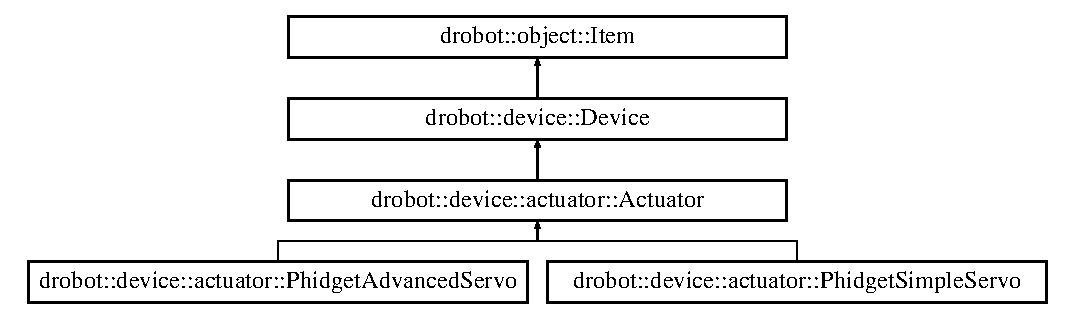
\includegraphics[height=3.835616cm]{classdrobot_1_1device_1_1actuator_1_1Actuator}
\end{center}
\end{figure}
\subsection*{Public Member Functions}
\begin{DoxyCompactItemize}
\item 
\hypertarget{classdrobot_1_1device_1_1actuator_1_1Actuator_ab13bc9a1bb826a403767e5af41558352}{{\bfseries Actuator} (std\-::string name)}\label{classdrobot_1_1device_1_1actuator_1_1Actuator_ab13bc9a1bb826a403767e5af41558352}

\item 
virtual double \hyperlink{classdrobot_1_1device_1_1actuator_1_1Actuator_aea525e325f2eb2058a37db3e014bb872}{get\-Position} ()=0
\item 
virtual void \hyperlink{classdrobot_1_1device_1_1actuator_1_1Actuator_a65fa025b3c0c69d81012454145c7ac69}{set\-Position} (double position)=0
\begin{DoxyCompactList}\small\item\em set motor position. The motor will always move to the last set position. \end{DoxyCompactList}\item 
virtual double \hyperlink{classdrobot_1_1device_1_1actuator_1_1Actuator_a7a4c195442470d46275f62446e5d2535}{get\-Position\-Min} ()=0
\item 
virtual double \hyperlink{classdrobot_1_1device_1_1actuator_1_1Actuator_a3a02ed0a72f8ab360748df0d9872eeb3}{get\-Position\-Max} ()=0
\item 
virtual double \hyperlink{classdrobot_1_1device_1_1actuator_1_1Actuator_a9fea4e618e465cbcc9a207740dbc5410}{get\-Velocity} ()=0
\item 
virtual void \hyperlink{classdrobot_1_1device_1_1actuator_1_1Actuator_a452a63a9cf5daf479c12b99c3e99679c}{set\-Velocity} (double velocity)=0
\begin{DoxyCompactList}\small\item\em set current velocity \end{DoxyCompactList}\item 
virtual double \hyperlink{classdrobot_1_1device_1_1actuator_1_1Actuator_a3ddbc25d10ca91b0719ad8b3b6220948}{get\-Velocity\-Min} ()=0
\item 
virtual double \hyperlink{classdrobot_1_1device_1_1actuator_1_1Actuator_a5a018f4e240fb1a483307c03a7662f3d}{get\-Velocity\-Max} ()=0
\item 
virtual double \hyperlink{classdrobot_1_1device_1_1actuator_1_1Actuator_a9dd6e74032417e5a84946925c655047c}{get\-Acceleration} ()=0
\item 
virtual void \hyperlink{classdrobot_1_1device_1_1actuator_1_1Actuator_a4056ed7c5038c86cd1ed24425a8e2d87}{set\-Acceleration} (double acceleration)=0
\begin{DoxyCompactList}\small\item\em set current acceleration \end{DoxyCompactList}\item 
virtual double \hyperlink{classdrobot_1_1device_1_1actuator_1_1Actuator_a16714b00aafdd84affaf9bc3a8383c48}{get\-Acceleration\-Min} ()=0
\item 
virtual double \hyperlink{classdrobot_1_1device_1_1actuator_1_1Actuator_a74e4fc92b8a3661ccbc44435411fbfca}{get\-Acceleration\-Max} ()=0
\end{DoxyCompactItemize}
\subsection*{Additional Inherited Members}


\subsection{Detailed Description}
Base class for all the actuators. 

\subsection{Member Function Documentation}
\hypertarget{classdrobot_1_1device_1_1actuator_1_1Actuator_a9dd6e74032417e5a84946925c655047c}{\index{drobot\-::device\-::actuator\-::\-Actuator@{drobot\-::device\-::actuator\-::\-Actuator}!get\-Acceleration@{get\-Acceleration}}
\index{get\-Acceleration@{get\-Acceleration}!drobot::device::actuator::Actuator@{drobot\-::device\-::actuator\-::\-Actuator}}
\subsubsection[{get\-Acceleration}]{\setlength{\rightskip}{0pt plus 5cm}virtual double drobot\-::device\-::actuator\-::\-Actuator\-::get\-Acceleration (
\begin{DoxyParamCaption}
{}
\end{DoxyParamCaption}
)\hspace{0.3cm}{\ttfamily [pure virtual]}}}\label{classdrobot_1_1device_1_1actuator_1_1Actuator_a9dd6e74032417e5a84946925c655047c}
\begin{DoxyReturn}{Returns}
current acceleration 
\end{DoxyReturn}


Implemented in \hyperlink{classdrobot_1_1device_1_1actuator_1_1PhidgetSimpleServo_ab9aee84e3e9b714298df2891f9bf9d89}{drobot\-::device\-::actuator\-::\-Phidget\-Simple\-Servo}, and \hyperlink{classdrobot_1_1device_1_1actuator_1_1PhidgetAdvancedServo_ae7fa5d92717bd981d753ef03b9c32da9}{drobot\-::device\-::actuator\-::\-Phidget\-Advanced\-Servo}.

\hypertarget{classdrobot_1_1device_1_1actuator_1_1Actuator_a74e4fc92b8a3661ccbc44435411fbfca}{\index{drobot\-::device\-::actuator\-::\-Actuator@{drobot\-::device\-::actuator\-::\-Actuator}!get\-Acceleration\-Max@{get\-Acceleration\-Max}}
\index{get\-Acceleration\-Max@{get\-Acceleration\-Max}!drobot::device::actuator::Actuator@{drobot\-::device\-::actuator\-::\-Actuator}}
\subsubsection[{get\-Acceleration\-Max}]{\setlength{\rightskip}{0pt plus 5cm}virtual double drobot\-::device\-::actuator\-::\-Actuator\-::get\-Acceleration\-Max (
\begin{DoxyParamCaption}
{}
\end{DoxyParamCaption}
)\hspace{0.3cm}{\ttfamily [pure virtual]}}}\label{classdrobot_1_1device_1_1actuator_1_1Actuator_a74e4fc92b8a3661ccbc44435411fbfca}
\begin{DoxyReturn}{Returns}
maximal possible acceleration 
\end{DoxyReturn}


Implemented in \hyperlink{classdrobot_1_1device_1_1actuator_1_1PhidgetSimpleServo_a33019d0481fe3e18179291c3090bb8aa}{drobot\-::device\-::actuator\-::\-Phidget\-Simple\-Servo}, and \hyperlink{classdrobot_1_1device_1_1actuator_1_1PhidgetAdvancedServo_a91960e941fe0813b402dbb214f41be2e}{drobot\-::device\-::actuator\-::\-Phidget\-Advanced\-Servo}.

\hypertarget{classdrobot_1_1device_1_1actuator_1_1Actuator_a16714b00aafdd84affaf9bc3a8383c48}{\index{drobot\-::device\-::actuator\-::\-Actuator@{drobot\-::device\-::actuator\-::\-Actuator}!get\-Acceleration\-Min@{get\-Acceleration\-Min}}
\index{get\-Acceleration\-Min@{get\-Acceleration\-Min}!drobot::device::actuator::Actuator@{drobot\-::device\-::actuator\-::\-Actuator}}
\subsubsection[{get\-Acceleration\-Min}]{\setlength{\rightskip}{0pt plus 5cm}virtual double drobot\-::device\-::actuator\-::\-Actuator\-::get\-Acceleration\-Min (
\begin{DoxyParamCaption}
{}
\end{DoxyParamCaption}
)\hspace{0.3cm}{\ttfamily [pure virtual]}}}\label{classdrobot_1_1device_1_1actuator_1_1Actuator_a16714b00aafdd84affaf9bc3a8383c48}
\begin{DoxyReturn}{Returns}
minimal possible acceleration 
\end{DoxyReturn}


Implemented in \hyperlink{classdrobot_1_1device_1_1actuator_1_1PhidgetSimpleServo_a76961c60cfa11ddae2588555eba8a223}{drobot\-::device\-::actuator\-::\-Phidget\-Simple\-Servo}, and \hyperlink{classdrobot_1_1device_1_1actuator_1_1PhidgetAdvancedServo_a5ff12831380c5ed0cd0ed131d0725f2b}{drobot\-::device\-::actuator\-::\-Phidget\-Advanced\-Servo}.

\hypertarget{classdrobot_1_1device_1_1actuator_1_1Actuator_aea525e325f2eb2058a37db3e014bb872}{\index{drobot\-::device\-::actuator\-::\-Actuator@{drobot\-::device\-::actuator\-::\-Actuator}!get\-Position@{get\-Position}}
\index{get\-Position@{get\-Position}!drobot::device::actuator::Actuator@{drobot\-::device\-::actuator\-::\-Actuator}}
\subsubsection[{get\-Position}]{\setlength{\rightskip}{0pt plus 5cm}virtual double drobot\-::device\-::actuator\-::\-Actuator\-::get\-Position (
\begin{DoxyParamCaption}
{}
\end{DoxyParamCaption}
)\hspace{0.3cm}{\ttfamily [pure virtual]}}}\label{classdrobot_1_1device_1_1actuator_1_1Actuator_aea525e325f2eb2058a37db3e014bb872}
\begin{DoxyReturn}{Returns}
current motor position 
\end{DoxyReturn}


Implemented in \hyperlink{classdrobot_1_1device_1_1actuator_1_1PhidgetSimpleServo_a4b63fb0ed00c9594037a53827b3bfdb5}{drobot\-::device\-::actuator\-::\-Phidget\-Simple\-Servo}, and \hyperlink{classdrobot_1_1device_1_1actuator_1_1PhidgetAdvancedServo_aa3661ee800d3f130322abcd125a103ee}{drobot\-::device\-::actuator\-::\-Phidget\-Advanced\-Servo}.

\hypertarget{classdrobot_1_1device_1_1actuator_1_1Actuator_a3a02ed0a72f8ab360748df0d9872eeb3}{\index{drobot\-::device\-::actuator\-::\-Actuator@{drobot\-::device\-::actuator\-::\-Actuator}!get\-Position\-Max@{get\-Position\-Max}}
\index{get\-Position\-Max@{get\-Position\-Max}!drobot::device::actuator::Actuator@{drobot\-::device\-::actuator\-::\-Actuator}}
\subsubsection[{get\-Position\-Max}]{\setlength{\rightskip}{0pt plus 5cm}virtual double drobot\-::device\-::actuator\-::\-Actuator\-::get\-Position\-Max (
\begin{DoxyParamCaption}
{}
\end{DoxyParamCaption}
)\hspace{0.3cm}{\ttfamily [pure virtual]}}}\label{classdrobot_1_1device_1_1actuator_1_1Actuator_a3a02ed0a72f8ab360748df0d9872eeb3}
\begin{DoxyReturn}{Returns}
minimal possible position 
\end{DoxyReturn}


Implemented in \hyperlink{classdrobot_1_1device_1_1actuator_1_1PhidgetSimpleServo_a6a0c6bc3edd91bc7cdcbb3ceb6e35499}{drobot\-::device\-::actuator\-::\-Phidget\-Simple\-Servo}, and \hyperlink{classdrobot_1_1device_1_1actuator_1_1PhidgetAdvancedServo_a12335ab5360aa850bbc0a3b52028d62a}{drobot\-::device\-::actuator\-::\-Phidget\-Advanced\-Servo}.

\hypertarget{classdrobot_1_1device_1_1actuator_1_1Actuator_a7a4c195442470d46275f62446e5d2535}{\index{drobot\-::device\-::actuator\-::\-Actuator@{drobot\-::device\-::actuator\-::\-Actuator}!get\-Position\-Min@{get\-Position\-Min}}
\index{get\-Position\-Min@{get\-Position\-Min}!drobot::device::actuator::Actuator@{drobot\-::device\-::actuator\-::\-Actuator}}
\subsubsection[{get\-Position\-Min}]{\setlength{\rightskip}{0pt plus 5cm}virtual double drobot\-::device\-::actuator\-::\-Actuator\-::get\-Position\-Min (
\begin{DoxyParamCaption}
{}
\end{DoxyParamCaption}
)\hspace{0.3cm}{\ttfamily [pure virtual]}}}\label{classdrobot_1_1device_1_1actuator_1_1Actuator_a7a4c195442470d46275f62446e5d2535}
\begin{DoxyReturn}{Returns}
maximal possible position 
\end{DoxyReturn}


Implemented in \hyperlink{classdrobot_1_1device_1_1actuator_1_1PhidgetSimpleServo_a37cbebc54653841ec66e3176a3e46241}{drobot\-::device\-::actuator\-::\-Phidget\-Simple\-Servo}, and \hyperlink{classdrobot_1_1device_1_1actuator_1_1PhidgetAdvancedServo_afd48104555df3fa2a8750eb19c118417}{drobot\-::device\-::actuator\-::\-Phidget\-Advanced\-Servo}.

\hypertarget{classdrobot_1_1device_1_1actuator_1_1Actuator_a9fea4e618e465cbcc9a207740dbc5410}{\index{drobot\-::device\-::actuator\-::\-Actuator@{drobot\-::device\-::actuator\-::\-Actuator}!get\-Velocity@{get\-Velocity}}
\index{get\-Velocity@{get\-Velocity}!drobot::device::actuator::Actuator@{drobot\-::device\-::actuator\-::\-Actuator}}
\subsubsection[{get\-Velocity}]{\setlength{\rightskip}{0pt plus 5cm}virtual double drobot\-::device\-::actuator\-::\-Actuator\-::get\-Velocity (
\begin{DoxyParamCaption}
{}
\end{DoxyParamCaption}
)\hspace{0.3cm}{\ttfamily [pure virtual]}}}\label{classdrobot_1_1device_1_1actuator_1_1Actuator_a9fea4e618e465cbcc9a207740dbc5410}
\begin{DoxyReturn}{Returns}
current velocity 
\end{DoxyReturn}


Implemented in \hyperlink{classdrobot_1_1device_1_1actuator_1_1PhidgetAdvancedServo_ade608d8b4b469ae3203fcf968f3b1455}{drobot\-::device\-::actuator\-::\-Phidget\-Advanced\-Servo}, and \hyperlink{classdrobot_1_1device_1_1actuator_1_1PhidgetSimpleServo_ac95f8be440b0fbed1c9d33b2d919d804}{drobot\-::device\-::actuator\-::\-Phidget\-Simple\-Servo}.

\hypertarget{classdrobot_1_1device_1_1actuator_1_1Actuator_a5a018f4e240fb1a483307c03a7662f3d}{\index{drobot\-::device\-::actuator\-::\-Actuator@{drobot\-::device\-::actuator\-::\-Actuator}!get\-Velocity\-Max@{get\-Velocity\-Max}}
\index{get\-Velocity\-Max@{get\-Velocity\-Max}!drobot::device::actuator::Actuator@{drobot\-::device\-::actuator\-::\-Actuator}}
\subsubsection[{get\-Velocity\-Max}]{\setlength{\rightskip}{0pt plus 5cm}virtual double drobot\-::device\-::actuator\-::\-Actuator\-::get\-Velocity\-Max (
\begin{DoxyParamCaption}
{}
\end{DoxyParamCaption}
)\hspace{0.3cm}{\ttfamily [pure virtual]}}}\label{classdrobot_1_1device_1_1actuator_1_1Actuator_a5a018f4e240fb1a483307c03a7662f3d}
\begin{DoxyReturn}{Returns}
maximal possible velocity 
\end{DoxyReturn}


Implemented in \hyperlink{classdrobot_1_1device_1_1actuator_1_1PhidgetAdvancedServo_a9a0090b6dcdb7dd022687665f4ca9dd9}{drobot\-::device\-::actuator\-::\-Phidget\-Advanced\-Servo}, and \hyperlink{classdrobot_1_1device_1_1actuator_1_1PhidgetSimpleServo_aa54b52796cfb651db75b762dc319b38f}{drobot\-::device\-::actuator\-::\-Phidget\-Simple\-Servo}.

\hypertarget{classdrobot_1_1device_1_1actuator_1_1Actuator_a3ddbc25d10ca91b0719ad8b3b6220948}{\index{drobot\-::device\-::actuator\-::\-Actuator@{drobot\-::device\-::actuator\-::\-Actuator}!get\-Velocity\-Min@{get\-Velocity\-Min}}
\index{get\-Velocity\-Min@{get\-Velocity\-Min}!drobot::device::actuator::Actuator@{drobot\-::device\-::actuator\-::\-Actuator}}
\subsubsection[{get\-Velocity\-Min}]{\setlength{\rightskip}{0pt plus 5cm}virtual double drobot\-::device\-::actuator\-::\-Actuator\-::get\-Velocity\-Min (
\begin{DoxyParamCaption}
{}
\end{DoxyParamCaption}
)\hspace{0.3cm}{\ttfamily [pure virtual]}}}\label{classdrobot_1_1device_1_1actuator_1_1Actuator_a3ddbc25d10ca91b0719ad8b3b6220948}
\begin{DoxyReturn}{Returns}
minimal possible velocity 
\end{DoxyReturn}


Implemented in \hyperlink{classdrobot_1_1device_1_1actuator_1_1PhidgetAdvancedServo_a77b7e687934b58aec83d19c62071bf69}{drobot\-::device\-::actuator\-::\-Phidget\-Advanced\-Servo}, and \hyperlink{classdrobot_1_1device_1_1actuator_1_1PhidgetSimpleServo_a9880f9f9f0cd83abc3b8d927316ed843}{drobot\-::device\-::actuator\-::\-Phidget\-Simple\-Servo}.

\hypertarget{classdrobot_1_1device_1_1actuator_1_1Actuator_a4056ed7c5038c86cd1ed24425a8e2d87}{\index{drobot\-::device\-::actuator\-::\-Actuator@{drobot\-::device\-::actuator\-::\-Actuator}!set\-Acceleration@{set\-Acceleration}}
\index{set\-Acceleration@{set\-Acceleration}!drobot::device::actuator::Actuator@{drobot\-::device\-::actuator\-::\-Actuator}}
\subsubsection[{set\-Acceleration}]{\setlength{\rightskip}{0pt plus 5cm}virtual void drobot\-::device\-::actuator\-::\-Actuator\-::set\-Acceleration (
\begin{DoxyParamCaption}
\item[{double}]{acceleration}
\end{DoxyParamCaption}
)\hspace{0.3cm}{\ttfamily [pure virtual]}}}\label{classdrobot_1_1device_1_1actuator_1_1Actuator_a4056ed7c5038c86cd1ed24425a8e2d87}


set current acceleration 


\begin{DoxyParams}{Parameters}
{\em acceleration} & \\
\hline
\end{DoxyParams}


Implemented in \hyperlink{classdrobot_1_1device_1_1actuator_1_1PhidgetSimpleServo_a9577403e844e3d18f66fd23c2bdf1e8f}{drobot\-::device\-::actuator\-::\-Phidget\-Simple\-Servo}, and \hyperlink{classdrobot_1_1device_1_1actuator_1_1PhidgetAdvancedServo_a7c1d34496318852e20f81b145584c852}{drobot\-::device\-::actuator\-::\-Phidget\-Advanced\-Servo}.

\hypertarget{classdrobot_1_1device_1_1actuator_1_1Actuator_a65fa025b3c0c69d81012454145c7ac69}{\index{drobot\-::device\-::actuator\-::\-Actuator@{drobot\-::device\-::actuator\-::\-Actuator}!set\-Position@{set\-Position}}
\index{set\-Position@{set\-Position}!drobot::device::actuator::Actuator@{drobot\-::device\-::actuator\-::\-Actuator}}
\subsubsection[{set\-Position}]{\setlength{\rightskip}{0pt plus 5cm}virtual void drobot\-::device\-::actuator\-::\-Actuator\-::set\-Position (
\begin{DoxyParamCaption}
\item[{double}]{position}
\end{DoxyParamCaption}
)\hspace{0.3cm}{\ttfamily [pure virtual]}}}\label{classdrobot_1_1device_1_1actuator_1_1Actuator_a65fa025b3c0c69d81012454145c7ac69}


set motor position. The motor will always move to the last set position. 


\begin{DoxyParams}{Parameters}
{\em position} & \\
\hline
\end{DoxyParams}


Implemented in \hyperlink{classdrobot_1_1device_1_1actuator_1_1PhidgetSimpleServo_a9c08fb8a75bded49f53635d9184ce9e2}{drobot\-::device\-::actuator\-::\-Phidget\-Simple\-Servo}, and \hyperlink{classdrobot_1_1device_1_1actuator_1_1PhidgetAdvancedServo_a97cf6ba7524e113eeaa8bbe44ff3058a}{drobot\-::device\-::actuator\-::\-Phidget\-Advanced\-Servo}.

\hypertarget{classdrobot_1_1device_1_1actuator_1_1Actuator_a452a63a9cf5daf479c12b99c3e99679c}{\index{drobot\-::device\-::actuator\-::\-Actuator@{drobot\-::device\-::actuator\-::\-Actuator}!set\-Velocity@{set\-Velocity}}
\index{set\-Velocity@{set\-Velocity}!drobot::device::actuator::Actuator@{drobot\-::device\-::actuator\-::\-Actuator}}
\subsubsection[{set\-Velocity}]{\setlength{\rightskip}{0pt plus 5cm}virtual void drobot\-::device\-::actuator\-::\-Actuator\-::set\-Velocity (
\begin{DoxyParamCaption}
\item[{double}]{velocity}
\end{DoxyParamCaption}
)\hspace{0.3cm}{\ttfamily [pure virtual]}}}\label{classdrobot_1_1device_1_1actuator_1_1Actuator_a452a63a9cf5daf479c12b99c3e99679c}


set current velocity 


\begin{DoxyParams}{Parameters}
{\em velocity} & \\
\hline
\end{DoxyParams}


Implemented in \hyperlink{classdrobot_1_1device_1_1actuator_1_1PhidgetAdvancedServo_ae960026b28343c37bf163bd7c0f84e4b}{drobot\-::device\-::actuator\-::\-Phidget\-Advanced\-Servo}, and \hyperlink{classdrobot_1_1device_1_1actuator_1_1PhidgetSimpleServo_af0c80a2d8cacc535b7b529eb84fc1075}{drobot\-::device\-::actuator\-::\-Phidget\-Simple\-Servo}.



The documentation for this class was generated from the following files\-:\begin{DoxyCompactItemize}
\item 
src/drobot/device/actuator/actuator.\-h\item 
src/drobot/device/actuator/actuator.\-cpp\end{DoxyCompactItemize}

\hypertarget{classdrobot_1_1device_1_1actuator_1_1channel_1_1ActuatorAccelerationChannel}{\section{drobot\-:\-:device\-:\-:actuator\-:\-:channel\-:\-:Actuator\-Acceleration\-Channel Class Reference}
\label{classdrobot_1_1device_1_1actuator_1_1channel_1_1ActuatorAccelerationChannel}\index{drobot\-::device\-::actuator\-::channel\-::\-Actuator\-Acceleration\-Channel@{drobot\-::device\-::actuator\-::channel\-::\-Actuator\-Acceleration\-Channel}}
}
Inheritance diagram for drobot\-:\-:device\-:\-:actuator\-:\-:channel\-:\-:Actuator\-Acceleration\-Channel\-:\begin{figure}[H]
\begin{center}
\leavevmode
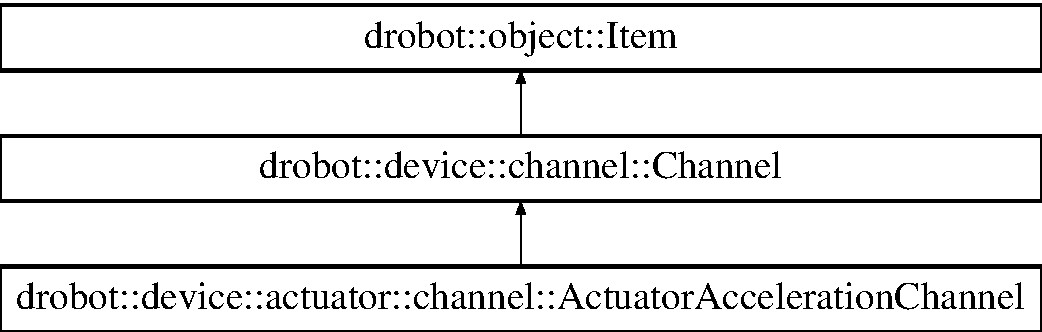
\includegraphics[height=3.000000cm]{classdrobot_1_1device_1_1actuator_1_1channel_1_1ActuatorAccelerationChannel}
\end{center}
\end{figure}
\subsection*{Public Member Functions}
\begin{DoxyCompactItemize}
\item 
\hypertarget{classdrobot_1_1device_1_1actuator_1_1channel_1_1ActuatorAccelerationChannel_a047d46d5d7695c45d6ba282a1fe50ec5}{{\bfseries Actuator\-Acceleration\-Channel} (std\-::string name, device\-::channel\-::\-Channel\-Type type)}\label{classdrobot_1_1device_1_1actuator_1_1channel_1_1ActuatorAccelerationChannel_a047d46d5d7695c45d6ba282a1fe50ec5}

\item 
\hypertarget{classdrobot_1_1device_1_1actuator_1_1channel_1_1ActuatorAccelerationChannel_a99382509919e221b7623ab632736a19d}{{\bfseries Actuator\-Acceleration\-Channel} (std\-::string name, device\-::channel\-::\-Channel\-Type type, \hyperlink{classdrobot_1_1device_1_1channel_1_1Normalizer}{device\-::channel\-::\-Normalizer} $\ast$normalizer, \hyperlink{classdrobot_1_1device_1_1Device}{device\-::\-Device} $\ast$device)}\label{classdrobot_1_1device_1_1actuator_1_1channel_1_1ActuatorAccelerationChannel_a99382509919e221b7623ab632736a19d}

\end{DoxyCompactItemize}
\subsection*{Protected Member Functions}
\begin{DoxyCompactItemize}
\item 
virtual void \hyperlink{classdrobot_1_1device_1_1actuator_1_1channel_1_1ActuatorAccelerationChannel_a33cdc24b62518961f8c003a31097c48d}{set\-Value} (double value)
\begin{DoxyCompactList}\small\item\em sets the value directly to the device \end{DoxyCompactList}\item 
virtual double \hyperlink{classdrobot_1_1device_1_1actuator_1_1channel_1_1ActuatorAccelerationChannel_a8dab242bd8099a88a2fd981508827224}{get\-Value} ()
\begin{DoxyCompactList}\small\item\em returns the value directly from the device. \end{DoxyCompactList}\end{DoxyCompactItemize}
\subsection*{Additional Inherited Members}


\subsection{Member Function Documentation}
\hypertarget{classdrobot_1_1device_1_1actuator_1_1channel_1_1ActuatorAccelerationChannel_a8dab242bd8099a88a2fd981508827224}{\index{drobot\-::device\-::actuator\-::channel\-::\-Actuator\-Acceleration\-Channel@{drobot\-::device\-::actuator\-::channel\-::\-Actuator\-Acceleration\-Channel}!get\-Value@{get\-Value}}
\index{get\-Value@{get\-Value}!drobot::device::actuator::channel::ActuatorAccelerationChannel@{drobot\-::device\-::actuator\-::channel\-::\-Actuator\-Acceleration\-Channel}}
\subsubsection[{get\-Value}]{\setlength{\rightskip}{0pt plus 5cm}double drobot\-::device\-::actuator\-::channel\-::\-Actuator\-Acceleration\-Channel\-::get\-Value (
\begin{DoxyParamCaption}
{}
\end{DoxyParamCaption}
)\hspace{0.3cm}{\ttfamily [protected]}, {\ttfamily [virtual]}}}\label{classdrobot_1_1device_1_1actuator_1_1channel_1_1ActuatorAccelerationChannel_a8dab242bd8099a88a2fd981508827224}


returns the value directly from the device. 

\begin{DoxyReturn}{Returns}

\end{DoxyReturn}


Implements \hyperlink{classdrobot_1_1device_1_1channel_1_1Channel_a42f0978ebb99d13a89c1785baf69a4d8}{drobot\-::device\-::channel\-::\-Channel}.

\hypertarget{classdrobot_1_1device_1_1actuator_1_1channel_1_1ActuatorAccelerationChannel_a33cdc24b62518961f8c003a31097c48d}{\index{drobot\-::device\-::actuator\-::channel\-::\-Actuator\-Acceleration\-Channel@{drobot\-::device\-::actuator\-::channel\-::\-Actuator\-Acceleration\-Channel}!set\-Value@{set\-Value}}
\index{set\-Value@{set\-Value}!drobot::device::actuator::channel::ActuatorAccelerationChannel@{drobot\-::device\-::actuator\-::channel\-::\-Actuator\-Acceleration\-Channel}}
\subsubsection[{set\-Value}]{\setlength{\rightskip}{0pt plus 5cm}void drobot\-::device\-::actuator\-::channel\-::\-Actuator\-Acceleration\-Channel\-::set\-Value (
\begin{DoxyParamCaption}
\item[{double}]{value}
\end{DoxyParamCaption}
)\hspace{0.3cm}{\ttfamily [protected]}, {\ttfamily [virtual]}}}\label{classdrobot_1_1device_1_1actuator_1_1channel_1_1ActuatorAccelerationChannel_a33cdc24b62518961f8c003a31097c48d}


sets the value directly to the device 


\begin{DoxyParams}{Parameters}
{\em value} & \\
\hline
\end{DoxyParams}


Implements \hyperlink{classdrobot_1_1device_1_1channel_1_1Channel_a612a3f6afe59e238583d6d40d9ddcaf8}{drobot\-::device\-::channel\-::\-Channel}.



The documentation for this class was generated from the following files\-:\begin{DoxyCompactItemize}
\item 
src/drobot/device/actuator/channel/actuatoraccelerationchannel.\-h\item 
src/drobot/device/actuator/channel/actuatoraccelerationchannel.\-cpp\end{DoxyCompactItemize}

\hypertarget{classdrobot_1_1device_1_1actuator_1_1channel_1_1ActuatorAccelerationChannelFactory}{\section{drobot\-:\-:device\-:\-:actuator\-:\-:channel\-:\-:Actuator\-Acceleration\-Channel\-Factory Class Reference}
\label{classdrobot_1_1device_1_1actuator_1_1channel_1_1ActuatorAccelerationChannelFactory}\index{drobot\-::device\-::actuator\-::channel\-::\-Actuator\-Acceleration\-Channel\-Factory@{drobot\-::device\-::actuator\-::channel\-::\-Actuator\-Acceleration\-Channel\-Factory}}
}
Inheritance diagram for drobot\-:\-:device\-:\-:actuator\-:\-:channel\-:\-:Actuator\-Acceleration\-Channel\-Factory\-:\begin{figure}[H]
\begin{center}
\leavevmode
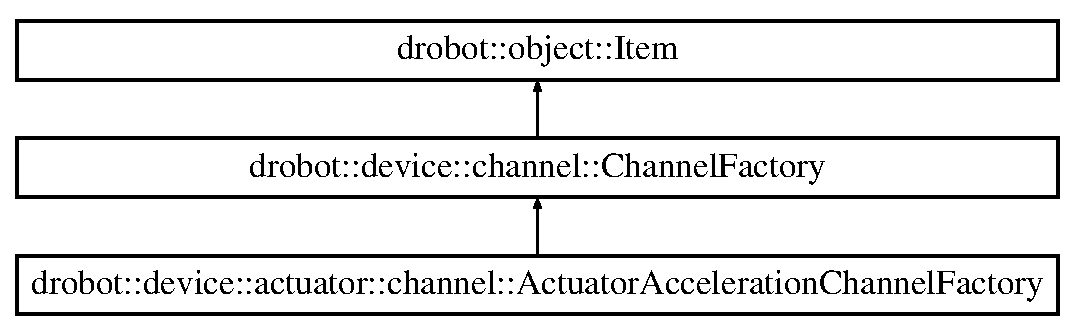
\includegraphics[height=3.000000cm]{classdrobot_1_1device_1_1actuator_1_1channel_1_1ActuatorAccelerationChannelFactory}
\end{center}
\end{figure}
\subsection*{Public Member Functions}
\begin{DoxyCompactItemize}
\item 
virtual void \hyperlink{classdrobot_1_1device_1_1actuator_1_1channel_1_1ActuatorAccelerationChannelFactory_a077744d3866b134b15cfe9522eeb99e3}{create\-From\-Dom\-Element} (Q\-Dom\-Element element, \hyperlink{classdrobot_1_1device_1_1Device}{Device} $\ast$device)
\begin{DoxyCompactList}\small\item\em create channel from Dom Tree element \end{DoxyCompactList}\end{DoxyCompactItemize}
\subsection*{Additional Inherited Members}


\subsection{Member Function Documentation}
\hypertarget{classdrobot_1_1device_1_1actuator_1_1channel_1_1ActuatorAccelerationChannelFactory_a077744d3866b134b15cfe9522eeb99e3}{\index{drobot\-::device\-::actuator\-::channel\-::\-Actuator\-Acceleration\-Channel\-Factory@{drobot\-::device\-::actuator\-::channel\-::\-Actuator\-Acceleration\-Channel\-Factory}!create\-From\-Dom\-Element@{create\-From\-Dom\-Element}}
\index{create\-From\-Dom\-Element@{create\-From\-Dom\-Element}!drobot::device::actuator::channel::ActuatorAccelerationChannelFactory@{drobot\-::device\-::actuator\-::channel\-::\-Actuator\-Acceleration\-Channel\-Factory}}
\subsubsection[{create\-From\-Dom\-Element}]{\setlength{\rightskip}{0pt plus 5cm}void drobot\-::device\-::actuator\-::channel\-::\-Actuator\-Acceleration\-Channel\-Factory\-::create\-From\-Dom\-Element (
\begin{DoxyParamCaption}
\item[{Q\-Dom\-Element}]{element, }
\item[{{\bf Device} $\ast$}]{device}
\end{DoxyParamCaption}
)\hspace{0.3cm}{\ttfamily [virtual]}}}\label{classdrobot_1_1device_1_1actuator_1_1channel_1_1ActuatorAccelerationChannelFactory_a077744d3866b134b15cfe9522eeb99e3}


create channel from Dom Tree element 

this method has to create one or more channels from the element and add it to the device. 
\begin{DoxyParams}{Parameters}
{\em element} & \\
\hline
{\em device} & \\
\hline
\end{DoxyParams}


Implements \hyperlink{classdrobot_1_1device_1_1channel_1_1ChannelFactory_ab59ee44782347b8878a471bf87f06c43}{drobot\-::device\-::channel\-::\-Channel\-Factory}.



The documentation for this class was generated from the following files\-:\begin{DoxyCompactItemize}
\item 
/home/imanol/workspace/drobot/new/src/drobot/device/actuator/channel/actuatoraccelerationchannelfactory.\-h\item 
/home/imanol/workspace/drobot/new/src/drobot/device/actuator/channel/actuatoraccelerationchannelfactory.\-cpp\end{DoxyCompactItemize}

\hypertarget{classdrobot_1_1device_1_1actuator_1_1ActuatorBoard}{\section{drobot\-:\-:device\-:\-:actuator\-:\-:Actuator\-Board Class Reference}
\label{classdrobot_1_1device_1_1actuator_1_1ActuatorBoard}\index{drobot\-::device\-::actuator\-::\-Actuator\-Board@{drobot\-::device\-::actuator\-::\-Actuator\-Board}}
}


Baseclass for all the actuator boards.  




{\ttfamily \#include $<$actuatorboard.\-h$>$}

Inheritance diagram for drobot\-:\-:device\-:\-:actuator\-:\-:Actuator\-Board\-:\begin{figure}[H]
\begin{center}
\leavevmode
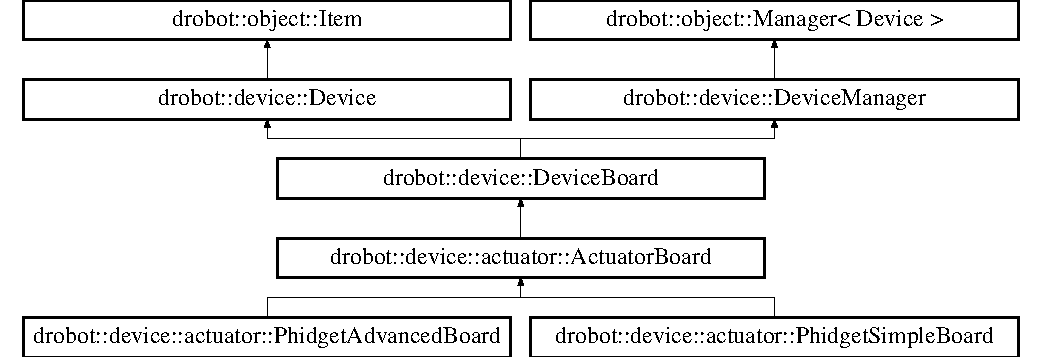
\includegraphics[height=4.794520cm]{classdrobot_1_1device_1_1actuator_1_1ActuatorBoard}
\end{center}
\end{figure}
\subsection*{Public Member Functions}
\begin{DoxyCompactItemize}
\item 
\hypertarget{classdrobot_1_1device_1_1actuator_1_1ActuatorBoard_aa869681bee8e71c28b531457d0ba057c}{{\bfseries Actuator\-Board} (std\-::string name)}\label{classdrobot_1_1device_1_1actuator_1_1ActuatorBoard_aa869681bee8e71c28b531457d0ba057c}

\item 
\hypertarget{classdrobot_1_1device_1_1actuator_1_1ActuatorBoard_ac76eda87a74d2701c9ce686ccc2b5932}{std\-::vector$<$ \hyperlink{classdrobot_1_1device_1_1actuator_1_1Actuator}{Actuator} $\ast$ $>$ {\bfseries get\-Actuators} ()}\label{classdrobot_1_1device_1_1actuator_1_1ActuatorBoard_ac76eda87a74d2701c9ce686ccc2b5932}

\item 
\hypertarget{classdrobot_1_1device_1_1actuator_1_1ActuatorBoard_a5cb7e13fef66d8aef30ad8ea1d509dcd}{\hyperlink{classdrobot_1_1device_1_1actuator_1_1Actuator}{Actuator} $\ast$ {\bfseries get\-Actuator} (std\-::string name)}\label{classdrobot_1_1device_1_1actuator_1_1ActuatorBoard_a5cb7e13fef66d8aef30ad8ea1d509dcd}

\end{DoxyCompactItemize}
\subsection*{Additional Inherited Members}


\subsection{Detailed Description}
Baseclass for all the actuator boards. 

The documentation for this class was generated from the following files\-:\begin{DoxyCompactItemize}
\item 
/home/imanol/workspace/drobot/new/src/drobot/device/actuator/actuatorboard.\-h\item 
/home/imanol/workspace/drobot/new/src/drobot/device/actuator/actuatorboard.\-cpp\end{DoxyCompactItemize}

\hypertarget{classdrobot_1_1device_1_1actuator_1_1channel_1_1ActuatorPositionChannel}{\section{drobot\-:\-:device\-:\-:actuator\-:\-:channel\-:\-:Actuator\-Position\-Channel Class Reference}
\label{classdrobot_1_1device_1_1actuator_1_1channel_1_1ActuatorPositionChannel}\index{drobot\-::device\-::actuator\-::channel\-::\-Actuator\-Position\-Channel@{drobot\-::device\-::actuator\-::channel\-::\-Actuator\-Position\-Channel}}
}
Inheritance diagram for drobot\-:\-:device\-:\-:actuator\-:\-:channel\-:\-:Actuator\-Position\-Channel\-:\begin{figure}[H]
\begin{center}
\leavevmode
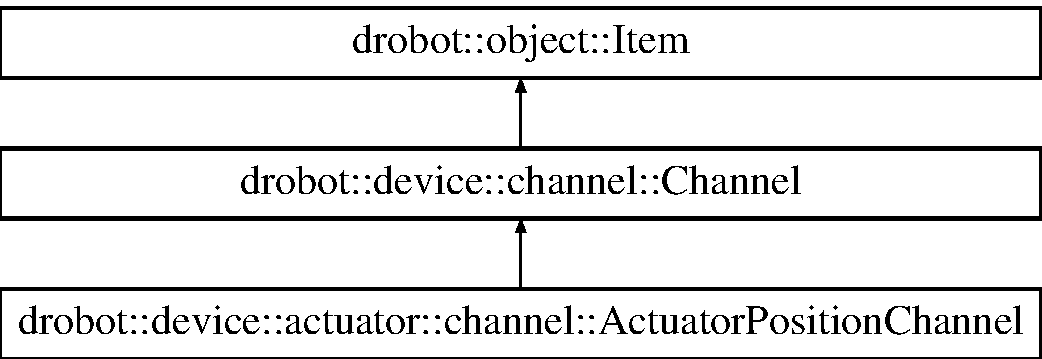
\includegraphics[height=3.000000cm]{classdrobot_1_1device_1_1actuator_1_1channel_1_1ActuatorPositionChannel}
\end{center}
\end{figure}
\subsection*{Public Member Functions}
\begin{DoxyCompactItemize}
\item 
\hypertarget{classdrobot_1_1device_1_1actuator_1_1channel_1_1ActuatorPositionChannel_a4ccdc5fa689006173ca5bb0aaf9c52a8}{{\bfseries Actuator\-Position\-Channel} (std\-::string name, device\-::channel\-::\-Channel\-Type type)}\label{classdrobot_1_1device_1_1actuator_1_1channel_1_1ActuatorPositionChannel_a4ccdc5fa689006173ca5bb0aaf9c52a8}

\item 
\hypertarget{classdrobot_1_1device_1_1actuator_1_1channel_1_1ActuatorPositionChannel_a89d497876bbb34d206cb88afeb462a20}{{\bfseries Actuator\-Position\-Channel} (std\-::string name, device\-::channel\-::\-Channel\-Type type, \hyperlink{classdrobot_1_1device_1_1channel_1_1Normalizer}{device\-::channel\-::\-Normalizer} $\ast$normalizer, \hyperlink{classdrobot_1_1device_1_1Device}{device\-::\-Device} $\ast$device)}\label{classdrobot_1_1device_1_1actuator_1_1channel_1_1ActuatorPositionChannel_a89d497876bbb34d206cb88afeb462a20}

\end{DoxyCompactItemize}
\subsection*{Protected Member Functions}
\begin{DoxyCompactItemize}
\item 
virtual void \hyperlink{classdrobot_1_1device_1_1actuator_1_1channel_1_1ActuatorPositionChannel_ac293318a0e51a0cca153326efd08d7c8}{set\-Value} (double value)
\begin{DoxyCompactList}\small\item\em sets the value directly to the device \end{DoxyCompactList}\item 
virtual double \hyperlink{classdrobot_1_1device_1_1actuator_1_1channel_1_1ActuatorPositionChannel_a21dd5208fd7d5c439d711871cfbbea9a}{get\-Value} ()
\begin{DoxyCompactList}\small\item\em returns the value directly from the device. \end{DoxyCompactList}\end{DoxyCompactItemize}
\subsection*{Additional Inherited Members}


\subsection{Member Function Documentation}
\hypertarget{classdrobot_1_1device_1_1actuator_1_1channel_1_1ActuatorPositionChannel_a21dd5208fd7d5c439d711871cfbbea9a}{\index{drobot\-::device\-::actuator\-::channel\-::\-Actuator\-Position\-Channel@{drobot\-::device\-::actuator\-::channel\-::\-Actuator\-Position\-Channel}!get\-Value@{get\-Value}}
\index{get\-Value@{get\-Value}!drobot::device::actuator::channel::ActuatorPositionChannel@{drobot\-::device\-::actuator\-::channel\-::\-Actuator\-Position\-Channel}}
\subsubsection[{get\-Value}]{\setlength{\rightskip}{0pt plus 5cm}double drobot\-::device\-::actuator\-::channel\-::\-Actuator\-Position\-Channel\-::get\-Value (
\begin{DoxyParamCaption}
{}
\end{DoxyParamCaption}
)\hspace{0.3cm}{\ttfamily [protected]}, {\ttfamily [virtual]}}}\label{classdrobot_1_1device_1_1actuator_1_1channel_1_1ActuatorPositionChannel_a21dd5208fd7d5c439d711871cfbbea9a}


returns the value directly from the device. 

\begin{DoxyReturn}{Returns}

\end{DoxyReturn}


Implements \hyperlink{classdrobot_1_1device_1_1channel_1_1Channel_a42f0978ebb99d13a89c1785baf69a4d8}{drobot\-::device\-::channel\-::\-Channel}.

\hypertarget{classdrobot_1_1device_1_1actuator_1_1channel_1_1ActuatorPositionChannel_ac293318a0e51a0cca153326efd08d7c8}{\index{drobot\-::device\-::actuator\-::channel\-::\-Actuator\-Position\-Channel@{drobot\-::device\-::actuator\-::channel\-::\-Actuator\-Position\-Channel}!set\-Value@{set\-Value}}
\index{set\-Value@{set\-Value}!drobot::device::actuator::channel::ActuatorPositionChannel@{drobot\-::device\-::actuator\-::channel\-::\-Actuator\-Position\-Channel}}
\subsubsection[{set\-Value}]{\setlength{\rightskip}{0pt plus 5cm}void drobot\-::device\-::actuator\-::channel\-::\-Actuator\-Position\-Channel\-::set\-Value (
\begin{DoxyParamCaption}
\item[{double}]{value}
\end{DoxyParamCaption}
)\hspace{0.3cm}{\ttfamily [protected]}, {\ttfamily [virtual]}}}\label{classdrobot_1_1device_1_1actuator_1_1channel_1_1ActuatorPositionChannel_ac293318a0e51a0cca153326efd08d7c8}


sets the value directly to the device 


\begin{DoxyParams}{Parameters}
{\em value} & \\
\hline
\end{DoxyParams}


Implements \hyperlink{classdrobot_1_1device_1_1channel_1_1Channel_a612a3f6afe59e238583d6d40d9ddcaf8}{drobot\-::device\-::channel\-::\-Channel}.



The documentation for this class was generated from the following files\-:\begin{DoxyCompactItemize}
\item 
src/drobot/device/actuator/channel/actuatorpositionchannel.\-h\item 
src/drobot/device/actuator/channel/actuatorpositionchannel.\-cpp\end{DoxyCompactItemize}

\hypertarget{classdrobot_1_1device_1_1actuator_1_1channel_1_1ActuatorPositionChannelFactory}{\section{drobot\-:\-:device\-:\-:actuator\-:\-:channel\-:\-:Actuator\-Position\-Channel\-Factory Class Reference}
\label{classdrobot_1_1device_1_1actuator_1_1channel_1_1ActuatorPositionChannelFactory}\index{drobot\-::device\-::actuator\-::channel\-::\-Actuator\-Position\-Channel\-Factory@{drobot\-::device\-::actuator\-::channel\-::\-Actuator\-Position\-Channel\-Factory}}
}
Inheritance diagram for drobot\-:\-:device\-:\-:actuator\-:\-:channel\-:\-:Actuator\-Position\-Channel\-Factory\-:\begin{figure}[H]
\begin{center}
\leavevmode
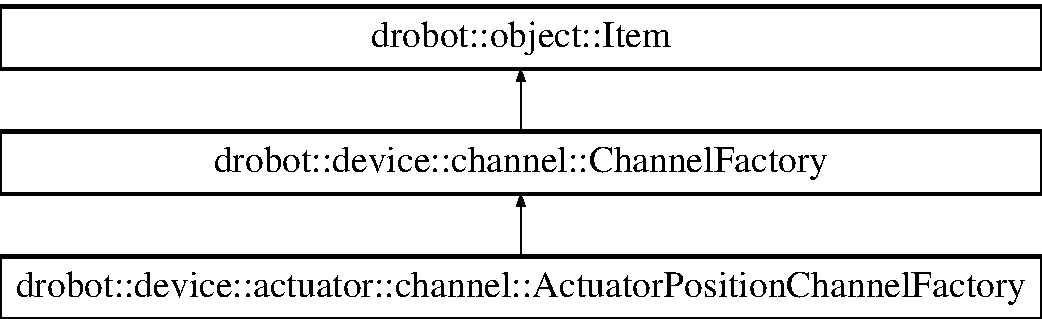
\includegraphics[height=3.000000cm]{classdrobot_1_1device_1_1actuator_1_1channel_1_1ActuatorPositionChannelFactory}
\end{center}
\end{figure}
\subsection*{Public Member Functions}
\begin{DoxyCompactItemize}
\item 
virtual void \hyperlink{classdrobot_1_1device_1_1actuator_1_1channel_1_1ActuatorPositionChannelFactory_a66d52953c14b0686b3dd61b9f8462476}{create\-From\-Dom\-Element} (Q\-Dom\-Element element, \hyperlink{classdrobot_1_1device_1_1Device}{Device} $\ast$device)
\begin{DoxyCompactList}\small\item\em create channel from Dom Tree element \end{DoxyCompactList}\end{DoxyCompactItemize}
\subsection*{Additional Inherited Members}


\subsection{Member Function Documentation}
\hypertarget{classdrobot_1_1device_1_1actuator_1_1channel_1_1ActuatorPositionChannelFactory_a66d52953c14b0686b3dd61b9f8462476}{\index{drobot\-::device\-::actuator\-::channel\-::\-Actuator\-Position\-Channel\-Factory@{drobot\-::device\-::actuator\-::channel\-::\-Actuator\-Position\-Channel\-Factory}!create\-From\-Dom\-Element@{create\-From\-Dom\-Element}}
\index{create\-From\-Dom\-Element@{create\-From\-Dom\-Element}!drobot::device::actuator::channel::ActuatorPositionChannelFactory@{drobot\-::device\-::actuator\-::channel\-::\-Actuator\-Position\-Channel\-Factory}}
\subsubsection[{create\-From\-Dom\-Element}]{\setlength{\rightskip}{0pt plus 5cm}void drobot\-::device\-::actuator\-::channel\-::\-Actuator\-Position\-Channel\-Factory\-::create\-From\-Dom\-Element (
\begin{DoxyParamCaption}
\item[{Q\-Dom\-Element}]{element, }
\item[{{\bf Device} $\ast$}]{device}
\end{DoxyParamCaption}
)\hspace{0.3cm}{\ttfamily [virtual]}}}\label{classdrobot_1_1device_1_1actuator_1_1channel_1_1ActuatorPositionChannelFactory_a66d52953c14b0686b3dd61b9f8462476}


create channel from Dom Tree element 

this method has to create one or more channels from the element and add it to the device. 
\begin{DoxyParams}{Parameters}
{\em element} & \\
\hline
{\em device} & \\
\hline
\end{DoxyParams}


Implements \hyperlink{classdrobot_1_1device_1_1channel_1_1ChannelFactory_ab59ee44782347b8878a471bf87f06c43}{drobot\-::device\-::channel\-::\-Channel\-Factory}.



The documentation for this class was generated from the following files\-:\begin{DoxyCompactItemize}
\item 
/home/imanol/workspace/drobot/new/src/drobot/device/actuator/channel/actuatorpositionchannelfactory.\-h\item 
/home/imanol/workspace/drobot/new/src/drobot/device/actuator/channel/actuatorpositionchannelfactory.\-cpp\end{DoxyCompactItemize}

\hypertarget{classdrobot_1_1device_1_1actuator_1_1channel_1_1ActuatorVelocityChannel}{\section{drobot\-:\-:device\-:\-:actuator\-:\-:channel\-:\-:Actuator\-Velocity\-Channel Class Reference}
\label{classdrobot_1_1device_1_1actuator_1_1channel_1_1ActuatorVelocityChannel}\index{drobot\-::device\-::actuator\-::channel\-::\-Actuator\-Velocity\-Channel@{drobot\-::device\-::actuator\-::channel\-::\-Actuator\-Velocity\-Channel}}
}
Inheritance diagram for drobot\-:\-:device\-:\-:actuator\-:\-:channel\-:\-:Actuator\-Velocity\-Channel\-:\begin{figure}[H]
\begin{center}
\leavevmode
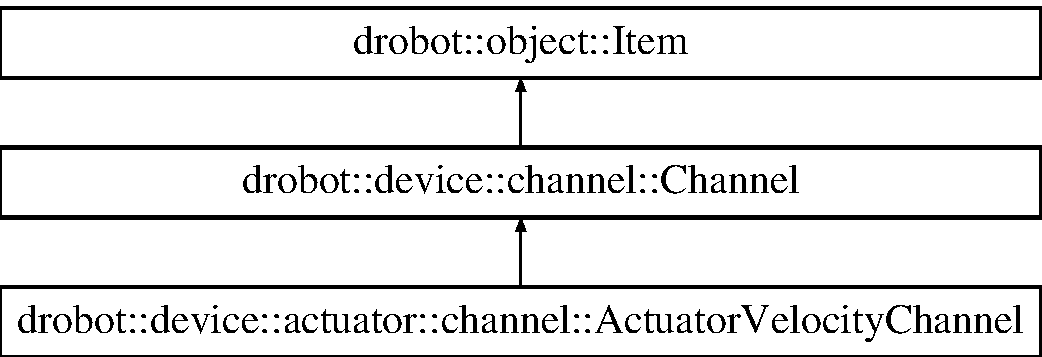
\includegraphics[height=3.000000cm]{classdrobot_1_1device_1_1actuator_1_1channel_1_1ActuatorVelocityChannel}
\end{center}
\end{figure}
\subsection*{Public Member Functions}
\begin{DoxyCompactItemize}
\item 
\hypertarget{classdrobot_1_1device_1_1actuator_1_1channel_1_1ActuatorVelocityChannel_ada31c8c19a9238563476adc37e2c515d}{{\bfseries Actuator\-Velocity\-Channel} (std\-::string name, device\-::channel\-::\-Channel\-Type type)}\label{classdrobot_1_1device_1_1actuator_1_1channel_1_1ActuatorVelocityChannel_ada31c8c19a9238563476adc37e2c515d}

\item 
\hypertarget{classdrobot_1_1device_1_1actuator_1_1channel_1_1ActuatorVelocityChannel_a961996b980471228a30b19136b8f43e1}{{\bfseries Actuator\-Velocity\-Channel} (std\-::string name, device\-::channel\-::\-Channel\-Type type, \hyperlink{classdrobot_1_1device_1_1channel_1_1Normalizer}{device\-::channel\-::\-Normalizer} $\ast$normalizer, \hyperlink{classdrobot_1_1device_1_1Device}{device\-::\-Device} $\ast$device)}\label{classdrobot_1_1device_1_1actuator_1_1channel_1_1ActuatorVelocityChannel_a961996b980471228a30b19136b8f43e1}

\end{DoxyCompactItemize}
\subsection*{Protected Member Functions}
\begin{DoxyCompactItemize}
\item 
virtual void \hyperlink{classdrobot_1_1device_1_1actuator_1_1channel_1_1ActuatorVelocityChannel_aaf05bcc79a0db85e05f0ddd999b18ff8}{set\-Value} (double value)
\begin{DoxyCompactList}\small\item\em sets the value directly to the device \end{DoxyCompactList}\item 
virtual double \hyperlink{classdrobot_1_1device_1_1actuator_1_1channel_1_1ActuatorVelocityChannel_a2d53e9dd788d9e9460ac5f8fa9ec513b}{get\-Value} ()
\begin{DoxyCompactList}\small\item\em returns the value directly from the device. \end{DoxyCompactList}\end{DoxyCompactItemize}
\subsection*{Additional Inherited Members}


\subsection{Member Function Documentation}
\hypertarget{classdrobot_1_1device_1_1actuator_1_1channel_1_1ActuatorVelocityChannel_a2d53e9dd788d9e9460ac5f8fa9ec513b}{\index{drobot\-::device\-::actuator\-::channel\-::\-Actuator\-Velocity\-Channel@{drobot\-::device\-::actuator\-::channel\-::\-Actuator\-Velocity\-Channel}!get\-Value@{get\-Value}}
\index{get\-Value@{get\-Value}!drobot::device::actuator::channel::ActuatorVelocityChannel@{drobot\-::device\-::actuator\-::channel\-::\-Actuator\-Velocity\-Channel}}
\subsubsection[{get\-Value}]{\setlength{\rightskip}{0pt plus 5cm}double drobot\-::device\-::actuator\-::channel\-::\-Actuator\-Velocity\-Channel\-::get\-Value (
\begin{DoxyParamCaption}
{}
\end{DoxyParamCaption}
)\hspace{0.3cm}{\ttfamily [protected]}, {\ttfamily [virtual]}}}\label{classdrobot_1_1device_1_1actuator_1_1channel_1_1ActuatorVelocityChannel_a2d53e9dd788d9e9460ac5f8fa9ec513b}


returns the value directly from the device. 

\begin{DoxyReturn}{Returns}

\end{DoxyReturn}


Implements \hyperlink{classdrobot_1_1device_1_1channel_1_1Channel_a42f0978ebb99d13a89c1785baf69a4d8}{drobot\-::device\-::channel\-::\-Channel}.

\hypertarget{classdrobot_1_1device_1_1actuator_1_1channel_1_1ActuatorVelocityChannel_aaf05bcc79a0db85e05f0ddd999b18ff8}{\index{drobot\-::device\-::actuator\-::channel\-::\-Actuator\-Velocity\-Channel@{drobot\-::device\-::actuator\-::channel\-::\-Actuator\-Velocity\-Channel}!set\-Value@{set\-Value}}
\index{set\-Value@{set\-Value}!drobot::device::actuator::channel::ActuatorVelocityChannel@{drobot\-::device\-::actuator\-::channel\-::\-Actuator\-Velocity\-Channel}}
\subsubsection[{set\-Value}]{\setlength{\rightskip}{0pt plus 5cm}void drobot\-::device\-::actuator\-::channel\-::\-Actuator\-Velocity\-Channel\-::set\-Value (
\begin{DoxyParamCaption}
\item[{double}]{value}
\end{DoxyParamCaption}
)\hspace{0.3cm}{\ttfamily [protected]}, {\ttfamily [virtual]}}}\label{classdrobot_1_1device_1_1actuator_1_1channel_1_1ActuatorVelocityChannel_aaf05bcc79a0db85e05f0ddd999b18ff8}


sets the value directly to the device 


\begin{DoxyParams}{Parameters}
{\em value} & \\
\hline
\end{DoxyParams}


Implements \hyperlink{classdrobot_1_1device_1_1channel_1_1Channel_a612a3f6afe59e238583d6d40d9ddcaf8}{drobot\-::device\-::channel\-::\-Channel}.



The documentation for this class was generated from the following files\-:\begin{DoxyCompactItemize}
\item 
src/drobot/device/actuator/channel/actuatorvelocitychannel.\-h\item 
src/drobot/device/actuator/channel/actuatorvelocitychannel.\-cpp\end{DoxyCompactItemize}

\hypertarget{classdrobot_1_1device_1_1actuator_1_1channel_1_1ActuatorVelocityChannelFactory}{\section{drobot\-:\-:device\-:\-:actuator\-:\-:channel\-:\-:Actuator\-Velocity\-Channel\-Factory Class Reference}
\label{classdrobot_1_1device_1_1actuator_1_1channel_1_1ActuatorVelocityChannelFactory}\index{drobot\-::device\-::actuator\-::channel\-::\-Actuator\-Velocity\-Channel\-Factory@{drobot\-::device\-::actuator\-::channel\-::\-Actuator\-Velocity\-Channel\-Factory}}
}
Inheritance diagram for drobot\-:\-:device\-:\-:actuator\-:\-:channel\-:\-:Actuator\-Velocity\-Channel\-Factory\-:\begin{figure}[H]
\begin{center}
\leavevmode
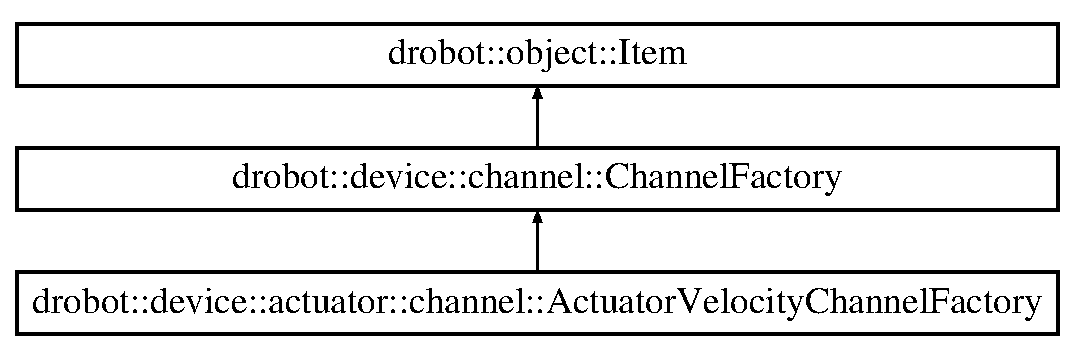
\includegraphics[height=3.000000cm]{classdrobot_1_1device_1_1actuator_1_1channel_1_1ActuatorVelocityChannelFactory}
\end{center}
\end{figure}
\subsection*{Public Member Functions}
\begin{DoxyCompactItemize}
\item 
virtual void \hyperlink{classdrobot_1_1device_1_1actuator_1_1channel_1_1ActuatorVelocityChannelFactory_ae60b06b9376c9b142137d97849dc8659}{create\-From\-Dom\-Element} (Q\-Dom\-Element element, \hyperlink{classdrobot_1_1device_1_1Device}{Device} $\ast$device)
\begin{DoxyCompactList}\small\item\em create channel from Dom Tree element \end{DoxyCompactList}\end{DoxyCompactItemize}
\subsection*{Additional Inherited Members}


\subsection{Member Function Documentation}
\hypertarget{classdrobot_1_1device_1_1actuator_1_1channel_1_1ActuatorVelocityChannelFactory_ae60b06b9376c9b142137d97849dc8659}{\index{drobot\-::device\-::actuator\-::channel\-::\-Actuator\-Velocity\-Channel\-Factory@{drobot\-::device\-::actuator\-::channel\-::\-Actuator\-Velocity\-Channel\-Factory}!create\-From\-Dom\-Element@{create\-From\-Dom\-Element}}
\index{create\-From\-Dom\-Element@{create\-From\-Dom\-Element}!drobot::device::actuator::channel::ActuatorVelocityChannelFactory@{drobot\-::device\-::actuator\-::channel\-::\-Actuator\-Velocity\-Channel\-Factory}}
\subsubsection[{create\-From\-Dom\-Element}]{\setlength{\rightskip}{0pt plus 5cm}void drobot\-::device\-::actuator\-::channel\-::\-Actuator\-Velocity\-Channel\-Factory\-::create\-From\-Dom\-Element (
\begin{DoxyParamCaption}
\item[{Q\-Dom\-Element}]{element, }
\item[{{\bf Device} $\ast$}]{device}
\end{DoxyParamCaption}
)\hspace{0.3cm}{\ttfamily [virtual]}}}\label{classdrobot_1_1device_1_1actuator_1_1channel_1_1ActuatorVelocityChannelFactory_ae60b06b9376c9b142137d97849dc8659}


create channel from Dom Tree element 

this method has to create one or more channels from the element and add it to the device. 
\begin{DoxyParams}{Parameters}
{\em element} & \\
\hline
{\em device} & \\
\hline
\end{DoxyParams}


Implements \hyperlink{classdrobot_1_1device_1_1channel_1_1ChannelFactory_ab59ee44782347b8878a471bf87f06c43}{drobot\-::device\-::channel\-::\-Channel\-Factory}.



The documentation for this class was generated from the following files\-:\begin{DoxyCompactItemize}
\item 
/home/imanol/workspace/drobot/new/src/drobot/device/actuator/channel/actuatorvelocitychannelfactory.\-h\item 
/home/imanol/workspace/drobot/new/src/drobot/device/actuator/channel/actuatorvelocitychannelfactory.\-cpp\end{DoxyCompactItemize}

\hypertarget{classdrobot_1_1device_1_1channel_1_1Channel}{\section{drobot\-:\-:device\-:\-:channel\-:\-:Channel Class Reference}
\label{classdrobot_1_1device_1_1channel_1_1Channel}\index{drobot\-::device\-::channel\-::\-Channel@{drobot\-::device\-::channel\-::\-Channel}}
}


The \hyperlink{classdrobot_1_1device_1_1channel_1_1Channel}{Channel} class is used to handle inputs and outputs from devices and log values.  




{\ttfamily \#include $<$channel.\-h$>$}

Inheritance diagram for drobot\-:\-:device\-:\-:channel\-:\-:Channel\-:\begin{figure}[H]
\begin{center}
\leavevmode
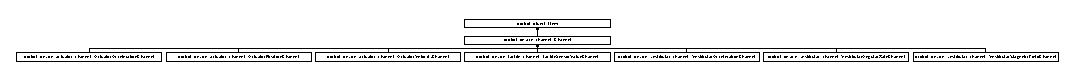
\includegraphics[height=0.597015cm]{classdrobot_1_1device_1_1channel_1_1Channel}
\end{center}
\end{figure}
\subsection*{Public Member Functions}
\begin{DoxyCompactItemize}
\item 
\hypertarget{classdrobot_1_1device_1_1channel_1_1Channel_a6fdb874d6679679e8b13cbcb94ab262c}{{\bfseries Channel} (std\-::string name, Channel\-Type type)}\label{classdrobot_1_1device_1_1channel_1_1Channel_a6fdb874d6679679e8b13cbcb94ab262c}

\item 
\hypertarget{classdrobot_1_1device_1_1channel_1_1Channel_ae86d5f4f5b0ad0438f1394fd433e6654}{{\bfseries Channel} (std\-::string name, Channel\-Type type, \hyperlink{classdrobot_1_1device_1_1channel_1_1Normalizer}{Normalizer} $\ast$normalizer, \hyperlink{classdrobot_1_1device_1_1Device}{Device} $\ast$device)}\label{classdrobot_1_1device_1_1channel_1_1Channel_ae86d5f4f5b0ad0438f1394fd433e6654}

\item 
\hypertarget{classdrobot_1_1device_1_1channel_1_1Channel_a86d35d028e0168f8058273ea28d71674}{void {\bfseries set\-Normalizer} (\hyperlink{classdrobot_1_1device_1_1channel_1_1Normalizer}{Normalizer} $\ast$normalizer)}\label{classdrobot_1_1device_1_1channel_1_1Channel_a86d35d028e0168f8058273ea28d71674}

\item 
\hypertarget{classdrobot_1_1device_1_1channel_1_1Channel_a2112fb19fbc17cc0b92188b84475c751}{\hyperlink{classdrobot_1_1device_1_1channel_1_1Normalizer}{Normalizer} $\ast$ {\bfseries get\-Normalizer} ()}\label{classdrobot_1_1device_1_1channel_1_1Channel_a2112fb19fbc17cc0b92188b84475c751}

\item 
\hypertarget{classdrobot_1_1device_1_1channel_1_1Channel_aae85170a5e749e6df36386a314132493}{void {\bfseries set\-Device} (\hyperlink{classdrobot_1_1device_1_1Device}{Device} $\ast$device)}\label{classdrobot_1_1device_1_1channel_1_1Channel_aae85170a5e749e6df36386a314132493}

\item 
\hypertarget{classdrobot_1_1device_1_1channel_1_1Channel_adc698d8fcdb9d571568f3958f865f514}{\hyperlink{classdrobot_1_1device_1_1Device}{Device} $\ast$ {\bfseries get\-Device} ()}\label{classdrobot_1_1device_1_1channel_1_1Channel_adc698d8fcdb9d571568f3958f865f514}

\item 
void \hyperlink{classdrobot_1_1device_1_1channel_1_1Channel_a2e70ae236c4c8d84f496fae813b387df}{set\-Normalized\-Value} (double value)
\begin{DoxyCompactList}\small\item\em set value in a normalized scale \end{DoxyCompactList}\item 
double \hyperlink{classdrobot_1_1device_1_1channel_1_1Channel_a15332594079b2c71afe11c9dd3cc93ab}{get\-Normalized\-Value} ()
\begin{DoxyCompactList}\small\item\em get\-Normalized\-Value \end{DoxyCompactList}\item 
void \hyperlink{classdrobot_1_1device_1_1channel_1_1Channel_a0ed4b6ec85cf797be7d60bdd8dc4a727}{set\-Real\-Value} (double value)
\begin{DoxyCompactList}\small\item\em sets the value in the device recognizable format \end{DoxyCompactList}\item 
double \hyperlink{classdrobot_1_1device_1_1channel_1_1Channel_ac292e30111718032a812cc682ac75657}{get\-Real\-Value} ()
\begin{DoxyCompactList}\small\item\em get\-Real\-Value \end{DoxyCompactList}\item 
\hypertarget{classdrobot_1_1device_1_1channel_1_1Channel_a353f70634d7475c92625400912278978}{std\-::string {\bfseries get\-Name} ()}\label{classdrobot_1_1device_1_1channel_1_1Channel_a353f70634d7475c92625400912278978}

\item 
\hypertarget{classdrobot_1_1device_1_1channel_1_1Channel_ad8ad9f811ec340ac58df6f92ed7400a1}{void {\bfseries set\-Type} (Channel\-Type type)}\label{classdrobot_1_1device_1_1channel_1_1Channel_ad8ad9f811ec340ac58df6f92ed7400a1}

\item 
\hypertarget{classdrobot_1_1device_1_1channel_1_1Channel_aa7f53c1709e13a86c1aac1562e2d7f2a}{Channel\-Type {\bfseries get\-Type} ()}\label{classdrobot_1_1device_1_1channel_1_1Channel_aa7f53c1709e13a86c1aac1562e2d7f2a}

\item 
void \hyperlink{classdrobot_1_1device_1_1channel_1_1Channel_a47ef77f7b66378313f1bcf9111a770f7}{read} ()
\begin{DoxyCompactList}\small\item\em read value from device \end{DoxyCompactList}\item 
void \hyperlink{classdrobot_1_1device_1_1channel_1_1Channel_ab938866883805ed5e68377f3e964b62e}{write} ()
\begin{DoxyCompactList}\small\item\em write value to device \end{DoxyCompactList}\end{DoxyCompactItemize}
\subsection*{Protected Member Functions}
\begin{DoxyCompactItemize}
\item 
virtual double \hyperlink{classdrobot_1_1device_1_1channel_1_1Channel_a42f0978ebb99d13a89c1785baf69a4d8}{get\-Value} ()=0
\begin{DoxyCompactList}\small\item\em returns the value directly from the device. \end{DoxyCompactList}\item 
virtual void \hyperlink{classdrobot_1_1device_1_1channel_1_1Channel_a612a3f6afe59e238583d6d40d9ddcaf8}{set\-Value} (double value)=0
\begin{DoxyCompactList}\small\item\em sets the value directly to the device \end{DoxyCompactList}\end{DoxyCompactItemize}
\subsection*{Protected Attributes}
\begin{DoxyCompactItemize}
\item 
\hypertarget{classdrobot_1_1device_1_1channel_1_1Channel_a065b4c1728f3756ac171c5191b780ff3}{\hyperlink{classdrobot_1_1device_1_1Device}{Device} $\ast$ \hyperlink{classdrobot_1_1device_1_1channel_1_1Channel_a065b4c1728f3756ac171c5191b780ff3}{\-\_\-device}}\label{classdrobot_1_1device_1_1channel_1_1Channel_a065b4c1728f3756ac171c5191b780ff3}

\begin{DoxyCompactList}\small\item\em the device this \hyperlink{classdrobot_1_1device_1_1channel_1_1Channel}{Channel} belongs to \end{DoxyCompactList}\end{DoxyCompactItemize}
\subsection*{Private Attributes}
\begin{DoxyCompactItemize}
\item 
\hypertarget{classdrobot_1_1device_1_1channel_1_1Channel_a1f141dd820e286c226aa91069527b8f7}{\hyperlink{classdrobot_1_1device_1_1channel_1_1Normalizer}{Normalizer} $\ast$ \hyperlink{classdrobot_1_1device_1_1channel_1_1Channel_a1f141dd820e286c226aa91069527b8f7}{\-\_\-normalizer}}\label{classdrobot_1_1device_1_1channel_1_1Channel_a1f141dd820e286c226aa91069527b8f7}

\begin{DoxyCompactList}\small\item\em \-\_\-normalizer used to convert the real\-Value to a normalized value between 0 and 1 and back again. \end{DoxyCompactList}\item 
\hypertarget{classdrobot_1_1device_1_1channel_1_1Channel_a5833ff457f5a59ad06f6e201056c6f1d}{Channel\-Type \hyperlink{classdrobot_1_1device_1_1channel_1_1Channel_a5833ff457f5a59ad06f6e201056c6f1d}{\-\_\-type}}\label{classdrobot_1_1device_1_1channel_1_1Channel_a5833ff457f5a59ad06f6e201056c6f1d}

\begin{DoxyCompactList}\small\item\em \-\_\-type of the channel \end{DoxyCompactList}\item 
\hypertarget{classdrobot_1_1device_1_1channel_1_1Channel_a636ff496310f897ba9b877285152f859}{double \hyperlink{classdrobot_1_1device_1_1channel_1_1Channel_a636ff496310f897ba9b877285152f859}{\-\_\-value}}\label{classdrobot_1_1device_1_1channel_1_1Channel_a636ff496310f897ba9b877285152f859}

\begin{DoxyCompactList}\small\item\em \-\_\-value serves as a cache \end{DoxyCompactList}\item 
\hypertarget{classdrobot_1_1device_1_1channel_1_1Channel_ab34987fd04666bc36f0962b23de48faa}{bool \hyperlink{classdrobot_1_1device_1_1channel_1_1Channel_ab34987fd04666bc36f0962b23de48faa}{\-\_\-update}}\label{classdrobot_1_1device_1_1channel_1_1Channel_ab34987fd04666bc36f0962b23de48faa}

\begin{DoxyCompactList}\small\item\em \-\_\-update true if output has been set during this timestep. Tells the system to set the value to the device via set\-Device() \end{DoxyCompactList}\end{DoxyCompactItemize}


\subsection{Detailed Description}
The \hyperlink{classdrobot_1_1device_1_1channel_1_1Channel}{Channel} class is used to handle inputs and outputs from devices and log values. 

The \hyperlink{classdrobot_1_1device_1_1channel_1_1Channel}{Channel} represents a property of a physical or virtual (simulated) device or simply a value you want to log. During runtime on each time step first all the read methods of the robot's channels are executed. The \hyperlink{classdrobot_1_1device_1_1channel_1_1Channel_a47ef77f7b66378313f1bcf9111a770f7}{read()} method takes the current value via the \hyperlink{classdrobot_1_1device_1_1channel_1_1Channel_a42f0978ebb99d13a89c1785baf69a4d8}{get\-Value()} method and copies it into the \-\_\-value property (if it is an input). Then the controller takes the inputs and calculates the outputs. These are set via \hyperlink{classdrobot_1_1device_1_1channel_1_1Channel_a0ed4b6ec85cf797be7d60bdd8dc4a727}{set\-Real\-Value()} or \hyperlink{classdrobot_1_1device_1_1channel_1_1Channel_a2e70ae236c4c8d84f496fae813b387df}{set\-Normalized\-Value()} to the \-\_\-value property. After the \hyperlink{classdrobot_1_1device_1_1channel_1_1Channel_ab938866883805ed5e68377f3e964b62e}{write()} method is executed which set's the \-\_\-value to the device via the \hyperlink{classdrobot_1_1device_1_1channel_1_1Channel_a612a3f6afe59e238583d6d40d9ddcaf8}{set\-Value()} method. For details see the \hyperlink{classdrobot_1_1robot_1_1Robot}{robot\-::\-Robot} and \hyperlink{classdrobot_1_1robot_1_1Controller}{robot\-::\-Controller} classes. 

\subsection{Member Function Documentation}
\hypertarget{classdrobot_1_1device_1_1channel_1_1Channel_a15332594079b2c71afe11c9dd3cc93ab}{\index{drobot\-::device\-::channel\-::\-Channel@{drobot\-::device\-::channel\-::\-Channel}!get\-Normalized\-Value@{get\-Normalized\-Value}}
\index{get\-Normalized\-Value@{get\-Normalized\-Value}!drobot::device::channel::Channel@{drobot\-::device\-::channel\-::\-Channel}}
\subsubsection[{get\-Normalized\-Value}]{\setlength{\rightskip}{0pt plus 5cm}double drobot\-::device\-::channel\-::\-Channel\-::get\-Normalized\-Value (
\begin{DoxyParamCaption}
{}
\end{DoxyParamCaption}
)}}\label{classdrobot_1_1device_1_1channel_1_1Channel_a15332594079b2c71afe11c9dd3cc93ab}


get\-Normalized\-Value 

\begin{DoxyReturn}{Returns}
the normalized value 
\end{DoxyReturn}
\hypertarget{classdrobot_1_1device_1_1channel_1_1Channel_ac292e30111718032a812cc682ac75657}{\index{drobot\-::device\-::channel\-::\-Channel@{drobot\-::device\-::channel\-::\-Channel}!get\-Real\-Value@{get\-Real\-Value}}
\index{get\-Real\-Value@{get\-Real\-Value}!drobot::device::channel::Channel@{drobot\-::device\-::channel\-::\-Channel}}
\subsubsection[{get\-Real\-Value}]{\setlength{\rightskip}{0pt plus 5cm}double drobot\-::device\-::channel\-::\-Channel\-::get\-Real\-Value (
\begin{DoxyParamCaption}
{}
\end{DoxyParamCaption}
)}}\label{classdrobot_1_1device_1_1channel_1_1Channel_ac292e30111718032a812cc682ac75657}


get\-Real\-Value 

\begin{DoxyReturn}{Returns}
the real value 
\end{DoxyReturn}
\hypertarget{classdrobot_1_1device_1_1channel_1_1Channel_a42f0978ebb99d13a89c1785baf69a4d8}{\index{drobot\-::device\-::channel\-::\-Channel@{drobot\-::device\-::channel\-::\-Channel}!get\-Value@{get\-Value}}
\index{get\-Value@{get\-Value}!drobot::device::channel::Channel@{drobot\-::device\-::channel\-::\-Channel}}
\subsubsection[{get\-Value}]{\setlength{\rightskip}{0pt plus 5cm}virtual double drobot\-::device\-::channel\-::\-Channel\-::get\-Value (
\begin{DoxyParamCaption}
{}
\end{DoxyParamCaption}
)\hspace{0.3cm}{\ttfamily [protected]}, {\ttfamily [pure virtual]}}}\label{classdrobot_1_1device_1_1channel_1_1Channel_a42f0978ebb99d13a89c1785baf69a4d8}


returns the value directly from the device. 

\begin{DoxyReturn}{Returns}

\end{DoxyReturn}


Implemented in \hyperlink{classdrobot_1_1device_1_1vestibular_1_1channel_1_1VestibularAccelerationChannel_a5796705561dd541462ced1f514b17a04}{drobot\-::device\-::vestibular\-::channel\-::\-Vestibular\-Acceleration\-Channel}, \hyperlink{classdrobot_1_1device_1_1vestibular_1_1channel_1_1VestibularAngularRateChannel_a0a818f81ba8225d5444aad283faae683}{drobot\-::device\-::vestibular\-::channel\-::\-Vestibular\-Angular\-Rate\-Channel}, \hyperlink{classdrobot_1_1device_1_1vestibular_1_1channel_1_1VestibularMagneticFieldChannel_a3c5d0cb2b7c69dfcd11bc16e8a3a6c68}{drobot\-::device\-::vestibular\-::channel\-::\-Vestibular\-Magnetic\-Field\-Channel}, \hyperlink{classdrobot_1_1device_1_1actuator_1_1channel_1_1ActuatorAccelerationChannel_a8dab242bd8099a88a2fd981508827224}{drobot\-::device\-::actuator\-::channel\-::\-Actuator\-Acceleration\-Channel}, \hyperlink{classdrobot_1_1device_1_1actuator_1_1channel_1_1ActuatorPositionChannel_a21dd5208fd7d5c439d711871cfbbea9a}{drobot\-::device\-::actuator\-::channel\-::\-Actuator\-Position\-Channel}, \hyperlink{classdrobot_1_1device_1_1actuator_1_1channel_1_1ActuatorVelocityChannel_a2d53e9dd788d9e9460ac5f8fa9ec513b}{drobot\-::device\-::actuator\-::channel\-::\-Actuator\-Velocity\-Channel}, and \hyperlink{classdrobot_1_1device_1_1tactile_1_1channel_1_1TactileSensorValueChannel_a84465511da1c70beb14508828243ff6d}{drobot\-::device\-::tactile\-::channel\-::\-Tactile\-Sensor\-Value\-Channel}.

\hypertarget{classdrobot_1_1device_1_1channel_1_1Channel_a47ef77f7b66378313f1bcf9111a770f7}{\index{drobot\-::device\-::channel\-::\-Channel@{drobot\-::device\-::channel\-::\-Channel}!read@{read}}
\index{read@{read}!drobot::device::channel::Channel@{drobot\-::device\-::channel\-::\-Channel}}
\subsubsection[{read}]{\setlength{\rightskip}{0pt plus 5cm}void drobot\-::device\-::channel\-::\-Channel\-::read (
\begin{DoxyParamCaption}
{}
\end{DoxyParamCaption}
)}}\label{classdrobot_1_1device_1_1channel_1_1Channel_a47ef77f7b66378313f1bcf9111a770f7}


read value from device 

copies the value from the device to the \-\_\-value property using \hyperlink{classdrobot_1_1device_1_1channel_1_1Channel_a42f0978ebb99d13a89c1785baf69a4d8}{get\-Value()} if it is an input channel. \hypertarget{classdrobot_1_1device_1_1channel_1_1Channel_a2e70ae236c4c8d84f496fae813b387df}{\index{drobot\-::device\-::channel\-::\-Channel@{drobot\-::device\-::channel\-::\-Channel}!set\-Normalized\-Value@{set\-Normalized\-Value}}
\index{set\-Normalized\-Value@{set\-Normalized\-Value}!drobot::device::channel::Channel@{drobot\-::device\-::channel\-::\-Channel}}
\subsubsection[{set\-Normalized\-Value}]{\setlength{\rightskip}{0pt plus 5cm}void drobot\-::device\-::channel\-::\-Channel\-::set\-Normalized\-Value (
\begin{DoxyParamCaption}
\item[{double}]{value}
\end{DoxyParamCaption}
)}}\label{classdrobot_1_1device_1_1channel_1_1Channel_a2e70ae236c4c8d84f496fae813b387df}


set value in a normalized scale 

set a normalized value to this channel (for instance an output from a neural network). Is automatically converted to a device recognizable value. 
\begin{DoxyParams}{Parameters}
{\em value} & \\
\hline
\end{DoxyParams}
\hypertarget{classdrobot_1_1device_1_1channel_1_1Channel_a0ed4b6ec85cf797be7d60bdd8dc4a727}{\index{drobot\-::device\-::channel\-::\-Channel@{drobot\-::device\-::channel\-::\-Channel}!set\-Real\-Value@{set\-Real\-Value}}
\index{set\-Real\-Value@{set\-Real\-Value}!drobot::device::channel::Channel@{drobot\-::device\-::channel\-::\-Channel}}
\subsubsection[{set\-Real\-Value}]{\setlength{\rightskip}{0pt plus 5cm}void drobot\-::device\-::channel\-::\-Channel\-::set\-Real\-Value (
\begin{DoxyParamCaption}
\item[{double}]{value}
\end{DoxyParamCaption}
)}}\label{classdrobot_1_1device_1_1channel_1_1Channel_a0ed4b6ec85cf797be7d60bdd8dc4a727}


sets the value in the device recognizable format 


\begin{DoxyParams}{Parameters}
{\em value} & \\
\hline
\end{DoxyParams}
\hypertarget{classdrobot_1_1device_1_1channel_1_1Channel_a612a3f6afe59e238583d6d40d9ddcaf8}{\index{drobot\-::device\-::channel\-::\-Channel@{drobot\-::device\-::channel\-::\-Channel}!set\-Value@{set\-Value}}
\index{set\-Value@{set\-Value}!drobot::device::channel::Channel@{drobot\-::device\-::channel\-::\-Channel}}
\subsubsection[{set\-Value}]{\setlength{\rightskip}{0pt plus 5cm}virtual void drobot\-::device\-::channel\-::\-Channel\-::set\-Value (
\begin{DoxyParamCaption}
\item[{double}]{value}
\end{DoxyParamCaption}
)\hspace{0.3cm}{\ttfamily [protected]}, {\ttfamily [pure virtual]}}}\label{classdrobot_1_1device_1_1channel_1_1Channel_a612a3f6afe59e238583d6d40d9ddcaf8}


sets the value directly to the device 


\begin{DoxyParams}{Parameters}
{\em value} & \\
\hline
\end{DoxyParams}


Implemented in \hyperlink{classdrobot_1_1device_1_1vestibular_1_1channel_1_1VestibularAccelerationChannel_a27c4b430ad0280cc34cfe1b888d2211a}{drobot\-::device\-::vestibular\-::channel\-::\-Vestibular\-Acceleration\-Channel}, \hyperlink{classdrobot_1_1device_1_1vestibular_1_1channel_1_1VestibularAngularRateChannel_a6ad7884779e51539bbbc81f1b8e8799b}{drobot\-::device\-::vestibular\-::channel\-::\-Vestibular\-Angular\-Rate\-Channel}, \hyperlink{classdrobot_1_1device_1_1vestibular_1_1channel_1_1VestibularMagneticFieldChannel_add412ebf9daf0eb491eae4ce14772a8c}{drobot\-::device\-::vestibular\-::channel\-::\-Vestibular\-Magnetic\-Field\-Channel}, \hyperlink{classdrobot_1_1device_1_1actuator_1_1channel_1_1ActuatorAccelerationChannel_a33cdc24b62518961f8c003a31097c48d}{drobot\-::device\-::actuator\-::channel\-::\-Actuator\-Acceleration\-Channel}, \hyperlink{classdrobot_1_1device_1_1actuator_1_1channel_1_1ActuatorPositionChannel_ac293318a0e51a0cca153326efd08d7c8}{drobot\-::device\-::actuator\-::channel\-::\-Actuator\-Position\-Channel}, \hyperlink{classdrobot_1_1device_1_1actuator_1_1channel_1_1ActuatorVelocityChannel_aaf05bcc79a0db85e05f0ddd999b18ff8}{drobot\-::device\-::actuator\-::channel\-::\-Actuator\-Velocity\-Channel}, and \hyperlink{classdrobot_1_1device_1_1tactile_1_1channel_1_1TactileSensorValueChannel_af98159e60d1bc3ebfff9135c179f4287}{drobot\-::device\-::tactile\-::channel\-::\-Tactile\-Sensor\-Value\-Channel}.

\hypertarget{classdrobot_1_1device_1_1channel_1_1Channel_ab938866883805ed5e68377f3e964b62e}{\index{drobot\-::device\-::channel\-::\-Channel@{drobot\-::device\-::channel\-::\-Channel}!write@{write}}
\index{write@{write}!drobot::device::channel::Channel@{drobot\-::device\-::channel\-::\-Channel}}
\subsubsection[{write}]{\setlength{\rightskip}{0pt plus 5cm}void drobot\-::device\-::channel\-::\-Channel\-::write (
\begin{DoxyParamCaption}
{}
\end{DoxyParamCaption}
)}}\label{classdrobot_1_1device_1_1channel_1_1Channel_ab938866883805ed5e68377f3e964b62e}


write value to device 

writes the value from the \-\_\-value property to the device using \hyperlink{classdrobot_1_1device_1_1channel_1_1Channel_a612a3f6afe59e238583d6d40d9ddcaf8}{set\-Value()} if it is an output channel and a value has been set since the last call of \hyperlink{classdrobot_1_1device_1_1channel_1_1Channel_ab938866883805ed5e68377f3e964b62e}{write()}. 

The documentation for this class was generated from the following files\-:\begin{DoxyCompactItemize}
\item 
/home/imanol/workspace/drobot/new/src/drobot/device/channel/channel.\-h\item 
/home/imanol/workspace/drobot/new/src/drobot/device/channel/channel.\-cpp\end{DoxyCompactItemize}

\hypertarget{classdrobot_1_1device_1_1channel_1_1ChannelFactory}{\section{drobot\-:\-:device\-:\-:channel\-:\-:Channel\-Factory Class Reference}
\label{classdrobot_1_1device_1_1channel_1_1ChannelFactory}\index{drobot\-::device\-::channel\-::\-Channel\-Factory@{drobot\-::device\-::channel\-::\-Channel\-Factory}}
}


The \hyperlink{classdrobot_1_1device_1_1channel_1_1ChannelFactory}{Channel\-Factory} class.  




{\ttfamily \#include $<$channelfactory.\-h$>$}

Inheritance diagram for drobot\-:\-:device\-:\-:channel\-:\-:Channel\-Factory\-:\begin{figure}[H]
\begin{center}
\leavevmode
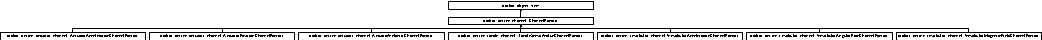
\includegraphics[height=0.538117cm]{classdrobot_1_1device_1_1channel_1_1ChannelFactory}
\end{center}
\end{figure}
\subsection*{Public Member Functions}
\begin{DoxyCompactItemize}
\item 
\hypertarget{classdrobot_1_1device_1_1channel_1_1ChannelFactory_ab563684681065c52b85620d60b2abdf8}{{\bfseries Channel\-Factory} (std\-::string name)}\label{classdrobot_1_1device_1_1channel_1_1ChannelFactory_ab563684681065c52b85620d60b2abdf8}

\item 
virtual void \hyperlink{classdrobot_1_1device_1_1channel_1_1ChannelFactory_ab59ee44782347b8878a471bf87f06c43}{create\-From\-Dom\-Element} (Q\-Dom\-Element element, \hyperlink{classdrobot_1_1device_1_1Device}{Device} $\ast$device)=0
\begin{DoxyCompactList}\small\item\em create channel from Dom Tree element \end{DoxyCompactList}\end{DoxyCompactItemize}
\subsection*{Additional Inherited Members}


\subsection{Detailed Description}
The \hyperlink{classdrobot_1_1device_1_1channel_1_1ChannelFactory}{Channel\-Factory} class. 

used to create a channel from a Dom Tree element (Q\-Dom\-Element) and add it to a device. The name of the \hyperlink{classdrobot_1_1device_1_1channel_1_1ChannelFactory}{Channel\-Factory} must be the same as the tag\-Name of the xml elements. 

\subsection{Member Function Documentation}
\hypertarget{classdrobot_1_1device_1_1channel_1_1ChannelFactory_ab59ee44782347b8878a471bf87f06c43}{\index{drobot\-::device\-::channel\-::\-Channel\-Factory@{drobot\-::device\-::channel\-::\-Channel\-Factory}!create\-From\-Dom\-Element@{create\-From\-Dom\-Element}}
\index{create\-From\-Dom\-Element@{create\-From\-Dom\-Element}!drobot::device::channel::ChannelFactory@{drobot\-::device\-::channel\-::\-Channel\-Factory}}
\subsubsection[{create\-From\-Dom\-Element}]{\setlength{\rightskip}{0pt plus 5cm}virtual void drobot\-::device\-::channel\-::\-Channel\-Factory\-::create\-From\-Dom\-Element (
\begin{DoxyParamCaption}
\item[{Q\-Dom\-Element}]{element, }
\item[{{\bf Device} $\ast$}]{device}
\end{DoxyParamCaption}
)\hspace{0.3cm}{\ttfamily [pure virtual]}}}\label{classdrobot_1_1device_1_1channel_1_1ChannelFactory_ab59ee44782347b8878a471bf87f06c43}


create channel from Dom Tree element 

this method has to create one or more channels from the element and add it to the device. 
\begin{DoxyParams}{Parameters}
{\em element} & \\
\hline
{\em device} & \\
\hline
\end{DoxyParams}


Implemented in \hyperlink{classdrobot_1_1device_1_1actuator_1_1channel_1_1ActuatorAccelerationChannelFactory_a077744d3866b134b15cfe9522eeb99e3}{drobot\-::device\-::actuator\-::channel\-::\-Actuator\-Acceleration\-Channel\-Factory}, \hyperlink{classdrobot_1_1device_1_1actuator_1_1channel_1_1ActuatorPositionChannelFactory_a66d52953c14b0686b3dd61b9f8462476}{drobot\-::device\-::actuator\-::channel\-::\-Actuator\-Position\-Channel\-Factory}, \hyperlink{classdrobot_1_1device_1_1actuator_1_1channel_1_1ActuatorVelocityChannelFactory_ae60b06b9376c9b142137d97849dc8659}{drobot\-::device\-::actuator\-::channel\-::\-Actuator\-Velocity\-Channel\-Factory}, \hyperlink{classdrobot_1_1device_1_1vestibular_1_1channel_1_1VestibularAccelerationChannelFactory_a79214e8381183d99c9f27fc2abe41e59}{drobot\-::device\-::vestibular\-::channel\-::\-Vestibular\-Acceleration\-Channel\-Factory}, \hyperlink{classdrobot_1_1device_1_1vestibular_1_1channel_1_1VestibularAngularRateChannelFactory_a1a1dbc3b83511d7d50f7ff3e7bb12158}{drobot\-::device\-::vestibular\-::channel\-::\-Vestibular\-Angular\-Rate\-Channel\-Factory}, \hyperlink{classdrobot_1_1device_1_1vestibular_1_1channel_1_1VestibularMagneticFieldChannelFactory_a9eee36d4270b5beaa7e56a62bd916aa5}{drobot\-::device\-::vestibular\-::channel\-::\-Vestibular\-Magnetic\-Field\-Channel\-Factory}, and \hyperlink{classdrobot_1_1device_1_1tactile_1_1channel_1_1TactileSensorValueChannelFactory_a2e4369c57cdd99f2c59469f6451e4c0c}{drobot\-::device\-::tactile\-::channel\-::\-Tactile\-Sensor\-Value\-Channel\-Factory}.



The documentation for this class was generated from the following files\-:\begin{DoxyCompactItemize}
\item 
/home/imanol/workspace/drobot/new/src/drobot/device/channel/channelfactory.\-h\item 
/home/imanol/workspace/drobot/new/src/drobot/device/channel/channelfactory.\-cpp\end{DoxyCompactItemize}

\hypertarget{classdrobot_1_1device_1_1channel_1_1ChannelManager}{\section{drobot\-:\-:device\-:\-:channel\-:\-:Channel\-Manager Class Reference}
\label{classdrobot_1_1device_1_1channel_1_1ChannelManager}\index{drobot\-::device\-::channel\-::\-Channel\-Manager@{drobot\-::device\-::channel\-::\-Channel\-Manager}}
}


Special implementation of a Manager for \hyperlink{classdrobot_1_1device_1_1channel_1_1Channel}{Channel} Items.  




{\ttfamily \#include $<$channelmanager.\-h$>$}

Inheritance diagram for drobot\-:\-:device\-:\-:channel\-:\-:Channel\-Manager\-:\begin{figure}[H]
\begin{center}
\leavevmode
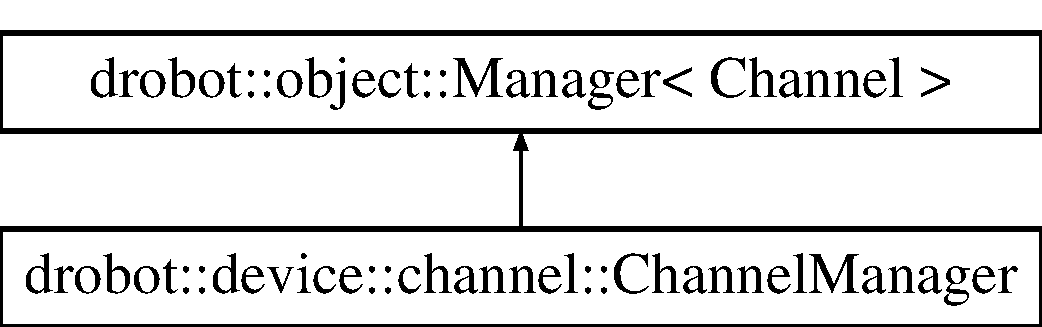
\includegraphics[height=2.000000cm]{classdrobot_1_1device_1_1channel_1_1ChannelManager}
\end{center}
\end{figure}
\subsection*{Public Member Functions}
\begin{DoxyCompactItemize}
\item 
\hypertarget{classdrobot_1_1device_1_1channel_1_1ChannelManager_aa5f87db0706bef4130d8e016f02178b2}{{\bfseries Channel\-Manager} (std\-::vector$<$ \hyperlink{classdrobot_1_1device_1_1channel_1_1Channel}{Channel} $\ast$ $>$ items)}\label{classdrobot_1_1device_1_1channel_1_1ChannelManager_aa5f87db0706bef4130d8e016f02178b2}

\item 
std\-::vector$<$ \hyperlink{classdrobot_1_1device_1_1channel_1_1Channel}{Channel} $\ast$ $>$ \hyperlink{classdrobot_1_1device_1_1channel_1_1ChannelManager_a24b3b63d09b4357a1632d8f8f0e7798b}{list\-By\-Type} (Channel\-Type type)
\begin{DoxyCompactList}\small\item\em returns channels filtered by type \end{DoxyCompactList}\item 
\hypertarget{classdrobot_1_1device_1_1channel_1_1ChannelManager_ad200adec504cad270c5da9d244bd2e28}{void \hyperlink{classdrobot_1_1device_1_1channel_1_1ChannelManager_ad200adec504cad270c5da9d244bd2e28}{read} ()}\label{classdrobot_1_1device_1_1channel_1_1ChannelManager_ad200adec504cad270c5da9d244bd2e28}

\begin{DoxyCompactList}\small\item\em executes the \hyperlink{classdrobot_1_1device_1_1channel_1_1ChannelManager_ad200adec504cad270c5da9d244bd2e28}{read()} method on all channels \end{DoxyCompactList}\item 
\hypertarget{classdrobot_1_1device_1_1channel_1_1ChannelManager_a103b360e79080b145bae8c81d33ba4c9}{void \hyperlink{classdrobot_1_1device_1_1channel_1_1ChannelManager_a103b360e79080b145bae8c81d33ba4c9}{write} ()}\label{classdrobot_1_1device_1_1channel_1_1ChannelManager_a103b360e79080b145bae8c81d33ba4c9}

\begin{DoxyCompactList}\small\item\em executes the \hyperlink{classdrobot_1_1device_1_1channel_1_1ChannelManager_a103b360e79080b145bae8c81d33ba4c9}{write()} method on all channels \end{DoxyCompactList}\end{DoxyCompactItemize}
\subsection*{Additional Inherited Members}


\subsection{Detailed Description}
Special implementation of a Manager for \hyperlink{classdrobot_1_1device_1_1channel_1_1Channel}{Channel} Items. 

\subsection{Member Function Documentation}
\hypertarget{classdrobot_1_1device_1_1channel_1_1ChannelManager_a24b3b63d09b4357a1632d8f8f0e7798b}{\index{drobot\-::device\-::channel\-::\-Channel\-Manager@{drobot\-::device\-::channel\-::\-Channel\-Manager}!list\-By\-Type@{list\-By\-Type}}
\index{list\-By\-Type@{list\-By\-Type}!drobot::device::channel::ChannelManager@{drobot\-::device\-::channel\-::\-Channel\-Manager}}
\subsubsection[{list\-By\-Type}]{\setlength{\rightskip}{0pt plus 5cm}std\-::vector$<$ {\bf Channel} $\ast$ $>$ drobot\-::device\-::channel\-::\-Channel\-Manager\-::list\-By\-Type (
\begin{DoxyParamCaption}
\item[{Channel\-Type}]{type}
\end{DoxyParamCaption}
)}}\label{classdrobot_1_1device_1_1channel_1_1ChannelManager_a24b3b63d09b4357a1632d8f8f0e7798b}


returns channels filtered by type 


\begin{DoxyParams}{Parameters}
{\em type} & \\
\hline
\end{DoxyParams}
\begin{DoxyReturn}{Returns}
channels 
\end{DoxyReturn}


The documentation for this class was generated from the following files\-:\begin{DoxyCompactItemize}
\item 
src/drobot/device/channel/channelmanager.\-h\item 
src/drobot/device/channel/channelmanager.\-cpp\end{DoxyCompactItemize}

\hypertarget{classdrobot_1_1util_1_1Clock}{\section{drobot\-:\-:util\-:\-:Clock Class Reference}
\label{classdrobot_1_1util_1_1Clock}\index{drobot\-::util\-::\-Clock@{drobot\-::util\-::\-Clock}}
}


The \hyperlink{classdrobot_1_1util_1_1Clock}{Clock} class can be used to synchronize a loop to a specific frequency.  




{\ttfamily \#include $<$clock.\-h$>$}

\subsection*{Public Member Functions}
\begin{DoxyCompactItemize}
\item 
\hypertarget{classdrobot_1_1util_1_1Clock_abbb34db76f1b1bdc73f4da74233df96e}{{\bfseries Clock} (double frequency)}\label{classdrobot_1_1util_1_1Clock_abbb34db76f1b1bdc73f4da74233df96e}

\item 
\hypertarget{classdrobot_1_1util_1_1Clock_a16c9d681c2d95e3cf3a8566e786eef4c}{void {\bfseries init} ()}\label{classdrobot_1_1util_1_1Clock_a16c9d681c2d95e3cf3a8566e786eef4c}

\item 
void \hyperlink{classdrobot_1_1util_1_1Clock_a7b9b7059c83a69a3805730e4101292ce}{wait\-For\-Tick} ()
\begin{DoxyCompactList}\small\item\em wait\-For\-Tick is used to wait for the next timestep. \end{DoxyCompactList}\item 
\hypertarget{classdrobot_1_1util_1_1Clock_a39c8b68b1d807ba60253e72b02a2ee23}{void {\bfseries set\-Frequency} (double frequency)}\label{classdrobot_1_1util_1_1Clock_a39c8b68b1d807ba60253e72b02a2ee23}

\item 
\hypertarget{classdrobot_1_1util_1_1Clock_af476d9c0904776c9457395b70385fab0}{double {\bfseries get\-Frequency} ()}\label{classdrobot_1_1util_1_1Clock_af476d9c0904776c9457395b70385fab0}

\end{DoxyCompactItemize}
\subsection*{Private Member Functions}
\begin{DoxyCompactItemize}
\item 
\hypertarget{classdrobot_1_1util_1_1Clock_a5fe7640381b84529990f33a221770000}{void {\bfseries unlock} ()}\label{classdrobot_1_1util_1_1Clock_a5fe7640381b84529990f33a221770000}

\end{DoxyCompactItemize}
\subsection*{Private Attributes}
\begin{DoxyCompactItemize}
\item 
\hypertarget{classdrobot_1_1util_1_1Clock_a01dd882e7407ed6a9f91b22a30ecfa81}{bool {\bfseries \-\_\-lock}}\label{classdrobot_1_1util_1_1Clock_a01dd882e7407ed6a9f91b22a30ecfa81}

\item 
\hypertarget{classdrobot_1_1util_1_1Clock_a947834caf07b8a062fde75969a299bb8}{double {\bfseries \-\_\-frequency}}\label{classdrobot_1_1util_1_1Clock_a947834caf07b8a062fde75969a299bb8}

\end{DoxyCompactItemize}


\subsection{Detailed Description}
The \hyperlink{classdrobot_1_1util_1_1Clock}{Clock} class can be used to synchronize a loop to a specific frequency. 

\subsection{Member Function Documentation}
\hypertarget{classdrobot_1_1util_1_1Clock_a7b9b7059c83a69a3805730e4101292ce}{\index{drobot\-::util\-::\-Clock@{drobot\-::util\-::\-Clock}!wait\-For\-Tick@{wait\-For\-Tick}}
\index{wait\-For\-Tick@{wait\-For\-Tick}!drobot::util::Clock@{drobot\-::util\-::\-Clock}}
\subsubsection[{wait\-For\-Tick}]{\setlength{\rightskip}{0pt plus 5cm}void drobot\-::util\-::\-Clock\-::wait\-For\-Tick (
\begin{DoxyParamCaption}
{}
\end{DoxyParamCaption}
)}}\label{classdrobot_1_1util_1_1Clock_a7b9b7059c83a69a3805730e4101292ce}


wait\-For\-Tick is used to wait for the next timestep. 

It returns immediately in the first call. After that it blocks until the next tick's time has arrived. This method should be called at the beginning of the loop. 

The documentation for this class was generated from the following files\-:\begin{DoxyCompactItemize}
\item 
src/drobot/util/clock.\-h\item 
src/drobot/util/clock.\-cpp\end{DoxyCompactItemize}

\hypertarget{classdrobot_1_1robot_1_1Controller}{\section{drobot\-:\-:robot\-:\-:Controller Class Reference}
\label{classdrobot_1_1robot_1_1Controller}\index{drobot\-::robot\-::\-Controller@{drobot\-::robot\-::\-Controller}}
}


Base class for \hyperlink{classdrobot_1_1robot_1_1Robot}{Robot} Controllers.  




{\ttfamily \#include $<$controller.\-h$>$}

Inheritance diagram for drobot\-:\-:robot\-:\-:Controller\-:\begin{figure}[H]
\begin{center}
\leavevmode
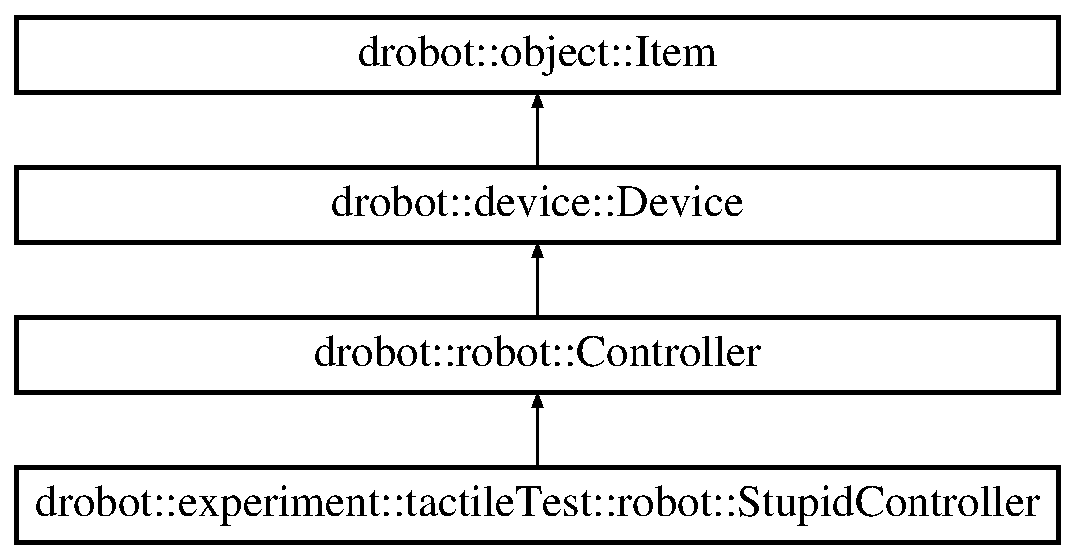
\includegraphics[height=4.000000cm]{classdrobot_1_1robot_1_1Controller}
\end{center}
\end{figure}
\subsection*{Public Member Functions}
\begin{DoxyCompactItemize}
\item 
\hypertarget{classdrobot_1_1robot_1_1Controller_af74be803a0338e75a68c59f444530948}{{\bfseries Controller} (std\-::string name)}\label{classdrobot_1_1robot_1_1Controller_af74be803a0338e75a68c59f444530948}

\item 
virtual void \hyperlink{classdrobot_1_1robot_1_1Controller_acbbde3e529dad162fb36074c7e25a924}{step} (long tick, \hyperlink{classdrobot_1_1device_1_1channel_1_1ChannelManager}{device\-::channel\-::\-Channel\-Manager} $\ast$channels)=0
\begin{DoxyCompactList}\small\item\em This function is called at a specific frequency defined in the \hyperlink{classdrobot_1_1robot_1_1Robot}{Robot}. \end{DoxyCompactList}\item 
\hypertarget{classdrobot_1_1robot_1_1Controller_afa7f38adf10288f9942e133cfdf26f3e}{void {\bfseries set\-Robot} (\hyperlink{classdrobot_1_1robot_1_1Robot}{Robot} $\ast$robot)}\label{classdrobot_1_1robot_1_1Controller_afa7f38adf10288f9942e133cfdf26f3e}

\item 
\hypertarget{classdrobot_1_1robot_1_1Controller_aaee713e766a87dec33c48308be4a5102}{\hyperlink{classdrobot_1_1robot_1_1Robot}{Robot} $\ast$ {\bfseries get\-Robot} ()}\label{classdrobot_1_1robot_1_1Controller_aaee713e766a87dec33c48308be4a5102}

\item 
virtual void \hyperlink{classdrobot_1_1robot_1_1Controller_a533a9761503d502c64c25538ce8eb35c}{enable} ()
\begin{DoxyCompactList}\small\item\em enables the device. \end{DoxyCompactList}\item 
virtual void \hyperlink{classdrobot_1_1robot_1_1Controller_a40384f970deab8157ada1ead78d8b383}{disable} ()
\begin{DoxyCompactList}\small\item\em disables the device. \end{DoxyCompactList}\item 
virtual bool \hyperlink{classdrobot_1_1robot_1_1Controller_a8f7c73ba2adb3f7c02ff97b5c9d94b12}{is\-Enabled} ()
\begin{DoxyCompactList}\small\item\em check if the device is enabled \end{DoxyCompactList}\end{DoxyCompactItemize}
\subsection*{Protected Attributes}
\begin{DoxyCompactItemize}
\item 
\hypertarget{classdrobot_1_1robot_1_1Controller_ae2ec0e60b65c7b56db0f5da9ee8c7b2d}{\hyperlink{classdrobot_1_1robot_1_1Robot}{Robot} $\ast$ \hyperlink{classdrobot_1_1robot_1_1Controller_ae2ec0e60b65c7b56db0f5da9ee8c7b2d}{\-\_\-robot}}\label{classdrobot_1_1robot_1_1Controller_ae2ec0e60b65c7b56db0f5da9ee8c7b2d}

\begin{DoxyCompactList}\small\item\em the robot being controlled \end{DoxyCompactList}\item 
\hypertarget{classdrobot_1_1robot_1_1Controller_a39de453e625818a2083c4393dba021f2}{bool {\bfseries \-\_\-enabled}}\label{classdrobot_1_1robot_1_1Controller_a39de453e625818a2083c4393dba021f2}

\end{DoxyCompactItemize}


\subsection{Detailed Description}
Base class for \hyperlink{classdrobot_1_1robot_1_1Robot}{Robot} Controllers. 

this class derives from the Device class so that you may add Channels of type L\-O\-G to it. See \hyperlink{classdrobot_1_1device_1_1channel_1_1Channel}{device\-::channel\-::\-Channel} for details. 

\subsection{Member Function Documentation}
\hypertarget{classdrobot_1_1robot_1_1Controller_a40384f970deab8157ada1ead78d8b383}{\index{drobot\-::robot\-::\-Controller@{drobot\-::robot\-::\-Controller}!disable@{disable}}
\index{disable@{disable}!drobot::robot::Controller@{drobot\-::robot\-::\-Controller}}
\subsubsection[{disable}]{\setlength{\rightskip}{0pt plus 5cm}void drobot\-::robot\-::\-Controller\-::disable (
\begin{DoxyParamCaption}
{}
\end{DoxyParamCaption}
)\hspace{0.3cm}{\ttfamily [virtual]}}}\label{classdrobot_1_1robot_1_1Controller_a40384f970deab8157ada1ead78d8b383}


disables the device. 

This function has to be implemented by the specific device. For physical devices like actuators this method should power off the device; 

Reimplemented from \hyperlink{classdrobot_1_1device_1_1Device_a289499673ae30bd72101c68fbd04cd89}{drobot\-::device\-::\-Device}.

\hypertarget{classdrobot_1_1robot_1_1Controller_a533a9761503d502c64c25538ce8eb35c}{\index{drobot\-::robot\-::\-Controller@{drobot\-::robot\-::\-Controller}!enable@{enable}}
\index{enable@{enable}!drobot::robot::Controller@{drobot\-::robot\-::\-Controller}}
\subsubsection[{enable}]{\setlength{\rightskip}{0pt plus 5cm}void drobot\-::robot\-::\-Controller\-::enable (
\begin{DoxyParamCaption}
{}
\end{DoxyParamCaption}
)\hspace{0.3cm}{\ttfamily [virtual]}}}\label{classdrobot_1_1robot_1_1Controller_a533a9761503d502c64c25538ce8eb35c}


enables the device. 

This function has to be implemented by the specific device. For physical devices like actuators this method should power on the device. 

Reimplemented from \hyperlink{classdrobot_1_1device_1_1Device_a0c28785ff2e79f99b8e9eaefe6749f2b}{drobot\-::device\-::\-Device}.

\hypertarget{classdrobot_1_1robot_1_1Controller_a8f7c73ba2adb3f7c02ff97b5c9d94b12}{\index{drobot\-::robot\-::\-Controller@{drobot\-::robot\-::\-Controller}!is\-Enabled@{is\-Enabled}}
\index{is\-Enabled@{is\-Enabled}!drobot::robot::Controller@{drobot\-::robot\-::\-Controller}}
\subsubsection[{is\-Enabled}]{\setlength{\rightskip}{0pt plus 5cm}bool drobot\-::robot\-::\-Controller\-::is\-Enabled (
\begin{DoxyParamCaption}
{}
\end{DoxyParamCaption}
)\hspace{0.3cm}{\ttfamily [virtual]}}}\label{classdrobot_1_1robot_1_1Controller_a8f7c73ba2adb3f7c02ff97b5c9d94b12}


check if the device is enabled 

\begin{DoxyReturn}{Returns}
true if enabled else false
\end{DoxyReturn}
While the \hyperlink{classdrobot_1_1robot_1_1Robot}{drobot\-::robot\-::\-Robot} is running this property is checked to see whether the device should be used or not. 

Implements \hyperlink{classdrobot_1_1device_1_1Device_aa5b7eac8638d0d2d5ee9bf10607b100e}{drobot\-::device\-::\-Device}.

\hypertarget{classdrobot_1_1robot_1_1Controller_acbbde3e529dad162fb36074c7e25a924}{\index{drobot\-::robot\-::\-Controller@{drobot\-::robot\-::\-Controller}!step@{step}}
\index{step@{step}!drobot::robot::Controller@{drobot\-::robot\-::\-Controller}}
\subsubsection[{step}]{\setlength{\rightskip}{0pt plus 5cm}virtual void drobot\-::robot\-::\-Controller\-::step (
\begin{DoxyParamCaption}
\item[{long}]{tick, }
\item[{{\bf device\-::channel\-::\-Channel\-Manager} $\ast$}]{channels}
\end{DoxyParamCaption}
)\hspace{0.3cm}{\ttfamily [pure virtual]}}}\label{classdrobot_1_1robot_1_1Controller_acbbde3e529dad162fb36074c7e25a924}


This function is called at a specific frequency defined in the \hyperlink{classdrobot_1_1robot_1_1Robot}{Robot}. 

This method should first read the values of the input channels, then calculate the output and write it to the output channels. Additionally other stuff can be written to log channels for logging. 
\begin{DoxyParams}{Parameters}
{\em tick} & the timestep \\
\hline
{\em channels} & of the robot \\
\hline
\end{DoxyParams}


Implemented in \hyperlink{classdrobot_1_1experiment_1_1tactileTest_1_1robot_1_1StupidController_af18d7430f030f3cf5ce4e3d088e21ffa}{drobot\-::experiment\-::tactile\-Test\-::robot\-::\-Stupid\-Controller}.



The documentation for this class was generated from the following files\-:\begin{DoxyCompactItemize}
\item 
src/drobot/robot/controller.\-h\item 
src/drobot/robot/controller.\-cpp\end{DoxyCompactItemize}

\hypertarget{classdrobot_1_1datalogger_1_1DataLogger}{\section{drobot\-:\-:datalogger\-:\-:Data\-Logger Class Reference}
\label{classdrobot_1_1datalogger_1_1DataLogger}\index{drobot\-::datalogger\-::\-Data\-Logger@{drobot\-::datalogger\-::\-Data\-Logger}}
}


The \hyperlink{classdrobot_1_1datalogger_1_1DataLogger}{Data\-Logger} class is a base class for collecting data from the robot.  




{\ttfamily \#include $<$datalogger.\-h$>$}

Inheritance diagram for drobot\-:\-:datalogger\-:\-:Data\-Logger\-:\begin{figure}[H]
\begin{center}
\leavevmode
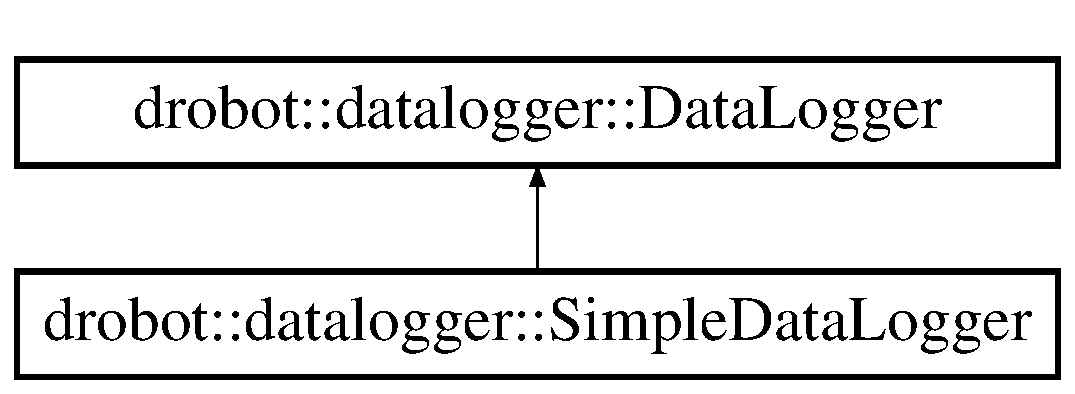
\includegraphics[height=3.000000cm]{classdrobot_1_1datalogger_1_1DataLogger}
\end{center}
\end{figure}
\subsection*{Public Member Functions}
\begin{DoxyCompactItemize}
\item 
\hypertarget{classdrobot_1_1datalogger_1_1DataLogger_ad7afd9487ac37f503ebe9159872a79dc}{{\bfseries Data\-Logger} (std\-::vector$<$ \hyperlink{classdrobot_1_1device_1_1channel_1_1Channel}{device\-::channel\-::\-Channel} $\ast$ $>$ channels)}\label{classdrobot_1_1datalogger_1_1DataLogger_ad7afd9487ac37f503ebe9159872a79dc}

\item 
virtual void \hyperlink{classdrobot_1_1datalogger_1_1DataLogger_a830fcb8f0b8b261bba22cfce46f4d309}{on\-Event} (\hyperlink{classdrobot_1_1event_1_1Event}{event\-::\-Event} $\ast$event)
\begin{DoxyCompactList}\small\item\em on\-Event. This method is called when an event of this type is fired. \end{DoxyCompactList}\item 
\hypertarget{classdrobot_1_1datalogger_1_1DataLogger_a96749bea55223e65aa2857dd9582f5ee}{std\-::vector\\*
$<$ \hyperlink{classdrobot_1_1device_1_1channel_1_1Channel}{device\-::channel\-::\-Channel} $\ast$ $>$ {\bfseries get\-Channels} ()}\label{classdrobot_1_1datalogger_1_1DataLogger_a96749bea55223e65aa2857dd9582f5ee}

\item 
\hypertarget{classdrobot_1_1datalogger_1_1DataLogger_a18e98de85b473a1e44e6f6793417b7b2}{virtual void {\bfseries log} (long tick, std\-::map$<$ \hyperlink{classdrobot_1_1device_1_1channel_1_1Channel}{device\-::channel\-::\-Channel} $\ast$, double $>$ values)}\label{classdrobot_1_1datalogger_1_1DataLogger_a18e98de85b473a1e44e6f6793417b7b2}

\item 
virtual void \hyperlink{classdrobot_1_1datalogger_1_1DataLogger_ae90262e477952f8e1c385b84e17d80c6}{set\-Max\-Values} (int max\-Values)=0
\begin{DoxyCompactList}\small\item\em set\-Max\-Values. max count of values. \end{DoxyCompactList}\item 
virtual int \hyperlink{classdrobot_1_1datalogger_1_1DataLogger_a8fe7bb2a626d9f9d5c69f9197490515b}{get\-Max\-Values} ()=0
\begin{DoxyCompactList}\small\item\em get\-Max\-Values. max count of values. \end{DoxyCompactList}\item 
virtual void \hyperlink{classdrobot_1_1datalogger_1_1DataLogger_ae463aebd8cb38c716bef83d5732042b1}{set\-Modulo} (int modulo)=0
\begin{DoxyCompactList}\small\item\em set\-Modulo. which ticks are recorded \end{DoxyCompactList}\item 
virtual int \hyperlink{classdrobot_1_1datalogger_1_1DataLogger_a4dd79d4060e4d4d77451a50777792c0a}{get\-Modulo} ()=0
\begin{DoxyCompactList}\small\item\em get\-Modulo. which ticks are recorded \end{DoxyCompactList}\end{DoxyCompactItemize}
\subsection*{Protected Attributes}
\begin{DoxyCompactItemize}
\item 
\hypertarget{classdrobot_1_1datalogger_1_1DataLogger_a9b2db99bfd6f3b640d1a8f96c9fd9da0}{std\-::vector\\*
$<$ \hyperlink{classdrobot_1_1device_1_1channel_1_1Channel}{device\-::channel\-::\-Channel} $\ast$ $>$ {\bfseries \-\_\-channels}}\label{classdrobot_1_1datalogger_1_1DataLogger_a9b2db99bfd6f3b640d1a8f96c9fd9da0}

\end{DoxyCompactItemize}


\subsection{Detailed Description}
The \hyperlink{classdrobot_1_1datalogger_1_1DataLogger}{Data\-Logger} class is a base class for collecting data from the robot. 

\subsection{Member Function Documentation}
\hypertarget{classdrobot_1_1datalogger_1_1DataLogger_a8fe7bb2a626d9f9d5c69f9197490515b}{\index{drobot\-::datalogger\-::\-Data\-Logger@{drobot\-::datalogger\-::\-Data\-Logger}!get\-Max\-Values@{get\-Max\-Values}}
\index{get\-Max\-Values@{get\-Max\-Values}!drobot::datalogger::DataLogger@{drobot\-::datalogger\-::\-Data\-Logger}}
\subsubsection[{get\-Max\-Values}]{\setlength{\rightskip}{0pt plus 5cm}virtual int drobot\-::datalogger\-::\-Data\-Logger\-::get\-Max\-Values (
\begin{DoxyParamCaption}
{}
\end{DoxyParamCaption}
)\hspace{0.3cm}{\ttfamily [pure virtual]}}}\label{classdrobot_1_1datalogger_1_1DataLogger_a8fe7bb2a626d9f9d5c69f9197490515b}


get\-Max\-Values. max count of values. 

If bigger than 0 the values from the oldest ticks are deleted so that the size doesn't exceeds max\-Values \begin{DoxyReturn}{Returns}
max\-Values 
\end{DoxyReturn}


Implemented in \hyperlink{classdrobot_1_1datalogger_1_1SimpleDataLogger_a2b9a75d2f73bb22e6558166e9dbcc4f4}{drobot\-::datalogger\-::\-Simple\-Data\-Logger}.

\hypertarget{classdrobot_1_1datalogger_1_1DataLogger_a4dd79d4060e4d4d77451a50777792c0a}{\index{drobot\-::datalogger\-::\-Data\-Logger@{drobot\-::datalogger\-::\-Data\-Logger}!get\-Modulo@{get\-Modulo}}
\index{get\-Modulo@{get\-Modulo}!drobot::datalogger::DataLogger@{drobot\-::datalogger\-::\-Data\-Logger}}
\subsubsection[{get\-Modulo}]{\setlength{\rightskip}{0pt plus 5cm}virtual int drobot\-::datalogger\-::\-Data\-Logger\-::get\-Modulo (
\begin{DoxyParamCaption}
{}
\end{DoxyParamCaption}
)\hspace{0.3cm}{\ttfamily [pure virtual]}}}\label{classdrobot_1_1datalogger_1_1DataLogger_a4dd79d4060e4d4d77451a50777792c0a}


get\-Modulo. which ticks are recorded 

if bigger than 0 only ticks with (tick \% module == 0) are recorded \begin{DoxyReturn}{Returns}
modulo 
\end{DoxyReturn}


Implemented in \hyperlink{classdrobot_1_1datalogger_1_1SimpleDataLogger_a43d243494d611d7f1c6afd5204686f40}{drobot\-::datalogger\-::\-Simple\-Data\-Logger}.

\hypertarget{classdrobot_1_1datalogger_1_1DataLogger_a830fcb8f0b8b261bba22cfce46f4d309}{\index{drobot\-::datalogger\-::\-Data\-Logger@{drobot\-::datalogger\-::\-Data\-Logger}!on\-Event@{on\-Event}}
\index{on\-Event@{on\-Event}!drobot::datalogger::DataLogger@{drobot\-::datalogger\-::\-Data\-Logger}}
\subsubsection[{on\-Event}]{\setlength{\rightskip}{0pt plus 5cm}void drobot\-::datalogger\-::\-Data\-Logger\-::on\-Event (
\begin{DoxyParamCaption}
\item[{{\bf event\-::\-Event} $\ast$}]{event}
\end{DoxyParamCaption}
)\hspace{0.3cm}{\ttfamily [virtual]}}}\label{classdrobot_1_1datalogger_1_1DataLogger_a830fcb8f0b8b261bba22cfce46f4d309}


on\-Event. This method is called when an event of this type is fired. 


\begin{DoxyParams}{Parameters}
{\em event} & fired \\
\hline
\end{DoxyParams}


Implements \hyperlink{classdrobot_1_1event_1_1EventListener_ae5e30e4a518f6752a09f44f8dc6cdc51}{drobot\-::event\-::\-Event\-Listener}.

\hypertarget{classdrobot_1_1datalogger_1_1DataLogger_ae90262e477952f8e1c385b84e17d80c6}{\index{drobot\-::datalogger\-::\-Data\-Logger@{drobot\-::datalogger\-::\-Data\-Logger}!set\-Max\-Values@{set\-Max\-Values}}
\index{set\-Max\-Values@{set\-Max\-Values}!drobot::datalogger::DataLogger@{drobot\-::datalogger\-::\-Data\-Logger}}
\subsubsection[{set\-Max\-Values}]{\setlength{\rightskip}{0pt plus 5cm}virtual void drobot\-::datalogger\-::\-Data\-Logger\-::set\-Max\-Values (
\begin{DoxyParamCaption}
\item[{int}]{max\-Values}
\end{DoxyParamCaption}
)\hspace{0.3cm}{\ttfamily [pure virtual]}}}\label{classdrobot_1_1datalogger_1_1DataLogger_ae90262e477952f8e1c385b84e17d80c6}


set\-Max\-Values. max count of values. 

If bigger than 0 the values from the oldest ticks are deleted so that the size doesn't exceeds max\-Values 
\begin{DoxyParams}{Parameters}
{\em max\-Values} & \\
\hline
\end{DoxyParams}


Implemented in \hyperlink{classdrobot_1_1datalogger_1_1SimpleDataLogger_a8e79821846b2104d7f65e64f6e8a5eb6}{drobot\-::datalogger\-::\-Simple\-Data\-Logger}.

\hypertarget{classdrobot_1_1datalogger_1_1DataLogger_ae463aebd8cb38c716bef83d5732042b1}{\index{drobot\-::datalogger\-::\-Data\-Logger@{drobot\-::datalogger\-::\-Data\-Logger}!set\-Modulo@{set\-Modulo}}
\index{set\-Modulo@{set\-Modulo}!drobot::datalogger::DataLogger@{drobot\-::datalogger\-::\-Data\-Logger}}
\subsubsection[{set\-Modulo}]{\setlength{\rightskip}{0pt plus 5cm}virtual void drobot\-::datalogger\-::\-Data\-Logger\-::set\-Modulo (
\begin{DoxyParamCaption}
\item[{int}]{modulo}
\end{DoxyParamCaption}
)\hspace{0.3cm}{\ttfamily [pure virtual]}}}\label{classdrobot_1_1datalogger_1_1DataLogger_ae463aebd8cb38c716bef83d5732042b1}


set\-Modulo. which ticks are recorded 

if bigger than 0 only ticks with (tick \% module == 0) are recorded 
\begin{DoxyParams}{Parameters}
{\em modulo} & \\
\hline
\end{DoxyParams}


Implemented in \hyperlink{classdrobot_1_1datalogger_1_1SimpleDataLogger_a4365669efc4d0950cf21c30be8650a88}{drobot\-::datalogger\-::\-Simple\-Data\-Logger}.



The documentation for this class was generated from the following files\-:\begin{DoxyCompactItemize}
\item 
/home/imanol/workspace/drobot/new/src/drobot/datalogger/datalogger.\-h\item 
/home/imanol/workspace/drobot/new/src/drobot/datalogger/datalogger.\-cpp\end{DoxyCompactItemize}

\hypertarget{classdrobot_1_1device_1_1Device}{\section{drobot\-:\-:device\-:\-:Device Class Reference}
\label{classdrobot_1_1device_1_1Device}\index{drobot\-::device\-::\-Device@{drobot\-::device\-::\-Device}}
}


Represents a physical or virtual (simulated) device.  




{\ttfamily \#include $<$device.\-h$>$}

Inheritance diagram for drobot\-:\-:device\-:\-:Device\-:\begin{figure}[H]
\begin{center}
\leavevmode
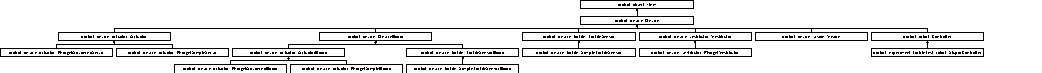
\includegraphics[height=0.981423cm]{classdrobot_1_1device_1_1Device}
\end{center}
\end{figure}
\subsection*{Public Member Functions}
\begin{DoxyCompactItemize}
\item 
\hypertarget{classdrobot_1_1device_1_1Device_ab55bd66f79422bd251ea5f94e80ba036}{{\bfseries Device} (std\-::string name)}\label{classdrobot_1_1device_1_1Device_ab55bd66f79422bd251ea5f94e80ba036}

\item 
virtual void \hyperlink{classdrobot_1_1device_1_1Device_a0c28785ff2e79f99b8e9eaefe6749f2b}{enable} ()
\begin{DoxyCompactList}\small\item\em enables the device. \end{DoxyCompactList}\item 
virtual void \hyperlink{classdrobot_1_1device_1_1Device_a289499673ae30bd72101c68fbd04cd89}{disable} ()
\begin{DoxyCompactList}\small\item\em disables the device. \end{DoxyCompactList}\item 
virtual bool \hyperlink{classdrobot_1_1device_1_1Device_aa5b7eac8638d0d2d5ee9bf10607b100e}{is\-Enabled} ()=0
\begin{DoxyCompactList}\small\item\em check if the device is enabled \end{DoxyCompactList}\item 
\hyperlink{classdrobot_1_1device_1_1DeviceBoard}{Device\-Board} $\ast$ \hyperlink{classdrobot_1_1device_1_1Device_abb2094b9cb9a794eb9c8c9798b37a376}{get\-Device\-Board} ()
\item 
void \hyperlink{classdrobot_1_1device_1_1Device_a60464a906ee599de5d4368a373a368d3}{set\-Device\-Board} (\hyperlink{classdrobot_1_1device_1_1DeviceBoard}{Device\-Board} $\ast$device\-Board)
\begin{DoxyCompactList}\small\item\em sets the \hyperlink{classdrobot_1_1device_1_1DeviceBoard}{Device\-Board} \end{DoxyCompactList}\item 
\hyperlink{classdrobot_1_1device_1_1Device}{Device} $\ast$ \hyperlink{classdrobot_1_1device_1_1Device_a2ad010960f753e0299afae8c89708d34}{to\-Device} ()
\begin{DoxyCompactList}\small\item\em cast to \hyperlink{classdrobot_1_1device_1_1Device}{Device} \end{DoxyCompactList}\item 
\hyperlink{classdrobot_1_1device_1_1actuator_1_1Actuator}{actuator\-::\-Actuator} $\ast$ \hyperlink{classdrobot_1_1device_1_1Device_a4aa4ad98eb5ed0251fa48b6ebd5c96d6}{to\-Actuator} ()
\begin{DoxyCompactList}\small\item\em cast to \hyperlink{classdrobot_1_1device_1_1actuator_1_1Actuator}{actuator\-::\-Actuator} \end{DoxyCompactList}\item 
\hyperlink{classdrobot_1_1device_1_1tactile_1_1TactileSensor}{tactile\-::\-Tactile\-Sensor} $\ast$ \hyperlink{classdrobot_1_1device_1_1Device_a2f95e9596d7fa2dffcf2e398192d46c0}{to\-Tactile\-Sensor} ()
\begin{DoxyCompactList}\small\item\em cast to \hyperlink{classdrobot_1_1device_1_1tactile_1_1TactileSensor}{tactile\-::\-Tactile\-Sensor} \end{DoxyCompactList}\item 
\hyperlink{classdrobot_1_1device_1_1vestibular_1_1Vestibular}{vestibular\-::\-Vestibular} $\ast$ \hyperlink{classdrobot_1_1device_1_1Device_a3ad656dee133fa5df9eaa466b3530234}{to\-Vestibular} ()
\begin{DoxyCompactList}\small\item\em cast to \hyperlink{classdrobot_1_1device_1_1vestibular_1_1Vestibular}{vestibular\-::\-Vestibular} \end{DoxyCompactList}\item 
\hyperlink{classdrobot_1_1device_1_1vision_1_1Vision}{vision\-::\-Vision} $\ast$ \hyperlink{classdrobot_1_1device_1_1Device_a7041c41a60a8eccd694ff08c0a8f5827}{to\-Vision} ()
\begin{DoxyCompactList}\small\item\em cast to \hyperlink{classdrobot_1_1device_1_1vision_1_1Vision}{vision\-::\-Vision} \end{DoxyCompactList}\item 
virtual \hyperlink{classdrobot_1_1device_1_1channel_1_1ChannelManager}{channel\-::\-Channel\-Manager} $\ast$ \hyperlink{classdrobot_1_1device_1_1Device_a67e466715422618b28226a17f14c0170}{get\-Channels} ()
\end{DoxyCompactItemize}
\subsection*{Private Attributes}
\begin{DoxyCompactItemize}
\item 
\hypertarget{classdrobot_1_1device_1_1Device_abb3a110d904ae7de3abae5415fc273a3}{\hyperlink{classdrobot_1_1device_1_1DeviceBoard}{Device\-Board} $\ast$ \hyperlink{classdrobot_1_1device_1_1Device_abb3a110d904ae7de3abae5415fc273a3}{\-\_\-device\-Board}}\label{classdrobot_1_1device_1_1Device_abb3a110d904ae7de3abae5415fc273a3}

\begin{DoxyCompactList}\small\item\em \-\_\-device\-Board The \hyperlink{classdrobot_1_1device_1_1DeviceBoard}{Device\-Board} it belongs to \end{DoxyCompactList}\item 
\hypertarget{classdrobot_1_1device_1_1Device_a3f909e61d1a8e821aa57cc12291ef1a9}{\hyperlink{classdrobot_1_1device_1_1channel_1_1ChannelManager}{channel\-::\-Channel\-Manager} $\ast$ \hyperlink{classdrobot_1_1device_1_1Device_a3f909e61d1a8e821aa57cc12291ef1a9}{\-\_\-channels}}\label{classdrobot_1_1device_1_1Device_a3f909e61d1a8e821aa57cc12291ef1a9}

\begin{DoxyCompactList}\small\item\em \-\_\-channels Data structure containing the channels \end{DoxyCompactList}\end{DoxyCompactItemize}
\subsection*{Additional Inherited Members}


\subsection{Detailed Description}
Represents a physical or virtual (simulated) device. 

A device can be any part of a robot actuator or sensor. It can also be used to implement a virtual device like a robot controller for instance. A device contains different kinds of channels represented by the \hyperlink{classdrobot_1_1device_1_1channel_1_1Channel}{drobot\-::device\-::channel\-::\-Channel} class which are managed by the \-\_\-channels property. To add and remove channels use the \-\_\-channels property (See \hyperlink{classdrobot_1_1object_1_1Manager}{object\-::\-Manager}). Certain devices belong to a \hyperlink{classdrobot_1_1device_1_1DeviceBoard}{Device\-Board} (See \hyperlink{classdrobot_1_1device_1_1actuator_1_1PhidgetAdvancedServo}{actuator\-::\-Phidget\-Advanced\-Servo} for example). 

\subsection{Member Function Documentation}
\hypertarget{classdrobot_1_1device_1_1Device_a289499673ae30bd72101c68fbd04cd89}{\index{drobot\-::device\-::\-Device@{drobot\-::device\-::\-Device}!disable@{disable}}
\index{disable@{disable}!drobot::device::Device@{drobot\-::device\-::\-Device}}
\subsubsection[{disable}]{\setlength{\rightskip}{0pt plus 5cm}void drobot\-::device\-::\-Device\-::disable (
\begin{DoxyParamCaption}
{}
\end{DoxyParamCaption}
)\hspace{0.3cm}{\ttfamily [virtual]}}}\label{classdrobot_1_1device_1_1Device_a289499673ae30bd72101c68fbd04cd89}


disables the device. 

This function has to be implemented by the specific device. For physical devices like actuators this method should power off the device; 

Reimplemented in \hyperlink{classdrobot_1_1device_1_1vestibular_1_1PhidgetVestibular_ae1887d6d36bf2a25925663e35bd6d57d}{drobot\-::device\-::vestibular\-::\-Phidget\-Vestibular}, \hyperlink{classdrobot_1_1robot_1_1Controller_a40384f970deab8157ada1ead78d8b383}{drobot\-::robot\-::\-Controller}, \hyperlink{classdrobot_1_1device_1_1tactile_1_1SimpleTactileSensor_a0599c06afdb09494de0e6756a878cbad}{drobot\-::device\-::tactile\-::\-Simple\-Tactile\-Sensor}, \hyperlink{classdrobot_1_1device_1_1actuator_1_1PhidgetSimpleServo_ad3dffbddc718a4f447a75bc90c0cb8f1}{drobot\-::device\-::actuator\-::\-Phidget\-Simple\-Servo}, \hyperlink{classdrobot_1_1device_1_1actuator_1_1PhidgetAdvancedServo_a62ef62d1c2052af2f2b2db1443e21c1b}{drobot\-::device\-::actuator\-::\-Phidget\-Advanced\-Servo}, and \hyperlink{classdrobot_1_1device_1_1DeviceBoard_a65eb028173bd7308192f1781d18f292d}{drobot\-::device\-::\-Device\-Board}.

\hypertarget{classdrobot_1_1device_1_1Device_a0c28785ff2e79f99b8e9eaefe6749f2b}{\index{drobot\-::device\-::\-Device@{drobot\-::device\-::\-Device}!enable@{enable}}
\index{enable@{enable}!drobot::device::Device@{drobot\-::device\-::\-Device}}
\subsubsection[{enable}]{\setlength{\rightskip}{0pt plus 5cm}void drobot\-::device\-::\-Device\-::enable (
\begin{DoxyParamCaption}
{}
\end{DoxyParamCaption}
)\hspace{0.3cm}{\ttfamily [virtual]}}}\label{classdrobot_1_1device_1_1Device_a0c28785ff2e79f99b8e9eaefe6749f2b}


enables the device. 

This function has to be implemented by the specific device. For physical devices like actuators this method should power on the device. 

Reimplemented in \hyperlink{classdrobot_1_1device_1_1vestibular_1_1PhidgetVestibular_a23ef10594aaaddb5f3f2a9908b531c23}{drobot\-::device\-::vestibular\-::\-Phidget\-Vestibular}, \hyperlink{classdrobot_1_1robot_1_1Controller_a533a9761503d502c64c25538ce8eb35c}{drobot\-::robot\-::\-Controller}, \hyperlink{classdrobot_1_1device_1_1tactile_1_1SimpleTactileSensor_a006318b86b569b7f72605d24f1948042}{drobot\-::device\-::tactile\-::\-Simple\-Tactile\-Sensor}, \hyperlink{classdrobot_1_1device_1_1actuator_1_1PhidgetSimpleServo_ada2b985fee1f6a3891effad83fb7f738}{drobot\-::device\-::actuator\-::\-Phidget\-Simple\-Servo}, \hyperlink{classdrobot_1_1device_1_1actuator_1_1PhidgetAdvancedServo_aff32b9715c9095ed27b8b6268706b778}{drobot\-::device\-::actuator\-::\-Phidget\-Advanced\-Servo}, \hyperlink{classdrobot_1_1device_1_1DeviceBoard_a1a01810b04372666baaafaf812e5a54e}{drobot\-::device\-::\-Device\-Board}, and \hyperlink{classdrobot_1_1device_1_1tactile_1_1SimpleTactileSensorBoard_a1660e1e8cd1d5705936a28ce9294d759}{drobot\-::device\-::tactile\-::\-Simple\-Tactile\-Sensor\-Board}.

\hypertarget{classdrobot_1_1device_1_1Device_a67e466715422618b28226a17f14c0170}{\index{drobot\-::device\-::\-Device@{drobot\-::device\-::\-Device}!get\-Channels@{get\-Channels}}
\index{get\-Channels@{get\-Channels}!drobot::device::Device@{drobot\-::device\-::\-Device}}
\subsubsection[{get\-Channels}]{\setlength{\rightskip}{0pt plus 5cm}{\bf channel\-::\-Channel\-Manager} $\ast$ drobot\-::device\-::\-Device\-::get\-Channels (
\begin{DoxyParamCaption}
{}
\end{DoxyParamCaption}
)\hspace{0.3cm}{\ttfamily [virtual]}}}\label{classdrobot_1_1device_1_1Device_a67e466715422618b28226a17f14c0170}
\begin{DoxyReturn}{Returns}
Data structure containing the devices channels. 
\end{DoxyReturn}


Reimplemented in \hyperlink{classdrobot_1_1device_1_1DeviceBoard_ad62ff708f54468e97d2ba46c96b67960}{drobot\-::device\-::\-Device\-Board}.

\hypertarget{classdrobot_1_1device_1_1Device_abb2094b9cb9a794eb9c8c9798b37a376}{\index{drobot\-::device\-::\-Device@{drobot\-::device\-::\-Device}!get\-Device\-Board@{get\-Device\-Board}}
\index{get\-Device\-Board@{get\-Device\-Board}!drobot::device::Device@{drobot\-::device\-::\-Device}}
\subsubsection[{get\-Device\-Board}]{\setlength{\rightskip}{0pt plus 5cm}{\bf Device\-Board} $\ast$ drobot\-::device\-::\-Device\-::get\-Device\-Board (
\begin{DoxyParamCaption}
{}
\end{DoxyParamCaption}
)}}\label{classdrobot_1_1device_1_1Device_abb2094b9cb9a794eb9c8c9798b37a376}
\begin{DoxyReturn}{Returns}
the \hyperlink{classdrobot_1_1device_1_1DeviceBoard}{Device\-Board} 
\end{DoxyReturn}
\hypertarget{classdrobot_1_1device_1_1Device_aa5b7eac8638d0d2d5ee9bf10607b100e}{\index{drobot\-::device\-::\-Device@{drobot\-::device\-::\-Device}!is\-Enabled@{is\-Enabled}}
\index{is\-Enabled@{is\-Enabled}!drobot::device::Device@{drobot\-::device\-::\-Device}}
\subsubsection[{is\-Enabled}]{\setlength{\rightskip}{0pt plus 5cm}virtual bool drobot\-::device\-::\-Device\-::is\-Enabled (
\begin{DoxyParamCaption}
{}
\end{DoxyParamCaption}
)\hspace{0.3cm}{\ttfamily [pure virtual]}}}\label{classdrobot_1_1device_1_1Device_aa5b7eac8638d0d2d5ee9bf10607b100e}


check if the device is enabled 

\begin{DoxyReturn}{Returns}
true if enabled else false
\end{DoxyReturn}
While the \hyperlink{classdrobot_1_1robot_1_1Robot}{drobot\-::robot\-::\-Robot} is running this property is checked to see whether the device should be used or not. 

Implemented in \hyperlink{classdrobot_1_1device_1_1vestibular_1_1PhidgetVestibular_aed99fc288425612c447cc0df4938d9cd}{drobot\-::device\-::vestibular\-::\-Phidget\-Vestibular}, \hyperlink{classdrobot_1_1robot_1_1Controller_a8f7c73ba2adb3f7c02ff97b5c9d94b12}{drobot\-::robot\-::\-Controller}, \hyperlink{classdrobot_1_1device_1_1tactile_1_1SimpleTactileSensor_a54b5ab7b69bb3b15727ef72143799f34}{drobot\-::device\-::tactile\-::\-Simple\-Tactile\-Sensor}, \hyperlink{classdrobot_1_1device_1_1actuator_1_1PhidgetSimpleServo_a6da8b37b613ecf9c8fc12f335ec90537}{drobot\-::device\-::actuator\-::\-Phidget\-Simple\-Servo}, \hyperlink{classdrobot_1_1device_1_1actuator_1_1PhidgetAdvancedServo_aaae782fc07c5fea70969560713c36d8c}{drobot\-::device\-::actuator\-::\-Phidget\-Advanced\-Servo}, and \hyperlink{classdrobot_1_1device_1_1DeviceBoard_a23bae9f0c7f099bbb5f0c696ff5c126a}{drobot\-::device\-::\-Device\-Board}.

\hypertarget{classdrobot_1_1device_1_1Device_a60464a906ee599de5d4368a373a368d3}{\index{drobot\-::device\-::\-Device@{drobot\-::device\-::\-Device}!set\-Device\-Board@{set\-Device\-Board}}
\index{set\-Device\-Board@{set\-Device\-Board}!drobot::device::Device@{drobot\-::device\-::\-Device}}
\subsubsection[{set\-Device\-Board}]{\setlength{\rightskip}{0pt plus 5cm}void drobot\-::device\-::\-Device\-::set\-Device\-Board (
\begin{DoxyParamCaption}
\item[{{\bf Device\-Board} $\ast$}]{device\-Board}
\end{DoxyParamCaption}
)}}\label{classdrobot_1_1device_1_1Device_a60464a906ee599de5d4368a373a368d3}


sets the \hyperlink{classdrobot_1_1device_1_1DeviceBoard}{Device\-Board} 


\begin{DoxyParams}{Parameters}
{\em device\-Board} & \\
\hline
\end{DoxyParams}
\hypertarget{classdrobot_1_1device_1_1Device_a4aa4ad98eb5ed0251fa48b6ebd5c96d6}{\index{drobot\-::device\-::\-Device@{drobot\-::device\-::\-Device}!to\-Actuator@{to\-Actuator}}
\index{to\-Actuator@{to\-Actuator}!drobot::device::Device@{drobot\-::device\-::\-Device}}
\subsubsection[{to\-Actuator}]{\setlength{\rightskip}{0pt plus 5cm}{\bf actuator\-::\-Actuator} $\ast$ drobot\-::device\-::\-Device\-::to\-Actuator (
\begin{DoxyParamCaption}
{}
\end{DoxyParamCaption}
)}}\label{classdrobot_1_1device_1_1Device_a4aa4ad98eb5ed0251fa48b6ebd5c96d6}


cast to \hyperlink{classdrobot_1_1device_1_1actuator_1_1Actuator}{actuator\-::\-Actuator} 

\begin{DoxyReturn}{Returns}
\hyperlink{classdrobot_1_1device_1_1actuator_1_1Actuator}{actuator\-::\-Actuator} Pointer 
\end{DoxyReturn}
\hypertarget{classdrobot_1_1device_1_1Device_a2ad010960f753e0299afae8c89708d34}{\index{drobot\-::device\-::\-Device@{drobot\-::device\-::\-Device}!to\-Device@{to\-Device}}
\index{to\-Device@{to\-Device}!drobot::device::Device@{drobot\-::device\-::\-Device}}
\subsubsection[{to\-Device}]{\setlength{\rightskip}{0pt plus 5cm}{\bf Device} $\ast$ drobot\-::device\-::\-Device\-::to\-Device (
\begin{DoxyParamCaption}
{}
\end{DoxyParamCaption}
)}}\label{classdrobot_1_1device_1_1Device_a2ad010960f753e0299afae8c89708d34}


cast to \hyperlink{classdrobot_1_1device_1_1Device}{Device} 

\begin{DoxyReturn}{Returns}
\hyperlink{classdrobot_1_1device_1_1Device}{Device} Pointer 
\end{DoxyReturn}
\hypertarget{classdrobot_1_1device_1_1Device_a2f95e9596d7fa2dffcf2e398192d46c0}{\index{drobot\-::device\-::\-Device@{drobot\-::device\-::\-Device}!to\-Tactile\-Sensor@{to\-Tactile\-Sensor}}
\index{to\-Tactile\-Sensor@{to\-Tactile\-Sensor}!drobot::device::Device@{drobot\-::device\-::\-Device}}
\subsubsection[{to\-Tactile\-Sensor}]{\setlength{\rightskip}{0pt plus 5cm}{\bf tactile\-::\-Tactile\-Sensor} $\ast$ drobot\-::device\-::\-Device\-::to\-Tactile\-Sensor (
\begin{DoxyParamCaption}
{}
\end{DoxyParamCaption}
)}}\label{classdrobot_1_1device_1_1Device_a2f95e9596d7fa2dffcf2e398192d46c0}


cast to \hyperlink{classdrobot_1_1device_1_1tactile_1_1TactileSensor}{tactile\-::\-Tactile\-Sensor} 

\begin{DoxyReturn}{Returns}
\hyperlink{classdrobot_1_1device_1_1tactile_1_1TactileSensor}{tactile\-::\-Tactile\-Sensor} Pointer 
\end{DoxyReturn}
\hypertarget{classdrobot_1_1device_1_1Device_a3ad656dee133fa5df9eaa466b3530234}{\index{drobot\-::device\-::\-Device@{drobot\-::device\-::\-Device}!to\-Vestibular@{to\-Vestibular}}
\index{to\-Vestibular@{to\-Vestibular}!drobot::device::Device@{drobot\-::device\-::\-Device}}
\subsubsection[{to\-Vestibular}]{\setlength{\rightskip}{0pt plus 5cm}{\bf vestibular\-::\-Vestibular} $\ast$ drobot\-::device\-::\-Device\-::to\-Vestibular (
\begin{DoxyParamCaption}
{}
\end{DoxyParamCaption}
)}}\label{classdrobot_1_1device_1_1Device_a3ad656dee133fa5df9eaa466b3530234}


cast to \hyperlink{classdrobot_1_1device_1_1vestibular_1_1Vestibular}{vestibular\-::\-Vestibular} 

\begin{DoxyReturn}{Returns}
\hyperlink{classdrobot_1_1device_1_1vestibular_1_1Vestibular}{vestibular\-::\-Vestibular} Pointer 
\end{DoxyReturn}
\hypertarget{classdrobot_1_1device_1_1Device_a7041c41a60a8eccd694ff08c0a8f5827}{\index{drobot\-::device\-::\-Device@{drobot\-::device\-::\-Device}!to\-Vision@{to\-Vision}}
\index{to\-Vision@{to\-Vision}!drobot::device::Device@{drobot\-::device\-::\-Device}}
\subsubsection[{to\-Vision}]{\setlength{\rightskip}{0pt plus 5cm}{\bf vision\-::\-Vision}$\ast$ drobot\-::device\-::\-Device\-::to\-Vision (
\begin{DoxyParamCaption}
{}
\end{DoxyParamCaption}
)}}\label{classdrobot_1_1device_1_1Device_a7041c41a60a8eccd694ff08c0a8f5827}


cast to \hyperlink{classdrobot_1_1device_1_1vision_1_1Vision}{vision\-::\-Vision} 

\begin{DoxyReturn}{Returns}
\hyperlink{classdrobot_1_1device_1_1vision_1_1Vision}{vision\-::\-Vision} Pointer 
\end{DoxyReturn}


The documentation for this class was generated from the following files\-:\begin{DoxyCompactItemize}
\item 
/home/imanol/workspace/drobot/new/src/drobot/device/device.\-h\item 
/home/imanol/workspace/drobot/new/src/drobot/device/device.\-cpp\end{DoxyCompactItemize}

\hypertarget{classdrobot_1_1device_1_1DeviceBoard}{\section{drobot\-:\-:device\-:\-:Device\-Board Class Reference}
\label{classdrobot_1_1device_1_1DeviceBoard}\index{drobot\-::device\-::\-Device\-Board@{drobot\-::device\-::\-Device\-Board}}
}


Represents a board with devices plugged into it.  




{\ttfamily \#include $<$deviceboard.\-h$>$}

Inheritance diagram for drobot\-:\-:device\-:\-:Device\-Board\-:\begin{figure}[H]
\begin{center}
\leavevmode
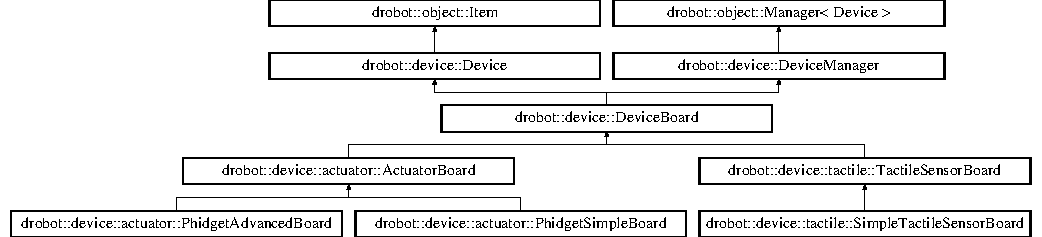
\includegraphics[height=3.185438cm]{classdrobot_1_1device_1_1DeviceBoard}
\end{center}
\end{figure}
\subsection*{Public Member Functions}
\begin{DoxyCompactItemize}
\item 
\hypertarget{classdrobot_1_1device_1_1DeviceBoard_a09e11fda1665667f2f765a6f1acaaecb}{{\bfseries Device\-Board} (std\-::string name)}\label{classdrobot_1_1device_1_1DeviceBoard_a09e11fda1665667f2f765a6f1acaaecb}

\item 
virtual void \hyperlink{classdrobot_1_1device_1_1DeviceBoard_a1a01810b04372666baaafaf812e5a54e}{enable} ()
\begin{DoxyCompactList}\small\item\em enables the device. \end{DoxyCompactList}\item 
virtual void \hyperlink{classdrobot_1_1device_1_1DeviceBoard_a65eb028173bd7308192f1781d18f292d}{disable} ()
\begin{DoxyCompactList}\small\item\em disables the device. \end{DoxyCompactList}\item 
virtual bool \hyperlink{classdrobot_1_1device_1_1DeviceBoard_a23bae9f0c7f099bbb5f0c696ff5c126a}{is\-Enabled} ()
\begin{DoxyCompactList}\small\item\em check if the device is enabled \end{DoxyCompactList}\item 
virtual void \hyperlink{classdrobot_1_1device_1_1DeviceBoard_a51c658f37640d901e2ecaf6a612eaa15}{on\-Add} (\hyperlink{classdrobot_1_1device_1_1Device}{Device} $\ast$item)
\begin{DoxyCompactList}\small\item\em this method is called every time a device is added. It automatically adds the devices channels to the \hyperlink{classdrobot_1_1device_1_1channel_1_1ChannelManager}{channel\-::\-Channel\-Manager} and sets the reverse dependency on the device to this. \end{DoxyCompactList}\item 
virtual void \hyperlink{classdrobot_1_1device_1_1DeviceBoard_ab42d2d02abc3593960a9d6c18facf36e}{on\-Remove} (\hyperlink{classdrobot_1_1device_1_1Device}{Device} $\ast$item)
\begin{DoxyCompactList}\small\item\em this method is called every time a device is removed. It automatically removes the devices channels from the \hyperlink{classdrobot_1_1device_1_1channel_1_1ChannelManager}{channel\-::\-Channel\-Manager} and sets the reverse dependency on the device to 0. \end{DoxyCompactList}\item 
virtual \hyperlink{classdrobot_1_1device_1_1channel_1_1ChannelManager}{channel\-::\-Channel\-Manager} $\ast$ \hyperlink{classdrobot_1_1device_1_1DeviceBoard_ad62ff708f54468e97d2ba46c96b67960}{get\-Channels} ()
\end{DoxyCompactItemize}
\subsection*{Private Attributes}
\begin{DoxyCompactItemize}
\item 
\hypertarget{classdrobot_1_1device_1_1DeviceBoard_a03d1dfa32694561262a9589d607b7fca}{bool \hyperlink{classdrobot_1_1device_1_1DeviceBoard_a03d1dfa32694561262a9589d607b7fca}{\-\_\-enabled}}\label{classdrobot_1_1device_1_1DeviceBoard_a03d1dfa32694561262a9589d607b7fca}

\begin{DoxyCompactList}\small\item\em flag indicating whether it is enabled or not \end{DoxyCompactList}\end{DoxyCompactItemize}
\subsection*{Additional Inherited Members}


\subsection{Detailed Description}
Represents a board with devices plugged into it. 

This class should be used as a base class for Phidget boards etc. It can be treated as a device and also as a device manager. it also contains all the channels of the devices. 

\subsection{Member Function Documentation}
\hypertarget{classdrobot_1_1device_1_1DeviceBoard_a65eb028173bd7308192f1781d18f292d}{\index{drobot\-::device\-::\-Device\-Board@{drobot\-::device\-::\-Device\-Board}!disable@{disable}}
\index{disable@{disable}!drobot::device::DeviceBoard@{drobot\-::device\-::\-Device\-Board}}
\subsubsection[{disable}]{\setlength{\rightskip}{0pt plus 5cm}void drobot\-::device\-::\-Device\-Board\-::disable (
\begin{DoxyParamCaption}
{}
\end{DoxyParamCaption}
)\hspace{0.3cm}{\ttfamily [virtual]}}}\label{classdrobot_1_1device_1_1DeviceBoard_a65eb028173bd7308192f1781d18f292d}


disables the device. 

This function has to be implemented by the specific device. For physical devices like actuators this method should power off the device; 

Reimplemented from \hyperlink{classdrobot_1_1device_1_1Device_a289499673ae30bd72101c68fbd04cd89}{drobot\-::device\-::\-Device}.

\hypertarget{classdrobot_1_1device_1_1DeviceBoard_a1a01810b04372666baaafaf812e5a54e}{\index{drobot\-::device\-::\-Device\-Board@{drobot\-::device\-::\-Device\-Board}!enable@{enable}}
\index{enable@{enable}!drobot::device::DeviceBoard@{drobot\-::device\-::\-Device\-Board}}
\subsubsection[{enable}]{\setlength{\rightskip}{0pt plus 5cm}void drobot\-::device\-::\-Device\-Board\-::enable (
\begin{DoxyParamCaption}
{}
\end{DoxyParamCaption}
)\hspace{0.3cm}{\ttfamily [virtual]}}}\label{classdrobot_1_1device_1_1DeviceBoard_a1a01810b04372666baaafaf812e5a54e}


enables the device. 

This function has to be implemented by the specific device. For physical devices like actuators this method should power on the device. 

Reimplemented from \hyperlink{classdrobot_1_1device_1_1Device_a0c28785ff2e79f99b8e9eaefe6749f2b}{drobot\-::device\-::\-Device}.



Reimplemented in \hyperlink{classdrobot_1_1device_1_1tactile_1_1SimpleTactileSensorBoard_a1660e1e8cd1d5705936a28ce9294d759}{drobot\-::device\-::tactile\-::\-Simple\-Tactile\-Sensor\-Board}.

\hypertarget{classdrobot_1_1device_1_1DeviceBoard_ad62ff708f54468e97d2ba46c96b67960}{\index{drobot\-::device\-::\-Device\-Board@{drobot\-::device\-::\-Device\-Board}!get\-Channels@{get\-Channels}}
\index{get\-Channels@{get\-Channels}!drobot::device::DeviceBoard@{drobot\-::device\-::\-Device\-Board}}
\subsubsection[{get\-Channels}]{\setlength{\rightskip}{0pt plus 5cm}{\bf channel\-::\-Channel\-Manager} $\ast$ drobot\-::device\-::\-Device\-Board\-::get\-Channels (
\begin{DoxyParamCaption}
{}
\end{DoxyParamCaption}
)\hspace{0.3cm}{\ttfamily [virtual]}}}\label{classdrobot_1_1device_1_1DeviceBoard_ad62ff708f54468e97d2ba46c96b67960}
\begin{DoxyReturn}{Returns}
the channels of the Devices. 
\end{DoxyReturn}


Reimplemented from \hyperlink{classdrobot_1_1device_1_1Device_a67e466715422618b28226a17f14c0170}{drobot\-::device\-::\-Device}.

\hypertarget{classdrobot_1_1device_1_1DeviceBoard_a23bae9f0c7f099bbb5f0c696ff5c126a}{\index{drobot\-::device\-::\-Device\-Board@{drobot\-::device\-::\-Device\-Board}!is\-Enabled@{is\-Enabled}}
\index{is\-Enabled@{is\-Enabled}!drobot::device::DeviceBoard@{drobot\-::device\-::\-Device\-Board}}
\subsubsection[{is\-Enabled}]{\setlength{\rightskip}{0pt plus 5cm}bool drobot\-::device\-::\-Device\-Board\-::is\-Enabled (
\begin{DoxyParamCaption}
{}
\end{DoxyParamCaption}
)\hspace{0.3cm}{\ttfamily [virtual]}}}\label{classdrobot_1_1device_1_1DeviceBoard_a23bae9f0c7f099bbb5f0c696ff5c126a}


check if the device is enabled 

\begin{DoxyReturn}{Returns}
true if enabled else false
\end{DoxyReturn}
While the \hyperlink{classdrobot_1_1robot_1_1Robot}{drobot\-::robot\-::\-Robot} is running this property is checked to see whether the device should be used or not. 

Implements \hyperlink{classdrobot_1_1device_1_1Device_aa5b7eac8638d0d2d5ee9bf10607b100e}{drobot\-::device\-::\-Device}.

\hypertarget{classdrobot_1_1device_1_1DeviceBoard_a51c658f37640d901e2ecaf6a612eaa15}{\index{drobot\-::device\-::\-Device\-Board@{drobot\-::device\-::\-Device\-Board}!on\-Add@{on\-Add}}
\index{on\-Add@{on\-Add}!drobot::device::DeviceBoard@{drobot\-::device\-::\-Device\-Board}}
\subsubsection[{on\-Add}]{\setlength{\rightskip}{0pt plus 5cm}void drobot\-::device\-::\-Device\-Board\-::on\-Add (
\begin{DoxyParamCaption}
\item[{{\bf Device} $\ast$}]{item}
\end{DoxyParamCaption}
)\hspace{0.3cm}{\ttfamily [virtual]}}}\label{classdrobot_1_1device_1_1DeviceBoard_a51c658f37640d901e2ecaf6a612eaa15}


this method is called every time a device is added. It automatically adds the devices channels to the \hyperlink{classdrobot_1_1device_1_1channel_1_1ChannelManager}{channel\-::\-Channel\-Manager} and sets the reverse dependency on the device to this. 


\begin{DoxyParams}{Parameters}
{\em item} & \\
\hline
\end{DoxyParams}


Reimplemented from \hyperlink{classdrobot_1_1device_1_1DeviceManager}{drobot\-::device\-::\-Device\-Manager}.

\hypertarget{classdrobot_1_1device_1_1DeviceBoard_ab42d2d02abc3593960a9d6c18facf36e}{\index{drobot\-::device\-::\-Device\-Board@{drobot\-::device\-::\-Device\-Board}!on\-Remove@{on\-Remove}}
\index{on\-Remove@{on\-Remove}!drobot::device::DeviceBoard@{drobot\-::device\-::\-Device\-Board}}
\subsubsection[{on\-Remove}]{\setlength{\rightskip}{0pt plus 5cm}void drobot\-::device\-::\-Device\-Board\-::on\-Remove (
\begin{DoxyParamCaption}
\item[{{\bf Device} $\ast$}]{item}
\end{DoxyParamCaption}
)\hspace{0.3cm}{\ttfamily [virtual]}}}\label{classdrobot_1_1device_1_1DeviceBoard_ab42d2d02abc3593960a9d6c18facf36e}


this method is called every time a device is removed. It automatically removes the devices channels from the \hyperlink{classdrobot_1_1device_1_1channel_1_1ChannelManager}{channel\-::\-Channel\-Manager} and sets the reverse dependency on the device to 0. 


\begin{DoxyParams}{Parameters}
{\em item} & \\
\hline
\end{DoxyParams}


Reimplemented from \hyperlink{classdrobot_1_1device_1_1DeviceManager}{drobot\-::device\-::\-Device\-Manager}.



The documentation for this class was generated from the following files\-:\begin{DoxyCompactItemize}
\item 
/home/imanol/workspace/drobot/new/src/drobot/device/deviceboard.\-h\item 
/home/imanol/workspace/drobot/new/src/drobot/device/deviceboard.\-cpp\end{DoxyCompactItemize}

\hypertarget{classdrobot_1_1device_1_1DeviceFactory}{\section{drobot\-:\-:device\-:\-:Device\-Factory Class Reference}
\label{classdrobot_1_1device_1_1DeviceFactory}\index{drobot\-::device\-::\-Device\-Factory@{drobot\-::device\-::\-Device\-Factory}}
}


Base class for Device\-Factories.  




{\ttfamily \#include $<$devicefactory.\-h$>$}

Inheritance diagram for drobot\-:\-:device\-:\-:Device\-Factory\-:\begin{figure}[H]
\begin{center}
\leavevmode
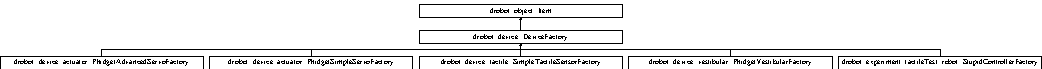
\includegraphics[height=0.930748cm]{classdrobot_1_1device_1_1DeviceFactory}
\end{center}
\end{figure}
\subsection*{Public Member Functions}
\begin{DoxyCompactItemize}
\item 
\hypertarget{classdrobot_1_1device_1_1DeviceFactory_acea73cfabc75353be27326f794cd9f1b}{{\bfseries Device\-Factory} (std\-::string name)}\label{classdrobot_1_1device_1_1DeviceFactory_acea73cfabc75353be27326f794cd9f1b}

\item 
virtual void \hyperlink{classdrobot_1_1device_1_1DeviceFactory_af9234abdb75d5a0129630baabe0c98cc}{create\-From\-Dom\-Element} (Q\-Dom\-Element element, \hyperlink{classdrobot_1_1robot_1_1Robot}{robot\-::\-Robot} $\ast$robot)=0
\begin{DoxyCompactList}\small\item\em create\-From\-Dom\-Element \end{DoxyCompactList}\end{DoxyCompactItemize}
\subsection*{Protected Attributes}
\begin{DoxyCompactItemize}
\item 
\hypertarget{classdrobot_1_1device_1_1DeviceFactory_a4788e52688f9c5bea55fee21015cb25a}{\hyperlink{classdrobot_1_1object_1_1Manager}{object\-::\-Manager}\\*
$<$ \hyperlink{classdrobot_1_1device_1_1channel_1_1ChannelFactory}{channel\-::\-Channel\-Factory} $>$ $\ast$ \hyperlink{classdrobot_1_1device_1_1DeviceFactory_a4788e52688f9c5bea55fee21015cb25a}{\-\_\-channel\-Factories}}\label{classdrobot_1_1device_1_1DeviceFactory_a4788e52688f9c5bea55fee21015cb25a}

\begin{DoxyCompactList}\small\item\em list of this device type's Channel\-Factories. \end{DoxyCompactList}\end{DoxyCompactItemize}


\subsection{Detailed Description}
Base class for Device\-Factories. 

used to create a device from a Dom Tree element (Q\-Dom\-Element) and add it to a robot. The name of the \hyperlink{classdrobot_1_1device_1_1DeviceFactory}{Device\-Factory} must be the same as the tag\-Name of the xml elements. 

\subsection{Member Function Documentation}
\hypertarget{classdrobot_1_1device_1_1DeviceFactory_af9234abdb75d5a0129630baabe0c98cc}{\index{drobot\-::device\-::\-Device\-Factory@{drobot\-::device\-::\-Device\-Factory}!create\-From\-Dom\-Element@{create\-From\-Dom\-Element}}
\index{create\-From\-Dom\-Element@{create\-From\-Dom\-Element}!drobot::device::DeviceFactory@{drobot\-::device\-::\-Device\-Factory}}
\subsubsection[{create\-From\-Dom\-Element}]{\setlength{\rightskip}{0pt plus 5cm}virtual void drobot\-::device\-::\-Device\-Factory\-::create\-From\-Dom\-Element (
\begin{DoxyParamCaption}
\item[{Q\-Dom\-Element}]{element, }
\item[{{\bf robot\-::\-Robot} $\ast$}]{robot}
\end{DoxyParamCaption}
)\hspace{0.3cm}{\ttfamily [pure virtual]}}}\label{classdrobot_1_1device_1_1DeviceFactory_af9234abdb75d5a0129630baabe0c98cc}


create\-From\-Dom\-Element 


\begin{DoxyParams}{Parameters}
{\em element} & \\
\hline
{\em robot} & \\
\hline
\end{DoxyParams}
Creates a device from a Q\-Dom\-Element. This method should add the device of the robots \hyperlink{classdrobot_1_1device_1_1DeviceManager}{Device\-Manager}. If the created \hyperlink{classdrobot_1_1device_1_1Device}{Device} is a Controller the controller property of the robot should also be set. Each device element may contain channel elements which have to be parsed by the channel\-Factories. Also if the device have need of a \hyperlink{classdrobot_1_1device_1_1DeviceBoard}{Device\-Board} it should be added to the \hyperlink{classdrobot_1_1device_1_1DeviceManager}{Device\-Manager} too. See actuator/phidgetadvancedservofactory.\-cpp for an example. 

Implemented in \hyperlink{classdrobot_1_1device_1_1actuator_1_1PhidgetAdvancedServoFactory_a05fc8ede82777f4310ac0cf96e705dbe}{drobot\-::device\-::actuator\-::\-Phidget\-Advanced\-Servo\-Factory}, \hyperlink{classdrobot_1_1device_1_1actuator_1_1PhidgetSimpleServoFactory_a30cab321adc5079711b93fc452028736}{drobot\-::device\-::actuator\-::\-Phidget\-Simple\-Servo\-Factory}, \hyperlink{classdrobot_1_1device_1_1vestibular_1_1PhidgetVestibularFactory_ae877ec4a20bcd09fed94f00952b41f7d}{drobot\-::device\-::vestibular\-::\-Phidget\-Vestibular\-Factory}, \hyperlink{classdrobot_1_1experiment_1_1tactileTest_1_1robot_1_1StupidControllerFactory_aa5d84ac226f532590642a76a74e8df96}{drobot\-::experiment\-::tactile\-Test\-::robot\-::\-Stupid\-Controller\-Factory}, and \hyperlink{classdrobot_1_1device_1_1tactile_1_1SimpleTactileSensorFactory_a727416e619c23b25a01818e33f327d6c}{drobot\-::device\-::tactile\-::\-Simple\-Tactile\-Sensor\-Factory}.



The documentation for this class was generated from the following files\-:\begin{DoxyCompactItemize}
\item 
src/drobot/device/devicefactory.\-h\item 
src/drobot/device/devicefactory.\-cpp\end{DoxyCompactItemize}

\hypertarget{classdrobot_1_1device_1_1DeviceManager}{\section{drobot\-:\-:device\-:\-:Device\-Manager Class Reference}
\label{classdrobot_1_1device_1_1DeviceManager}\index{drobot\-::device\-::\-Device\-Manager@{drobot\-::device\-::\-Device\-Manager}}
}


Special implementation of a Manager for \hyperlink{classdrobot_1_1device_1_1Device}{Device} Items.  




{\ttfamily \#include $<$devicemanager.\-h$>$}

Inheritance diagram for drobot\-:\-:device\-:\-:Device\-Manager\-:\begin{figure}[H]
\begin{center}
\leavevmode
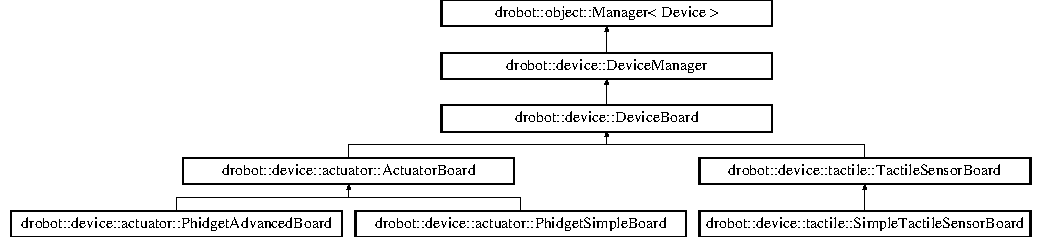
\includegraphics[height=3.185438cm]{classdrobot_1_1device_1_1DeviceManager}
\end{center}
\end{figure}
\subsection*{Public Member Functions}
\begin{DoxyCompactItemize}
\item 
\hypertarget{classdrobot_1_1device_1_1DeviceManager_aba9dc9fb30c827f0ec4bef28da30a831}{{\bfseries Device\-Manager} (std\-::vector$<$ \hyperlink{classdrobot_1_1device_1_1Device}{Device} $\ast$ $>$ items)}\label{classdrobot_1_1device_1_1DeviceManager_aba9dc9fb30c827f0ec4bef28da30a831}

\item 
\hypertarget{classdrobot_1_1device_1_1DeviceManager_a798b2afae1722099f3871e291f825ab7}{virtual void {\bfseries on\-Add} (\hyperlink{classdrobot_1_1device_1_1Device}{Device} $\ast$item)}\label{classdrobot_1_1device_1_1DeviceManager_a798b2afae1722099f3871e291f825ab7}

\item 
\hypertarget{classdrobot_1_1device_1_1DeviceManager_a76832451e5b3bd1809ae6f3af9742c85}{virtual void {\bfseries on\-Remove} (\hyperlink{classdrobot_1_1device_1_1Device}{Device} $\ast$item)}\label{classdrobot_1_1device_1_1DeviceManager_a76832451e5b3bd1809ae6f3af9742c85}

\item 
\hypertarget{classdrobot_1_1device_1_1DeviceManager_a17b122c34ca4c3da6b98d088ea39067e}{void \hyperlink{classdrobot_1_1device_1_1DeviceManager_a17b122c34ca4c3da6b98d088ea39067e}{enable} ()}\label{classdrobot_1_1device_1_1DeviceManager_a17b122c34ca4c3da6b98d088ea39067e}

\begin{DoxyCompactList}\small\item\em enable all devices \end{DoxyCompactList}\item 
\hypertarget{classdrobot_1_1device_1_1DeviceManager_a8680286a13e0f605acf0c23880e5f41d}{void \hyperlink{classdrobot_1_1device_1_1DeviceManager_a8680286a13e0f605acf0c23880e5f41d}{disable} ()}\label{classdrobot_1_1device_1_1DeviceManager_a8680286a13e0f605acf0c23880e5f41d}

\begin{DoxyCompactList}\small\item\em disable all devices \end{DoxyCompactList}\item 
\hypertarget{classdrobot_1_1device_1_1DeviceManager_a2c3e9fba1d847e7a9e0361c4e8c8cd9c}{virtual \hyperlink{classdrobot_1_1device_1_1channel_1_1ChannelManager}{channel\-::\-Channel\-Manager} $\ast$ {\bfseries get\-Channels} ()}\label{classdrobot_1_1device_1_1DeviceManager_a2c3e9fba1d847e7a9e0361c4e8c8cd9c}

\item 
\hypertarget{classdrobot_1_1device_1_1DeviceManager_ab66e717072a3a659031c549093539662}{\hyperlink{classdrobot_1_1object_1_1Manager}{object\-::\-Manager}$<$ \hyperlink{classdrobot_1_1device_1_1DeviceBoard}{Device\-Board} $>$ $\ast$ {\bfseries get\-Device\-Boards} ()}\label{classdrobot_1_1device_1_1DeviceManager_ab66e717072a3a659031c549093539662}

\end{DoxyCompactItemize}
\subsection*{Private Attributes}
\begin{DoxyCompactItemize}
\item 
\hypertarget{classdrobot_1_1device_1_1DeviceManager_ae348bc4e97657d6a2222a61553e4327c}{\hyperlink{classdrobot_1_1device_1_1channel_1_1ChannelManager}{channel\-::\-Channel\-Manager} $\ast$ {\bfseries \-\_\-channels}}\label{classdrobot_1_1device_1_1DeviceManager_ae348bc4e97657d6a2222a61553e4327c}

\item 
\hypertarget{classdrobot_1_1device_1_1DeviceManager_abc4c2b56c5ae9aa5e0a906bc288b87b6}{\hyperlink{classdrobot_1_1object_1_1Manager}{object\-::\-Manager}$<$ \hyperlink{classdrobot_1_1device_1_1DeviceBoard}{Device\-Board} $>$ $\ast$ {\bfseries \-\_\-device\-Boards}}\label{classdrobot_1_1device_1_1DeviceManager_abc4c2b56c5ae9aa5e0a906bc288b87b6}

\end{DoxyCompactItemize}
\subsection*{Additional Inherited Members}


\subsection{Detailed Description}
Special implementation of a Manager for \hyperlink{classdrobot_1_1device_1_1Device}{Device} Items. 

Additionally to the normal Manager implementation it also knows about all the Channels and Device\-Boards of the devices. 

The documentation for this class was generated from the following files\-:\begin{DoxyCompactItemize}
\item 
src/drobot/device/devicemanager.\-h\item 
src/drobot/device/devicemanager.\-cpp\end{DoxyCompactItemize}

\hypertarget{classdrobot_1_1event_1_1Event}{\section{drobot\-:\-:event\-:\-:Event Class Reference}
\label{classdrobot_1_1event_1_1Event}\index{drobot\-::event\-::\-Event@{drobot\-::event\-::\-Event}}
}


The \hyperlink{classdrobot_1_1event_1_1Event}{Event} class.  




{\ttfamily \#include $<$event.\-h$>$}

Inheritance diagram for drobot\-:\-:event\-:\-:Event\-:\begin{figure}[H]
\begin{center}
\leavevmode
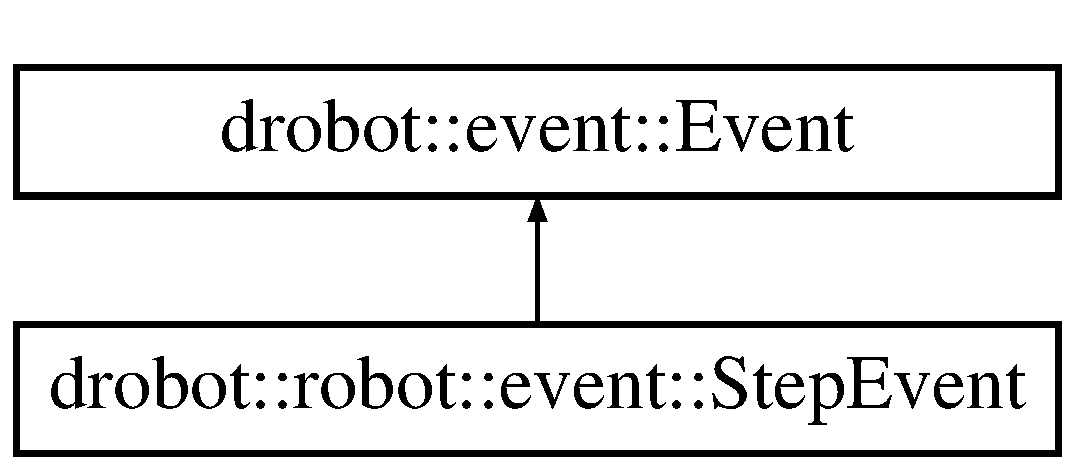
\includegraphics[height=2.000000cm]{classdrobot_1_1event_1_1Event}
\end{center}
\end{figure}
\subsection*{Public Member Functions}
\begin{DoxyCompactItemize}
\item 
\hypertarget{classdrobot_1_1event_1_1Event_af80625172e5af3af44f7e9c760f99969}{{\bfseries Event} (std\-::string type)}\label{classdrobot_1_1event_1_1Event_af80625172e5af3af44f7e9c760f99969}

\item 
std\-::string \hyperlink{classdrobot_1_1event_1_1Event_ab68894db84882d95424818d6bc4b36d4}{get\-Type} ()
\begin{DoxyCompactList}\small\item\em get\-Type. Used to determine which Event\-Listeners to use by the \hyperlink{classdrobot_1_1event_1_1EventManager}{Event\-Manager} class \end{DoxyCompactList}\item 
virtual std\-::string \hyperlink{classdrobot_1_1event_1_1Event_a25b725cbb7dbdb4a41b9c4e9fc3785d8}{to\-String} ()=0
\begin{DoxyCompactList}\small\item\em create a string representatio of this event used for console debugging \end{DoxyCompactList}\end{DoxyCompactItemize}
\subsection*{Private Attributes}
\begin{DoxyCompactItemize}
\item 
\hypertarget{classdrobot_1_1event_1_1Event_a285621fe5004655e8c6924c864d378bd}{std\-::string \hyperlink{classdrobot_1_1event_1_1Event_a285621fe5004655e8c6924c864d378bd}{\-\_\-type}}\label{classdrobot_1_1event_1_1Event_a285621fe5004655e8c6924c864d378bd}

\begin{DoxyCompactList}\small\item\em \-\_\-type of the event. Used to determine which Event\-Listeners to use by the \hyperlink{classdrobot_1_1event_1_1EventManager}{Event\-Manager} class \end{DoxyCompactList}\end{DoxyCompactItemize}


\subsection{Detailed Description}
The \hyperlink{classdrobot_1_1event_1_1Event}{Event} class. 

\subsection{Member Function Documentation}
\hypertarget{classdrobot_1_1event_1_1Event_ab68894db84882d95424818d6bc4b36d4}{\index{drobot\-::event\-::\-Event@{drobot\-::event\-::\-Event}!get\-Type@{get\-Type}}
\index{get\-Type@{get\-Type}!drobot::event::Event@{drobot\-::event\-::\-Event}}
\subsubsection[{get\-Type}]{\setlength{\rightskip}{0pt plus 5cm}std\-::string drobot\-::event\-::\-Event\-::get\-Type (
\begin{DoxyParamCaption}
{}
\end{DoxyParamCaption}
)}}\label{classdrobot_1_1event_1_1Event_ab68894db84882d95424818d6bc4b36d4}


get\-Type. Used to determine which Event\-Listeners to use by the \hyperlink{classdrobot_1_1event_1_1EventManager}{Event\-Manager} class 

\begin{DoxyReturn}{Returns}
the type 
\end{DoxyReturn}
\hypertarget{classdrobot_1_1event_1_1Event_a25b725cbb7dbdb4a41b9c4e9fc3785d8}{\index{drobot\-::event\-::\-Event@{drobot\-::event\-::\-Event}!to\-String@{to\-String}}
\index{to\-String@{to\-String}!drobot::event::Event@{drobot\-::event\-::\-Event}}
\subsubsection[{to\-String}]{\setlength{\rightskip}{0pt plus 5cm}virtual std\-::string drobot\-::event\-::\-Event\-::to\-String (
\begin{DoxyParamCaption}
{}
\end{DoxyParamCaption}
)\hspace{0.3cm}{\ttfamily [pure virtual]}}}\label{classdrobot_1_1event_1_1Event_a25b725cbb7dbdb4a41b9c4e9fc3785d8}


create a string representatio of this event used for console debugging 

\begin{DoxyReturn}{Returns}
the string representation 
\end{DoxyReturn}


Implemented in \hyperlink{classdrobot_1_1robot_1_1event_1_1StepEvent_a40504ba9d43d9db0efdd7a16551af2f3}{drobot\-::robot\-::event\-::\-Step\-Event}.



The documentation for this class was generated from the following files\-:\begin{DoxyCompactItemize}
\item 
src/drobot/event/event.\-h\item 
src/drobot/event/event.\-cpp\end{DoxyCompactItemize}

\hypertarget{classdrobot_1_1event_1_1EventListener}{\section{drobot\-:\-:event\-:\-:Event\-Listener Class Reference}
\label{classdrobot_1_1event_1_1EventListener}\index{drobot\-::event\-::\-Event\-Listener@{drobot\-::event\-::\-Event\-Listener}}
}


Abstract class to be implemented by Event\-Listeners.  




{\ttfamily \#include $<$eventlistener.\-h$>$}

Inheritance diagram for drobot\-:\-:event\-:\-:Event\-Listener\-:\begin{figure}[H]
\begin{center}
\leavevmode
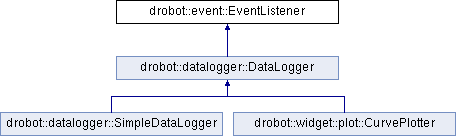
\includegraphics[height=3.000000cm]{classdrobot_1_1event_1_1EventListener}
\end{center}
\end{figure}
\subsection*{Public Member Functions}
\begin{DoxyCompactItemize}
\item 
\hypertarget{classdrobot_1_1event_1_1EventListener_ad9aa9dca8021eaa6d4499f8dca868305}{{\bfseries Event\-Listener} (std\-::string type)}\label{classdrobot_1_1event_1_1EventListener_ad9aa9dca8021eaa6d4499f8dca868305}

\item 
std\-::string \hyperlink{classdrobot_1_1event_1_1EventListener_af6f3b538bc3595de13959d9e35c0449e}{get\-Type} ()
\begin{DoxyCompactList}\small\item\em get\-Type. type of events that are handled by this event\-Listener \end{DoxyCompactList}\item 
virtual void \hyperlink{classdrobot_1_1event_1_1EventListener_ae5e30e4a518f6752a09f44f8dc6cdc51}{on\-Event} (\hyperlink{classdrobot_1_1event_1_1Event}{Event} $\ast$event)=0
\begin{DoxyCompactList}\small\item\em on\-Event. This method is called when an event of this type is fired. \end{DoxyCompactList}\end{DoxyCompactItemize}
\subsection*{Private Attributes}
\begin{DoxyCompactItemize}
\item 
\hypertarget{classdrobot_1_1event_1_1EventListener_aeb0390f315d94929c93797d858d0fb6e}{std\-::string \hyperlink{classdrobot_1_1event_1_1EventListener_aeb0390f315d94929c93797d858d0fb6e}{\-\_\-type}}\label{classdrobot_1_1event_1_1EventListener_aeb0390f315d94929c93797d858d0fb6e}

\begin{DoxyCompactList}\small\item\em type of events that are handled by this event\-Listener \end{DoxyCompactList}\end{DoxyCompactItemize}


\subsection{Detailed Description}
Abstract class to be implemented by Event\-Listeners. 

\subsection{Member Function Documentation}
\hypertarget{classdrobot_1_1event_1_1EventListener_af6f3b538bc3595de13959d9e35c0449e}{\index{drobot\-::event\-::\-Event\-Listener@{drobot\-::event\-::\-Event\-Listener}!get\-Type@{get\-Type}}
\index{get\-Type@{get\-Type}!drobot::event::EventListener@{drobot\-::event\-::\-Event\-Listener}}
\subsubsection[{get\-Type}]{\setlength{\rightskip}{0pt plus 5cm}std\-::string drobot\-::event\-::\-Event\-Listener\-::get\-Type (
\begin{DoxyParamCaption}
{}
\end{DoxyParamCaption}
)}}\label{classdrobot_1_1event_1_1EventListener_af6f3b538bc3595de13959d9e35c0449e}


get\-Type. type of events that are handled by this event\-Listener 

\begin{DoxyReturn}{Returns}
the event type 
\end{DoxyReturn}
\hypertarget{classdrobot_1_1event_1_1EventListener_ae5e30e4a518f6752a09f44f8dc6cdc51}{\index{drobot\-::event\-::\-Event\-Listener@{drobot\-::event\-::\-Event\-Listener}!on\-Event@{on\-Event}}
\index{on\-Event@{on\-Event}!drobot::event::EventListener@{drobot\-::event\-::\-Event\-Listener}}
\subsubsection[{on\-Event}]{\setlength{\rightskip}{0pt plus 5cm}virtual void drobot\-::event\-::\-Event\-Listener\-::on\-Event (
\begin{DoxyParamCaption}
\item[{{\bf Event} $\ast$}]{event}
\end{DoxyParamCaption}
)\hspace{0.3cm}{\ttfamily [pure virtual]}}}\label{classdrobot_1_1event_1_1EventListener_ae5e30e4a518f6752a09f44f8dc6cdc51}


on\-Event. This method is called when an event of this type is fired. 


\begin{DoxyParams}{Parameters}
{\em event} & fired \\
\hline
\end{DoxyParams}


Implemented in \hyperlink{classdrobot_1_1datalogger_1_1DataLogger_a830fcb8f0b8b261bba22cfce46f4d309}{drobot\-::datalogger\-::\-Data\-Logger}.



The documentation for this class was generated from the following files\-:\begin{DoxyCompactItemize}
\item 
/home/imanol/workspace/drobot/new/src/drobot/event/eventlistener.\-h\item 
/home/imanol/workspace/drobot/new/src/drobot/event/eventlistener.\-cpp\end{DoxyCompactItemize}

\hypertarget{classdrobot_1_1event_1_1EventManager}{\section{drobot\-:\-:event\-:\-:Event\-Manager Class Reference}
\label{classdrobot_1_1event_1_1EventManager}\index{drobot\-::event\-::\-Event\-Manager@{drobot\-::event\-::\-Event\-Manager}}
}


Used for managing events.  




{\ttfamily \#include $<$eventmanager.\-h$>$}

\subsection*{Public Member Functions}
\begin{DoxyCompactItemize}
\item 
void \hyperlink{classdrobot_1_1event_1_1EventManager_a9d8046d9f53a50414294385a2cf3b73f}{register\-Event\-Listener} (\hyperlink{classdrobot_1_1event_1_1EventListener}{Event\-Listener} $\ast$event\-Listener)
\begin{DoxyCompactList}\small\item\em add an \hyperlink{classdrobot_1_1event_1_1EventListener}{Event\-Listener} \end{DoxyCompactList}\item 
void \hyperlink{classdrobot_1_1event_1_1EventManager_a947d28a494697d51eb33e4da4878f4e6}{unregister\-Event\-Listener} (\hyperlink{classdrobot_1_1event_1_1EventListener}{Event\-Listener} $\ast$event\-Listener)
\begin{DoxyCompactList}\small\item\em remove an \hyperlink{classdrobot_1_1event_1_1EventListener}{Event\-Listener} \end{DoxyCompactList}\item 
void \hyperlink{classdrobot_1_1event_1_1EventManager_a8961eb4b97c48e0e02566b4ccffca98a}{fire\-Event} (\hyperlink{classdrobot_1_1event_1_1Event}{Event} $\ast$event)
\begin{DoxyCompactList}\small\item\em fire \hyperlink{classdrobot_1_1event_1_1Event}{Event} \end{DoxyCompactList}\end{DoxyCompactItemize}
\subsection*{Private Attributes}
\begin{DoxyCompactItemize}
\item 
\hypertarget{classdrobot_1_1event_1_1EventManager_a798786a397eacf61b7ee79a6c5238605}{std\-::map$<$ std\-::string, \\*
std\-::vector$<$ \hyperlink{classdrobot_1_1event_1_1EventListener}{Event\-Listener} $\ast$ $>$ $>$ {\bfseries \-\_\-event\-Listeners}}\label{classdrobot_1_1event_1_1EventManager_a798786a397eacf61b7ee79a6c5238605}

\end{DoxyCompactItemize}


\subsection{Detailed Description}
Used for managing events. 

Each robot has it's own \hyperlink{classdrobot_1_1event_1_1EventManager}{Event\-Manager}. 

\subsection{Member Function Documentation}
\hypertarget{classdrobot_1_1event_1_1EventManager_a8961eb4b97c48e0e02566b4ccffca98a}{\index{drobot\-::event\-::\-Event\-Manager@{drobot\-::event\-::\-Event\-Manager}!fire\-Event@{fire\-Event}}
\index{fire\-Event@{fire\-Event}!drobot::event::EventManager@{drobot\-::event\-::\-Event\-Manager}}
\subsubsection[{fire\-Event}]{\setlength{\rightskip}{0pt plus 5cm}void drobot\-::event\-::\-Event\-Manager\-::fire\-Event (
\begin{DoxyParamCaption}
\item[{{\bf Event} $\ast$}]{event}
\end{DoxyParamCaption}
)}}\label{classdrobot_1_1event_1_1EventManager_a8961eb4b97c48e0e02566b4ccffca98a}


fire \hyperlink{classdrobot_1_1event_1_1Event}{Event} 


\begin{DoxyParams}{Parameters}
{\em event} & \\
\hline
\end{DoxyParams}
\hypertarget{classdrobot_1_1event_1_1EventManager_a9d8046d9f53a50414294385a2cf3b73f}{\index{drobot\-::event\-::\-Event\-Manager@{drobot\-::event\-::\-Event\-Manager}!register\-Event\-Listener@{register\-Event\-Listener}}
\index{register\-Event\-Listener@{register\-Event\-Listener}!drobot::event::EventManager@{drobot\-::event\-::\-Event\-Manager}}
\subsubsection[{register\-Event\-Listener}]{\setlength{\rightskip}{0pt plus 5cm}void drobot\-::event\-::\-Event\-Manager\-::register\-Event\-Listener (
\begin{DoxyParamCaption}
\item[{{\bf Event\-Listener} $\ast$}]{event\-Listener}
\end{DoxyParamCaption}
)}}\label{classdrobot_1_1event_1_1EventManager_a9d8046d9f53a50414294385a2cf3b73f}


add an \hyperlink{classdrobot_1_1event_1_1EventListener}{Event\-Listener} 


\begin{DoxyParams}{Parameters}
{\em event\-Listener} & \\
\hline
\end{DoxyParams}
\hypertarget{classdrobot_1_1event_1_1EventManager_a947d28a494697d51eb33e4da4878f4e6}{\index{drobot\-::event\-::\-Event\-Manager@{drobot\-::event\-::\-Event\-Manager}!unregister\-Event\-Listener@{unregister\-Event\-Listener}}
\index{unregister\-Event\-Listener@{unregister\-Event\-Listener}!drobot::event::EventManager@{drobot\-::event\-::\-Event\-Manager}}
\subsubsection[{unregister\-Event\-Listener}]{\setlength{\rightskip}{0pt plus 5cm}void drobot\-::event\-::\-Event\-Manager\-::unregister\-Event\-Listener (
\begin{DoxyParamCaption}
\item[{{\bf Event\-Listener} $\ast$}]{event\-Listener}
\end{DoxyParamCaption}
)}}\label{classdrobot_1_1event_1_1EventManager_a947d28a494697d51eb33e4da4878f4e6}


remove an \hyperlink{classdrobot_1_1event_1_1EventListener}{Event\-Listener} 


\begin{DoxyParams}{Parameters}
{\em event\-Listener} & \\
\hline
\end{DoxyParams}


The documentation for this class was generated from the following files\-:\begin{DoxyCompactItemize}
\item 
src/drobot/event/eventmanager.\-h\item 
src/drobot/event/eventmanager.\-cpp\end{DoxyCompactItemize}

\hypertarget{classdrobot_1_1util_1_1Exception}{\section{drobot\-:\-:util\-:\-:Exception Class Reference}
\label{classdrobot_1_1util_1_1Exception}\index{drobot\-::util\-::\-Exception@{drobot\-::util\-::\-Exception}}
}


The \hyperlink{classdrobot_1_1util_1_1Exception}{Exception} class is the base class for all exceptions.  




{\ttfamily \#include $<$exception.\-h$>$}

\subsection*{Public Member Functions}
\begin{DoxyCompactItemize}
\item 
\hypertarget{classdrobot_1_1util_1_1Exception_a6a910e1c09a10ce2bad7fabec0b08443}{{\bfseries Exception} (std\-::string message)}\label{classdrobot_1_1util_1_1Exception_a6a910e1c09a10ce2bad7fabec0b08443}

\item 
\hypertarget{classdrobot_1_1util_1_1Exception_a335a60268148f7389c21a12fe48bafcf}{std\-::string {\bfseries get\-Message} ()}\label{classdrobot_1_1util_1_1Exception_a335a60268148f7389c21a12fe48bafcf}

\item 
\hyperlink{classdrobot_1_1util_1_1Exception}{Exception} \& \hyperlink{classdrobot_1_1util_1_1Exception_a551cef708ba29da1d9129ec464e99a75}{operator$<$$<$} (std\-::string message)
\begin{DoxyCompactList}\small\item\em operator $<$$<$ is used to append a string to the message \end{DoxyCompactList}\item 
\hyperlink{classdrobot_1_1util_1_1Exception}{Exception} \& \hyperlink{classdrobot_1_1util_1_1Exception_a1e79ba068991f137adc7cdccf1b0f054}{operator$<$$<$} (int message)
\begin{DoxyCompactList}\small\item\em operator $<$$<$ is used to append a int to the message \end{DoxyCompactList}\item 
\hyperlink{classdrobot_1_1util_1_1Exception}{Exception} \& \hyperlink{classdrobot_1_1util_1_1Exception_aa817875aaf71163089f3e13e2e0732e6}{operator$<$$<$} (double message)
\begin{DoxyCompactList}\small\item\em operator $<$$<$ is used to append a double to the message \end{DoxyCompactList}\end{DoxyCompactItemize}
\subsection*{Private Attributes}
\begin{DoxyCompactItemize}
\item 
\hypertarget{classdrobot_1_1util_1_1Exception_abbccadd97e9a688cd47c170c4e361c1b}{std\-::string {\bfseries \-\_\-message}}\label{classdrobot_1_1util_1_1Exception_abbccadd97e9a688cd47c170c4e361c1b}

\end{DoxyCompactItemize}


\subsection{Detailed Description}
The \hyperlink{classdrobot_1_1util_1_1Exception}{Exception} class is the base class for all exceptions. 

\subsection{Member Function Documentation}
\hypertarget{classdrobot_1_1util_1_1Exception_a551cef708ba29da1d9129ec464e99a75}{\index{drobot\-::util\-::\-Exception@{drobot\-::util\-::\-Exception}!operator$<$$<$@{operator$<$$<$}}
\index{operator$<$$<$@{operator$<$$<$}!drobot::util::Exception@{drobot\-::util\-::\-Exception}}
\subsubsection[{operator$<$$<$}]{\setlength{\rightskip}{0pt plus 5cm}{\bf Exception} \& drobot\-::util\-::\-Exception\-::operator$<$$<$ (
\begin{DoxyParamCaption}
\item[{std\-::string}]{message}
\end{DoxyParamCaption}
)}}\label{classdrobot_1_1util_1_1Exception_a551cef708ba29da1d9129ec464e99a75}


operator $<$$<$ is used to append a string to the message 


\begin{DoxyParams}{Parameters}
{\em message} & \\
\hline
\end{DoxyParams}
\begin{DoxyReturn}{Returns}
reference to the exception 
\end{DoxyReturn}
\hypertarget{classdrobot_1_1util_1_1Exception_a1e79ba068991f137adc7cdccf1b0f054}{\index{drobot\-::util\-::\-Exception@{drobot\-::util\-::\-Exception}!operator$<$$<$@{operator$<$$<$}}
\index{operator$<$$<$@{operator$<$$<$}!drobot::util::Exception@{drobot\-::util\-::\-Exception}}
\subsubsection[{operator$<$$<$}]{\setlength{\rightskip}{0pt plus 5cm}{\bf Exception} \& drobot\-::util\-::\-Exception\-::operator$<$$<$ (
\begin{DoxyParamCaption}
\item[{int}]{message}
\end{DoxyParamCaption}
)}}\label{classdrobot_1_1util_1_1Exception_a1e79ba068991f137adc7cdccf1b0f054}


operator $<$$<$ is used to append a int to the message 


\begin{DoxyParams}{Parameters}
{\em message} & \\
\hline
\end{DoxyParams}
\begin{DoxyReturn}{Returns}
reference to the exception 
\end{DoxyReturn}
\hypertarget{classdrobot_1_1util_1_1Exception_aa817875aaf71163089f3e13e2e0732e6}{\index{drobot\-::util\-::\-Exception@{drobot\-::util\-::\-Exception}!operator$<$$<$@{operator$<$$<$}}
\index{operator$<$$<$@{operator$<$$<$}!drobot::util::Exception@{drobot\-::util\-::\-Exception}}
\subsubsection[{operator$<$$<$}]{\setlength{\rightskip}{0pt plus 5cm}{\bf Exception} \& drobot\-::util\-::\-Exception\-::operator$<$$<$ (
\begin{DoxyParamCaption}
\item[{double}]{message}
\end{DoxyParamCaption}
)}}\label{classdrobot_1_1util_1_1Exception_aa817875aaf71163089f3e13e2e0732e6}


operator $<$$<$ is used to append a double to the message 


\begin{DoxyParams}{Parameters}
{\em message} & \\
\hline
\end{DoxyParams}
\begin{DoxyReturn}{Returns}
reference to the exception 
\end{DoxyReturn}


The documentation for this class was generated from the following files\-:\begin{DoxyCompactItemize}
\item 
src/drobot/util/exception.\-h\item 
src/drobot/util/exception.\-cpp\end{DoxyCompactItemize}

\hypertarget{classdrobot_1_1object_1_1Item}{\section{drobot\-:\-:object\-:\-:Item Class Reference}
\label{classdrobot_1_1object_1_1Item}\index{drobot\-::object\-::\-Item@{drobot\-::object\-::\-Item}}
}


Base class for most of the classes. Can be added to a \hyperlink{classdrobot_1_1object_1_1Manager}{Manager} to prevent memory leaks.  




{\ttfamily \#include $<$item.\-h$>$}

Inheritance diagram for drobot\-:\-:object\-:\-:Item\-:\begin{figure}[H]
\begin{center}
\leavevmode
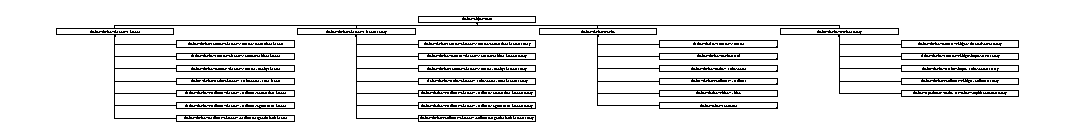
\includegraphics[height=1.412556cm]{classdrobot_1_1object_1_1Item}
\end{center}
\end{figure}
\subsection*{Public Member Functions}
\begin{DoxyCompactItemize}
\item 
\hypertarget{classdrobot_1_1object_1_1Item_acc8d4d20dfcbb135b14eea75f823bffa}{{\bfseries Item} (std\-::string name)}\label{classdrobot_1_1object_1_1Item_acc8d4d20dfcbb135b14eea75f823bffa}

\item 
\hypertarget{classdrobot_1_1object_1_1Item_afe4a17af245f08bbe5b34ff0902bd7e5}{void {\bfseries set\-Name} (std\-::string name)}\label{classdrobot_1_1object_1_1Item_afe4a17af245f08bbe5b34ff0902bd7e5}

\item 
\hypertarget{classdrobot_1_1object_1_1Item_a24d83fed092adae39ea5947454e03b2f}{virtual std\-::string {\bfseries get\-Name} ()}\label{classdrobot_1_1object_1_1Item_a24d83fed092adae39ea5947454e03b2f}

\end{DoxyCompactItemize}
\subsection*{Protected Attributes}
\begin{DoxyCompactItemize}
\item 
\hypertarget{classdrobot_1_1object_1_1Item_a319f13abefdd8e4abb5da064a7227bb2}{std\-::string \hyperlink{classdrobot_1_1object_1_1Item_a319f13abefdd8e4abb5da064a7227bb2}{\-\_\-name}}\label{classdrobot_1_1object_1_1Item_a319f13abefdd8e4abb5da064a7227bb2}

\begin{DoxyCompactList}\small\item\em name of the item \end{DoxyCompactList}\end{DoxyCompactItemize}


\subsection{Detailed Description}
Base class for most of the classes. Can be added to a \hyperlink{classdrobot_1_1object_1_1Manager}{Manager} to prevent memory leaks. 

The documentation for this class was generated from the following files\-:\begin{DoxyCompactItemize}
\item 
/home/imanol/workspace/drobot/new/src/drobot/object/item.\-h\item 
/home/imanol/workspace/drobot/new/src/drobot/object/item.\-cpp\end{DoxyCompactItemize}

\hypertarget{classdrobot_1_1device_1_1channel_1_1LinearNormalizer}{\section{drobot\-:\-:device\-:\-:channel\-:\-:Linear\-Normalizer Class Reference}
\label{classdrobot_1_1device_1_1channel_1_1LinearNormalizer}\index{drobot\-::device\-::channel\-::\-Linear\-Normalizer@{drobot\-::device\-::channel\-::\-Linear\-Normalizer}}
}


The \hyperlink{classdrobot_1_1device_1_1channel_1_1LinearNormalizer}{Linear\-Normalizer} class.  




{\ttfamily \#include $<$linearnormalizer.\-h$>$}

Inheritance diagram for drobot\-:\-:device\-:\-:channel\-:\-:Linear\-Normalizer\-:\begin{figure}[H]
\begin{center}
\leavevmode
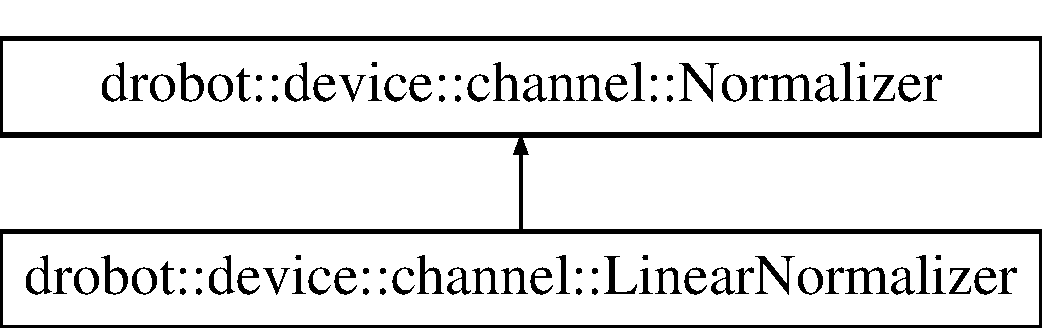
\includegraphics[height=2.000000cm]{classdrobot_1_1device_1_1channel_1_1LinearNormalizer}
\end{center}
\end{figure}
\subsection*{Public Member Functions}
\begin{DoxyCompactItemize}
\item 
\hypertarget{classdrobot_1_1device_1_1channel_1_1LinearNormalizer_a84fec2614263c8bf35ce13fad7b2fc9e}{{\bfseries Linear\-Normalizer} (double min, double max)}\label{classdrobot_1_1device_1_1channel_1_1LinearNormalizer_a84fec2614263c8bf35ce13fad7b2fc9e}

\item 
virtual double \hyperlink{classdrobot_1_1device_1_1channel_1_1LinearNormalizer_a56e9bacaecd6b5310525d60ecd1a0f5c}{normalize} (double value)
\begin{DoxyCompactList}\small\item\em normalize value to the interval from 0 to 1 \end{DoxyCompactList}\item 
virtual double \hyperlink{classdrobot_1_1device_1_1channel_1_1LinearNormalizer_a7db474fa6bcb13adb6ffa2044d512b6d}{denormalize} (double value)
\begin{DoxyCompactList}\small\item\em denormalize value from an interval from 0 to 1 to it's original range \end{DoxyCompactList}\end{DoxyCompactItemize}
\subsection*{Private Attributes}
\begin{DoxyCompactItemize}
\item 
\hypertarget{classdrobot_1_1device_1_1channel_1_1LinearNormalizer_a4e40a22b62c17cac222bb4daa0acf121}{double {\bfseries \-\_\-min}}\label{classdrobot_1_1device_1_1channel_1_1LinearNormalizer_a4e40a22b62c17cac222bb4daa0acf121}

\item 
\hypertarget{classdrobot_1_1device_1_1channel_1_1LinearNormalizer_a78515684623f4596d0af189bac9ac4b4}{double {\bfseries \-\_\-max}}\label{classdrobot_1_1device_1_1channel_1_1LinearNormalizer_a78515684623f4596d0af189bac9ac4b4}

\end{DoxyCompactItemize}


\subsection{Detailed Description}
The \hyperlink{classdrobot_1_1device_1_1channel_1_1LinearNormalizer}{Linear\-Normalizer} class. 

linearly normalizes values from \-\_\-min to \-\_\-max to a 0 to 1 interval 

\subsection{Member Function Documentation}
\hypertarget{classdrobot_1_1device_1_1channel_1_1LinearNormalizer_a7db474fa6bcb13adb6ffa2044d512b6d}{\index{drobot\-::device\-::channel\-::\-Linear\-Normalizer@{drobot\-::device\-::channel\-::\-Linear\-Normalizer}!denormalize@{denormalize}}
\index{denormalize@{denormalize}!drobot::device::channel::LinearNormalizer@{drobot\-::device\-::channel\-::\-Linear\-Normalizer}}
\subsubsection[{denormalize}]{\setlength{\rightskip}{0pt plus 5cm}double drobot\-::device\-::channel\-::\-Linear\-Normalizer\-::denormalize (
\begin{DoxyParamCaption}
\item[{double}]{value}
\end{DoxyParamCaption}
)\hspace{0.3cm}{\ttfamily [virtual]}}}\label{classdrobot_1_1device_1_1channel_1_1LinearNormalizer_a7db474fa6bcb13adb6ffa2044d512b6d}


denormalize value from an interval from 0 to 1 to it's original range 


\begin{DoxyParams}{Parameters}
{\em value} & \\
\hline
\end{DoxyParams}
\begin{DoxyReturn}{Returns}
denormalized value 
\end{DoxyReturn}


Implements \hyperlink{classdrobot_1_1device_1_1channel_1_1Normalizer_ab95ae6d2d813c70bd99efb998b78d163}{drobot\-::device\-::channel\-::\-Normalizer}.

\hypertarget{classdrobot_1_1device_1_1channel_1_1LinearNormalizer_a56e9bacaecd6b5310525d60ecd1a0f5c}{\index{drobot\-::device\-::channel\-::\-Linear\-Normalizer@{drobot\-::device\-::channel\-::\-Linear\-Normalizer}!normalize@{normalize}}
\index{normalize@{normalize}!drobot::device::channel::LinearNormalizer@{drobot\-::device\-::channel\-::\-Linear\-Normalizer}}
\subsubsection[{normalize}]{\setlength{\rightskip}{0pt plus 5cm}double drobot\-::device\-::channel\-::\-Linear\-Normalizer\-::normalize (
\begin{DoxyParamCaption}
\item[{double}]{value}
\end{DoxyParamCaption}
)\hspace{0.3cm}{\ttfamily [virtual]}}}\label{classdrobot_1_1device_1_1channel_1_1LinearNormalizer_a56e9bacaecd6b5310525d60ecd1a0f5c}


normalize value to the interval from 0 to 1 


\begin{DoxyParams}{Parameters}
{\em value} & \\
\hline
\end{DoxyParams}
\begin{DoxyReturn}{Returns}
normalized value 
\end{DoxyReturn}


Implements \hyperlink{classdrobot_1_1device_1_1channel_1_1Normalizer_a815d0fa0ae0f301137b7a79baff020f2}{drobot\-::device\-::channel\-::\-Normalizer}.



The documentation for this class was generated from the following files\-:\begin{DoxyCompactItemize}
\item 
/home/imanol/workspace/drobot/new/src/drobot/device/channel/linearnormalizer.\-h\item 
/home/imanol/workspace/drobot/new/src/drobot/device/channel/linearnormalizer.\-cpp\end{DoxyCompactItemize}

\hypertarget{classdrobot_1_1experiment_1_1tactileTest_1_1widget_1_1MainWidget}{\section{drobot\-:\-:experiment\-:\-:tactile\-Test\-:\-:widget\-:\-:Main\-Widget Class Reference}
\label{classdrobot_1_1experiment_1_1tactileTest_1_1widget_1_1MainWidget}\index{drobot\-::experiment\-::tactile\-Test\-::widget\-::\-Main\-Widget@{drobot\-::experiment\-::tactile\-Test\-::widget\-::\-Main\-Widget}}
}
Inheritance diagram for drobot\-:\-:experiment\-:\-:tactile\-Test\-:\-:widget\-:\-:Main\-Widget\-:\begin{figure}[H]
\begin{center}
\leavevmode
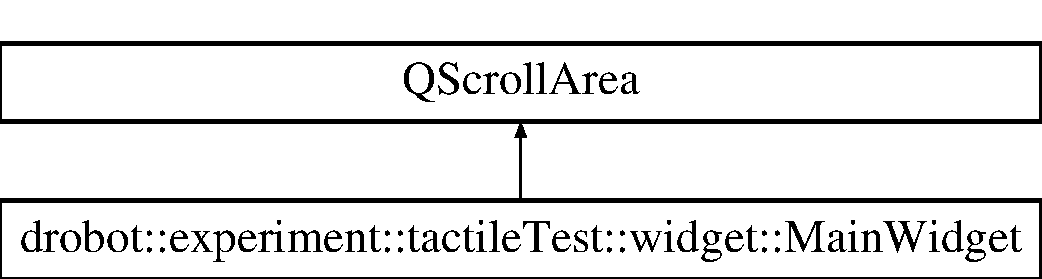
\includegraphics[height=2.000000cm]{classdrobot_1_1experiment_1_1tactileTest_1_1widget_1_1MainWidget}
\end{center}
\end{figure}
\subsection*{Public Member Functions}
\begin{DoxyCompactItemize}
\item 
\hypertarget{classdrobot_1_1experiment_1_1tactileTest_1_1widget_1_1MainWidget_a65b43165ab8b3ce3b6a38f62f27a1c8b}{{\bfseries Main\-Widget} (Q\-Widget $\ast$parent=0)}\label{classdrobot_1_1experiment_1_1tactileTest_1_1widget_1_1MainWidget_a65b43165ab8b3ce3b6a38f62f27a1c8b}

\end{DoxyCompactItemize}
\subsection*{Private Attributes}
\begin{DoxyCompactItemize}
\item 
\hypertarget{classdrobot_1_1experiment_1_1tactileTest_1_1widget_1_1MainWidget_a2a6ebbf269a8bae0f9a5aef294d3d7c6}{Ui\-::\-Main\-Widget $\ast$ {\bfseries ui}}\label{classdrobot_1_1experiment_1_1tactileTest_1_1widget_1_1MainWidget_a2a6ebbf269a8bae0f9a5aef294d3d7c6}

\end{DoxyCompactItemize}


The documentation for this class was generated from the following files\-:\begin{DoxyCompactItemize}
\item 
/home/imanol/workspace/drobot/new/src/drobot/experiment/tactile\-Test/widget/tactiletestmainwidget.\-h\item 
/home/imanol/workspace/drobot/new/src/drobot/experiment/tactile\-Test/widget/tactiletestmainwidget.\-cpp\end{DoxyCompactItemize}

\hypertarget{classdrobot_1_1widget_1_1MainWindow}{\section{drobot\-:\-:widget\-:\-:Main\-Window Class Reference}
\label{classdrobot_1_1widget_1_1MainWindow}\index{drobot\-::widget\-::\-Main\-Window@{drobot\-::widget\-::\-Main\-Window}}
}
Inheritance diagram for drobot\-:\-:widget\-:\-:Main\-Window\-:\begin{figure}[H]
\begin{center}
\leavevmode
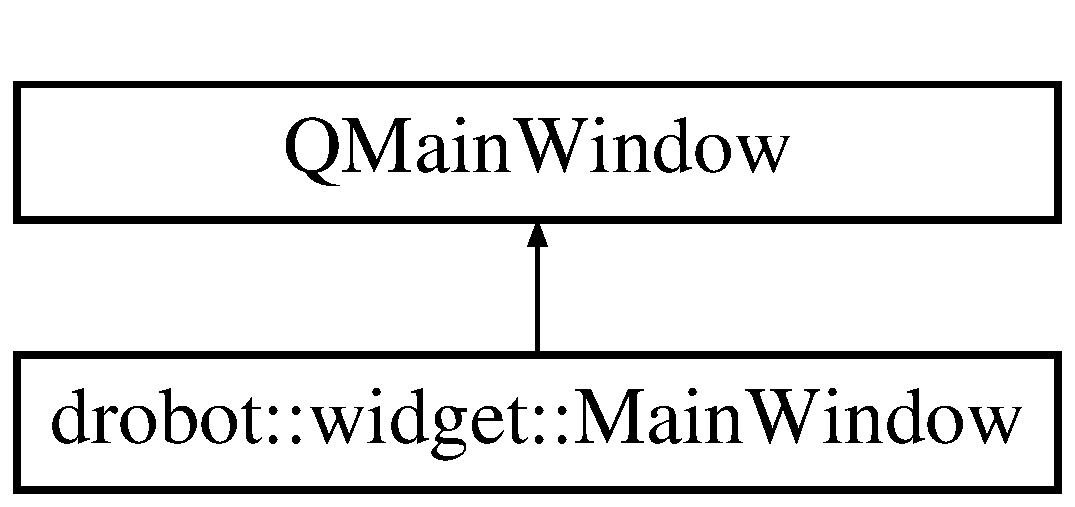
\includegraphics[height=2.000000cm]{classdrobot_1_1widget_1_1MainWindow}
\end{center}
\end{figure}
\subsection*{Public Slots}
\begin{DoxyCompactItemize}
\item 
\hypertarget{classdrobot_1_1widget_1_1MainWindow_a92780b8f96de5ace56e84ee1e3ef70a2}{void {\bfseries on\-Program\-Launch} ()}\label{classdrobot_1_1widget_1_1MainWindow_a92780b8f96de5ace56e84ee1e3ef70a2}

\end{DoxyCompactItemize}
\subsection*{Public Member Functions}
\begin{DoxyCompactItemize}
\item 
\hypertarget{classdrobot_1_1widget_1_1MainWindow_a3bc62fbbc0ba5600e8c757fde568a2cb}{{\bfseries Main\-Window} (Q\-Widget $\ast$parent=0)}\label{classdrobot_1_1widget_1_1MainWindow_a3bc62fbbc0ba5600e8c757fde568a2cb}

\end{DoxyCompactItemize}
\subsection*{Private Attributes}
\begin{DoxyCompactItemize}
\item 
\hypertarget{classdrobot_1_1widget_1_1MainWindow_ac4f80ce65cb4cb0f464b13fe9757503a}{Ui\-::\-Main\-Window $\ast$ {\bfseries ui}}\label{classdrobot_1_1widget_1_1MainWindow_ac4f80ce65cb4cb0f464b13fe9757503a}

\item 
\hypertarget{classdrobot_1_1widget_1_1MainWindow_a98317c5c39848f3dea6696d3c6f29de3}{\hyperlink{classdrobot_1_1program_1_1ProgramManager}{drobot\-::program\-::\-Program\-Manager} $\ast$ {\bfseries \-\_\-program\-Manager}}\label{classdrobot_1_1widget_1_1MainWindow_a98317c5c39848f3dea6696d3c6f29de3}

\end{DoxyCompactItemize}


The documentation for this class was generated from the following files\-:\begin{DoxyCompactItemize}
\item 
src/drobot/widget/mainwindow.\-h\item 
src/drobot/widget/mainwindow.\-cpp\end{DoxyCompactItemize}

\hypertarget{classdrobot_1_1object_1_1Manager}{\section{drobot\-:\-:object\-:\-:Manager$<$ T $>$ Class Template Reference}
\label{classdrobot_1_1object_1_1Manager}\index{drobot\-::object\-::\-Manager$<$ T $>$@{drobot\-::object\-::\-Manager$<$ T $>$}}
}


\hyperlink{classdrobot_1_1object_1_1Item}{Item} container, can be used to prevent memory leaks.  




{\ttfamily \#include $<$manager.\-h$>$}

\subsection*{Public Member Functions}
\begin{DoxyCompactItemize}
\item 
\hypertarget{classdrobot_1_1object_1_1Manager_a383ef791e44bd1349e078ed183094e5f}{{\bfseries Manager} (std\-::vector$<$ T $\ast$ $>$ items)}\label{classdrobot_1_1object_1_1Manager_a383ef791e44bd1349e078ed183094e5f}

\item 
std\-::vector$<$ T $\ast$ $>$ \hyperlink{classdrobot_1_1object_1_1Manager_a4a9b34e5b7f42b6acafc99bde8d02e61}{values} () const 
\item 
std\-::vector$<$ std\-::string $>$ \hyperlink{classdrobot_1_1object_1_1Manager_a50065ba053bb7e4ebbb0982b2c41abc7}{keys} () const 
\item 
T $\ast$ \hyperlink{classdrobot_1_1object_1_1Manager_a5e04e5974661624d8700b9013dc35246}{get} (std\-::string name)
\item 
bool \hyperlink{classdrobot_1_1object_1_1Manager_a2ef8b37b97245a3b525f0f7cc8a68049}{add} (T $\ast$item)
\begin{DoxyCompactList}\small\item\em adds an item \end{DoxyCompactList}\item 
void \hyperlink{classdrobot_1_1object_1_1Manager_af14a346a13fa1948e97c35458d5f3047}{add} (std\-::vector$<$ T $\ast$ $>$ items)
\begin{DoxyCompactList}\small\item\em adds a list of items \end{DoxyCompactList}\item 
virtual void \hyperlink{classdrobot_1_1object_1_1Manager_ae1a7f38749f66bc4be0e0e0350a5ae68}{on\-Add} (T $\ast$item)
\begin{DoxyCompactList}\small\item\em called when an item is added \end{DoxyCompactList}\item 
T $\ast$ \hyperlink{classdrobot_1_1object_1_1Manager_ad2023f514760d5ae1a4c72f00724e4e9}{remove} (std\-::string name)
\begin{DoxyCompactList}\small\item\em removes an item by its name \end{DoxyCompactList}\item 
T $\ast$ \hyperlink{classdrobot_1_1object_1_1Manager_a1e60717d659da8a4b83d9b6397f0926e}{remove} (T $\ast$item)
\begin{DoxyCompactList}\small\item\em removes an item \end{DoxyCompactList}\item 
virtual void \hyperlink{classdrobot_1_1object_1_1Manager_a17b34bb3d364509c925a7dade1fef14b}{on\-Remove} (T $\ast$item)
\begin{DoxyCompactList}\small\item\em called when an item is removed \end{DoxyCompactList}\item 
std\-::vector$<$ T $\ast$ $>$ \hyperlink{classdrobot_1_1object_1_1Manager_a47e24b1186210a6232f8da62551902fb}{remove} (std\-::vector$<$ T $\ast$ $>$ items)
\begin{DoxyCompactList}\small\item\em removes a list of items \end{DoxyCompactList}\item 
bool \hyperlink{classdrobot_1_1object_1_1Manager_a4bde99ebbba5be83e3d6144c75335bf5}{has} (std\-::string name)
\begin{DoxyCompactList}\small\item\em checks if item is in the list by its name \end{DoxyCompactList}\item 
bool \hyperlink{classdrobot_1_1object_1_1Manager_ae7d90ba11895c86b957ac4b81851a0d7}{has} (T $\ast$item)
\begin{DoxyCompactList}\small\item\em checks if item is in the list \end{DoxyCompactList}\item 
\hypertarget{classdrobot_1_1object_1_1Manager_ae40cda4743e17cc7736b24db57e53268}{void \hyperlink{classdrobot_1_1object_1_1Manager_ae40cda4743e17cc7736b24db57e53268}{clear} ()}\label{classdrobot_1_1object_1_1Manager_ae40cda4743e17cc7736b24db57e53268}

\begin{DoxyCompactList}\small\item\em removes all the items \end{DoxyCompactList}\end{DoxyCompactItemize}
\subsection*{Protected Attributes}
\begin{DoxyCompactItemize}
\item 
\hypertarget{classdrobot_1_1object_1_1Manager_af54347142e8014f7faa02acb14f7ace3}{bool \hyperlink{classdrobot_1_1object_1_1Manager_af54347142e8014f7faa02acb14f7ace3}{\-\_\-delete\-Items\-On\-Destroy}}\label{classdrobot_1_1object_1_1Manager_af54347142e8014f7faa02acb14f7ace3}

\begin{DoxyCompactList}\small\item\em flag indicating wether the items should be deleted in the Destructor. \end{DoxyCompactList}\end{DoxyCompactItemize}
\subsection*{Private Attributes}
\begin{DoxyCompactItemize}
\item 
\hypertarget{classdrobot_1_1object_1_1Manager_a6c91eabd63264c09225f5c35cd0cd792}{std\-::map$<$ std\-::string, T $\ast$ $>$ \hyperlink{classdrobot_1_1object_1_1Manager_a6c91eabd63264c09225f5c35cd0cd792}{\-\_\-items}}\label{classdrobot_1_1object_1_1Manager_a6c91eabd63264c09225f5c35cd0cd792}

\begin{DoxyCompactList}\small\item\em map containing all the items \end{DoxyCompactList}\end{DoxyCompactItemize}


\subsection{Detailed Description}
\subsubsection*{template$<$typename T$>$class drobot\-::object\-::\-Manager$<$ T $>$}

\hyperlink{classdrobot_1_1object_1_1Item}{Item} container, can be used to prevent memory leaks. 

Used as a kind of memory database to manage the different \hyperlink{classdrobot_1_1object_1_1Item}{Item} types. If \-\_\-delete\-Items\-On\-Destroy is set it automatically deletes all the items when the destructor is called. 

\subsection{Member Function Documentation}
\hypertarget{classdrobot_1_1object_1_1Manager_a2ef8b37b97245a3b525f0f7cc8a68049}{\index{drobot\-::object\-::\-Manager@{drobot\-::object\-::\-Manager}!add@{add}}
\index{add@{add}!drobot::object::Manager@{drobot\-::object\-::\-Manager}}
\subsubsection[{add}]{\setlength{\rightskip}{0pt plus 5cm}template$<$typename T$>$ bool {\bf drobot\-::object\-::\-Manager}$<$ T $>$\-::add (
\begin{DoxyParamCaption}
\item[{T $\ast$}]{item}
\end{DoxyParamCaption}
)\hspace{0.3cm}{\ttfamily [inline]}}}\label{classdrobot_1_1object_1_1Manager_a2ef8b37b97245a3b525f0f7cc8a68049}


adds an item 


\begin{DoxyParams}{Parameters}
{\em item} & \\
\hline
\end{DoxyParams}
\begin{DoxyReturn}{Returns}
true if it is added, false if it's already in the list. 
\end{DoxyReturn}
\hypertarget{classdrobot_1_1object_1_1Manager_af14a346a13fa1948e97c35458d5f3047}{\index{drobot\-::object\-::\-Manager@{drobot\-::object\-::\-Manager}!add@{add}}
\index{add@{add}!drobot::object::Manager@{drobot\-::object\-::\-Manager}}
\subsubsection[{add}]{\setlength{\rightskip}{0pt plus 5cm}template$<$typename T$>$ void {\bf drobot\-::object\-::\-Manager}$<$ T $>$\-::add (
\begin{DoxyParamCaption}
\item[{std\-::vector$<$ T $\ast$ $>$}]{items}
\end{DoxyParamCaption}
)\hspace{0.3cm}{\ttfamily [inline]}}}\label{classdrobot_1_1object_1_1Manager_af14a346a13fa1948e97c35458d5f3047}


adds a list of items 


\begin{DoxyParams}{Parameters}
{\em items} & \\
\hline
\end{DoxyParams}
\hypertarget{classdrobot_1_1object_1_1Manager_a5e04e5974661624d8700b9013dc35246}{\index{drobot\-::object\-::\-Manager@{drobot\-::object\-::\-Manager}!get@{get}}
\index{get@{get}!drobot::object::Manager@{drobot\-::object\-::\-Manager}}
\subsubsection[{get}]{\setlength{\rightskip}{0pt plus 5cm}template$<$typename T$>$ T$\ast$ {\bf drobot\-::object\-::\-Manager}$<$ T $>$\-::get (
\begin{DoxyParamCaption}
\item[{std\-::string}]{name}
\end{DoxyParamCaption}
)\hspace{0.3cm}{\ttfamily [inline]}}}\label{classdrobot_1_1object_1_1Manager_a5e04e5974661624d8700b9013dc35246}

\begin{DoxyParams}{Parameters}
{\em name} & of the item \\
\hline
\end{DoxyParams}
\begin{DoxyReturn}{Returns}
the item 
\end{DoxyReturn}
\hypertarget{classdrobot_1_1object_1_1Manager_a4bde99ebbba5be83e3d6144c75335bf5}{\index{drobot\-::object\-::\-Manager@{drobot\-::object\-::\-Manager}!has@{has}}
\index{has@{has}!drobot::object::Manager@{drobot\-::object\-::\-Manager}}
\subsubsection[{has}]{\setlength{\rightskip}{0pt plus 5cm}template$<$typename T$>$ bool {\bf drobot\-::object\-::\-Manager}$<$ T $>$\-::has (
\begin{DoxyParamCaption}
\item[{std\-::string}]{name}
\end{DoxyParamCaption}
)\hspace{0.3cm}{\ttfamily [inline]}}}\label{classdrobot_1_1object_1_1Manager_a4bde99ebbba5be83e3d6144c75335bf5}


checks if item is in the list by its name 


\begin{DoxyParams}{Parameters}
{\em name} & of the item \\
\hline
\end{DoxyParams}
\begin{DoxyReturn}{Returns}
true if item is in the list, false otherwhise 
\end{DoxyReturn}
\hypertarget{classdrobot_1_1object_1_1Manager_ae7d90ba11895c86b957ac4b81851a0d7}{\index{drobot\-::object\-::\-Manager@{drobot\-::object\-::\-Manager}!has@{has}}
\index{has@{has}!drobot::object::Manager@{drobot\-::object\-::\-Manager}}
\subsubsection[{has}]{\setlength{\rightskip}{0pt plus 5cm}template$<$typename T$>$ bool {\bf drobot\-::object\-::\-Manager}$<$ T $>$\-::has (
\begin{DoxyParamCaption}
\item[{T $\ast$}]{item}
\end{DoxyParamCaption}
)\hspace{0.3cm}{\ttfamily [inline]}}}\label{classdrobot_1_1object_1_1Manager_ae7d90ba11895c86b957ac4b81851a0d7}


checks if item is in the list 


\begin{DoxyParams}{Parameters}
{\em item} & \\
\hline
\end{DoxyParams}
\begin{DoxyReturn}{Returns}
true if item is in the list, false otherwhise 
\end{DoxyReturn}
\hypertarget{classdrobot_1_1object_1_1Manager_a50065ba053bb7e4ebbb0982b2c41abc7}{\index{drobot\-::object\-::\-Manager@{drobot\-::object\-::\-Manager}!keys@{keys}}
\index{keys@{keys}!drobot::object::Manager@{drobot\-::object\-::\-Manager}}
\subsubsection[{keys}]{\setlength{\rightskip}{0pt plus 5cm}template$<$typename T$>$ std\-::vector$<$std\-::string$>$ {\bf drobot\-::object\-::\-Manager}$<$ T $>$\-::keys (
\begin{DoxyParamCaption}
{}
\end{DoxyParamCaption}
) const\hspace{0.3cm}{\ttfamily [inline]}}}\label{classdrobot_1_1object_1_1Manager_a50065ba053bb7e4ebbb0982b2c41abc7}
\begin{DoxyReturn}{Returns}
a vector containing all the keys. 
\end{DoxyReturn}
\hypertarget{classdrobot_1_1object_1_1Manager_ae1a7f38749f66bc4be0e0e0350a5ae68}{\index{drobot\-::object\-::\-Manager@{drobot\-::object\-::\-Manager}!on\-Add@{on\-Add}}
\index{on\-Add@{on\-Add}!drobot::object::Manager@{drobot\-::object\-::\-Manager}}
\subsubsection[{on\-Add}]{\setlength{\rightskip}{0pt plus 5cm}template$<$typename T$>$ virtual void {\bf drobot\-::object\-::\-Manager}$<$ T $>$\-::on\-Add (
\begin{DoxyParamCaption}
\item[{T $\ast$}]{item}
\end{DoxyParamCaption}
)\hspace{0.3cm}{\ttfamily [inline]}, {\ttfamily [virtual]}}}\label{classdrobot_1_1object_1_1Manager_ae1a7f38749f66bc4be0e0e0350a5ae68}


called when an item is added 


\begin{DoxyParams}{Parameters}
{\em item} & \\
\hline
\end{DoxyParams}
\hypertarget{classdrobot_1_1object_1_1Manager_a17b34bb3d364509c925a7dade1fef14b}{\index{drobot\-::object\-::\-Manager@{drobot\-::object\-::\-Manager}!on\-Remove@{on\-Remove}}
\index{on\-Remove@{on\-Remove}!drobot::object::Manager@{drobot\-::object\-::\-Manager}}
\subsubsection[{on\-Remove}]{\setlength{\rightskip}{0pt plus 5cm}template$<$typename T$>$ virtual void {\bf drobot\-::object\-::\-Manager}$<$ T $>$\-::on\-Remove (
\begin{DoxyParamCaption}
\item[{T $\ast$}]{item}
\end{DoxyParamCaption}
)\hspace{0.3cm}{\ttfamily [inline]}, {\ttfamily [virtual]}}}\label{classdrobot_1_1object_1_1Manager_a17b34bb3d364509c925a7dade1fef14b}


called when an item is removed 


\begin{DoxyParams}{Parameters}
{\em item} & \\
\hline
\end{DoxyParams}
\hypertarget{classdrobot_1_1object_1_1Manager_ad2023f514760d5ae1a4c72f00724e4e9}{\index{drobot\-::object\-::\-Manager@{drobot\-::object\-::\-Manager}!remove@{remove}}
\index{remove@{remove}!drobot::object::Manager@{drobot\-::object\-::\-Manager}}
\subsubsection[{remove}]{\setlength{\rightskip}{0pt plus 5cm}template$<$typename T$>$ T$\ast$ {\bf drobot\-::object\-::\-Manager}$<$ T $>$\-::remove (
\begin{DoxyParamCaption}
\item[{std\-::string}]{name}
\end{DoxyParamCaption}
)\hspace{0.3cm}{\ttfamily [inline]}}}\label{classdrobot_1_1object_1_1Manager_ad2023f514760d5ae1a4c72f00724e4e9}


removes an item by its name 


\begin{DoxyParams}{Parameters}
{\em name} & of the item \\
\hline
\end{DoxyParams}
\begin{DoxyReturn}{Returns}
the removed item or 0 if it's not in the list. 
\end{DoxyReturn}
\hypertarget{classdrobot_1_1object_1_1Manager_a1e60717d659da8a4b83d9b6397f0926e}{\index{drobot\-::object\-::\-Manager@{drobot\-::object\-::\-Manager}!remove@{remove}}
\index{remove@{remove}!drobot::object::Manager@{drobot\-::object\-::\-Manager}}
\subsubsection[{remove}]{\setlength{\rightskip}{0pt plus 5cm}template$<$typename T$>$ T$\ast$ {\bf drobot\-::object\-::\-Manager}$<$ T $>$\-::remove (
\begin{DoxyParamCaption}
\item[{T $\ast$}]{item}
\end{DoxyParamCaption}
)\hspace{0.3cm}{\ttfamily [inline]}}}\label{classdrobot_1_1object_1_1Manager_a1e60717d659da8a4b83d9b6397f0926e}


removes an item 


\begin{DoxyParams}{Parameters}
{\em name} & of the item \\
\hline
\end{DoxyParams}
\begin{DoxyReturn}{Returns}
the removed item or 0 if it's not in the list. 
\end{DoxyReturn}
\hypertarget{classdrobot_1_1object_1_1Manager_a47e24b1186210a6232f8da62551902fb}{\index{drobot\-::object\-::\-Manager@{drobot\-::object\-::\-Manager}!remove@{remove}}
\index{remove@{remove}!drobot::object::Manager@{drobot\-::object\-::\-Manager}}
\subsubsection[{remove}]{\setlength{\rightskip}{0pt plus 5cm}template$<$typename T$>$ std\-::vector$<$T$\ast$$>$ {\bf drobot\-::object\-::\-Manager}$<$ T $>$\-::remove (
\begin{DoxyParamCaption}
\item[{std\-::vector$<$ T $\ast$ $>$}]{items}
\end{DoxyParamCaption}
)\hspace{0.3cm}{\ttfamily [inline]}}}\label{classdrobot_1_1object_1_1Manager_a47e24b1186210a6232f8da62551902fb}


removes a list of items 


\begin{DoxyParams}{Parameters}
{\em items} & \\
\hline
\end{DoxyParams}
\begin{DoxyReturn}{Returns}
the removed items 
\end{DoxyReturn}
\hypertarget{classdrobot_1_1object_1_1Manager_a4a9b34e5b7f42b6acafc99bde8d02e61}{\index{drobot\-::object\-::\-Manager@{drobot\-::object\-::\-Manager}!values@{values}}
\index{values@{values}!drobot::object::Manager@{drobot\-::object\-::\-Manager}}
\subsubsection[{values}]{\setlength{\rightskip}{0pt plus 5cm}template$<$typename T$>$ std\-::vector$<$T$\ast$$>$ {\bf drobot\-::object\-::\-Manager}$<$ T $>$\-::values (
\begin{DoxyParamCaption}
{}
\end{DoxyParamCaption}
) const\hspace{0.3cm}{\ttfamily [inline]}}}\label{classdrobot_1_1object_1_1Manager_a4a9b34e5b7f42b6acafc99bde8d02e61}
\begin{DoxyReturn}{Returns}
a vector containing all the elements. 
\end{DoxyReturn}


The documentation for this class was generated from the following file\-:\begin{DoxyCompactItemize}
\item 
src/drobot/object/manager.\-h\end{DoxyCompactItemize}

\hypertarget{classdrobot_1_1device_1_1channel_1_1Normalizer}{\section{drobot\-:\-:device\-:\-:channel\-:\-:Normalizer Class Reference}
\label{classdrobot_1_1device_1_1channel_1_1Normalizer}\index{drobot\-::device\-::channel\-::\-Normalizer@{drobot\-::device\-::channel\-::\-Normalizer}}
}


The \hyperlink{classdrobot_1_1device_1_1channel_1_1Normalizer}{Normalizer} class.  




{\ttfamily \#include $<$normalizer.\-h$>$}

Inheritance diagram for drobot\-:\-:device\-:\-:channel\-:\-:Normalizer\-:\begin{figure}[H]
\begin{center}
\leavevmode
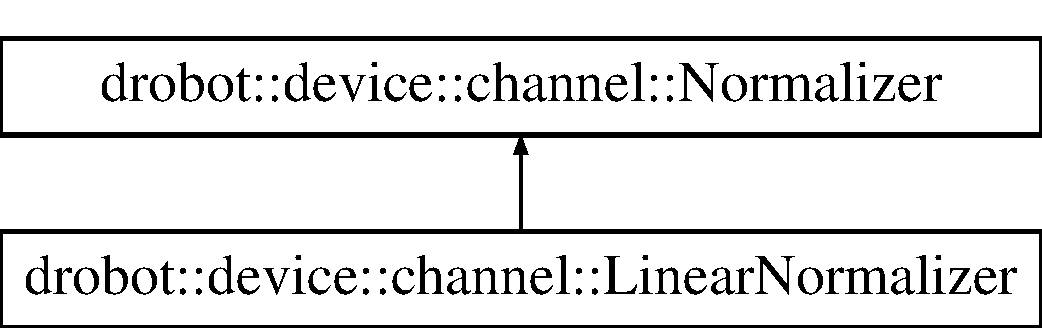
\includegraphics[height=2.000000cm]{classdrobot_1_1device_1_1channel_1_1Normalizer}
\end{center}
\end{figure}
\subsection*{Public Member Functions}
\begin{DoxyCompactItemize}
\item 
virtual double \hyperlink{classdrobot_1_1device_1_1channel_1_1Normalizer_a815d0fa0ae0f301137b7a79baff020f2}{normalize} (double value)=0
\begin{DoxyCompactList}\small\item\em normalize value to the interval from 0 to 1 \end{DoxyCompactList}\item 
virtual double \hyperlink{classdrobot_1_1device_1_1channel_1_1Normalizer_ab95ae6d2d813c70bd99efb998b78d163}{denormalize} (double value)=0
\begin{DoxyCompactList}\small\item\em denormalize value from an interval from 0 to 1 to it's original range \end{DoxyCompactList}\end{DoxyCompactItemize}


\subsection{Detailed Description}
The \hyperlink{classdrobot_1_1device_1_1channel_1_1Normalizer}{Normalizer} class. 

used to normalize a value to the interval from 0 to 1 (for use in neural networks etc) and back again. 

\subsection{Member Function Documentation}
\hypertarget{classdrobot_1_1device_1_1channel_1_1Normalizer_ab95ae6d2d813c70bd99efb998b78d163}{\index{drobot\-::device\-::channel\-::\-Normalizer@{drobot\-::device\-::channel\-::\-Normalizer}!denormalize@{denormalize}}
\index{denormalize@{denormalize}!drobot::device::channel::Normalizer@{drobot\-::device\-::channel\-::\-Normalizer}}
\subsubsection[{denormalize}]{\setlength{\rightskip}{0pt plus 5cm}virtual double drobot\-::device\-::channel\-::\-Normalizer\-::denormalize (
\begin{DoxyParamCaption}
\item[{double}]{value}
\end{DoxyParamCaption}
)\hspace{0.3cm}{\ttfamily [pure virtual]}}}\label{classdrobot_1_1device_1_1channel_1_1Normalizer_ab95ae6d2d813c70bd99efb998b78d163}


denormalize value from an interval from 0 to 1 to it's original range 


\begin{DoxyParams}{Parameters}
{\em value} & \\
\hline
\end{DoxyParams}
\begin{DoxyReturn}{Returns}
denormalized value 
\end{DoxyReturn}


Implemented in \hyperlink{classdrobot_1_1device_1_1channel_1_1LinearNormalizer_a7db474fa6bcb13adb6ffa2044d512b6d}{drobot\-::device\-::channel\-::\-Linear\-Normalizer}.

\hypertarget{classdrobot_1_1device_1_1channel_1_1Normalizer_a815d0fa0ae0f301137b7a79baff020f2}{\index{drobot\-::device\-::channel\-::\-Normalizer@{drobot\-::device\-::channel\-::\-Normalizer}!normalize@{normalize}}
\index{normalize@{normalize}!drobot::device::channel::Normalizer@{drobot\-::device\-::channel\-::\-Normalizer}}
\subsubsection[{normalize}]{\setlength{\rightskip}{0pt plus 5cm}virtual double drobot\-::device\-::channel\-::\-Normalizer\-::normalize (
\begin{DoxyParamCaption}
\item[{double}]{value}
\end{DoxyParamCaption}
)\hspace{0.3cm}{\ttfamily [pure virtual]}}}\label{classdrobot_1_1device_1_1channel_1_1Normalizer_a815d0fa0ae0f301137b7a79baff020f2}


normalize value to the interval from 0 to 1 


\begin{DoxyParams}{Parameters}
{\em value} & \\
\hline
\end{DoxyParams}
\begin{DoxyReturn}{Returns}
normalized value 
\end{DoxyReturn}


Implemented in \hyperlink{classdrobot_1_1device_1_1channel_1_1LinearNormalizer_a56e9bacaecd6b5310525d60ecd1a0f5c}{drobot\-::device\-::channel\-::\-Linear\-Normalizer}.



The documentation for this class was generated from the following file\-:\begin{DoxyCompactItemize}
\item 
src/drobot/device/channel/normalizer.\-h\end{DoxyCompactItemize}

\hypertarget{classdrobot_1_1device_1_1actuator_1_1PhidgetAdvancedBoard}{\section{drobot\-:\-:device\-:\-:actuator\-:\-:Phidget\-Advanced\-Board Class Reference}
\label{classdrobot_1_1device_1_1actuator_1_1PhidgetAdvancedBoard}\index{drobot\-::device\-::actuator\-::\-Phidget\-Advanced\-Board@{drobot\-::device\-::actuator\-::\-Phidget\-Advanced\-Board}}
}


The \hyperlink{classdrobot_1_1device_1_1actuator_1_1PhidgetAdvancedBoard}{Phidget\-Advanced\-Board} class.  




{\ttfamily \#include $<$phidgetadvancedboard.\-h$>$}

Inheritance diagram for drobot\-:\-:device\-:\-:actuator\-:\-:Phidget\-Advanced\-Board\-:\begin{figure}[H]
\begin{center}
\leavevmode
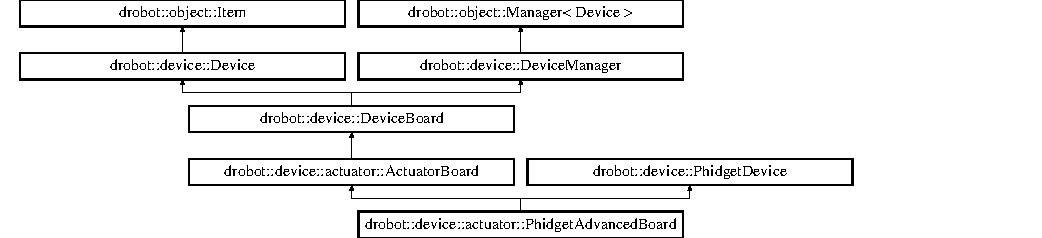
\includegraphics[height=3.196347cm]{classdrobot_1_1device_1_1actuator_1_1PhidgetAdvancedBoard}
\end{center}
\end{figure}
\subsection*{Public Member Functions}
\begin{DoxyCompactItemize}
\item 
\hyperlink{classdrobot_1_1device_1_1actuator_1_1PhidgetAdvancedBoard_a53f9277915941763356e469cd496989a}{Phidget\-Advanced\-Board} (std\-::string name)
\begin{DoxyCompactList}\small\item\em Initializes a random connected Phidget Advanced Board. \end{DoxyCompactList}\item 
\hyperlink{classdrobot_1_1device_1_1actuator_1_1PhidgetAdvancedBoard_a579c025e9bec167387fb46972c1f0f26}{Phidget\-Advanced\-Board} (std\-::string name, int serial)
\begin{DoxyCompactList}\small\item\em Initializes the Phidget Advanced Board with the given serial. \end{DoxyCompactList}\item 
\hyperlink{classdrobot_1_1device_1_1actuator_1_1PhidgetAdvancedBoard_ac84c91f6fef690afe820185e0d0c7478}{Phidget\-Advanced\-Board} (std\-::string name, C\-Phidget\-Advanced\-Servo\-Handle phidget\-Handle)
\begin{DoxyCompactList}\small\item\em Initializes a Phidget Advanced Board by the given C\-Phidget\-Advanced\-Servo\-Handle. \end{DoxyCompactList}\item 
int \hyperlink{classdrobot_1_1device_1_1actuator_1_1PhidgetAdvancedBoard_aec2cc528d8ec70e2200709d4c5ac2bf3}{get\-Max\-Actuators} ()
\item 
std\-::vector$<$ \hyperlink{classdrobot_1_1device_1_1actuator_1_1Actuator}{Actuator} $\ast$ $>$ \hyperlink{classdrobot_1_1device_1_1actuator_1_1PhidgetAdvancedBoard_a6e1564a695e5a768c14387bedfb62964}{init\-All\-Actuators} ()
\begin{DoxyCompactList}\small\item\em initializes all the connected Servo Motors and adds them to the board \end{DoxyCompactList}\item 
\hyperlink{classdrobot_1_1device_1_1actuator_1_1Actuator}{Actuator} $\ast$ \hyperlink{classdrobot_1_1device_1_1actuator_1_1PhidgetAdvancedBoard_aebc591871392ebd002fcca35b7405587}{init\-Actuator} (int index, std\-::string name)
\begin{DoxyCompactList}\small\item\em initializes the servomotor at the given index and adds it to the board \end{DoxyCompactList}\item 
\hyperlink{classdrobot_1_1device_1_1actuator_1_1Actuator}{Actuator} $\ast$ \hyperlink{classdrobot_1_1device_1_1actuator_1_1PhidgetAdvancedBoard_a1bc2bdc21b539dbf03effb0a662c318f}{init\-Actuator} (int index)
\begin{DoxyCompactList}\small\item\em initializes the servomotor at the given index and adds it to the board \end{DoxyCompactList}\end{DoxyCompactItemize}
\subsection*{Protected Member Functions}
\begin{DoxyCompactItemize}
\item 
virtual C\-Phidget\-Handle \hyperlink{classdrobot_1_1device_1_1actuator_1_1PhidgetAdvancedBoard_a67afbf98c18b80281226259f93fdb742}{get\-Phidget\-Handle} ()
\begin{DoxyCompactList}\small\item\em Must be implemented by the specific phidget device to return a C\-Phidget\-Handle struct. \end{DoxyCompactList}\end{DoxyCompactItemize}
\subsection*{Private Attributes}
\begin{DoxyCompactItemize}
\item 
\hypertarget{classdrobot_1_1device_1_1actuator_1_1PhidgetAdvancedBoard_aa7df489b3b5f23bbb1967538a1aef54a}{C\-Phidget\-Advanced\-Servo\-Handle {\bfseries \-\_\-phidget\-Handle}}\label{classdrobot_1_1device_1_1actuator_1_1PhidgetAdvancedBoard_aa7df489b3b5f23bbb1967538a1aef54a}

\end{DoxyCompactItemize}
\subsection*{Additional Inherited Members}


\subsection{Detailed Description}
The \hyperlink{classdrobot_1_1device_1_1actuator_1_1PhidgetAdvancedBoard}{Phidget\-Advanced\-Board} class. 

The Phidget Advanced Board contains Phidget Advanced Servo objects which can be initialized and used independently. 

\subsection{Constructor \& Destructor Documentation}
\hypertarget{classdrobot_1_1device_1_1actuator_1_1PhidgetAdvancedBoard_a53f9277915941763356e469cd496989a}{\index{drobot\-::device\-::actuator\-::\-Phidget\-Advanced\-Board@{drobot\-::device\-::actuator\-::\-Phidget\-Advanced\-Board}!Phidget\-Advanced\-Board@{Phidget\-Advanced\-Board}}
\index{Phidget\-Advanced\-Board@{Phidget\-Advanced\-Board}!drobot::device::actuator::PhidgetAdvancedBoard@{drobot\-::device\-::actuator\-::\-Phidget\-Advanced\-Board}}
\subsubsection[{Phidget\-Advanced\-Board}]{\setlength{\rightskip}{0pt plus 5cm}drobot\-::device\-::actuator\-::\-Phidget\-Advanced\-Board\-::\-Phidget\-Advanced\-Board (
\begin{DoxyParamCaption}
\item[{std\-::string}]{name}
\end{DoxyParamCaption}
)}}\label{classdrobot_1_1device_1_1actuator_1_1PhidgetAdvancedBoard_a53f9277915941763356e469cd496989a}


Initializes a random connected Phidget Advanced Board. 


\begin{DoxyParams}{Parameters}
{\em name} & \\
\hline
\end{DoxyParams}
\hypertarget{classdrobot_1_1device_1_1actuator_1_1PhidgetAdvancedBoard_a579c025e9bec167387fb46972c1f0f26}{\index{drobot\-::device\-::actuator\-::\-Phidget\-Advanced\-Board@{drobot\-::device\-::actuator\-::\-Phidget\-Advanced\-Board}!Phidget\-Advanced\-Board@{Phidget\-Advanced\-Board}}
\index{Phidget\-Advanced\-Board@{Phidget\-Advanced\-Board}!drobot::device::actuator::PhidgetAdvancedBoard@{drobot\-::device\-::actuator\-::\-Phidget\-Advanced\-Board}}
\subsubsection[{Phidget\-Advanced\-Board}]{\setlength{\rightskip}{0pt plus 5cm}drobot\-::device\-::actuator\-::\-Phidget\-Advanced\-Board\-::\-Phidget\-Advanced\-Board (
\begin{DoxyParamCaption}
\item[{std\-::string}]{name, }
\item[{int}]{serial}
\end{DoxyParamCaption}
)}}\label{classdrobot_1_1device_1_1actuator_1_1PhidgetAdvancedBoard_a579c025e9bec167387fb46972c1f0f26}


Initializes the Phidget Advanced Board with the given serial. 


\begin{DoxyParams}{Parameters}
{\em name} & \\
\hline
{\em serial} & \\
\hline
\end{DoxyParams}
\hypertarget{classdrobot_1_1device_1_1actuator_1_1PhidgetAdvancedBoard_ac84c91f6fef690afe820185e0d0c7478}{\index{drobot\-::device\-::actuator\-::\-Phidget\-Advanced\-Board@{drobot\-::device\-::actuator\-::\-Phidget\-Advanced\-Board}!Phidget\-Advanced\-Board@{Phidget\-Advanced\-Board}}
\index{Phidget\-Advanced\-Board@{Phidget\-Advanced\-Board}!drobot::device::actuator::PhidgetAdvancedBoard@{drobot\-::device\-::actuator\-::\-Phidget\-Advanced\-Board}}
\subsubsection[{Phidget\-Advanced\-Board}]{\setlength{\rightskip}{0pt plus 5cm}drobot\-::device\-::actuator\-::\-Phidget\-Advanced\-Board\-::\-Phidget\-Advanced\-Board (
\begin{DoxyParamCaption}
\item[{std\-::string}]{name, }
\item[{C\-Phidget\-Advanced\-Servo\-Handle}]{phidget\-Handle}
\end{DoxyParamCaption}
)}}\label{classdrobot_1_1device_1_1actuator_1_1PhidgetAdvancedBoard_ac84c91f6fef690afe820185e0d0c7478}


Initializes a Phidget Advanced Board by the given C\-Phidget\-Advanced\-Servo\-Handle. 


\begin{DoxyParams}{Parameters}
{\em name} & \\
\hline
{\em phidget\-Handle} & \\
\hline
\end{DoxyParams}


\subsection{Member Function Documentation}
\hypertarget{classdrobot_1_1device_1_1actuator_1_1PhidgetAdvancedBoard_aec2cc528d8ec70e2200709d4c5ac2bf3}{\index{drobot\-::device\-::actuator\-::\-Phidget\-Advanced\-Board@{drobot\-::device\-::actuator\-::\-Phidget\-Advanced\-Board}!get\-Max\-Actuators@{get\-Max\-Actuators}}
\index{get\-Max\-Actuators@{get\-Max\-Actuators}!drobot::device::actuator::PhidgetAdvancedBoard@{drobot\-::device\-::actuator\-::\-Phidget\-Advanced\-Board}}
\subsubsection[{get\-Max\-Actuators}]{\setlength{\rightskip}{0pt plus 5cm}int drobot\-::device\-::actuator\-::\-Phidget\-Advanced\-Board\-::get\-Max\-Actuators (
\begin{DoxyParamCaption}
{}
\end{DoxyParamCaption}
)}}\label{classdrobot_1_1device_1_1actuator_1_1PhidgetAdvancedBoard_aec2cc528d8ec70e2200709d4c5ac2bf3}
\begin{DoxyReturn}{Returns}
max number of actuators 
\end{DoxyReturn}
\hypertarget{classdrobot_1_1device_1_1actuator_1_1PhidgetAdvancedBoard_a67afbf98c18b80281226259f93fdb742}{\index{drobot\-::device\-::actuator\-::\-Phidget\-Advanced\-Board@{drobot\-::device\-::actuator\-::\-Phidget\-Advanced\-Board}!get\-Phidget\-Handle@{get\-Phidget\-Handle}}
\index{get\-Phidget\-Handle@{get\-Phidget\-Handle}!drobot::device::actuator::PhidgetAdvancedBoard@{drobot\-::device\-::actuator\-::\-Phidget\-Advanced\-Board}}
\subsubsection[{get\-Phidget\-Handle}]{\setlength{\rightskip}{0pt plus 5cm}C\-Phidget\-Handle drobot\-::device\-::actuator\-::\-Phidget\-Advanced\-Board\-::get\-Phidget\-Handle (
\begin{DoxyParamCaption}
{}
\end{DoxyParamCaption}
)\hspace{0.3cm}{\ttfamily [protected]}, {\ttfamily [virtual]}}}\label{classdrobot_1_1device_1_1actuator_1_1PhidgetAdvancedBoard_a67afbf98c18b80281226259f93fdb742}


Must be implemented by the specific phidget device to return a C\-Phidget\-Handle struct. 

\begin{DoxyReturn}{Returns}

\end{DoxyReturn}


Implements \hyperlink{classdrobot_1_1device_1_1PhidgetDevice_a0bcc3051d4a096d92b428a3166e78861}{drobot\-::device\-::\-Phidget\-Device}.

\hypertarget{classdrobot_1_1device_1_1actuator_1_1PhidgetAdvancedBoard_aebc591871392ebd002fcca35b7405587}{\index{drobot\-::device\-::actuator\-::\-Phidget\-Advanced\-Board@{drobot\-::device\-::actuator\-::\-Phidget\-Advanced\-Board}!init\-Actuator@{init\-Actuator}}
\index{init\-Actuator@{init\-Actuator}!drobot::device::actuator::PhidgetAdvancedBoard@{drobot\-::device\-::actuator\-::\-Phidget\-Advanced\-Board}}
\subsubsection[{init\-Actuator}]{\setlength{\rightskip}{0pt plus 5cm}{\bf Actuator} $\ast$ drobot\-::device\-::actuator\-::\-Phidget\-Advanced\-Board\-::init\-Actuator (
\begin{DoxyParamCaption}
\item[{int}]{index, }
\item[{std\-::string}]{name}
\end{DoxyParamCaption}
)}}\label{classdrobot_1_1device_1_1actuator_1_1PhidgetAdvancedBoard_aebc591871392ebd002fcca35b7405587}


initializes the servomotor at the given index and adds it to the board 


\begin{DoxyParams}{Parameters}
{\em index} & \\
\hline
{\em name} & of the servomotor \\
\hline
\end{DoxyParams}
\begin{DoxyReturn}{Returns}
the initialized servomotor 
\end{DoxyReturn}
\hypertarget{classdrobot_1_1device_1_1actuator_1_1PhidgetAdvancedBoard_a1bc2bdc21b539dbf03effb0a662c318f}{\index{drobot\-::device\-::actuator\-::\-Phidget\-Advanced\-Board@{drobot\-::device\-::actuator\-::\-Phidget\-Advanced\-Board}!init\-Actuator@{init\-Actuator}}
\index{init\-Actuator@{init\-Actuator}!drobot::device::actuator::PhidgetAdvancedBoard@{drobot\-::device\-::actuator\-::\-Phidget\-Advanced\-Board}}
\subsubsection[{init\-Actuator}]{\setlength{\rightskip}{0pt plus 5cm}{\bf Actuator} $\ast$ drobot\-::device\-::actuator\-::\-Phidget\-Advanced\-Board\-::init\-Actuator (
\begin{DoxyParamCaption}
\item[{int}]{index}
\end{DoxyParamCaption}
)}}\label{classdrobot_1_1device_1_1actuator_1_1PhidgetAdvancedBoard_a1bc2bdc21b539dbf03effb0a662c318f}


initializes the servomotor at the given index and adds it to the board 


\begin{DoxyParams}{Parameters}
{\em index} & \\
\hline
\end{DoxyParams}
\begin{DoxyReturn}{Returns}
the initialized servomotor 
\end{DoxyReturn}
\hypertarget{classdrobot_1_1device_1_1actuator_1_1PhidgetAdvancedBoard_a6e1564a695e5a768c14387bedfb62964}{\index{drobot\-::device\-::actuator\-::\-Phidget\-Advanced\-Board@{drobot\-::device\-::actuator\-::\-Phidget\-Advanced\-Board}!init\-All\-Actuators@{init\-All\-Actuators}}
\index{init\-All\-Actuators@{init\-All\-Actuators}!drobot::device::actuator::PhidgetAdvancedBoard@{drobot\-::device\-::actuator\-::\-Phidget\-Advanced\-Board}}
\subsubsection[{init\-All\-Actuators}]{\setlength{\rightskip}{0pt plus 5cm}std\-::vector$<$ {\bf Actuator} $\ast$ $>$ drobot\-::device\-::actuator\-::\-Phidget\-Advanced\-Board\-::init\-All\-Actuators (
\begin{DoxyParamCaption}
{}
\end{DoxyParamCaption}
)}}\label{classdrobot_1_1device_1_1actuator_1_1PhidgetAdvancedBoard_a6e1564a695e5a768c14387bedfb62964}


initializes all the connected Servo Motors and adds them to the board 

\begin{DoxyReturn}{Returns}
initialized servos 
\end{DoxyReturn}


The documentation for this class was generated from the following files\-:\begin{DoxyCompactItemize}
\item 
src/drobot/device/actuator/phidgetadvancedboard.\-h\item 
src/drobot/device/actuator/phidgetadvancedboard.\-cpp\end{DoxyCompactItemize}

\hypertarget{classdrobot_1_1device_1_1actuator_1_1PhidgetAdvancedServo}{\section{drobot\-:\-:device\-:\-:actuator\-:\-:Phidget\-Advanced\-Servo Class Reference}
\label{classdrobot_1_1device_1_1actuator_1_1PhidgetAdvancedServo}\index{drobot\-::device\-::actuator\-::\-Phidget\-Advanced\-Servo@{drobot\-::device\-::actuator\-::\-Phidget\-Advanced\-Servo}}
}


The \hyperlink{classdrobot_1_1device_1_1actuator_1_1PhidgetAdvancedServo}{Phidget\-Advanced\-Servo} class.  




{\ttfamily \#include $<$phidgetadvancedservo.\-h$>$}

Inheritance diagram for drobot\-:\-:device\-:\-:actuator\-:\-:Phidget\-Advanced\-Servo\-:\begin{figure}[H]
\begin{center}
\leavevmode
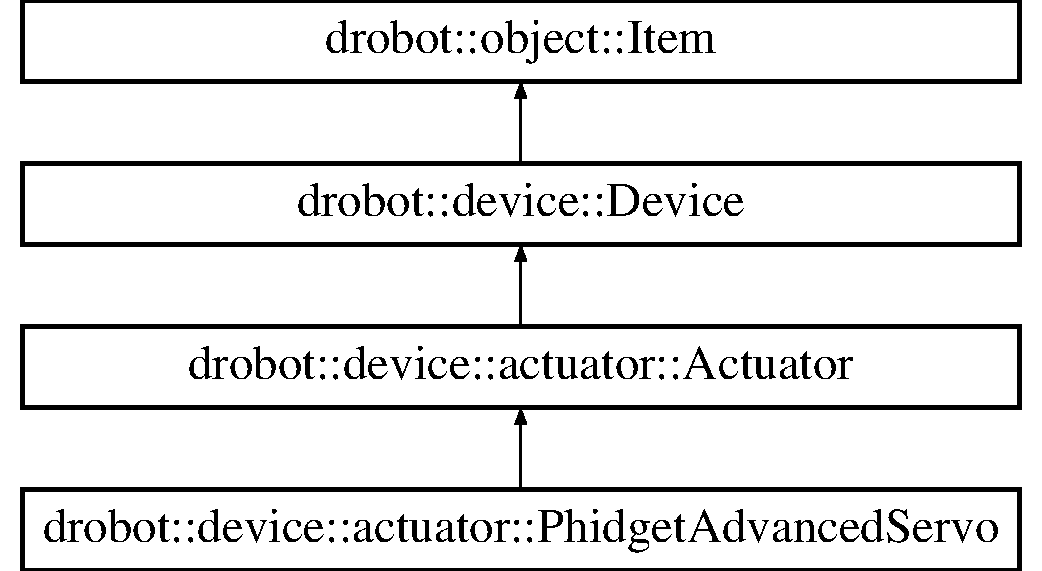
\includegraphics[height=4.000000cm]{classdrobot_1_1device_1_1actuator_1_1PhidgetAdvancedServo}
\end{center}
\end{figure}
\subsection*{Public Member Functions}
\begin{DoxyCompactItemize}
\item 
\hypertarget{classdrobot_1_1device_1_1actuator_1_1PhidgetAdvancedServo_aad070d3a5cb924e0b51d5728e8c74519}{{\bfseries Phidget\-Advanced\-Servo} (std\-::string name, C\-Phidget\-Advanced\-Servo\-Handle phidget\-Handle, int index)}\label{classdrobot_1_1device_1_1actuator_1_1PhidgetAdvancedServo_aad070d3a5cb924e0b51d5728e8c74519}

\item 
virtual void \hyperlink{classdrobot_1_1device_1_1actuator_1_1PhidgetAdvancedServo_aff32b9715c9095ed27b8b6268706b778}{enable} ()
\begin{DoxyCompactList}\small\item\em enables the device. \end{DoxyCompactList}\item 
virtual void \hyperlink{classdrobot_1_1device_1_1actuator_1_1PhidgetAdvancedServo_a62ef62d1c2052af2f2b2db1443e21c1b}{disable} ()
\begin{DoxyCompactList}\small\item\em disables the device. \end{DoxyCompactList}\item 
virtual bool \hyperlink{classdrobot_1_1device_1_1actuator_1_1PhidgetAdvancedServo_aaae782fc07c5fea70969560713c36d8c}{is\-Enabled} ()
\begin{DoxyCompactList}\small\item\em check if the device is enabled \end{DoxyCompactList}\item 
virtual double \hyperlink{classdrobot_1_1device_1_1actuator_1_1PhidgetAdvancedServo_aa3661ee800d3f130322abcd125a103ee}{get\-Position} ()
\item 
virtual void \hyperlink{classdrobot_1_1device_1_1actuator_1_1PhidgetAdvancedServo_a97cf6ba7524e113eeaa8bbe44ff3058a}{set\-Position} (double position)
\begin{DoxyCompactList}\small\item\em set motor position. The motor will always move to the last set position. \end{DoxyCompactList}\item 
virtual double \hyperlink{classdrobot_1_1device_1_1actuator_1_1PhidgetAdvancedServo_afd48104555df3fa2a8750eb19c118417}{get\-Position\-Min} ()
\item 
\hypertarget{classdrobot_1_1device_1_1actuator_1_1PhidgetAdvancedServo_ae59942ddcbe6d71a0cede7c907e4f569}{void {\bfseries set\-Position\-Min} (double position\-Min)}\label{classdrobot_1_1device_1_1actuator_1_1PhidgetAdvancedServo_ae59942ddcbe6d71a0cede7c907e4f569}

\item 
virtual double \hyperlink{classdrobot_1_1device_1_1actuator_1_1PhidgetAdvancedServo_a12335ab5360aa850bbc0a3b52028d62a}{get\-Position\-Max} ()
\item 
\hypertarget{classdrobot_1_1device_1_1actuator_1_1PhidgetAdvancedServo_a4243dcae6051395e043216cad46b2f4d}{void {\bfseries set\-Position\-Max} (double position\-Max)}\label{classdrobot_1_1device_1_1actuator_1_1PhidgetAdvancedServo_a4243dcae6051395e043216cad46b2f4d}

\item 
virtual double \hyperlink{classdrobot_1_1device_1_1actuator_1_1PhidgetAdvancedServo_ae7fa5d92717bd981d753ef03b9c32da9}{get\-Acceleration} ()
\item 
virtual void \hyperlink{classdrobot_1_1device_1_1actuator_1_1PhidgetAdvancedServo_a7c1d34496318852e20f81b145584c852}{set\-Acceleration} (double acceleration)
\begin{DoxyCompactList}\small\item\em set current acceleration \end{DoxyCompactList}\item 
virtual double \hyperlink{classdrobot_1_1device_1_1actuator_1_1PhidgetAdvancedServo_a5ff12831380c5ed0cd0ed131d0725f2b}{get\-Acceleration\-Min} ()
\item 
virtual double \hyperlink{classdrobot_1_1device_1_1actuator_1_1PhidgetAdvancedServo_a91960e941fe0813b402dbb214f41be2e}{get\-Acceleration\-Max} ()
\item 
virtual double \hyperlink{classdrobot_1_1device_1_1actuator_1_1PhidgetAdvancedServo_ade608d8b4b469ae3203fcf968f3b1455}{get\-Velocity} ()
\item 
virtual void \hyperlink{classdrobot_1_1device_1_1actuator_1_1PhidgetAdvancedServo_ae960026b28343c37bf163bd7c0f84e4b}{set\-Velocity} (double velocity)
\begin{DoxyCompactList}\small\item\em set current velocity \end{DoxyCompactList}\item 
virtual double \hyperlink{classdrobot_1_1device_1_1actuator_1_1PhidgetAdvancedServo_a77b7e687934b58aec83d19c62071bf69}{get\-Velocity\-Min} ()
\item 
virtual double \hyperlink{classdrobot_1_1device_1_1actuator_1_1PhidgetAdvancedServo_a9a0090b6dcdb7dd022687665f4ca9dd9}{get\-Velocity\-Max} ()
\item 
double \hyperlink{classdrobot_1_1device_1_1actuator_1_1PhidgetAdvancedServo_a517f67d4607950f36b67f31ff2c8f9ab}{get\-Moving\-Acceleration} ()
\begin{DoxyCompactList}\small\item\em get\-Moving\-Acceleration \end{DoxyCompactList}\item 
void \hyperlink{classdrobot_1_1device_1_1actuator_1_1PhidgetAdvancedServo_af59f97b856409b73f8ae57c717f1dfc6}{set\-Moving\-Acceleration} (double acceleration)
\begin{DoxyCompactList}\small\item\em set\-Moving\-Acceleration \end{DoxyCompactList}\item 
double \hyperlink{classdrobot_1_1device_1_1actuator_1_1PhidgetAdvancedServo_a52fd8351e208581981108f59c1b17b27}{get\-Moving\-Acceleration\-Min} ()
\begin{DoxyCompactList}\small\item\em get\-Moving\-Acceleration\-Min \end{DoxyCompactList}\item 
double \hyperlink{classdrobot_1_1device_1_1actuator_1_1PhidgetAdvancedServo_ae9c5b626332ea58cf049182b9e52eeb7}{get\-Moving\-Acceleration\-Max} ()
\begin{DoxyCompactList}\small\item\em get\-Moving\-Acceleration\-Max \end{DoxyCompactList}\item 
double \hyperlink{classdrobot_1_1device_1_1actuator_1_1PhidgetAdvancedServo_aef1b6f210ae5171468867652998cb4f3}{get\-Moving\-Velocity} ()
\begin{DoxyCompactList}\small\item\em get\-Moving\-Velocity \end{DoxyCompactList}\item 
void \hyperlink{classdrobot_1_1device_1_1actuator_1_1PhidgetAdvancedServo_a8363d8d538a9614eef2d00a25f3384a6}{set\-Moving\-Velocity} (double velocity)
\begin{DoxyCompactList}\small\item\em set\-Moving\-Velocity \end{DoxyCompactList}\item 
double \hyperlink{classdrobot_1_1device_1_1actuator_1_1PhidgetAdvancedServo_a978e8a5aac7fa6dbff354b372bc7c55f}{get\-Moving\-Velocity\-Min} ()
\begin{DoxyCompactList}\small\item\em get\-Moving\-Velocity\-Min \end{DoxyCompactList}\item 
double \hyperlink{classdrobot_1_1device_1_1actuator_1_1PhidgetAdvancedServo_a47ecef350daf66de5cef9ce4df30f668}{get\-Moving\-Velocity\-Max} ()
\begin{DoxyCompactList}\small\item\em get\-Moving\-Velocity\-Max \end{DoxyCompactList}\item 
double \hyperlink{classdrobot_1_1device_1_1actuator_1_1PhidgetAdvancedServo_ab054ba63cd62f4a4088861cb63273aee}{get\-Moving\-Velocity\-Limit} ()
\begin{DoxyCompactList}\small\item\em get\-Moving\-Velocity\-Limit \end{DoxyCompactList}\item 
void \hyperlink{classdrobot_1_1device_1_1actuator_1_1PhidgetAdvancedServo_a2d075c4f19b30e8ac705f56b4dd55603}{set\-Moving\-Velocity\-Limit} (double velocity\-Limit)
\begin{DoxyCompactList}\small\item\em set\-Moving\-Velocity\-Limit \end{DoxyCompactList}\item 
bool \hyperlink{classdrobot_1_1device_1_1actuator_1_1PhidgetAdvancedServo_a4a12cf37d6421b7e109e2c6df0efde01}{is\-Moving} ()
\begin{DoxyCompactList}\small\item\em is\-Moving \end{DoxyCompactList}\item 
\hypertarget{classdrobot_1_1device_1_1actuator_1_1PhidgetAdvancedServo_aa2dc25484399961d9b02a4cbad9b31f6}{bool {\bfseries is\-Speed\-Ramping} ()}\label{classdrobot_1_1device_1_1actuator_1_1PhidgetAdvancedServo_aa2dc25484399961d9b02a4cbad9b31f6}

\item 
\hypertarget{classdrobot_1_1device_1_1actuator_1_1PhidgetAdvancedServo_aaf173f589ee7dee578ef960919debee3}{void {\bfseries set\-Speed\-Ramping} (bool speed\-Ramping)}\label{classdrobot_1_1device_1_1actuator_1_1PhidgetAdvancedServo_aaf173f589ee7dee578ef960919debee3}

\item 
int \hyperlink{classdrobot_1_1device_1_1actuator_1_1PhidgetAdvancedServo_abab8f3244b803c8cc0c58690f21b22ed}{get\-Index} ()
\begin{DoxyCompactList}\small\item\em get\-Index \end{DoxyCompactList}\item 
double \hyperlink{classdrobot_1_1device_1_1actuator_1_1PhidgetAdvancedServo_a7594207481582d74e3921f9520b47d74}{get\-Current} ()
\begin{DoxyCompactList}\small\item\em get\-Current \end{DoxyCompactList}\end{DoxyCompactItemize}
\subsection*{Protected Member Functions}
\begin{DoxyCompactItemize}
\item 
\hypertarget{classdrobot_1_1device_1_1actuator_1_1PhidgetAdvancedServo_acdbdef2906b308868745f1d5d12559a2}{virtual C\-Phidget\-Handle \& {\bfseries get\-Phidget\-Handle} ()}\label{classdrobot_1_1device_1_1actuator_1_1PhidgetAdvancedServo_acdbdef2906b308868745f1d5d12559a2}

\end{DoxyCompactItemize}
\subsection*{Private Attributes}
\begin{DoxyCompactItemize}
\item 
\hypertarget{classdrobot_1_1device_1_1actuator_1_1PhidgetAdvancedServo_aafea126fddba6ac8b30846dbed780f08}{C\-Phidget\-Advanced\-Servo\-Handle {\bfseries \-\_\-phidget\-Handle}}\label{classdrobot_1_1device_1_1actuator_1_1PhidgetAdvancedServo_aafea126fddba6ac8b30846dbed780f08}

\item 
\hypertarget{classdrobot_1_1device_1_1actuator_1_1PhidgetAdvancedServo_ac89dae95063f7e05592b9e9534b3e6fd}{int {\bfseries \-\_\-index}}\label{classdrobot_1_1device_1_1actuator_1_1PhidgetAdvancedServo_ac89dae95063f7e05592b9e9534b3e6fd}

\end{DoxyCompactItemize}
\subsection*{Additional Inherited Members}


\subsection{Detailed Description}
The \hyperlink{classdrobot_1_1device_1_1actuator_1_1PhidgetAdvancedServo}{Phidget\-Advanced\-Servo} class. 

The \hyperlink{classdrobot_1_1device_1_1actuator_1_1PhidgetAdvancedServo}{Phidget\-Advanced\-Servo} only supports movement by setting the position. The moving\-Acceleration and moving\-Velocity properties refer to the movement initiated in this way. The acceleration and velocity properties aren't implemented by the Phidget Servo module but they can be simulated by setting the position according to the acceleration/velocity set if needed. 

\subsection{Member Function Documentation}
\hypertarget{classdrobot_1_1device_1_1actuator_1_1PhidgetAdvancedServo_a62ef62d1c2052af2f2b2db1443e21c1b}{\index{drobot\-::device\-::actuator\-::\-Phidget\-Advanced\-Servo@{drobot\-::device\-::actuator\-::\-Phidget\-Advanced\-Servo}!disable@{disable}}
\index{disable@{disable}!drobot::device::actuator::PhidgetAdvancedServo@{drobot\-::device\-::actuator\-::\-Phidget\-Advanced\-Servo}}
\subsubsection[{disable}]{\setlength{\rightskip}{0pt plus 5cm}void drobot\-::device\-::actuator\-::\-Phidget\-Advanced\-Servo\-::disable (
\begin{DoxyParamCaption}
{}
\end{DoxyParamCaption}
)\hspace{0.3cm}{\ttfamily [virtual]}}}\label{classdrobot_1_1device_1_1actuator_1_1PhidgetAdvancedServo_a62ef62d1c2052af2f2b2db1443e21c1b}


disables the device. 

This function has to be implemented by the specific device. For physical devices like actuators this method should power off the device; 

Reimplemented from \hyperlink{classdrobot_1_1device_1_1Device_a289499673ae30bd72101c68fbd04cd89}{drobot\-::device\-::\-Device}.

\hypertarget{classdrobot_1_1device_1_1actuator_1_1PhidgetAdvancedServo_aff32b9715c9095ed27b8b6268706b778}{\index{drobot\-::device\-::actuator\-::\-Phidget\-Advanced\-Servo@{drobot\-::device\-::actuator\-::\-Phidget\-Advanced\-Servo}!enable@{enable}}
\index{enable@{enable}!drobot::device::actuator::PhidgetAdvancedServo@{drobot\-::device\-::actuator\-::\-Phidget\-Advanced\-Servo}}
\subsubsection[{enable}]{\setlength{\rightskip}{0pt plus 5cm}void drobot\-::device\-::actuator\-::\-Phidget\-Advanced\-Servo\-::enable (
\begin{DoxyParamCaption}
{}
\end{DoxyParamCaption}
)\hspace{0.3cm}{\ttfamily [virtual]}}}\label{classdrobot_1_1device_1_1actuator_1_1PhidgetAdvancedServo_aff32b9715c9095ed27b8b6268706b778}


enables the device. 

This function has to be implemented by the specific device. For physical devices like actuators this method should power on the device. 

Reimplemented from \hyperlink{classdrobot_1_1device_1_1Device_a0c28785ff2e79f99b8e9eaefe6749f2b}{drobot\-::device\-::\-Device}.

\hypertarget{classdrobot_1_1device_1_1actuator_1_1PhidgetAdvancedServo_ae7fa5d92717bd981d753ef03b9c32da9}{\index{drobot\-::device\-::actuator\-::\-Phidget\-Advanced\-Servo@{drobot\-::device\-::actuator\-::\-Phidget\-Advanced\-Servo}!get\-Acceleration@{get\-Acceleration}}
\index{get\-Acceleration@{get\-Acceleration}!drobot::device::actuator::PhidgetAdvancedServo@{drobot\-::device\-::actuator\-::\-Phidget\-Advanced\-Servo}}
\subsubsection[{get\-Acceleration}]{\setlength{\rightskip}{0pt plus 5cm}double drobot\-::device\-::actuator\-::\-Phidget\-Advanced\-Servo\-::get\-Acceleration (
\begin{DoxyParamCaption}
{}
\end{DoxyParamCaption}
)\hspace{0.3cm}{\ttfamily [virtual]}}}\label{classdrobot_1_1device_1_1actuator_1_1PhidgetAdvancedServo_ae7fa5d92717bd981d753ef03b9c32da9}
\begin{DoxyReturn}{Returns}
current acceleration 
\end{DoxyReturn}


Implements \hyperlink{classdrobot_1_1device_1_1actuator_1_1Actuator_a9dd6e74032417e5a84946925c655047c}{drobot\-::device\-::actuator\-::\-Actuator}.

\hypertarget{classdrobot_1_1device_1_1actuator_1_1PhidgetAdvancedServo_a91960e941fe0813b402dbb214f41be2e}{\index{drobot\-::device\-::actuator\-::\-Phidget\-Advanced\-Servo@{drobot\-::device\-::actuator\-::\-Phidget\-Advanced\-Servo}!get\-Acceleration\-Max@{get\-Acceleration\-Max}}
\index{get\-Acceleration\-Max@{get\-Acceleration\-Max}!drobot::device::actuator::PhidgetAdvancedServo@{drobot\-::device\-::actuator\-::\-Phidget\-Advanced\-Servo}}
\subsubsection[{get\-Acceleration\-Max}]{\setlength{\rightskip}{0pt plus 5cm}double drobot\-::device\-::actuator\-::\-Phidget\-Advanced\-Servo\-::get\-Acceleration\-Max (
\begin{DoxyParamCaption}
{}
\end{DoxyParamCaption}
)\hspace{0.3cm}{\ttfamily [virtual]}}}\label{classdrobot_1_1device_1_1actuator_1_1PhidgetAdvancedServo_a91960e941fe0813b402dbb214f41be2e}
\begin{DoxyReturn}{Returns}
maximal possible acceleration 
\end{DoxyReturn}


Implements \hyperlink{classdrobot_1_1device_1_1actuator_1_1Actuator_a74e4fc92b8a3661ccbc44435411fbfca}{drobot\-::device\-::actuator\-::\-Actuator}.

\hypertarget{classdrobot_1_1device_1_1actuator_1_1PhidgetAdvancedServo_a5ff12831380c5ed0cd0ed131d0725f2b}{\index{drobot\-::device\-::actuator\-::\-Phidget\-Advanced\-Servo@{drobot\-::device\-::actuator\-::\-Phidget\-Advanced\-Servo}!get\-Acceleration\-Min@{get\-Acceleration\-Min}}
\index{get\-Acceleration\-Min@{get\-Acceleration\-Min}!drobot::device::actuator::PhidgetAdvancedServo@{drobot\-::device\-::actuator\-::\-Phidget\-Advanced\-Servo}}
\subsubsection[{get\-Acceleration\-Min}]{\setlength{\rightskip}{0pt plus 5cm}double drobot\-::device\-::actuator\-::\-Phidget\-Advanced\-Servo\-::get\-Acceleration\-Min (
\begin{DoxyParamCaption}
{}
\end{DoxyParamCaption}
)\hspace{0.3cm}{\ttfamily [virtual]}}}\label{classdrobot_1_1device_1_1actuator_1_1PhidgetAdvancedServo_a5ff12831380c5ed0cd0ed131d0725f2b}
\begin{DoxyReturn}{Returns}
minimal possible acceleration 
\end{DoxyReturn}


Implements \hyperlink{classdrobot_1_1device_1_1actuator_1_1Actuator_a16714b00aafdd84affaf9bc3a8383c48}{drobot\-::device\-::actuator\-::\-Actuator}.

\hypertarget{classdrobot_1_1device_1_1actuator_1_1PhidgetAdvancedServo_a7594207481582d74e3921f9520b47d74}{\index{drobot\-::device\-::actuator\-::\-Phidget\-Advanced\-Servo@{drobot\-::device\-::actuator\-::\-Phidget\-Advanced\-Servo}!get\-Current@{get\-Current}}
\index{get\-Current@{get\-Current}!drobot::device::actuator::PhidgetAdvancedServo@{drobot\-::device\-::actuator\-::\-Phidget\-Advanced\-Servo}}
\subsubsection[{get\-Current}]{\setlength{\rightskip}{0pt plus 5cm}double drobot\-::device\-::actuator\-::\-Phidget\-Advanced\-Servo\-::get\-Current (
\begin{DoxyParamCaption}
{}
\end{DoxyParamCaption}
)}}\label{classdrobot_1_1device_1_1actuator_1_1PhidgetAdvancedServo_a7594207481582d74e3921f9520b47d74}


get\-Current 

\begin{DoxyReturn}{Returns}
amount of current the motor is using 
\end{DoxyReturn}
\hypertarget{classdrobot_1_1device_1_1actuator_1_1PhidgetAdvancedServo_abab8f3244b803c8cc0c58690f21b22ed}{\index{drobot\-::device\-::actuator\-::\-Phidget\-Advanced\-Servo@{drobot\-::device\-::actuator\-::\-Phidget\-Advanced\-Servo}!get\-Index@{get\-Index}}
\index{get\-Index@{get\-Index}!drobot::device::actuator::PhidgetAdvancedServo@{drobot\-::device\-::actuator\-::\-Phidget\-Advanced\-Servo}}
\subsubsection[{get\-Index}]{\setlength{\rightskip}{0pt plus 5cm}int drobot\-::device\-::actuator\-::\-Phidget\-Advanced\-Servo\-::get\-Index (
\begin{DoxyParamCaption}
{}
\end{DoxyParamCaption}
)}}\label{classdrobot_1_1device_1_1actuator_1_1PhidgetAdvancedServo_abab8f3244b803c8cc0c58690f21b22ed}


get\-Index 

\begin{DoxyReturn}{Returns}
index of the motor in the servo board 
\end{DoxyReturn}
\hypertarget{classdrobot_1_1device_1_1actuator_1_1PhidgetAdvancedServo_a517f67d4607950f36b67f31ff2c8f9ab}{\index{drobot\-::device\-::actuator\-::\-Phidget\-Advanced\-Servo@{drobot\-::device\-::actuator\-::\-Phidget\-Advanced\-Servo}!get\-Moving\-Acceleration@{get\-Moving\-Acceleration}}
\index{get\-Moving\-Acceleration@{get\-Moving\-Acceleration}!drobot::device::actuator::PhidgetAdvancedServo@{drobot\-::device\-::actuator\-::\-Phidget\-Advanced\-Servo}}
\subsubsection[{get\-Moving\-Acceleration}]{\setlength{\rightskip}{0pt plus 5cm}double drobot\-::device\-::actuator\-::\-Phidget\-Advanced\-Servo\-::get\-Moving\-Acceleration (
\begin{DoxyParamCaption}
{}
\end{DoxyParamCaption}
)}}\label{classdrobot_1_1device_1_1actuator_1_1PhidgetAdvancedServo_a517f67d4607950f36b67f31ff2c8f9ab}


get\-Moving\-Acceleration 

\begin{DoxyReturn}{Returns}
the acceleration of the movement 
\end{DoxyReturn}
\hypertarget{classdrobot_1_1device_1_1actuator_1_1PhidgetAdvancedServo_ae9c5b626332ea58cf049182b9e52eeb7}{\index{drobot\-::device\-::actuator\-::\-Phidget\-Advanced\-Servo@{drobot\-::device\-::actuator\-::\-Phidget\-Advanced\-Servo}!get\-Moving\-Acceleration\-Max@{get\-Moving\-Acceleration\-Max}}
\index{get\-Moving\-Acceleration\-Max@{get\-Moving\-Acceleration\-Max}!drobot::device::actuator::PhidgetAdvancedServo@{drobot\-::device\-::actuator\-::\-Phidget\-Advanced\-Servo}}
\subsubsection[{get\-Moving\-Acceleration\-Max}]{\setlength{\rightskip}{0pt plus 5cm}double drobot\-::device\-::actuator\-::\-Phidget\-Advanced\-Servo\-::get\-Moving\-Acceleration\-Max (
\begin{DoxyParamCaption}
{}
\end{DoxyParamCaption}
)}}\label{classdrobot_1_1device_1_1actuator_1_1PhidgetAdvancedServo_ae9c5b626332ea58cf049182b9e52eeb7}


get\-Moving\-Acceleration\-Max 

\begin{DoxyReturn}{Returns}
maximum acceleration 
\end{DoxyReturn}
\hypertarget{classdrobot_1_1device_1_1actuator_1_1PhidgetAdvancedServo_a52fd8351e208581981108f59c1b17b27}{\index{drobot\-::device\-::actuator\-::\-Phidget\-Advanced\-Servo@{drobot\-::device\-::actuator\-::\-Phidget\-Advanced\-Servo}!get\-Moving\-Acceleration\-Min@{get\-Moving\-Acceleration\-Min}}
\index{get\-Moving\-Acceleration\-Min@{get\-Moving\-Acceleration\-Min}!drobot::device::actuator::PhidgetAdvancedServo@{drobot\-::device\-::actuator\-::\-Phidget\-Advanced\-Servo}}
\subsubsection[{get\-Moving\-Acceleration\-Min}]{\setlength{\rightskip}{0pt plus 5cm}double drobot\-::device\-::actuator\-::\-Phidget\-Advanced\-Servo\-::get\-Moving\-Acceleration\-Min (
\begin{DoxyParamCaption}
{}
\end{DoxyParamCaption}
)}}\label{classdrobot_1_1device_1_1actuator_1_1PhidgetAdvancedServo_a52fd8351e208581981108f59c1b17b27}


get\-Moving\-Acceleration\-Min 

\begin{DoxyReturn}{Returns}
minimum acceleration 
\end{DoxyReturn}
\hypertarget{classdrobot_1_1device_1_1actuator_1_1PhidgetAdvancedServo_aef1b6f210ae5171468867652998cb4f3}{\index{drobot\-::device\-::actuator\-::\-Phidget\-Advanced\-Servo@{drobot\-::device\-::actuator\-::\-Phidget\-Advanced\-Servo}!get\-Moving\-Velocity@{get\-Moving\-Velocity}}
\index{get\-Moving\-Velocity@{get\-Moving\-Velocity}!drobot::device::actuator::PhidgetAdvancedServo@{drobot\-::device\-::actuator\-::\-Phidget\-Advanced\-Servo}}
\subsubsection[{get\-Moving\-Velocity}]{\setlength{\rightskip}{0pt plus 5cm}double drobot\-::device\-::actuator\-::\-Phidget\-Advanced\-Servo\-::get\-Moving\-Velocity (
\begin{DoxyParamCaption}
{}
\end{DoxyParamCaption}
)}}\label{classdrobot_1_1device_1_1actuator_1_1PhidgetAdvancedServo_aef1b6f210ae5171468867652998cb4f3}


get\-Moving\-Velocity 

\begin{DoxyReturn}{Returns}
the velocity of the movement 
\end{DoxyReturn}
\hypertarget{classdrobot_1_1device_1_1actuator_1_1PhidgetAdvancedServo_ab054ba63cd62f4a4088861cb63273aee}{\index{drobot\-::device\-::actuator\-::\-Phidget\-Advanced\-Servo@{drobot\-::device\-::actuator\-::\-Phidget\-Advanced\-Servo}!get\-Moving\-Velocity\-Limit@{get\-Moving\-Velocity\-Limit}}
\index{get\-Moving\-Velocity\-Limit@{get\-Moving\-Velocity\-Limit}!drobot::device::actuator::PhidgetAdvancedServo@{drobot\-::device\-::actuator\-::\-Phidget\-Advanced\-Servo}}
\subsubsection[{get\-Moving\-Velocity\-Limit}]{\setlength{\rightskip}{0pt plus 5cm}double drobot\-::device\-::actuator\-::\-Phidget\-Advanced\-Servo\-::get\-Moving\-Velocity\-Limit (
\begin{DoxyParamCaption}
{}
\end{DoxyParamCaption}
)}}\label{classdrobot_1_1device_1_1actuator_1_1PhidgetAdvancedServo_ab054ba63cd62f4a4088861cb63273aee}


get\-Moving\-Velocity\-Limit 

\begin{DoxyReturn}{Returns}
velocity 
\end{DoxyReturn}
\hypertarget{classdrobot_1_1device_1_1actuator_1_1PhidgetAdvancedServo_a47ecef350daf66de5cef9ce4df30f668}{\index{drobot\-::device\-::actuator\-::\-Phidget\-Advanced\-Servo@{drobot\-::device\-::actuator\-::\-Phidget\-Advanced\-Servo}!get\-Moving\-Velocity\-Max@{get\-Moving\-Velocity\-Max}}
\index{get\-Moving\-Velocity\-Max@{get\-Moving\-Velocity\-Max}!drobot::device::actuator::PhidgetAdvancedServo@{drobot\-::device\-::actuator\-::\-Phidget\-Advanced\-Servo}}
\subsubsection[{get\-Moving\-Velocity\-Max}]{\setlength{\rightskip}{0pt plus 5cm}double drobot\-::device\-::actuator\-::\-Phidget\-Advanced\-Servo\-::get\-Moving\-Velocity\-Max (
\begin{DoxyParamCaption}
{}
\end{DoxyParamCaption}
)}}\label{classdrobot_1_1device_1_1actuator_1_1PhidgetAdvancedServo_a47ecef350daf66de5cef9ce4df30f668}


get\-Moving\-Velocity\-Max 

\begin{DoxyReturn}{Returns}
maximum possible velocity of the servo device 
\end{DoxyReturn}
\hypertarget{classdrobot_1_1device_1_1actuator_1_1PhidgetAdvancedServo_a978e8a5aac7fa6dbff354b372bc7c55f}{\index{drobot\-::device\-::actuator\-::\-Phidget\-Advanced\-Servo@{drobot\-::device\-::actuator\-::\-Phidget\-Advanced\-Servo}!get\-Moving\-Velocity\-Min@{get\-Moving\-Velocity\-Min}}
\index{get\-Moving\-Velocity\-Min@{get\-Moving\-Velocity\-Min}!drobot::device::actuator::PhidgetAdvancedServo@{drobot\-::device\-::actuator\-::\-Phidget\-Advanced\-Servo}}
\subsubsection[{get\-Moving\-Velocity\-Min}]{\setlength{\rightskip}{0pt plus 5cm}double drobot\-::device\-::actuator\-::\-Phidget\-Advanced\-Servo\-::get\-Moving\-Velocity\-Min (
\begin{DoxyParamCaption}
{}
\end{DoxyParamCaption}
)}}\label{classdrobot_1_1device_1_1actuator_1_1PhidgetAdvancedServo_a978e8a5aac7fa6dbff354b372bc7c55f}


get\-Moving\-Velocity\-Min 

\begin{DoxyReturn}{Returns}
minimum possible velocity of the servo device 
\end{DoxyReturn}
\hypertarget{classdrobot_1_1device_1_1actuator_1_1PhidgetAdvancedServo_aa3661ee800d3f130322abcd125a103ee}{\index{drobot\-::device\-::actuator\-::\-Phidget\-Advanced\-Servo@{drobot\-::device\-::actuator\-::\-Phidget\-Advanced\-Servo}!get\-Position@{get\-Position}}
\index{get\-Position@{get\-Position}!drobot::device::actuator::PhidgetAdvancedServo@{drobot\-::device\-::actuator\-::\-Phidget\-Advanced\-Servo}}
\subsubsection[{get\-Position}]{\setlength{\rightskip}{0pt plus 5cm}double drobot\-::device\-::actuator\-::\-Phidget\-Advanced\-Servo\-::get\-Position (
\begin{DoxyParamCaption}
{}
\end{DoxyParamCaption}
)\hspace{0.3cm}{\ttfamily [virtual]}}}\label{classdrobot_1_1device_1_1actuator_1_1PhidgetAdvancedServo_aa3661ee800d3f130322abcd125a103ee}
\begin{DoxyReturn}{Returns}
current motor position 
\end{DoxyReturn}


Implements \hyperlink{classdrobot_1_1device_1_1actuator_1_1Actuator_aea525e325f2eb2058a37db3e014bb872}{drobot\-::device\-::actuator\-::\-Actuator}.

\hypertarget{classdrobot_1_1device_1_1actuator_1_1PhidgetAdvancedServo_a12335ab5360aa850bbc0a3b52028d62a}{\index{drobot\-::device\-::actuator\-::\-Phidget\-Advanced\-Servo@{drobot\-::device\-::actuator\-::\-Phidget\-Advanced\-Servo}!get\-Position\-Max@{get\-Position\-Max}}
\index{get\-Position\-Max@{get\-Position\-Max}!drobot::device::actuator::PhidgetAdvancedServo@{drobot\-::device\-::actuator\-::\-Phidget\-Advanced\-Servo}}
\subsubsection[{get\-Position\-Max}]{\setlength{\rightskip}{0pt plus 5cm}double drobot\-::device\-::actuator\-::\-Phidget\-Advanced\-Servo\-::get\-Position\-Max (
\begin{DoxyParamCaption}
{}
\end{DoxyParamCaption}
)\hspace{0.3cm}{\ttfamily [virtual]}}}\label{classdrobot_1_1device_1_1actuator_1_1PhidgetAdvancedServo_a12335ab5360aa850bbc0a3b52028d62a}
\begin{DoxyReturn}{Returns}
minimal possible position 
\end{DoxyReturn}


Implements \hyperlink{classdrobot_1_1device_1_1actuator_1_1Actuator_a3a02ed0a72f8ab360748df0d9872eeb3}{drobot\-::device\-::actuator\-::\-Actuator}.

\hypertarget{classdrobot_1_1device_1_1actuator_1_1PhidgetAdvancedServo_afd48104555df3fa2a8750eb19c118417}{\index{drobot\-::device\-::actuator\-::\-Phidget\-Advanced\-Servo@{drobot\-::device\-::actuator\-::\-Phidget\-Advanced\-Servo}!get\-Position\-Min@{get\-Position\-Min}}
\index{get\-Position\-Min@{get\-Position\-Min}!drobot::device::actuator::PhidgetAdvancedServo@{drobot\-::device\-::actuator\-::\-Phidget\-Advanced\-Servo}}
\subsubsection[{get\-Position\-Min}]{\setlength{\rightskip}{0pt plus 5cm}double drobot\-::device\-::actuator\-::\-Phidget\-Advanced\-Servo\-::get\-Position\-Min (
\begin{DoxyParamCaption}
{}
\end{DoxyParamCaption}
)\hspace{0.3cm}{\ttfamily [virtual]}}}\label{classdrobot_1_1device_1_1actuator_1_1PhidgetAdvancedServo_afd48104555df3fa2a8750eb19c118417}
\begin{DoxyReturn}{Returns}
maximal possible position 
\end{DoxyReturn}


Implements \hyperlink{classdrobot_1_1device_1_1actuator_1_1Actuator_a7a4c195442470d46275f62446e5d2535}{drobot\-::device\-::actuator\-::\-Actuator}.

\hypertarget{classdrobot_1_1device_1_1actuator_1_1PhidgetAdvancedServo_ade608d8b4b469ae3203fcf968f3b1455}{\index{drobot\-::device\-::actuator\-::\-Phidget\-Advanced\-Servo@{drobot\-::device\-::actuator\-::\-Phidget\-Advanced\-Servo}!get\-Velocity@{get\-Velocity}}
\index{get\-Velocity@{get\-Velocity}!drobot::device::actuator::PhidgetAdvancedServo@{drobot\-::device\-::actuator\-::\-Phidget\-Advanced\-Servo}}
\subsubsection[{get\-Velocity}]{\setlength{\rightskip}{0pt plus 5cm}double drobot\-::device\-::actuator\-::\-Phidget\-Advanced\-Servo\-::get\-Velocity (
\begin{DoxyParamCaption}
{}
\end{DoxyParamCaption}
)\hspace{0.3cm}{\ttfamily [virtual]}}}\label{classdrobot_1_1device_1_1actuator_1_1PhidgetAdvancedServo_ade608d8b4b469ae3203fcf968f3b1455}
\begin{DoxyReturn}{Returns}
current velocity 
\end{DoxyReturn}


Implements \hyperlink{classdrobot_1_1device_1_1actuator_1_1Actuator_a9fea4e618e465cbcc9a207740dbc5410}{drobot\-::device\-::actuator\-::\-Actuator}.

\hypertarget{classdrobot_1_1device_1_1actuator_1_1PhidgetAdvancedServo_a9a0090b6dcdb7dd022687665f4ca9dd9}{\index{drobot\-::device\-::actuator\-::\-Phidget\-Advanced\-Servo@{drobot\-::device\-::actuator\-::\-Phidget\-Advanced\-Servo}!get\-Velocity\-Max@{get\-Velocity\-Max}}
\index{get\-Velocity\-Max@{get\-Velocity\-Max}!drobot::device::actuator::PhidgetAdvancedServo@{drobot\-::device\-::actuator\-::\-Phidget\-Advanced\-Servo}}
\subsubsection[{get\-Velocity\-Max}]{\setlength{\rightskip}{0pt plus 5cm}double drobot\-::device\-::actuator\-::\-Phidget\-Advanced\-Servo\-::get\-Velocity\-Max (
\begin{DoxyParamCaption}
{}
\end{DoxyParamCaption}
)\hspace{0.3cm}{\ttfamily [virtual]}}}\label{classdrobot_1_1device_1_1actuator_1_1PhidgetAdvancedServo_a9a0090b6dcdb7dd022687665f4ca9dd9}
\begin{DoxyReturn}{Returns}
maximal possible velocity 
\end{DoxyReturn}


Implements \hyperlink{classdrobot_1_1device_1_1actuator_1_1Actuator_a5a018f4e240fb1a483307c03a7662f3d}{drobot\-::device\-::actuator\-::\-Actuator}.

\hypertarget{classdrobot_1_1device_1_1actuator_1_1PhidgetAdvancedServo_a77b7e687934b58aec83d19c62071bf69}{\index{drobot\-::device\-::actuator\-::\-Phidget\-Advanced\-Servo@{drobot\-::device\-::actuator\-::\-Phidget\-Advanced\-Servo}!get\-Velocity\-Min@{get\-Velocity\-Min}}
\index{get\-Velocity\-Min@{get\-Velocity\-Min}!drobot::device::actuator::PhidgetAdvancedServo@{drobot\-::device\-::actuator\-::\-Phidget\-Advanced\-Servo}}
\subsubsection[{get\-Velocity\-Min}]{\setlength{\rightskip}{0pt plus 5cm}double drobot\-::device\-::actuator\-::\-Phidget\-Advanced\-Servo\-::get\-Velocity\-Min (
\begin{DoxyParamCaption}
{}
\end{DoxyParamCaption}
)\hspace{0.3cm}{\ttfamily [virtual]}}}\label{classdrobot_1_1device_1_1actuator_1_1PhidgetAdvancedServo_a77b7e687934b58aec83d19c62071bf69}
\begin{DoxyReturn}{Returns}
minimal possible velocity 
\end{DoxyReturn}


Implements \hyperlink{classdrobot_1_1device_1_1actuator_1_1Actuator_a3ddbc25d10ca91b0719ad8b3b6220948}{drobot\-::device\-::actuator\-::\-Actuator}.

\hypertarget{classdrobot_1_1device_1_1actuator_1_1PhidgetAdvancedServo_aaae782fc07c5fea70969560713c36d8c}{\index{drobot\-::device\-::actuator\-::\-Phidget\-Advanced\-Servo@{drobot\-::device\-::actuator\-::\-Phidget\-Advanced\-Servo}!is\-Enabled@{is\-Enabled}}
\index{is\-Enabled@{is\-Enabled}!drobot::device::actuator::PhidgetAdvancedServo@{drobot\-::device\-::actuator\-::\-Phidget\-Advanced\-Servo}}
\subsubsection[{is\-Enabled}]{\setlength{\rightskip}{0pt plus 5cm}bool drobot\-::device\-::actuator\-::\-Phidget\-Advanced\-Servo\-::is\-Enabled (
\begin{DoxyParamCaption}
{}
\end{DoxyParamCaption}
)\hspace{0.3cm}{\ttfamily [virtual]}}}\label{classdrobot_1_1device_1_1actuator_1_1PhidgetAdvancedServo_aaae782fc07c5fea70969560713c36d8c}


check if the device is enabled 

\begin{DoxyReturn}{Returns}
true if enabled else false
\end{DoxyReturn}
While the \hyperlink{classdrobot_1_1robot_1_1Robot}{drobot\-::robot\-::\-Robot} is running this property is checked to see whether the device should be used or not. 

Implements \hyperlink{classdrobot_1_1device_1_1Device_aa5b7eac8638d0d2d5ee9bf10607b100e}{drobot\-::device\-::\-Device}.

\hypertarget{classdrobot_1_1device_1_1actuator_1_1PhidgetAdvancedServo_a4a12cf37d6421b7e109e2c6df0efde01}{\index{drobot\-::device\-::actuator\-::\-Phidget\-Advanced\-Servo@{drobot\-::device\-::actuator\-::\-Phidget\-Advanced\-Servo}!is\-Moving@{is\-Moving}}
\index{is\-Moving@{is\-Moving}!drobot::device::actuator::PhidgetAdvancedServo@{drobot\-::device\-::actuator\-::\-Phidget\-Advanced\-Servo}}
\subsubsection[{is\-Moving}]{\setlength{\rightskip}{0pt plus 5cm}bool drobot\-::device\-::actuator\-::\-Phidget\-Advanced\-Servo\-::is\-Moving (
\begin{DoxyParamCaption}
{}
\end{DoxyParamCaption}
)}}\label{classdrobot_1_1device_1_1actuator_1_1PhidgetAdvancedServo_a4a12cf37d6421b7e109e2c6df0efde01}


is\-Moving 

\begin{DoxyReturn}{Returns}
true if motor is moving. false otherwhise 
\end{DoxyReturn}
\hypertarget{classdrobot_1_1device_1_1actuator_1_1PhidgetAdvancedServo_a7c1d34496318852e20f81b145584c852}{\index{drobot\-::device\-::actuator\-::\-Phidget\-Advanced\-Servo@{drobot\-::device\-::actuator\-::\-Phidget\-Advanced\-Servo}!set\-Acceleration@{set\-Acceleration}}
\index{set\-Acceleration@{set\-Acceleration}!drobot::device::actuator::PhidgetAdvancedServo@{drobot\-::device\-::actuator\-::\-Phidget\-Advanced\-Servo}}
\subsubsection[{set\-Acceleration}]{\setlength{\rightskip}{0pt plus 5cm}void drobot\-::device\-::actuator\-::\-Phidget\-Advanced\-Servo\-::set\-Acceleration (
\begin{DoxyParamCaption}
\item[{double}]{acceleration}
\end{DoxyParamCaption}
)\hspace{0.3cm}{\ttfamily [virtual]}}}\label{classdrobot_1_1device_1_1actuator_1_1PhidgetAdvancedServo_a7c1d34496318852e20f81b145584c852}


set current acceleration 


\begin{DoxyParams}{Parameters}
{\em acceleration} & \\
\hline
\end{DoxyParams}


Implements \hyperlink{classdrobot_1_1device_1_1actuator_1_1Actuator_a4056ed7c5038c86cd1ed24425a8e2d87}{drobot\-::device\-::actuator\-::\-Actuator}.

\hypertarget{classdrobot_1_1device_1_1actuator_1_1PhidgetAdvancedServo_af59f97b856409b73f8ae57c717f1dfc6}{\index{drobot\-::device\-::actuator\-::\-Phidget\-Advanced\-Servo@{drobot\-::device\-::actuator\-::\-Phidget\-Advanced\-Servo}!set\-Moving\-Acceleration@{set\-Moving\-Acceleration}}
\index{set\-Moving\-Acceleration@{set\-Moving\-Acceleration}!drobot::device::actuator::PhidgetAdvancedServo@{drobot\-::device\-::actuator\-::\-Phidget\-Advanced\-Servo}}
\subsubsection[{set\-Moving\-Acceleration}]{\setlength{\rightskip}{0pt plus 5cm}void drobot\-::device\-::actuator\-::\-Phidget\-Advanced\-Servo\-::set\-Moving\-Acceleration (
\begin{DoxyParamCaption}
\item[{double}]{acceleration}
\end{DoxyParamCaption}
)}}\label{classdrobot_1_1device_1_1actuator_1_1PhidgetAdvancedServo_af59f97b856409b73f8ae57c717f1dfc6}


set\-Moving\-Acceleration 

this property controls the acceleration of the movement if the servo is set to a new position 
\begin{DoxyParams}{Parameters}
{\em acceleration} & \\
\hline
\end{DoxyParams}
\hypertarget{classdrobot_1_1device_1_1actuator_1_1PhidgetAdvancedServo_a8363d8d538a9614eef2d00a25f3384a6}{\index{drobot\-::device\-::actuator\-::\-Phidget\-Advanced\-Servo@{drobot\-::device\-::actuator\-::\-Phidget\-Advanced\-Servo}!set\-Moving\-Velocity@{set\-Moving\-Velocity}}
\index{set\-Moving\-Velocity@{set\-Moving\-Velocity}!drobot::device::actuator::PhidgetAdvancedServo@{drobot\-::device\-::actuator\-::\-Phidget\-Advanced\-Servo}}
\subsubsection[{set\-Moving\-Velocity}]{\setlength{\rightskip}{0pt plus 5cm}void drobot\-::device\-::actuator\-::\-Phidget\-Advanced\-Servo\-::set\-Moving\-Velocity (
\begin{DoxyParamCaption}
\item[{double}]{velocity}
\end{DoxyParamCaption}
)}}\label{classdrobot_1_1device_1_1actuator_1_1PhidgetAdvancedServo_a8363d8d538a9614eef2d00a25f3384a6}


set\-Moving\-Velocity 

this property controls the velocity of the movement if the servo is set to a new position 
\begin{DoxyParams}{Parameters}
{\em velocity} & \\
\hline
\end{DoxyParams}
\hypertarget{classdrobot_1_1device_1_1actuator_1_1PhidgetAdvancedServo_a2d075c4f19b30e8ac705f56b4dd55603}{\index{drobot\-::device\-::actuator\-::\-Phidget\-Advanced\-Servo@{drobot\-::device\-::actuator\-::\-Phidget\-Advanced\-Servo}!set\-Moving\-Velocity\-Limit@{set\-Moving\-Velocity\-Limit}}
\index{set\-Moving\-Velocity\-Limit@{set\-Moving\-Velocity\-Limit}!drobot::device::actuator::PhidgetAdvancedServo@{drobot\-::device\-::actuator\-::\-Phidget\-Advanced\-Servo}}
\subsubsection[{set\-Moving\-Velocity\-Limit}]{\setlength{\rightskip}{0pt plus 5cm}void drobot\-::device\-::actuator\-::\-Phidget\-Advanced\-Servo\-::set\-Moving\-Velocity\-Limit (
\begin{DoxyParamCaption}
\item[{double}]{velocity\-Limit}
\end{DoxyParamCaption}
)}}\label{classdrobot_1_1device_1_1actuator_1_1PhidgetAdvancedServo_a2d075c4f19b30e8ac705f56b4dd55603}


set\-Moving\-Velocity\-Limit 


\begin{DoxyParams}{Parameters}
{\em velocity\-Limit} & \\
\hline
\end{DoxyParams}
\hypertarget{classdrobot_1_1device_1_1actuator_1_1PhidgetAdvancedServo_a97cf6ba7524e113eeaa8bbe44ff3058a}{\index{drobot\-::device\-::actuator\-::\-Phidget\-Advanced\-Servo@{drobot\-::device\-::actuator\-::\-Phidget\-Advanced\-Servo}!set\-Position@{set\-Position}}
\index{set\-Position@{set\-Position}!drobot::device::actuator::PhidgetAdvancedServo@{drobot\-::device\-::actuator\-::\-Phidget\-Advanced\-Servo}}
\subsubsection[{set\-Position}]{\setlength{\rightskip}{0pt plus 5cm}void drobot\-::device\-::actuator\-::\-Phidget\-Advanced\-Servo\-::set\-Position (
\begin{DoxyParamCaption}
\item[{double}]{position}
\end{DoxyParamCaption}
)\hspace{0.3cm}{\ttfamily [virtual]}}}\label{classdrobot_1_1device_1_1actuator_1_1PhidgetAdvancedServo_a97cf6ba7524e113eeaa8bbe44ff3058a}


set motor position. The motor will always move to the last set position. 


\begin{DoxyParams}{Parameters}
{\em position} & \\
\hline
\end{DoxyParams}


Implements \hyperlink{classdrobot_1_1device_1_1actuator_1_1Actuator_a65fa025b3c0c69d81012454145c7ac69}{drobot\-::device\-::actuator\-::\-Actuator}.

\hypertarget{classdrobot_1_1device_1_1actuator_1_1PhidgetAdvancedServo_ae960026b28343c37bf163bd7c0f84e4b}{\index{drobot\-::device\-::actuator\-::\-Phidget\-Advanced\-Servo@{drobot\-::device\-::actuator\-::\-Phidget\-Advanced\-Servo}!set\-Velocity@{set\-Velocity}}
\index{set\-Velocity@{set\-Velocity}!drobot::device::actuator::PhidgetAdvancedServo@{drobot\-::device\-::actuator\-::\-Phidget\-Advanced\-Servo}}
\subsubsection[{set\-Velocity}]{\setlength{\rightskip}{0pt plus 5cm}void drobot\-::device\-::actuator\-::\-Phidget\-Advanced\-Servo\-::set\-Velocity (
\begin{DoxyParamCaption}
\item[{double}]{velocity}
\end{DoxyParamCaption}
)\hspace{0.3cm}{\ttfamily [virtual]}}}\label{classdrobot_1_1device_1_1actuator_1_1PhidgetAdvancedServo_ae960026b28343c37bf163bd7c0f84e4b}


set current velocity 


\begin{DoxyParams}{Parameters}
{\em velocity} & \\
\hline
\end{DoxyParams}


Implements \hyperlink{classdrobot_1_1device_1_1actuator_1_1Actuator_a452a63a9cf5daf479c12b99c3e99679c}{drobot\-::device\-::actuator\-::\-Actuator}.



The documentation for this class was generated from the following files\-:\begin{DoxyCompactItemize}
\item 
/home/imanol/workspace/drobot/new/src/drobot/device/actuator/phidgetadvancedservo.\-h\item 
/home/imanol/workspace/drobot/new/src/drobot/device/actuator/phidgetadvancedservo.\-cpp\end{DoxyCompactItemize}

\hypertarget{classdrobot_1_1device_1_1actuator_1_1PhidgetAdvancedServoFactory}{\section{drobot\-:\-:device\-:\-:actuator\-:\-:Phidget\-Advanced\-Servo\-Factory Class Reference}
\label{classdrobot_1_1device_1_1actuator_1_1PhidgetAdvancedServoFactory}\index{drobot\-::device\-::actuator\-::\-Phidget\-Advanced\-Servo\-Factory@{drobot\-::device\-::actuator\-::\-Phidget\-Advanced\-Servo\-Factory}}
}
Inheritance diagram for drobot\-:\-:device\-:\-:actuator\-:\-:Phidget\-Advanced\-Servo\-Factory\-:\begin{figure}[H]
\begin{center}
\leavevmode
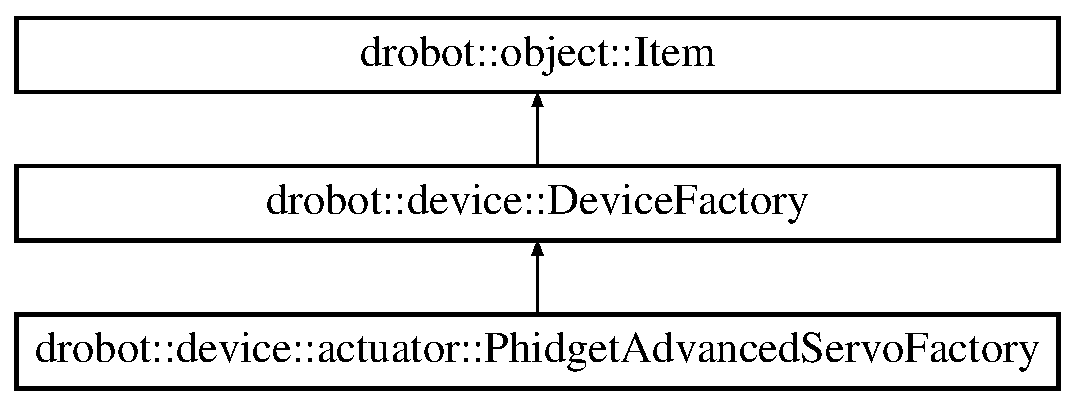
\includegraphics[height=3.000000cm]{classdrobot_1_1device_1_1actuator_1_1PhidgetAdvancedServoFactory}
\end{center}
\end{figure}
\subsection*{Public Member Functions}
\begin{DoxyCompactItemize}
\item 
virtual void \hyperlink{classdrobot_1_1device_1_1actuator_1_1PhidgetAdvancedServoFactory_a05fc8ede82777f4310ac0cf96e705dbe}{create\-From\-Dom\-Element} (Q\-Dom\-Element element, \hyperlink{classdrobot_1_1robot_1_1Robot}{robot\-::\-Robot} $\ast$robot)
\begin{DoxyCompactList}\small\item\em create\-From\-Dom\-Element \end{DoxyCompactList}\end{DoxyCompactItemize}
\subsection*{Additional Inherited Members}


\subsection{Member Function Documentation}
\hypertarget{classdrobot_1_1device_1_1actuator_1_1PhidgetAdvancedServoFactory_a05fc8ede82777f4310ac0cf96e705dbe}{\index{drobot\-::device\-::actuator\-::\-Phidget\-Advanced\-Servo\-Factory@{drobot\-::device\-::actuator\-::\-Phidget\-Advanced\-Servo\-Factory}!create\-From\-Dom\-Element@{create\-From\-Dom\-Element}}
\index{create\-From\-Dom\-Element@{create\-From\-Dom\-Element}!drobot::device::actuator::PhidgetAdvancedServoFactory@{drobot\-::device\-::actuator\-::\-Phidget\-Advanced\-Servo\-Factory}}
\subsubsection[{create\-From\-Dom\-Element}]{\setlength{\rightskip}{0pt plus 5cm}void drobot\-::device\-::actuator\-::\-Phidget\-Advanced\-Servo\-Factory\-::create\-From\-Dom\-Element (
\begin{DoxyParamCaption}
\item[{Q\-Dom\-Element}]{element, }
\item[{{\bf robot\-::\-Robot} $\ast$}]{robot}
\end{DoxyParamCaption}
)\hspace{0.3cm}{\ttfamily [virtual]}}}\label{classdrobot_1_1device_1_1actuator_1_1PhidgetAdvancedServoFactory_a05fc8ede82777f4310ac0cf96e705dbe}


create\-From\-Dom\-Element 


\begin{DoxyParams}{Parameters}
{\em element} & \\
\hline
{\em robot} & \\
\hline
\end{DoxyParams}
Creates a device from a Q\-Dom\-Element. This method should add the device of the robots \hyperlink{classdrobot_1_1device_1_1DeviceManager}{Device\-Manager}. If the created \hyperlink{classdrobot_1_1device_1_1Device}{Device} is a Controller the controller property of the robot should also be set. Each device element may contain channel elements which have to be parsed by the channel\-Factories. Also if the device have need of a \hyperlink{classdrobot_1_1device_1_1DeviceBoard}{Device\-Board} it should be added to the \hyperlink{classdrobot_1_1device_1_1DeviceManager}{Device\-Manager} too. See actuator/phidgetadvancedservofactory.\-cpp for an example. 

Implements \hyperlink{classdrobot_1_1device_1_1DeviceFactory_af9234abdb75d5a0129630baabe0c98cc}{drobot\-::device\-::\-Device\-Factory}.



The documentation for this class was generated from the following files\-:\begin{DoxyCompactItemize}
\item 
/home/imanol/workspace/drobot/new/src/drobot/device/actuator/phidgetadvancedservofactory.\-h\item 
/home/imanol/workspace/drobot/new/src/drobot/device/actuator/phidgetadvancedservofactory.\-cpp\end{DoxyCompactItemize}

\hypertarget{classdrobot_1_1device_1_1PhidgetDevice}{\section{drobot\-:\-:device\-:\-:Phidget\-Device Class Reference}
\label{classdrobot_1_1device_1_1PhidgetDevice}\index{drobot\-::device\-::\-Phidget\-Device@{drobot\-::device\-::\-Phidget\-Device}}
}


Base class for all Phidget Devices. Implements the standard functions.  




{\ttfamily \#include $<$phidgetdevice.\-h$>$}

Inheritance diagram for drobot\-:\-:device\-:\-:Phidget\-Device\-:\begin{figure}[H]
\begin{center}
\leavevmode
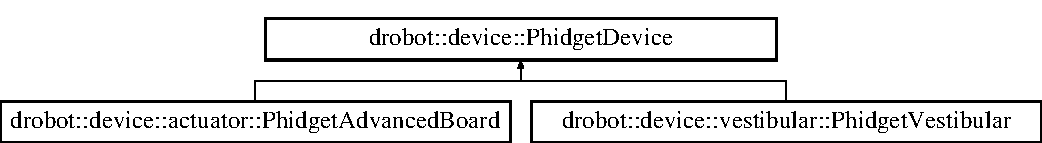
\includegraphics[height=1.917808cm]{classdrobot_1_1device_1_1PhidgetDevice}
\end{center}
\end{figure}
\subsection*{Public Member Functions}
\begin{DoxyCompactItemize}
\item 
\hypertarget{classdrobot_1_1device_1_1PhidgetDevice_ac28787f45dfd3c71b5975468e6367093}{std\-::string {\bfseries get\-Phidget\-Name} ()}\label{classdrobot_1_1device_1_1PhidgetDevice_ac28787f45dfd3c71b5975468e6367093}

\item 
\hypertarget{classdrobot_1_1device_1_1PhidgetDevice_a980d9075de25d1c08c66ef2516edbb1b}{int {\bfseries get\-Phidget\-Serial\-Number} ()}\label{classdrobot_1_1device_1_1PhidgetDevice_a980d9075de25d1c08c66ef2516edbb1b}

\item 
\hypertarget{classdrobot_1_1device_1_1PhidgetDevice_aa743ddee3b9c83810d9099057d36d3dd}{int {\bfseries get\-Phidget\-Version} ()}\label{classdrobot_1_1device_1_1PhidgetDevice_aa743ddee3b9c83810d9099057d36d3dd}

\item 
\hypertarget{classdrobot_1_1device_1_1PhidgetDevice_ab41dcce452b38672d3920d3a10983c2d}{int {\bfseries get\-Phidget\-Status} ()}\label{classdrobot_1_1device_1_1PhidgetDevice_ab41dcce452b38672d3920d3a10983c2d}

\item 
\hypertarget{classdrobot_1_1device_1_1PhidgetDevice_ae96e8f3e5368a5dda19e62d992dedb6e}{std\-::string {\bfseries get\-Phidget\-Type} ()}\label{classdrobot_1_1device_1_1PhidgetDevice_ae96e8f3e5368a5dda19e62d992dedb6e}

\item 
\hypertarget{classdrobot_1_1device_1_1PhidgetDevice_a8ab02715b4634ef696e1f213c3641a4e}{std\-::string {\bfseries get\-Phidget\-Label} ()}\label{classdrobot_1_1device_1_1PhidgetDevice_a8ab02715b4634ef696e1f213c3641a4e}

\item 
\hypertarget{classdrobot_1_1device_1_1PhidgetDevice_a286495c77b06ef134bebdafa39a389de}{void {\bfseries set\-Phidget\-Label} (std\-::string label)}\label{classdrobot_1_1device_1_1PhidgetDevice_a286495c77b06ef134bebdafa39a389de}

\item 
\hypertarget{classdrobot_1_1device_1_1PhidgetDevice_a42bc77706b62ec51a5cbacf9025b87fb}{C\-Phidget\-\_\-\-Device\-I\-D {\bfseries get\-Phidget\-Id} ()}\label{classdrobot_1_1device_1_1PhidgetDevice_a42bc77706b62ec51a5cbacf9025b87fb}

\end{DoxyCompactItemize}
\subsection*{Protected Member Functions}
\begin{DoxyCompactItemize}
\item 
virtual C\-Phidget\-Handle \hyperlink{classdrobot_1_1device_1_1PhidgetDevice_a0bcc3051d4a096d92b428a3166e78861}{get\-Phidget\-Handle} ()=0
\begin{DoxyCompactList}\small\item\em Must be implemented by the specific phidget device to return a C\-Phidget\-Handle struct. \end{DoxyCompactList}\end{DoxyCompactItemize}


\subsection{Detailed Description}
Base class for all Phidget Devices. Implements the standard functions. 

\subsection{Member Function Documentation}
\hypertarget{classdrobot_1_1device_1_1PhidgetDevice_a0bcc3051d4a096d92b428a3166e78861}{\index{drobot\-::device\-::\-Phidget\-Device@{drobot\-::device\-::\-Phidget\-Device}!get\-Phidget\-Handle@{get\-Phidget\-Handle}}
\index{get\-Phidget\-Handle@{get\-Phidget\-Handle}!drobot::device::PhidgetDevice@{drobot\-::device\-::\-Phidget\-Device}}
\subsubsection[{get\-Phidget\-Handle}]{\setlength{\rightskip}{0pt plus 5cm}virtual C\-Phidget\-Handle drobot\-::device\-::\-Phidget\-Device\-::get\-Phidget\-Handle (
\begin{DoxyParamCaption}
{}
\end{DoxyParamCaption}
)\hspace{0.3cm}{\ttfamily [protected]}, {\ttfamily [pure virtual]}}}\label{classdrobot_1_1device_1_1PhidgetDevice_a0bcc3051d4a096d92b428a3166e78861}


Must be implemented by the specific phidget device to return a C\-Phidget\-Handle struct. 

\begin{DoxyReturn}{Returns}

\end{DoxyReturn}


Implemented in \hyperlink{classdrobot_1_1device_1_1actuator_1_1PhidgetAdvancedBoard_a67afbf98c18b80281226259f93fdb742}{drobot\-::device\-::actuator\-::\-Phidget\-Advanced\-Board}, and \hyperlink{classdrobot_1_1device_1_1vestibular_1_1PhidgetVestibular_a8292d6ebbc1910eca84081cf76bf3afe}{drobot\-::device\-::vestibular\-::\-Phidget\-Vestibular}.



The documentation for this class was generated from the following files\-:\begin{DoxyCompactItemize}
\item 
src/drobot/device/phidgetdevice.\-h\item 
src/drobot/device/phidgetdevice.\-cpp\end{DoxyCompactItemize}

\hypertarget{classdrobot_1_1device_1_1actuator_1_1PhidgetSimpleBoard}{\section{drobot\-:\-:device\-:\-:actuator\-:\-:Phidget\-Simple\-Board Class Reference}
\label{classdrobot_1_1device_1_1actuator_1_1PhidgetSimpleBoard}\index{drobot\-::device\-::actuator\-::\-Phidget\-Simple\-Board@{drobot\-::device\-::actuator\-::\-Phidget\-Simple\-Board}}
}


The Phidget Simple Board class.  




{\ttfamily \#include $<$phidgetsimpleboard.\-h$>$}

Inheritance diagram for drobot\-:\-:device\-:\-:actuator\-:\-:Phidget\-Simple\-Board\-:\begin{figure}[H]
\begin{center}
\leavevmode
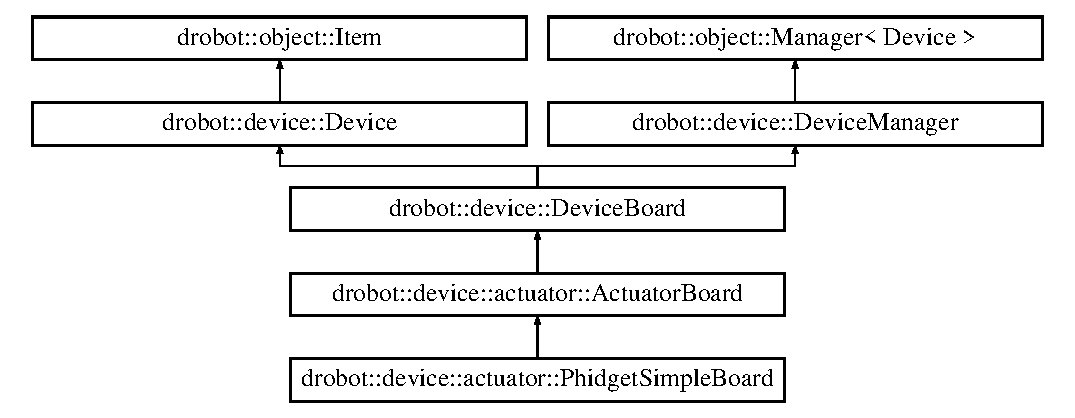
\includegraphics[height=5.000000cm]{classdrobot_1_1device_1_1actuator_1_1PhidgetSimpleBoard}
\end{center}
\end{figure}
\subsection*{Public Member Functions}
\begin{DoxyCompactItemize}
\item 
\hyperlink{classdrobot_1_1device_1_1actuator_1_1PhidgetSimpleBoard_a750faa2124c350c91a114d18e2cc2300}{Phidget\-Simple\-Board} (std\-::string name)
\begin{DoxyCompactList}\small\item\em Initializes a random connected Phidget Simple Board. \end{DoxyCompactList}\item 
\hyperlink{classdrobot_1_1device_1_1actuator_1_1PhidgetSimpleBoard_a24a16a968ecc6e7025b6a0e8089ce694}{Phidget\-Simple\-Board} (std\-::string name, int serial)
\begin{DoxyCompactList}\small\item\em Initializes the Phidget Simple Board with the given serial. \end{DoxyCompactList}\item 
\hyperlink{classdrobot_1_1device_1_1actuator_1_1PhidgetSimpleBoard_a3d30fd69c7dc2030a13e128b020e2ce1}{Phidget\-Simple\-Board} (std\-::string name, C\-Phidget\-Servo\-Handle phidget\-Handle)
\begin{DoxyCompactList}\small\item\em Initializes a Phidget Simple Board by the given C\-Phidget\-Servo\-Handle. \end{DoxyCompactList}\item 
int \hyperlink{classdrobot_1_1device_1_1actuator_1_1PhidgetSimpleBoard_ae7472942d639115a395f0ae95e331c47}{get\-Max\-Actuators} ()
\item 
std\-::vector$<$ \hyperlink{classdrobot_1_1device_1_1actuator_1_1Actuator}{Actuator} $\ast$ $>$ \hyperlink{classdrobot_1_1device_1_1actuator_1_1PhidgetSimpleBoard_a1d13867a272da7219da6892f5564c97c}{init\-All\-Actuators} ()
\begin{DoxyCompactList}\small\item\em initializes all the connected Servo Motors and adds them to the board \end{DoxyCompactList}\item 
\hyperlink{classdrobot_1_1device_1_1actuator_1_1Actuator}{Actuator} $\ast$ \hyperlink{classdrobot_1_1device_1_1actuator_1_1PhidgetSimpleBoard_ac3543031be94ce9a6e245a2a73f704f5}{init\-Actuator} (int index, std\-::string name)
\begin{DoxyCompactList}\small\item\em initializes the servomotor at the given index and adds it to the board \end{DoxyCompactList}\item 
\hyperlink{classdrobot_1_1device_1_1actuator_1_1Actuator}{Actuator} $\ast$ \hyperlink{classdrobot_1_1device_1_1actuator_1_1PhidgetSimpleBoard_a7ffef559394dd7d951e6bb9fd24c3bad}{init\-Actuator} (int index)
\begin{DoxyCompactList}\small\item\em initializes the servomotor at the given index and adds it to the board \end{DoxyCompactList}\end{DoxyCompactItemize}
\subsection*{Protected Member Functions}
\begin{DoxyCompactItemize}
\item 
\hypertarget{classdrobot_1_1device_1_1actuator_1_1PhidgetSimpleBoard_ae8305bb67f96e56805fc5a2dc917210a}{virtual C\-Phidget\-Handle \& {\bfseries get\-Phidget\-Handle} ()}\label{classdrobot_1_1device_1_1actuator_1_1PhidgetSimpleBoard_ae8305bb67f96e56805fc5a2dc917210a}

\end{DoxyCompactItemize}
\subsection*{Private Attributes}
\begin{DoxyCompactItemize}
\item 
\hypertarget{classdrobot_1_1device_1_1actuator_1_1PhidgetSimpleBoard_ac085270f4149d7f33e4992eaae8b7e60}{C\-Phidget\-Servo\-Handle {\bfseries \-\_\-phidget\-Handle}}\label{classdrobot_1_1device_1_1actuator_1_1PhidgetSimpleBoard_ac085270f4149d7f33e4992eaae8b7e60}

\end{DoxyCompactItemize}
\subsection*{Additional Inherited Members}


\subsection{Detailed Description}
The Phidget Simple Board class. 

This Class handles the \char`\"{}\-Phidget Servo\char`\"{} board. The Phidget Simple Board contains Phidget Simple Servo objects which can be initialized and used independently. 

\subsection{Constructor \& Destructor Documentation}
\hypertarget{classdrobot_1_1device_1_1actuator_1_1PhidgetSimpleBoard_a750faa2124c350c91a114d18e2cc2300}{\index{drobot\-::device\-::actuator\-::\-Phidget\-Simple\-Board@{drobot\-::device\-::actuator\-::\-Phidget\-Simple\-Board}!Phidget\-Simple\-Board@{Phidget\-Simple\-Board}}
\index{Phidget\-Simple\-Board@{Phidget\-Simple\-Board}!drobot::device::actuator::PhidgetSimpleBoard@{drobot\-::device\-::actuator\-::\-Phidget\-Simple\-Board}}
\subsubsection[{Phidget\-Simple\-Board}]{\setlength{\rightskip}{0pt plus 5cm}drobot\-::device\-::actuator\-::\-Phidget\-Simple\-Board\-::\-Phidget\-Simple\-Board (
\begin{DoxyParamCaption}
\item[{std\-::string}]{name}
\end{DoxyParamCaption}
)}}\label{classdrobot_1_1device_1_1actuator_1_1PhidgetSimpleBoard_a750faa2124c350c91a114d18e2cc2300}


Initializes a random connected Phidget Simple Board. 


\begin{DoxyParams}{Parameters}
{\em name} & \\
\hline
\end{DoxyParams}
\hypertarget{classdrobot_1_1device_1_1actuator_1_1PhidgetSimpleBoard_a24a16a968ecc6e7025b6a0e8089ce694}{\index{drobot\-::device\-::actuator\-::\-Phidget\-Simple\-Board@{drobot\-::device\-::actuator\-::\-Phidget\-Simple\-Board}!Phidget\-Simple\-Board@{Phidget\-Simple\-Board}}
\index{Phidget\-Simple\-Board@{Phidget\-Simple\-Board}!drobot::device::actuator::PhidgetSimpleBoard@{drobot\-::device\-::actuator\-::\-Phidget\-Simple\-Board}}
\subsubsection[{Phidget\-Simple\-Board}]{\setlength{\rightskip}{0pt plus 5cm}drobot\-::device\-::actuator\-::\-Phidget\-Simple\-Board\-::\-Phidget\-Simple\-Board (
\begin{DoxyParamCaption}
\item[{std\-::string}]{name, }
\item[{int}]{serial}
\end{DoxyParamCaption}
)}}\label{classdrobot_1_1device_1_1actuator_1_1PhidgetSimpleBoard_a24a16a968ecc6e7025b6a0e8089ce694}


Initializes the Phidget Simple Board with the given serial. 


\begin{DoxyParams}{Parameters}
{\em name} & \\
\hline
{\em serial} & \\
\hline
\end{DoxyParams}
\hypertarget{classdrobot_1_1device_1_1actuator_1_1PhidgetSimpleBoard_a3d30fd69c7dc2030a13e128b020e2ce1}{\index{drobot\-::device\-::actuator\-::\-Phidget\-Simple\-Board@{drobot\-::device\-::actuator\-::\-Phidget\-Simple\-Board}!Phidget\-Simple\-Board@{Phidget\-Simple\-Board}}
\index{Phidget\-Simple\-Board@{Phidget\-Simple\-Board}!drobot::device::actuator::PhidgetSimpleBoard@{drobot\-::device\-::actuator\-::\-Phidget\-Simple\-Board}}
\subsubsection[{Phidget\-Simple\-Board}]{\setlength{\rightskip}{0pt plus 5cm}drobot\-::device\-::actuator\-::\-Phidget\-Simple\-Board\-::\-Phidget\-Simple\-Board (
\begin{DoxyParamCaption}
\item[{std\-::string}]{name, }
\item[{C\-Phidget\-Servo\-Handle}]{phidget\-Handle}
\end{DoxyParamCaption}
)}}\label{classdrobot_1_1device_1_1actuator_1_1PhidgetSimpleBoard_a3d30fd69c7dc2030a13e128b020e2ce1}


Initializes a Phidget Simple Board by the given C\-Phidget\-Servo\-Handle. 


\begin{DoxyParams}{Parameters}
{\em name} & \\
\hline
{\em phidget\-Handle} & \\
\hline
\end{DoxyParams}


\subsection{Member Function Documentation}
\hypertarget{classdrobot_1_1device_1_1actuator_1_1PhidgetSimpleBoard_ae7472942d639115a395f0ae95e331c47}{\index{drobot\-::device\-::actuator\-::\-Phidget\-Simple\-Board@{drobot\-::device\-::actuator\-::\-Phidget\-Simple\-Board}!get\-Max\-Actuators@{get\-Max\-Actuators}}
\index{get\-Max\-Actuators@{get\-Max\-Actuators}!drobot::device::actuator::PhidgetSimpleBoard@{drobot\-::device\-::actuator\-::\-Phidget\-Simple\-Board}}
\subsubsection[{get\-Max\-Actuators}]{\setlength{\rightskip}{0pt plus 5cm}int drobot\-::device\-::actuator\-::\-Phidget\-Simple\-Board\-::get\-Max\-Actuators (
\begin{DoxyParamCaption}
{}
\end{DoxyParamCaption}
)}}\label{classdrobot_1_1device_1_1actuator_1_1PhidgetSimpleBoard_ae7472942d639115a395f0ae95e331c47}
\begin{DoxyReturn}{Returns}
max number of actuators 
\end{DoxyReturn}
\hypertarget{classdrobot_1_1device_1_1actuator_1_1PhidgetSimpleBoard_ac3543031be94ce9a6e245a2a73f704f5}{\index{drobot\-::device\-::actuator\-::\-Phidget\-Simple\-Board@{drobot\-::device\-::actuator\-::\-Phidget\-Simple\-Board}!init\-Actuator@{init\-Actuator}}
\index{init\-Actuator@{init\-Actuator}!drobot::device::actuator::PhidgetSimpleBoard@{drobot\-::device\-::actuator\-::\-Phidget\-Simple\-Board}}
\subsubsection[{init\-Actuator}]{\setlength{\rightskip}{0pt plus 5cm}{\bf Actuator} $\ast$ drobot\-::device\-::actuator\-::\-Phidget\-Simple\-Board\-::init\-Actuator (
\begin{DoxyParamCaption}
\item[{int}]{index, }
\item[{std\-::string}]{name}
\end{DoxyParamCaption}
)}}\label{classdrobot_1_1device_1_1actuator_1_1PhidgetSimpleBoard_ac3543031be94ce9a6e245a2a73f704f5}


initializes the servomotor at the given index and adds it to the board 


\begin{DoxyParams}{Parameters}
{\em index} & \\
\hline
{\em name} & of the servomotor \\
\hline
\end{DoxyParams}
\begin{DoxyReturn}{Returns}
the initialized servomotor 
\end{DoxyReturn}
\hypertarget{classdrobot_1_1device_1_1actuator_1_1PhidgetSimpleBoard_a7ffef559394dd7d951e6bb9fd24c3bad}{\index{drobot\-::device\-::actuator\-::\-Phidget\-Simple\-Board@{drobot\-::device\-::actuator\-::\-Phidget\-Simple\-Board}!init\-Actuator@{init\-Actuator}}
\index{init\-Actuator@{init\-Actuator}!drobot::device::actuator::PhidgetSimpleBoard@{drobot\-::device\-::actuator\-::\-Phidget\-Simple\-Board}}
\subsubsection[{init\-Actuator}]{\setlength{\rightskip}{0pt plus 5cm}{\bf Actuator} $\ast$ drobot\-::device\-::actuator\-::\-Phidget\-Simple\-Board\-::init\-Actuator (
\begin{DoxyParamCaption}
\item[{int}]{index}
\end{DoxyParamCaption}
)}}\label{classdrobot_1_1device_1_1actuator_1_1PhidgetSimpleBoard_a7ffef559394dd7d951e6bb9fd24c3bad}


initializes the servomotor at the given index and adds it to the board 


\begin{DoxyParams}{Parameters}
{\em index} & \\
\hline
\end{DoxyParams}
\begin{DoxyReturn}{Returns}
the initialized servomotor 
\end{DoxyReturn}
\hypertarget{classdrobot_1_1device_1_1actuator_1_1PhidgetSimpleBoard_a1d13867a272da7219da6892f5564c97c}{\index{drobot\-::device\-::actuator\-::\-Phidget\-Simple\-Board@{drobot\-::device\-::actuator\-::\-Phidget\-Simple\-Board}!init\-All\-Actuators@{init\-All\-Actuators}}
\index{init\-All\-Actuators@{init\-All\-Actuators}!drobot::device::actuator::PhidgetSimpleBoard@{drobot\-::device\-::actuator\-::\-Phidget\-Simple\-Board}}
\subsubsection[{init\-All\-Actuators}]{\setlength{\rightskip}{0pt plus 5cm}std\-::vector$<$ {\bf Actuator} $\ast$ $>$ drobot\-::device\-::actuator\-::\-Phidget\-Simple\-Board\-::init\-All\-Actuators (
\begin{DoxyParamCaption}
{}
\end{DoxyParamCaption}
)}}\label{classdrobot_1_1device_1_1actuator_1_1PhidgetSimpleBoard_a1d13867a272da7219da6892f5564c97c}


initializes all the connected Servo Motors and adds them to the board 

\begin{DoxyReturn}{Returns}
initialized servos 
\end{DoxyReturn}


The documentation for this class was generated from the following files\-:\begin{DoxyCompactItemize}
\item 
/home/imanol/workspace/drobot/new/src/drobot/device/actuator/phidgetsimpleboard.\-h\item 
/home/imanol/workspace/drobot/new/src/drobot/device/actuator/phidgetsimpleboard.\-cpp\end{DoxyCompactItemize}

\hypertarget{classdrobot_1_1device_1_1actuator_1_1PhidgetSimpleServo}{\section{drobot\-:\-:device\-:\-:actuator\-:\-:Phidget\-Simple\-Servo Class Reference}
\label{classdrobot_1_1device_1_1actuator_1_1PhidgetSimpleServo}\index{drobot\-::device\-::actuator\-::\-Phidget\-Simple\-Servo@{drobot\-::device\-::actuator\-::\-Phidget\-Simple\-Servo}}
}


The \hyperlink{classdrobot_1_1device_1_1actuator_1_1PhidgetSimpleServo}{Phidget\-Simple\-Servo} class.  




{\ttfamily \#include $<$phidgetsimpleservo.\-h$>$}

Inheritance diagram for drobot\-:\-:device\-:\-:actuator\-:\-:Phidget\-Simple\-Servo\-:\begin{figure}[H]
\begin{center}
\leavevmode
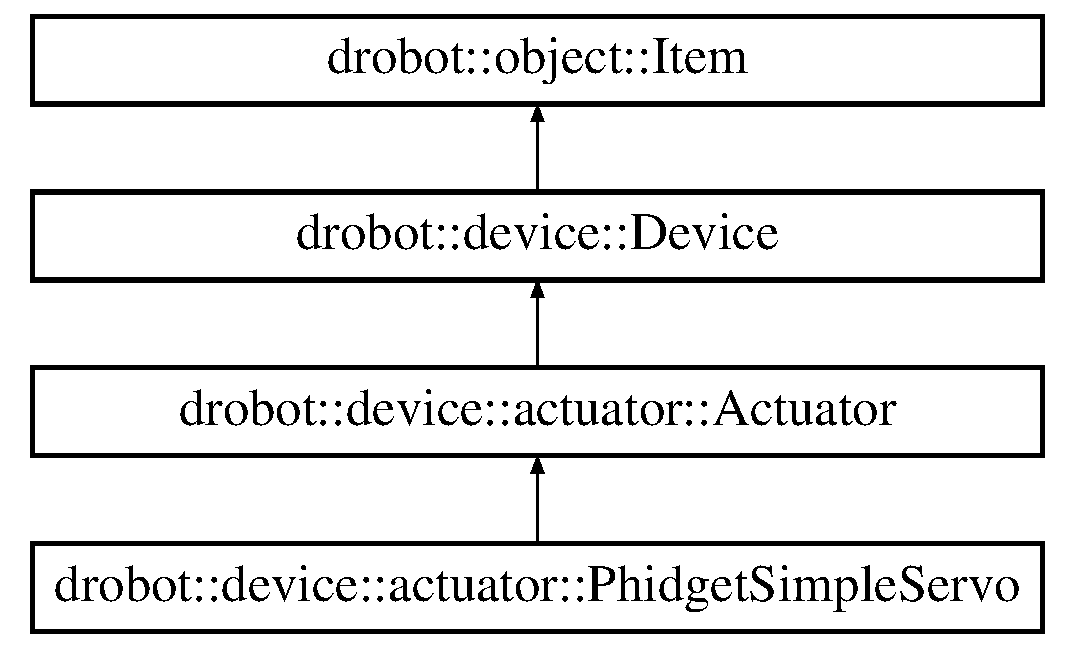
\includegraphics[height=4.000000cm]{classdrobot_1_1device_1_1actuator_1_1PhidgetSimpleServo}
\end{center}
\end{figure}
\subsection*{Public Member Functions}
\begin{DoxyCompactItemize}
\item 
\hypertarget{classdrobot_1_1device_1_1actuator_1_1PhidgetSimpleServo_aa9a6d23acae8bb34343ba9c1bd7cc9a1}{{\bfseries Phidget\-Simple\-Servo} (std\-::string name, C\-Phidget\-Servo\-Handle phidget\-Handle, int index)}\label{classdrobot_1_1device_1_1actuator_1_1PhidgetSimpleServo_aa9a6d23acae8bb34343ba9c1bd7cc9a1}

\item 
virtual void \hyperlink{classdrobot_1_1device_1_1actuator_1_1PhidgetSimpleServo_ada2b985fee1f6a3891effad83fb7f738}{enable} ()
\begin{DoxyCompactList}\small\item\em enables the device. \end{DoxyCompactList}\item 
virtual void \hyperlink{classdrobot_1_1device_1_1actuator_1_1PhidgetSimpleServo_ad3dffbddc718a4f447a75bc90c0cb8f1}{disable} ()
\begin{DoxyCompactList}\small\item\em disables the device. \end{DoxyCompactList}\item 
virtual bool \hyperlink{classdrobot_1_1device_1_1actuator_1_1PhidgetSimpleServo_a6da8b37b613ecf9c8fc12f335ec90537}{is\-Enabled} ()
\begin{DoxyCompactList}\small\item\em check if the device is enabled \end{DoxyCompactList}\item 
virtual double \hyperlink{classdrobot_1_1device_1_1actuator_1_1PhidgetSimpleServo_a4b63fb0ed00c9594037a53827b3bfdb5}{get\-Position} ()
\item 
virtual void \hyperlink{classdrobot_1_1device_1_1actuator_1_1PhidgetSimpleServo_a9c08fb8a75bded49f53635d9184ce9e2}{set\-Position} (double position)
\begin{DoxyCompactList}\small\item\em set motor position. The motor will always move to the last set position. \end{DoxyCompactList}\item 
virtual double \hyperlink{classdrobot_1_1device_1_1actuator_1_1PhidgetSimpleServo_a37cbebc54653841ec66e3176a3e46241}{get\-Position\-Min} ()
\item 
virtual double \hyperlink{classdrobot_1_1device_1_1actuator_1_1PhidgetSimpleServo_a6a0c6bc3edd91bc7cdcbb3ceb6e35499}{get\-Position\-Max} ()
\item 
virtual double \hyperlink{classdrobot_1_1device_1_1actuator_1_1PhidgetSimpleServo_ac95f8be440b0fbed1c9d33b2d919d804}{get\-Velocity} ()
\item 
virtual void \hyperlink{classdrobot_1_1device_1_1actuator_1_1PhidgetSimpleServo_af0c80a2d8cacc535b7b529eb84fc1075}{set\-Velocity} (double velocity)
\begin{DoxyCompactList}\small\item\em set current velocity \end{DoxyCompactList}\item 
virtual double \hyperlink{classdrobot_1_1device_1_1actuator_1_1PhidgetSimpleServo_a9880f9f9f0cd83abc3b8d927316ed843}{get\-Velocity\-Min} ()
\item 
virtual double \hyperlink{classdrobot_1_1device_1_1actuator_1_1PhidgetSimpleServo_aa54b52796cfb651db75b762dc319b38f}{get\-Velocity\-Max} ()
\item 
virtual double \hyperlink{classdrobot_1_1device_1_1actuator_1_1PhidgetSimpleServo_ab9aee84e3e9b714298df2891f9bf9d89}{get\-Acceleration} ()
\item 
virtual void \hyperlink{classdrobot_1_1device_1_1actuator_1_1PhidgetSimpleServo_a9577403e844e3d18f66fd23c2bdf1e8f}{set\-Acceleration} (double acceleration)
\begin{DoxyCompactList}\small\item\em set current acceleration \end{DoxyCompactList}\item 
virtual double \hyperlink{classdrobot_1_1device_1_1actuator_1_1PhidgetSimpleServo_a76961c60cfa11ddae2588555eba8a223}{get\-Acceleration\-Min} ()
\item 
virtual double \hyperlink{classdrobot_1_1device_1_1actuator_1_1PhidgetSimpleServo_a33019d0481fe3e18179291c3090bb8aa}{get\-Acceleration\-Max} ()
\end{DoxyCompactItemize}
\subsection*{Protected Member Functions}
\begin{DoxyCompactItemize}
\item 
\hypertarget{classdrobot_1_1device_1_1actuator_1_1PhidgetSimpleServo_a7651960d50dda3b1e2b4133f25b0da03}{virtual C\-Phidget\-Handle \& {\bfseries get\-Phidget\-Handle} ()}\label{classdrobot_1_1device_1_1actuator_1_1PhidgetSimpleServo_a7651960d50dda3b1e2b4133f25b0da03}

\end{DoxyCompactItemize}
\subsection*{Private Attributes}
\begin{DoxyCompactItemize}
\item 
\hypertarget{classdrobot_1_1device_1_1actuator_1_1PhidgetSimpleServo_ae79da953241949d3ab10a86045551b80}{C\-Phidget\-Servo\-Handle {\bfseries \-\_\-phidget\-Handle}}\label{classdrobot_1_1device_1_1actuator_1_1PhidgetSimpleServo_ae79da953241949d3ab10a86045551b80}

\item 
\hypertarget{classdrobot_1_1device_1_1actuator_1_1PhidgetSimpleServo_a69447db2b624fd79316f9570aa67aab8}{int {\bfseries \-\_\-index}}\label{classdrobot_1_1device_1_1actuator_1_1PhidgetSimpleServo_a69447db2b624fd79316f9570aa67aab8}

\end{DoxyCompactItemize}
\subsection*{Additional Inherited Members}


\subsection{Detailed Description}
The \hyperlink{classdrobot_1_1device_1_1actuator_1_1PhidgetSimpleServo}{Phidget\-Simple\-Servo} class. 

The \hyperlink{classdrobot_1_1device_1_1actuator_1_1PhidgetSimpleServo}{Phidget\-Simple\-Servo} only supports movement by setting the position. The acceleration and velocity properties aren't implemented by the Phidget Servo module but they can be simulated by setting the position according to the acceleration/velocity set if needed. 

\subsection{Member Function Documentation}
\hypertarget{classdrobot_1_1device_1_1actuator_1_1PhidgetSimpleServo_ad3dffbddc718a4f447a75bc90c0cb8f1}{\index{drobot\-::device\-::actuator\-::\-Phidget\-Simple\-Servo@{drobot\-::device\-::actuator\-::\-Phidget\-Simple\-Servo}!disable@{disable}}
\index{disable@{disable}!drobot::device::actuator::PhidgetSimpleServo@{drobot\-::device\-::actuator\-::\-Phidget\-Simple\-Servo}}
\subsubsection[{disable}]{\setlength{\rightskip}{0pt plus 5cm}void drobot\-::device\-::actuator\-::\-Phidget\-Simple\-Servo\-::disable (
\begin{DoxyParamCaption}
{}
\end{DoxyParamCaption}
)\hspace{0.3cm}{\ttfamily [virtual]}}}\label{classdrobot_1_1device_1_1actuator_1_1PhidgetSimpleServo_ad3dffbddc718a4f447a75bc90c0cb8f1}


disables the device. 

This function has to be implemented by the specific device. For physical devices like actuators this method should power off the device; 

Reimplemented from \hyperlink{classdrobot_1_1device_1_1Device_a289499673ae30bd72101c68fbd04cd89}{drobot\-::device\-::\-Device}.

\hypertarget{classdrobot_1_1device_1_1actuator_1_1PhidgetSimpleServo_ada2b985fee1f6a3891effad83fb7f738}{\index{drobot\-::device\-::actuator\-::\-Phidget\-Simple\-Servo@{drobot\-::device\-::actuator\-::\-Phidget\-Simple\-Servo}!enable@{enable}}
\index{enable@{enable}!drobot::device::actuator::PhidgetSimpleServo@{drobot\-::device\-::actuator\-::\-Phidget\-Simple\-Servo}}
\subsubsection[{enable}]{\setlength{\rightskip}{0pt plus 5cm}void drobot\-::device\-::actuator\-::\-Phidget\-Simple\-Servo\-::enable (
\begin{DoxyParamCaption}
{}
\end{DoxyParamCaption}
)\hspace{0.3cm}{\ttfamily [virtual]}}}\label{classdrobot_1_1device_1_1actuator_1_1PhidgetSimpleServo_ada2b985fee1f6a3891effad83fb7f738}


enables the device. 

This function has to be implemented by the specific device. For physical devices like actuators this method should power on the device. 

Reimplemented from \hyperlink{classdrobot_1_1device_1_1Device_a0c28785ff2e79f99b8e9eaefe6749f2b}{drobot\-::device\-::\-Device}.

\hypertarget{classdrobot_1_1device_1_1actuator_1_1PhidgetSimpleServo_ab9aee84e3e9b714298df2891f9bf9d89}{\index{drobot\-::device\-::actuator\-::\-Phidget\-Simple\-Servo@{drobot\-::device\-::actuator\-::\-Phidget\-Simple\-Servo}!get\-Acceleration@{get\-Acceleration}}
\index{get\-Acceleration@{get\-Acceleration}!drobot::device::actuator::PhidgetSimpleServo@{drobot\-::device\-::actuator\-::\-Phidget\-Simple\-Servo}}
\subsubsection[{get\-Acceleration}]{\setlength{\rightskip}{0pt plus 5cm}double drobot\-::device\-::actuator\-::\-Phidget\-Simple\-Servo\-::get\-Acceleration (
\begin{DoxyParamCaption}
{}
\end{DoxyParamCaption}
)\hspace{0.3cm}{\ttfamily [virtual]}}}\label{classdrobot_1_1device_1_1actuator_1_1PhidgetSimpleServo_ab9aee84e3e9b714298df2891f9bf9d89}
\begin{DoxyReturn}{Returns}
current acceleration 
\end{DoxyReturn}


Implements \hyperlink{classdrobot_1_1device_1_1actuator_1_1Actuator_a9dd6e74032417e5a84946925c655047c}{drobot\-::device\-::actuator\-::\-Actuator}.

\hypertarget{classdrobot_1_1device_1_1actuator_1_1PhidgetSimpleServo_a33019d0481fe3e18179291c3090bb8aa}{\index{drobot\-::device\-::actuator\-::\-Phidget\-Simple\-Servo@{drobot\-::device\-::actuator\-::\-Phidget\-Simple\-Servo}!get\-Acceleration\-Max@{get\-Acceleration\-Max}}
\index{get\-Acceleration\-Max@{get\-Acceleration\-Max}!drobot::device::actuator::PhidgetSimpleServo@{drobot\-::device\-::actuator\-::\-Phidget\-Simple\-Servo}}
\subsubsection[{get\-Acceleration\-Max}]{\setlength{\rightskip}{0pt plus 5cm}double drobot\-::device\-::actuator\-::\-Phidget\-Simple\-Servo\-::get\-Acceleration\-Max (
\begin{DoxyParamCaption}
{}
\end{DoxyParamCaption}
)\hspace{0.3cm}{\ttfamily [virtual]}}}\label{classdrobot_1_1device_1_1actuator_1_1PhidgetSimpleServo_a33019d0481fe3e18179291c3090bb8aa}
\begin{DoxyReturn}{Returns}
maximal possible acceleration 
\end{DoxyReturn}


Implements \hyperlink{classdrobot_1_1device_1_1actuator_1_1Actuator_a74e4fc92b8a3661ccbc44435411fbfca}{drobot\-::device\-::actuator\-::\-Actuator}.

\hypertarget{classdrobot_1_1device_1_1actuator_1_1PhidgetSimpleServo_a76961c60cfa11ddae2588555eba8a223}{\index{drobot\-::device\-::actuator\-::\-Phidget\-Simple\-Servo@{drobot\-::device\-::actuator\-::\-Phidget\-Simple\-Servo}!get\-Acceleration\-Min@{get\-Acceleration\-Min}}
\index{get\-Acceleration\-Min@{get\-Acceleration\-Min}!drobot::device::actuator::PhidgetSimpleServo@{drobot\-::device\-::actuator\-::\-Phidget\-Simple\-Servo}}
\subsubsection[{get\-Acceleration\-Min}]{\setlength{\rightskip}{0pt plus 5cm}double drobot\-::device\-::actuator\-::\-Phidget\-Simple\-Servo\-::get\-Acceleration\-Min (
\begin{DoxyParamCaption}
{}
\end{DoxyParamCaption}
)\hspace{0.3cm}{\ttfamily [virtual]}}}\label{classdrobot_1_1device_1_1actuator_1_1PhidgetSimpleServo_a76961c60cfa11ddae2588555eba8a223}
\begin{DoxyReturn}{Returns}
minimal possible acceleration 
\end{DoxyReturn}


Implements \hyperlink{classdrobot_1_1device_1_1actuator_1_1Actuator_a16714b00aafdd84affaf9bc3a8383c48}{drobot\-::device\-::actuator\-::\-Actuator}.

\hypertarget{classdrobot_1_1device_1_1actuator_1_1PhidgetSimpleServo_a4b63fb0ed00c9594037a53827b3bfdb5}{\index{drobot\-::device\-::actuator\-::\-Phidget\-Simple\-Servo@{drobot\-::device\-::actuator\-::\-Phidget\-Simple\-Servo}!get\-Position@{get\-Position}}
\index{get\-Position@{get\-Position}!drobot::device::actuator::PhidgetSimpleServo@{drobot\-::device\-::actuator\-::\-Phidget\-Simple\-Servo}}
\subsubsection[{get\-Position}]{\setlength{\rightskip}{0pt plus 5cm}double drobot\-::device\-::actuator\-::\-Phidget\-Simple\-Servo\-::get\-Position (
\begin{DoxyParamCaption}
{}
\end{DoxyParamCaption}
)\hspace{0.3cm}{\ttfamily [virtual]}}}\label{classdrobot_1_1device_1_1actuator_1_1PhidgetSimpleServo_a4b63fb0ed00c9594037a53827b3bfdb5}
\begin{DoxyReturn}{Returns}
current motor position 
\end{DoxyReturn}


Implements \hyperlink{classdrobot_1_1device_1_1actuator_1_1Actuator_aea525e325f2eb2058a37db3e014bb872}{drobot\-::device\-::actuator\-::\-Actuator}.

\hypertarget{classdrobot_1_1device_1_1actuator_1_1PhidgetSimpleServo_a6a0c6bc3edd91bc7cdcbb3ceb6e35499}{\index{drobot\-::device\-::actuator\-::\-Phidget\-Simple\-Servo@{drobot\-::device\-::actuator\-::\-Phidget\-Simple\-Servo}!get\-Position\-Max@{get\-Position\-Max}}
\index{get\-Position\-Max@{get\-Position\-Max}!drobot::device::actuator::PhidgetSimpleServo@{drobot\-::device\-::actuator\-::\-Phidget\-Simple\-Servo}}
\subsubsection[{get\-Position\-Max}]{\setlength{\rightskip}{0pt plus 5cm}double drobot\-::device\-::actuator\-::\-Phidget\-Simple\-Servo\-::get\-Position\-Max (
\begin{DoxyParamCaption}
{}
\end{DoxyParamCaption}
)\hspace{0.3cm}{\ttfamily [virtual]}}}\label{classdrobot_1_1device_1_1actuator_1_1PhidgetSimpleServo_a6a0c6bc3edd91bc7cdcbb3ceb6e35499}
\begin{DoxyReturn}{Returns}
minimal possible position 
\end{DoxyReturn}


Implements \hyperlink{classdrobot_1_1device_1_1actuator_1_1Actuator_a3a02ed0a72f8ab360748df0d9872eeb3}{drobot\-::device\-::actuator\-::\-Actuator}.

\hypertarget{classdrobot_1_1device_1_1actuator_1_1PhidgetSimpleServo_a37cbebc54653841ec66e3176a3e46241}{\index{drobot\-::device\-::actuator\-::\-Phidget\-Simple\-Servo@{drobot\-::device\-::actuator\-::\-Phidget\-Simple\-Servo}!get\-Position\-Min@{get\-Position\-Min}}
\index{get\-Position\-Min@{get\-Position\-Min}!drobot::device::actuator::PhidgetSimpleServo@{drobot\-::device\-::actuator\-::\-Phidget\-Simple\-Servo}}
\subsubsection[{get\-Position\-Min}]{\setlength{\rightskip}{0pt plus 5cm}double drobot\-::device\-::actuator\-::\-Phidget\-Simple\-Servo\-::get\-Position\-Min (
\begin{DoxyParamCaption}
{}
\end{DoxyParamCaption}
)\hspace{0.3cm}{\ttfamily [virtual]}}}\label{classdrobot_1_1device_1_1actuator_1_1PhidgetSimpleServo_a37cbebc54653841ec66e3176a3e46241}
\begin{DoxyReturn}{Returns}
maximal possible position 
\end{DoxyReturn}


Implements \hyperlink{classdrobot_1_1device_1_1actuator_1_1Actuator_a7a4c195442470d46275f62446e5d2535}{drobot\-::device\-::actuator\-::\-Actuator}.

\hypertarget{classdrobot_1_1device_1_1actuator_1_1PhidgetSimpleServo_ac95f8be440b0fbed1c9d33b2d919d804}{\index{drobot\-::device\-::actuator\-::\-Phidget\-Simple\-Servo@{drobot\-::device\-::actuator\-::\-Phidget\-Simple\-Servo}!get\-Velocity@{get\-Velocity}}
\index{get\-Velocity@{get\-Velocity}!drobot::device::actuator::PhidgetSimpleServo@{drobot\-::device\-::actuator\-::\-Phidget\-Simple\-Servo}}
\subsubsection[{get\-Velocity}]{\setlength{\rightskip}{0pt plus 5cm}double drobot\-::device\-::actuator\-::\-Phidget\-Simple\-Servo\-::get\-Velocity (
\begin{DoxyParamCaption}
{}
\end{DoxyParamCaption}
)\hspace{0.3cm}{\ttfamily [virtual]}}}\label{classdrobot_1_1device_1_1actuator_1_1PhidgetSimpleServo_ac95f8be440b0fbed1c9d33b2d919d804}
\begin{DoxyReturn}{Returns}
current velocity 
\end{DoxyReturn}


Implements \hyperlink{classdrobot_1_1device_1_1actuator_1_1Actuator_a9fea4e618e465cbcc9a207740dbc5410}{drobot\-::device\-::actuator\-::\-Actuator}.

\hypertarget{classdrobot_1_1device_1_1actuator_1_1PhidgetSimpleServo_aa54b52796cfb651db75b762dc319b38f}{\index{drobot\-::device\-::actuator\-::\-Phidget\-Simple\-Servo@{drobot\-::device\-::actuator\-::\-Phidget\-Simple\-Servo}!get\-Velocity\-Max@{get\-Velocity\-Max}}
\index{get\-Velocity\-Max@{get\-Velocity\-Max}!drobot::device::actuator::PhidgetSimpleServo@{drobot\-::device\-::actuator\-::\-Phidget\-Simple\-Servo}}
\subsubsection[{get\-Velocity\-Max}]{\setlength{\rightskip}{0pt plus 5cm}double drobot\-::device\-::actuator\-::\-Phidget\-Simple\-Servo\-::get\-Velocity\-Max (
\begin{DoxyParamCaption}
{}
\end{DoxyParamCaption}
)\hspace{0.3cm}{\ttfamily [virtual]}}}\label{classdrobot_1_1device_1_1actuator_1_1PhidgetSimpleServo_aa54b52796cfb651db75b762dc319b38f}
\begin{DoxyReturn}{Returns}
maximal possible velocity 
\end{DoxyReturn}


Implements \hyperlink{classdrobot_1_1device_1_1actuator_1_1Actuator_a5a018f4e240fb1a483307c03a7662f3d}{drobot\-::device\-::actuator\-::\-Actuator}.

\hypertarget{classdrobot_1_1device_1_1actuator_1_1PhidgetSimpleServo_a9880f9f9f0cd83abc3b8d927316ed843}{\index{drobot\-::device\-::actuator\-::\-Phidget\-Simple\-Servo@{drobot\-::device\-::actuator\-::\-Phidget\-Simple\-Servo}!get\-Velocity\-Min@{get\-Velocity\-Min}}
\index{get\-Velocity\-Min@{get\-Velocity\-Min}!drobot::device::actuator::PhidgetSimpleServo@{drobot\-::device\-::actuator\-::\-Phidget\-Simple\-Servo}}
\subsubsection[{get\-Velocity\-Min}]{\setlength{\rightskip}{0pt plus 5cm}double drobot\-::device\-::actuator\-::\-Phidget\-Simple\-Servo\-::get\-Velocity\-Min (
\begin{DoxyParamCaption}
{}
\end{DoxyParamCaption}
)\hspace{0.3cm}{\ttfamily [virtual]}}}\label{classdrobot_1_1device_1_1actuator_1_1PhidgetSimpleServo_a9880f9f9f0cd83abc3b8d927316ed843}
\begin{DoxyReturn}{Returns}
minimal possible velocity 
\end{DoxyReturn}


Implements \hyperlink{classdrobot_1_1device_1_1actuator_1_1Actuator_a3ddbc25d10ca91b0719ad8b3b6220948}{drobot\-::device\-::actuator\-::\-Actuator}.

\hypertarget{classdrobot_1_1device_1_1actuator_1_1PhidgetSimpleServo_a6da8b37b613ecf9c8fc12f335ec90537}{\index{drobot\-::device\-::actuator\-::\-Phidget\-Simple\-Servo@{drobot\-::device\-::actuator\-::\-Phidget\-Simple\-Servo}!is\-Enabled@{is\-Enabled}}
\index{is\-Enabled@{is\-Enabled}!drobot::device::actuator::PhidgetSimpleServo@{drobot\-::device\-::actuator\-::\-Phidget\-Simple\-Servo}}
\subsubsection[{is\-Enabled}]{\setlength{\rightskip}{0pt plus 5cm}bool drobot\-::device\-::actuator\-::\-Phidget\-Simple\-Servo\-::is\-Enabled (
\begin{DoxyParamCaption}
{}
\end{DoxyParamCaption}
)\hspace{0.3cm}{\ttfamily [virtual]}}}\label{classdrobot_1_1device_1_1actuator_1_1PhidgetSimpleServo_a6da8b37b613ecf9c8fc12f335ec90537}


check if the device is enabled 

\begin{DoxyReturn}{Returns}
true if enabled else false
\end{DoxyReturn}
While the \hyperlink{classdrobot_1_1robot_1_1Robot}{drobot\-::robot\-::\-Robot} is running this property is checked to see whether the device should be used or not. 

Implements \hyperlink{classdrobot_1_1device_1_1Device_aa5b7eac8638d0d2d5ee9bf10607b100e}{drobot\-::device\-::\-Device}.

\hypertarget{classdrobot_1_1device_1_1actuator_1_1PhidgetSimpleServo_a9577403e844e3d18f66fd23c2bdf1e8f}{\index{drobot\-::device\-::actuator\-::\-Phidget\-Simple\-Servo@{drobot\-::device\-::actuator\-::\-Phidget\-Simple\-Servo}!set\-Acceleration@{set\-Acceleration}}
\index{set\-Acceleration@{set\-Acceleration}!drobot::device::actuator::PhidgetSimpleServo@{drobot\-::device\-::actuator\-::\-Phidget\-Simple\-Servo}}
\subsubsection[{set\-Acceleration}]{\setlength{\rightskip}{0pt plus 5cm}void drobot\-::device\-::actuator\-::\-Phidget\-Simple\-Servo\-::set\-Acceleration (
\begin{DoxyParamCaption}
\item[{double}]{acceleration}
\end{DoxyParamCaption}
)\hspace{0.3cm}{\ttfamily [virtual]}}}\label{classdrobot_1_1device_1_1actuator_1_1PhidgetSimpleServo_a9577403e844e3d18f66fd23c2bdf1e8f}


set current acceleration 


\begin{DoxyParams}{Parameters}
{\em acceleration} & \\
\hline
\end{DoxyParams}


Implements \hyperlink{classdrobot_1_1device_1_1actuator_1_1Actuator_a4056ed7c5038c86cd1ed24425a8e2d87}{drobot\-::device\-::actuator\-::\-Actuator}.

\hypertarget{classdrobot_1_1device_1_1actuator_1_1PhidgetSimpleServo_a9c08fb8a75bded49f53635d9184ce9e2}{\index{drobot\-::device\-::actuator\-::\-Phidget\-Simple\-Servo@{drobot\-::device\-::actuator\-::\-Phidget\-Simple\-Servo}!set\-Position@{set\-Position}}
\index{set\-Position@{set\-Position}!drobot::device::actuator::PhidgetSimpleServo@{drobot\-::device\-::actuator\-::\-Phidget\-Simple\-Servo}}
\subsubsection[{set\-Position}]{\setlength{\rightskip}{0pt plus 5cm}void drobot\-::device\-::actuator\-::\-Phidget\-Simple\-Servo\-::set\-Position (
\begin{DoxyParamCaption}
\item[{double}]{position}
\end{DoxyParamCaption}
)\hspace{0.3cm}{\ttfamily [virtual]}}}\label{classdrobot_1_1device_1_1actuator_1_1PhidgetSimpleServo_a9c08fb8a75bded49f53635d9184ce9e2}


set motor position. The motor will always move to the last set position. 


\begin{DoxyParams}{Parameters}
{\em position} & \\
\hline
\end{DoxyParams}


Implements \hyperlink{classdrobot_1_1device_1_1actuator_1_1Actuator_a65fa025b3c0c69d81012454145c7ac69}{drobot\-::device\-::actuator\-::\-Actuator}.

\hypertarget{classdrobot_1_1device_1_1actuator_1_1PhidgetSimpleServo_af0c80a2d8cacc535b7b529eb84fc1075}{\index{drobot\-::device\-::actuator\-::\-Phidget\-Simple\-Servo@{drobot\-::device\-::actuator\-::\-Phidget\-Simple\-Servo}!set\-Velocity@{set\-Velocity}}
\index{set\-Velocity@{set\-Velocity}!drobot::device::actuator::PhidgetSimpleServo@{drobot\-::device\-::actuator\-::\-Phidget\-Simple\-Servo}}
\subsubsection[{set\-Velocity}]{\setlength{\rightskip}{0pt plus 5cm}void drobot\-::device\-::actuator\-::\-Phidget\-Simple\-Servo\-::set\-Velocity (
\begin{DoxyParamCaption}
\item[{double}]{velocity}
\end{DoxyParamCaption}
)\hspace{0.3cm}{\ttfamily [virtual]}}}\label{classdrobot_1_1device_1_1actuator_1_1PhidgetSimpleServo_af0c80a2d8cacc535b7b529eb84fc1075}


set current velocity 


\begin{DoxyParams}{Parameters}
{\em velocity} & \\
\hline
\end{DoxyParams}


Implements \hyperlink{classdrobot_1_1device_1_1actuator_1_1Actuator_a452a63a9cf5daf479c12b99c3e99679c}{drobot\-::device\-::actuator\-::\-Actuator}.



The documentation for this class was generated from the following files\-:\begin{DoxyCompactItemize}
\item 
src/drobot/device/actuator/phidgetsimpleservo.\-h\item 
src/drobot/device/actuator/phidgetsimpleservo.\-cpp\end{DoxyCompactItemize}

\hypertarget{classdrobot_1_1device_1_1actuator_1_1PhidgetSimpleServoFactory}{\section{drobot\-:\-:device\-:\-:actuator\-:\-:Phidget\-Simple\-Servo\-Factory Class Reference}
\label{classdrobot_1_1device_1_1actuator_1_1PhidgetSimpleServoFactory}\index{drobot\-::device\-::actuator\-::\-Phidget\-Simple\-Servo\-Factory@{drobot\-::device\-::actuator\-::\-Phidget\-Simple\-Servo\-Factory}}
}
Inheritance diagram for drobot\-:\-:device\-:\-:actuator\-:\-:Phidget\-Simple\-Servo\-Factory\-:\begin{figure}[H]
\begin{center}
\leavevmode
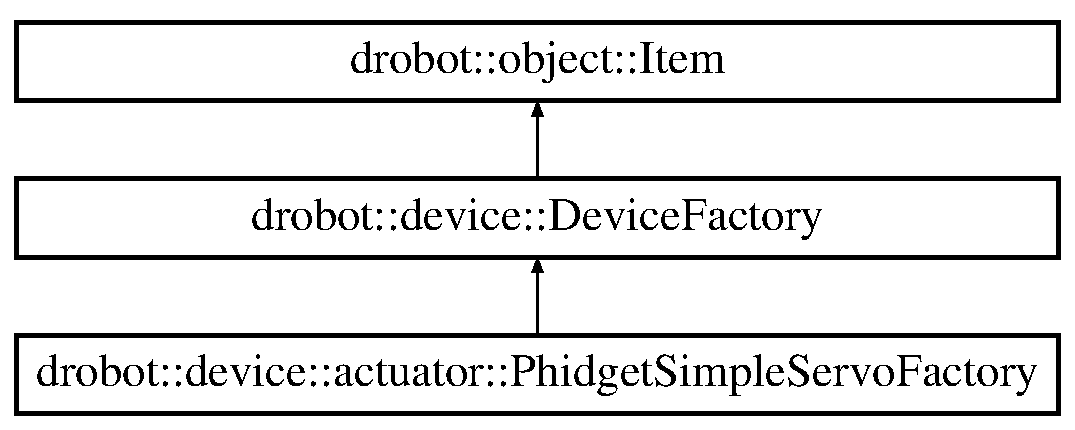
\includegraphics[height=3.000000cm]{classdrobot_1_1device_1_1actuator_1_1PhidgetSimpleServoFactory}
\end{center}
\end{figure}
\subsection*{Public Member Functions}
\begin{DoxyCompactItemize}
\item 
virtual void \hyperlink{classdrobot_1_1device_1_1actuator_1_1PhidgetSimpleServoFactory_a30cab321adc5079711b93fc452028736}{create\-From\-Dom\-Element} (Q\-Dom\-Element element, \hyperlink{classdrobot_1_1robot_1_1Robot}{robot\-::\-Robot} $\ast$robot)
\begin{DoxyCompactList}\small\item\em create\-From\-Dom\-Element \end{DoxyCompactList}\end{DoxyCompactItemize}
\subsection*{Additional Inherited Members}


\subsection{Member Function Documentation}
\hypertarget{classdrobot_1_1device_1_1actuator_1_1PhidgetSimpleServoFactory_a30cab321adc5079711b93fc452028736}{\index{drobot\-::device\-::actuator\-::\-Phidget\-Simple\-Servo\-Factory@{drobot\-::device\-::actuator\-::\-Phidget\-Simple\-Servo\-Factory}!create\-From\-Dom\-Element@{create\-From\-Dom\-Element}}
\index{create\-From\-Dom\-Element@{create\-From\-Dom\-Element}!drobot::device::actuator::PhidgetSimpleServoFactory@{drobot\-::device\-::actuator\-::\-Phidget\-Simple\-Servo\-Factory}}
\subsubsection[{create\-From\-Dom\-Element}]{\setlength{\rightskip}{0pt plus 5cm}void drobot\-::device\-::actuator\-::\-Phidget\-Simple\-Servo\-Factory\-::create\-From\-Dom\-Element (
\begin{DoxyParamCaption}
\item[{Q\-Dom\-Element}]{element, }
\item[{{\bf robot\-::\-Robot} $\ast$}]{robot}
\end{DoxyParamCaption}
)\hspace{0.3cm}{\ttfamily [virtual]}}}\label{classdrobot_1_1device_1_1actuator_1_1PhidgetSimpleServoFactory_a30cab321adc5079711b93fc452028736}


create\-From\-Dom\-Element 


\begin{DoxyParams}{Parameters}
{\em element} & \\
\hline
{\em robot} & \\
\hline
\end{DoxyParams}
Creates a device from a Q\-Dom\-Element. This method should add the device of the robots \hyperlink{classdrobot_1_1device_1_1DeviceManager}{Device\-Manager}. If the created \hyperlink{classdrobot_1_1device_1_1Device}{Device} is a Controller the controller property of the robot should also be set. Each device element may contain channel elements which have to be parsed by the channel\-Factories. Also if the device have need of a \hyperlink{classdrobot_1_1device_1_1DeviceBoard}{Device\-Board} it should be added to the \hyperlink{classdrobot_1_1device_1_1DeviceManager}{Device\-Manager} too. See actuator/phidgetadvancedservofactory.\-cpp for an example. 

Implements \hyperlink{classdrobot_1_1device_1_1DeviceFactory_af9234abdb75d5a0129630baabe0c98cc}{drobot\-::device\-::\-Device\-Factory}.



The documentation for this class was generated from the following files\-:\begin{DoxyCompactItemize}
\item 
src/drobot/device/actuator/phidgetsimpleservofactory.\-h\item 
src/drobot/device/actuator/phidgetsimpleservofactory.\-cpp\end{DoxyCompactItemize}

\hypertarget{classdrobot_1_1device_1_1vestibular_1_1PhidgetVestibular}{\section{drobot\-:\-:device\-:\-:vestibular\-:\-:Phidget\-Vestibular Class Reference}
\label{classdrobot_1_1device_1_1vestibular_1_1PhidgetVestibular}\index{drobot\-::device\-::vestibular\-::\-Phidget\-Vestibular@{drobot\-::device\-::vestibular\-::\-Phidget\-Vestibular}}
}


The \hyperlink{classdrobot_1_1device_1_1vestibular_1_1PhidgetVestibular}{Phidget\-Vestibular} class represents a Phidget Spatial module.  




{\ttfamily \#include $<$phidgetvestibular.\-h$>$}

Inheritance diagram for drobot\-:\-:device\-:\-:vestibular\-:\-:Phidget\-Vestibular\-:\begin{figure}[H]
\begin{center}
\leavevmode
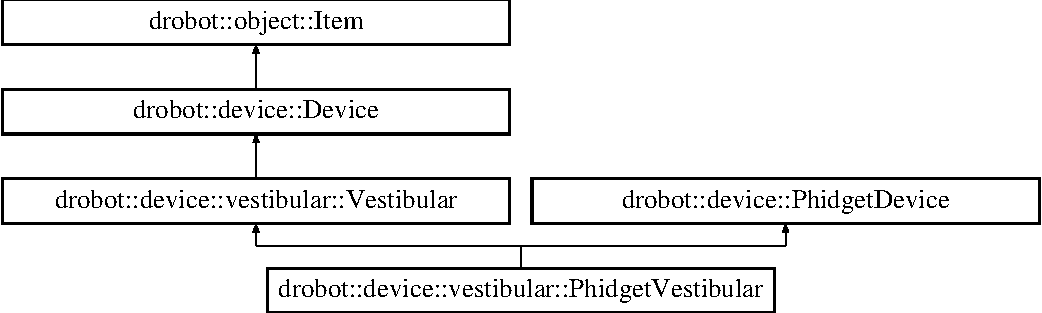
\includegraphics[height=4.000000cm]{classdrobot_1_1device_1_1vestibular_1_1PhidgetVestibular}
\end{center}
\end{figure}
\subsection*{Public Member Functions}
\begin{DoxyCompactItemize}
\item 
\hypertarget{classdrobot_1_1device_1_1vestibular_1_1PhidgetVestibular_ab55a9ea87ecb65d414d09841d2113acf}{{\bfseries Phidget\-Vestibular} (std\-::string name)}\label{classdrobot_1_1device_1_1vestibular_1_1PhidgetVestibular_ab55a9ea87ecb65d414d09841d2113acf}

\item 
\hypertarget{classdrobot_1_1device_1_1vestibular_1_1PhidgetVestibular_a2736f1b981aac44e03e97f06351efd24}{{\bfseries Phidget\-Vestibular} (std\-::string name, int serial)}\label{classdrobot_1_1device_1_1vestibular_1_1PhidgetVestibular_a2736f1b981aac44e03e97f06351efd24}

\item 
\hypertarget{classdrobot_1_1device_1_1vestibular_1_1PhidgetVestibular_abe2423ad121ae794fb7c0301f1baa185}{{\bfseries Phidget\-Vestibular} (std\-::string name, C\-Phidget\-Spatial\-Handle phidget\-Handle)}\label{classdrobot_1_1device_1_1vestibular_1_1PhidgetVestibular_abe2423ad121ae794fb7c0301f1baa185}

\item 
\hypertarget{classdrobot_1_1device_1_1vestibular_1_1PhidgetVestibular_a50525a601dd2fda430ed3c4dd1f9806b}{int {\bfseries get\-Acceleration\-Axis\-Count} ()}\label{classdrobot_1_1device_1_1vestibular_1_1PhidgetVestibular_a50525a601dd2fda430ed3c4dd1f9806b}

\item 
\hypertarget{classdrobot_1_1device_1_1vestibular_1_1PhidgetVestibular_a26b31bd12161bbf3cce93947cf91e948}{int {\bfseries get\-Gyro\-Axis\-Count} ()}\label{classdrobot_1_1device_1_1vestibular_1_1PhidgetVestibular_a26b31bd12161bbf3cce93947cf91e948}

\item 
\hypertarget{classdrobot_1_1device_1_1vestibular_1_1PhidgetVestibular_ae3ac5b15d461db8e8f3cd499c66c7593}{int {\bfseries get\-Compass\-Axis\-Count} ()}\label{classdrobot_1_1device_1_1vestibular_1_1PhidgetVestibular_ae3ac5b15d461db8e8f3cd499c66c7593}

\item 
virtual std\-::vector$<$ double $>$ \hyperlink{classdrobot_1_1device_1_1vestibular_1_1PhidgetVestibular_a70f361e5840a67882a5dfbe486e8c0ad}{get\-Acceleration} ()
\begin{DoxyCompactList}\small\item\em get\-Acceleration \end{DoxyCompactList}\item 
virtual std\-::vector$<$ double $>$ \hyperlink{classdrobot_1_1device_1_1vestibular_1_1PhidgetVestibular_a0d4ef25da6879974f9a1d17a611925c0}{get\-Acceleration\-Max} ()
\begin{DoxyCompactList}\small\item\em get\-Acceleration\-Max \end{DoxyCompactList}\item 
virtual std\-::vector$<$ double $>$ \hyperlink{classdrobot_1_1device_1_1vestibular_1_1PhidgetVestibular_a3ce309226cfea7d6f7e863f047b30419}{get\-Acceleration\-Min} ()
\begin{DoxyCompactList}\small\item\em get\-Acceleration\-Min \end{DoxyCompactList}\item 
virtual std\-::vector$<$ double $>$ \hyperlink{classdrobot_1_1device_1_1vestibular_1_1PhidgetVestibular_aa3161475a5ab72949ccfac98d58feebe}{get\-Angular\-Rate} ()
\begin{DoxyCompactList}\small\item\em get\-Angular\-Rate \end{DoxyCompactList}\item 
virtual std\-::vector$<$ double $>$ \hyperlink{classdrobot_1_1device_1_1vestibular_1_1PhidgetVestibular_a8fb6ce7fc0425ffc280971fe75779988}{get\-Angular\-Rate\-Max} ()
\begin{DoxyCompactList}\small\item\em get\-Angular\-Rate\-Max \end{DoxyCompactList}\item 
virtual std\-::vector$<$ double $>$ \hyperlink{classdrobot_1_1device_1_1vestibular_1_1PhidgetVestibular_afeec4d1d479bd7c9bfd2c9efeb8e7f84}{get\-Angular\-Rate\-Min} ()
\begin{DoxyCompactList}\small\item\em get\-Angular\-Rate\-Min \end{DoxyCompactList}\item 
virtual std\-::vector$<$ double $>$ \hyperlink{classdrobot_1_1device_1_1vestibular_1_1PhidgetVestibular_a0ca904d6cbffeb441834f22e8c808b50}{get\-Magnetic\-Field} ()
\begin{DoxyCompactList}\small\item\em get\-Magnetic\-Field \end{DoxyCompactList}\item 
virtual std\-::vector$<$ double $>$ \hyperlink{classdrobot_1_1device_1_1vestibular_1_1PhidgetVestibular_a1281363ecdc21919d04904cb2d3c3e2c}{get\-Magnetic\-Field\-Max} ()
\begin{DoxyCompactList}\small\item\em get\-Magnetic\-Field\-Max \end{DoxyCompactList}\item 
virtual std\-::vector$<$ double $>$ \hyperlink{classdrobot_1_1device_1_1vestibular_1_1PhidgetVestibular_adb71ac894232a61e286e5d374e30d09d}{get\-Magnetic\-Field\-Min} ()
\begin{DoxyCompactList}\small\item\em get\-Magnetic\-Field\-Min \end{DoxyCompactList}\item 
\hypertarget{classdrobot_1_1device_1_1vestibular_1_1PhidgetVestibular_a7d5ff6fbd49ad5754da22a14d6073dec}{void {\bfseries zero\-Gyro} ()}\label{classdrobot_1_1device_1_1vestibular_1_1PhidgetVestibular_a7d5ff6fbd49ad5754da22a14d6073dec}

\item 
\hypertarget{classdrobot_1_1device_1_1vestibular_1_1PhidgetVestibular_a1cbfe1342ff68d9e6c0b1b031e18cc4e}{int {\bfseries get\-Data\-Rate} ()}\label{classdrobot_1_1device_1_1vestibular_1_1PhidgetVestibular_a1cbfe1342ff68d9e6c0b1b031e18cc4e}

\item 
\hypertarget{classdrobot_1_1device_1_1vestibular_1_1PhidgetVestibular_af712368b99f59ea188455fdc4e1318fd}{void {\bfseries set\-Data\-Rate} (int milliseconds)}\label{classdrobot_1_1device_1_1vestibular_1_1PhidgetVestibular_af712368b99f59ea188455fdc4e1318fd}

\item 
\hypertarget{classdrobot_1_1device_1_1vestibular_1_1PhidgetVestibular_ab474df478e3bea1a3c92b76ada0abea8}{int {\bfseries get\-Data\-Rate\-Max} ()}\label{classdrobot_1_1device_1_1vestibular_1_1PhidgetVestibular_ab474df478e3bea1a3c92b76ada0abea8}

\item 
\hypertarget{classdrobot_1_1device_1_1vestibular_1_1PhidgetVestibular_af7265613db2b247eef6db456108388da}{int {\bfseries get\-Data\-Rate\-Min} ()}\label{classdrobot_1_1device_1_1vestibular_1_1PhidgetVestibular_af7265613db2b247eef6db456108388da}

\item 
\hypertarget{classdrobot_1_1device_1_1vestibular_1_1PhidgetVestibular_ac7b70470063bc4cfd8d0d2096610deb9}{void {\bfseries set\-Compass\-Correction\-Parameters} (double magnetic\-Field, std\-::vector$<$ double $>$ offset, std\-::vector$<$ double $>$ gain, std\-::vector$<$ double $>$ T)}\label{classdrobot_1_1device_1_1vestibular_1_1PhidgetVestibular_ac7b70470063bc4cfd8d0d2096610deb9}

\item 
\hypertarget{classdrobot_1_1device_1_1vestibular_1_1PhidgetVestibular_ae8f7d60741e9f7b1ec07824a38347e0d}{void {\bfseries reset\-Compass\-Correction\-Parameters} ()}\label{classdrobot_1_1device_1_1vestibular_1_1PhidgetVestibular_ae8f7d60741e9f7b1ec07824a38347e0d}

\item 
virtual void \hyperlink{classdrobot_1_1device_1_1vestibular_1_1PhidgetVestibular_a23ef10594aaaddb5f3f2a9908b531c23}{enable} ()
\begin{DoxyCompactList}\small\item\em enables the device. \end{DoxyCompactList}\item 
virtual void \hyperlink{classdrobot_1_1device_1_1vestibular_1_1PhidgetVestibular_ae1887d6d36bf2a25925663e35bd6d57d}{disable} ()
\begin{DoxyCompactList}\small\item\em disables the device. \end{DoxyCompactList}\item 
virtual bool \hyperlink{classdrobot_1_1device_1_1vestibular_1_1PhidgetVestibular_aed99fc288425612c447cc0df4938d9cd}{is\-Enabled} ()
\begin{DoxyCompactList}\small\item\em check if the device is enabled \end{DoxyCompactList}\end{DoxyCompactItemize}
\subsection*{Protected Member Functions}
\begin{DoxyCompactItemize}
\item 
virtual C\-Phidget\-Handle \hyperlink{classdrobot_1_1device_1_1vestibular_1_1PhidgetVestibular_a8292d6ebbc1910eca84081cf76bf3afe}{get\-Phidget\-Handle} ()
\begin{DoxyCompactList}\small\item\em Must be implemented by the specific phidget device to return a C\-Phidget\-Handle struct. \end{DoxyCompactList}\end{DoxyCompactItemize}
\subsection*{Private Attributes}
\begin{DoxyCompactItemize}
\item 
\hypertarget{classdrobot_1_1device_1_1vestibular_1_1PhidgetVestibular_a43744d923d0411a76957d12172f5749a}{C\-Phidget\-Spatial\-Handle {\bfseries \-\_\-phidget\-Handle}}\label{classdrobot_1_1device_1_1vestibular_1_1PhidgetVestibular_a43744d923d0411a76957d12172f5749a}

\item 
\hypertarget{classdrobot_1_1device_1_1vestibular_1_1PhidgetVestibular_a5e5ba8b529ed4774c35ff3498416e22e}{bool {\bfseries \-\_\-enabled}}\label{classdrobot_1_1device_1_1vestibular_1_1PhidgetVestibular_a5e5ba8b529ed4774c35ff3498416e22e}

\end{DoxyCompactItemize}
\subsection*{Additional Inherited Members}


\subsection{Detailed Description}
The \hyperlink{classdrobot_1_1device_1_1vestibular_1_1PhidgetVestibular}{Phidget\-Vestibular} class represents a Phidget Spatial module. 

\subsection{Member Function Documentation}
\hypertarget{classdrobot_1_1device_1_1vestibular_1_1PhidgetVestibular_ae1887d6d36bf2a25925663e35bd6d57d}{\index{drobot\-::device\-::vestibular\-::\-Phidget\-Vestibular@{drobot\-::device\-::vestibular\-::\-Phidget\-Vestibular}!disable@{disable}}
\index{disable@{disable}!drobot::device::vestibular::PhidgetVestibular@{drobot\-::device\-::vestibular\-::\-Phidget\-Vestibular}}
\subsubsection[{disable}]{\setlength{\rightskip}{0pt plus 5cm}void drobot\-::device\-::vestibular\-::\-Phidget\-Vestibular\-::disable (
\begin{DoxyParamCaption}
{}
\end{DoxyParamCaption}
)\hspace{0.3cm}{\ttfamily [virtual]}}}\label{classdrobot_1_1device_1_1vestibular_1_1PhidgetVestibular_ae1887d6d36bf2a25925663e35bd6d57d}


disables the device. 

This function has to be implemented by the specific device. For physical devices like actuators this method should power off the device; 

Reimplemented from \hyperlink{classdrobot_1_1device_1_1Device_a289499673ae30bd72101c68fbd04cd89}{drobot\-::device\-::\-Device}.

\hypertarget{classdrobot_1_1device_1_1vestibular_1_1PhidgetVestibular_a23ef10594aaaddb5f3f2a9908b531c23}{\index{drobot\-::device\-::vestibular\-::\-Phidget\-Vestibular@{drobot\-::device\-::vestibular\-::\-Phidget\-Vestibular}!enable@{enable}}
\index{enable@{enable}!drobot::device::vestibular::PhidgetVestibular@{drobot\-::device\-::vestibular\-::\-Phidget\-Vestibular}}
\subsubsection[{enable}]{\setlength{\rightskip}{0pt plus 5cm}void drobot\-::device\-::vestibular\-::\-Phidget\-Vestibular\-::enable (
\begin{DoxyParamCaption}
{}
\end{DoxyParamCaption}
)\hspace{0.3cm}{\ttfamily [virtual]}}}\label{classdrobot_1_1device_1_1vestibular_1_1PhidgetVestibular_a23ef10594aaaddb5f3f2a9908b531c23}


enables the device. 

This function has to be implemented by the specific device. For physical devices like actuators this method should power on the device. 

Reimplemented from \hyperlink{classdrobot_1_1device_1_1Device_a0c28785ff2e79f99b8e9eaefe6749f2b}{drobot\-::device\-::\-Device}.

\hypertarget{classdrobot_1_1device_1_1vestibular_1_1PhidgetVestibular_a70f361e5840a67882a5dfbe486e8c0ad}{\index{drobot\-::device\-::vestibular\-::\-Phidget\-Vestibular@{drobot\-::device\-::vestibular\-::\-Phidget\-Vestibular}!get\-Acceleration@{get\-Acceleration}}
\index{get\-Acceleration@{get\-Acceleration}!drobot::device::vestibular::PhidgetVestibular@{drobot\-::device\-::vestibular\-::\-Phidget\-Vestibular}}
\subsubsection[{get\-Acceleration}]{\setlength{\rightskip}{0pt plus 5cm}std\-::vector$<$ double $>$ drobot\-::device\-::vestibular\-::\-Phidget\-Vestibular\-::get\-Acceleration (
\begin{DoxyParamCaption}
{}
\end{DoxyParamCaption}
)\hspace{0.3cm}{\ttfamily [virtual]}}}\label{classdrobot_1_1device_1_1vestibular_1_1PhidgetVestibular_a70f361e5840a67882a5dfbe486e8c0ad}


get\-Acceleration 

\begin{DoxyReturn}{Returns}
acceleration vector 
\end{DoxyReturn}


Implements \hyperlink{classdrobot_1_1device_1_1vestibular_1_1Vestibular_a603a1a556bc01d05fbcdc152fcac187e}{drobot\-::device\-::vestibular\-::\-Vestibular}.

\hypertarget{classdrobot_1_1device_1_1vestibular_1_1PhidgetVestibular_a0d4ef25da6879974f9a1d17a611925c0}{\index{drobot\-::device\-::vestibular\-::\-Phidget\-Vestibular@{drobot\-::device\-::vestibular\-::\-Phidget\-Vestibular}!get\-Acceleration\-Max@{get\-Acceleration\-Max}}
\index{get\-Acceleration\-Max@{get\-Acceleration\-Max}!drobot::device::vestibular::PhidgetVestibular@{drobot\-::device\-::vestibular\-::\-Phidget\-Vestibular}}
\subsubsection[{get\-Acceleration\-Max}]{\setlength{\rightskip}{0pt plus 5cm}std\-::vector$<$ double $>$ drobot\-::device\-::vestibular\-::\-Phidget\-Vestibular\-::get\-Acceleration\-Max (
\begin{DoxyParamCaption}
{}
\end{DoxyParamCaption}
)\hspace{0.3cm}{\ttfamily [virtual]}}}\label{classdrobot_1_1device_1_1vestibular_1_1PhidgetVestibular_a0d4ef25da6879974f9a1d17a611925c0}


get\-Acceleration\-Max 

\begin{DoxyReturn}{Returns}
max acceleration values for each dimension 
\end{DoxyReturn}


Implements \hyperlink{classdrobot_1_1device_1_1vestibular_1_1Vestibular_a373ed8304b4dce771493da5a1a88de81}{drobot\-::device\-::vestibular\-::\-Vestibular}.

\hypertarget{classdrobot_1_1device_1_1vestibular_1_1PhidgetVestibular_a3ce309226cfea7d6f7e863f047b30419}{\index{drobot\-::device\-::vestibular\-::\-Phidget\-Vestibular@{drobot\-::device\-::vestibular\-::\-Phidget\-Vestibular}!get\-Acceleration\-Min@{get\-Acceleration\-Min}}
\index{get\-Acceleration\-Min@{get\-Acceleration\-Min}!drobot::device::vestibular::PhidgetVestibular@{drobot\-::device\-::vestibular\-::\-Phidget\-Vestibular}}
\subsubsection[{get\-Acceleration\-Min}]{\setlength{\rightskip}{0pt plus 5cm}std\-::vector$<$ double $>$ drobot\-::device\-::vestibular\-::\-Phidget\-Vestibular\-::get\-Acceleration\-Min (
\begin{DoxyParamCaption}
{}
\end{DoxyParamCaption}
)\hspace{0.3cm}{\ttfamily [virtual]}}}\label{classdrobot_1_1device_1_1vestibular_1_1PhidgetVestibular_a3ce309226cfea7d6f7e863f047b30419}


get\-Acceleration\-Min 

\begin{DoxyReturn}{Returns}
min acceleration values for each dimension 
\end{DoxyReturn}


Implements \hyperlink{classdrobot_1_1device_1_1vestibular_1_1Vestibular_aa8b4a963dabe11f217e6ec3f589b67c9}{drobot\-::device\-::vestibular\-::\-Vestibular}.

\hypertarget{classdrobot_1_1device_1_1vestibular_1_1PhidgetVestibular_aa3161475a5ab72949ccfac98d58feebe}{\index{drobot\-::device\-::vestibular\-::\-Phidget\-Vestibular@{drobot\-::device\-::vestibular\-::\-Phidget\-Vestibular}!get\-Angular\-Rate@{get\-Angular\-Rate}}
\index{get\-Angular\-Rate@{get\-Angular\-Rate}!drobot::device::vestibular::PhidgetVestibular@{drobot\-::device\-::vestibular\-::\-Phidget\-Vestibular}}
\subsubsection[{get\-Angular\-Rate}]{\setlength{\rightskip}{0pt plus 5cm}std\-::vector$<$ double $>$ drobot\-::device\-::vestibular\-::\-Phidget\-Vestibular\-::get\-Angular\-Rate (
\begin{DoxyParamCaption}
{}
\end{DoxyParamCaption}
)\hspace{0.3cm}{\ttfamily [virtual]}}}\label{classdrobot_1_1device_1_1vestibular_1_1PhidgetVestibular_aa3161475a5ab72949ccfac98d58feebe}


get\-Angular\-Rate 

\begin{DoxyReturn}{Returns}
angular\-Rate vector 
\end{DoxyReturn}


Implements \hyperlink{classdrobot_1_1device_1_1vestibular_1_1Vestibular_adcd46ff2d7971a57550b4221c268eb93}{drobot\-::device\-::vestibular\-::\-Vestibular}.

\hypertarget{classdrobot_1_1device_1_1vestibular_1_1PhidgetVestibular_a8fb6ce7fc0425ffc280971fe75779988}{\index{drobot\-::device\-::vestibular\-::\-Phidget\-Vestibular@{drobot\-::device\-::vestibular\-::\-Phidget\-Vestibular}!get\-Angular\-Rate\-Max@{get\-Angular\-Rate\-Max}}
\index{get\-Angular\-Rate\-Max@{get\-Angular\-Rate\-Max}!drobot::device::vestibular::PhidgetVestibular@{drobot\-::device\-::vestibular\-::\-Phidget\-Vestibular}}
\subsubsection[{get\-Angular\-Rate\-Max}]{\setlength{\rightskip}{0pt plus 5cm}std\-::vector$<$ double $>$ drobot\-::device\-::vestibular\-::\-Phidget\-Vestibular\-::get\-Angular\-Rate\-Max (
\begin{DoxyParamCaption}
{}
\end{DoxyParamCaption}
)\hspace{0.3cm}{\ttfamily [virtual]}}}\label{classdrobot_1_1device_1_1vestibular_1_1PhidgetVestibular_a8fb6ce7fc0425ffc280971fe75779988}


get\-Angular\-Rate\-Max 

\begin{DoxyReturn}{Returns}
max angular\-Rate values for each dimension 
\end{DoxyReturn}


Implements \hyperlink{classdrobot_1_1device_1_1vestibular_1_1Vestibular_aa8b14d53824fab9b37d1009a43d2000f}{drobot\-::device\-::vestibular\-::\-Vestibular}.

\hypertarget{classdrobot_1_1device_1_1vestibular_1_1PhidgetVestibular_afeec4d1d479bd7c9bfd2c9efeb8e7f84}{\index{drobot\-::device\-::vestibular\-::\-Phidget\-Vestibular@{drobot\-::device\-::vestibular\-::\-Phidget\-Vestibular}!get\-Angular\-Rate\-Min@{get\-Angular\-Rate\-Min}}
\index{get\-Angular\-Rate\-Min@{get\-Angular\-Rate\-Min}!drobot::device::vestibular::PhidgetVestibular@{drobot\-::device\-::vestibular\-::\-Phidget\-Vestibular}}
\subsubsection[{get\-Angular\-Rate\-Min}]{\setlength{\rightskip}{0pt plus 5cm}std\-::vector$<$ double $>$ drobot\-::device\-::vestibular\-::\-Phidget\-Vestibular\-::get\-Angular\-Rate\-Min (
\begin{DoxyParamCaption}
{}
\end{DoxyParamCaption}
)\hspace{0.3cm}{\ttfamily [virtual]}}}\label{classdrobot_1_1device_1_1vestibular_1_1PhidgetVestibular_afeec4d1d479bd7c9bfd2c9efeb8e7f84}


get\-Angular\-Rate\-Min 

\begin{DoxyReturn}{Returns}
min angular\-Rate values for each dimension 
\end{DoxyReturn}


Implements \hyperlink{classdrobot_1_1device_1_1vestibular_1_1Vestibular_ad49879a49bf891eaf8aa31127a05f69c}{drobot\-::device\-::vestibular\-::\-Vestibular}.

\hypertarget{classdrobot_1_1device_1_1vestibular_1_1PhidgetVestibular_a0ca904d6cbffeb441834f22e8c808b50}{\index{drobot\-::device\-::vestibular\-::\-Phidget\-Vestibular@{drobot\-::device\-::vestibular\-::\-Phidget\-Vestibular}!get\-Magnetic\-Field@{get\-Magnetic\-Field}}
\index{get\-Magnetic\-Field@{get\-Magnetic\-Field}!drobot::device::vestibular::PhidgetVestibular@{drobot\-::device\-::vestibular\-::\-Phidget\-Vestibular}}
\subsubsection[{get\-Magnetic\-Field}]{\setlength{\rightskip}{0pt plus 5cm}std\-::vector$<$ double $>$ drobot\-::device\-::vestibular\-::\-Phidget\-Vestibular\-::get\-Magnetic\-Field (
\begin{DoxyParamCaption}
{}
\end{DoxyParamCaption}
)\hspace{0.3cm}{\ttfamily [virtual]}}}\label{classdrobot_1_1device_1_1vestibular_1_1PhidgetVestibular_a0ca904d6cbffeb441834f22e8c808b50}


get\-Magnetic\-Field 

\begin{DoxyReturn}{Returns}
magnetic\-Field vector 
\end{DoxyReturn}


Implements \hyperlink{classdrobot_1_1device_1_1vestibular_1_1Vestibular_af916767f525fde239401392308ebdd2d}{drobot\-::device\-::vestibular\-::\-Vestibular}.

\hypertarget{classdrobot_1_1device_1_1vestibular_1_1PhidgetVestibular_a1281363ecdc21919d04904cb2d3c3e2c}{\index{drobot\-::device\-::vestibular\-::\-Phidget\-Vestibular@{drobot\-::device\-::vestibular\-::\-Phidget\-Vestibular}!get\-Magnetic\-Field\-Max@{get\-Magnetic\-Field\-Max}}
\index{get\-Magnetic\-Field\-Max@{get\-Magnetic\-Field\-Max}!drobot::device::vestibular::PhidgetVestibular@{drobot\-::device\-::vestibular\-::\-Phidget\-Vestibular}}
\subsubsection[{get\-Magnetic\-Field\-Max}]{\setlength{\rightskip}{0pt plus 5cm}std\-::vector$<$ double $>$ drobot\-::device\-::vestibular\-::\-Phidget\-Vestibular\-::get\-Magnetic\-Field\-Max (
\begin{DoxyParamCaption}
{}
\end{DoxyParamCaption}
)\hspace{0.3cm}{\ttfamily [virtual]}}}\label{classdrobot_1_1device_1_1vestibular_1_1PhidgetVestibular_a1281363ecdc21919d04904cb2d3c3e2c}


get\-Magnetic\-Field\-Max 

\begin{DoxyReturn}{Returns}
max magnetic\-Field values for each dimension 
\end{DoxyReturn}


Implements \hyperlink{classdrobot_1_1device_1_1vestibular_1_1Vestibular_a47dcc13aab2c15633d25f33c92de035e}{drobot\-::device\-::vestibular\-::\-Vestibular}.

\hypertarget{classdrobot_1_1device_1_1vestibular_1_1PhidgetVestibular_adb71ac894232a61e286e5d374e30d09d}{\index{drobot\-::device\-::vestibular\-::\-Phidget\-Vestibular@{drobot\-::device\-::vestibular\-::\-Phidget\-Vestibular}!get\-Magnetic\-Field\-Min@{get\-Magnetic\-Field\-Min}}
\index{get\-Magnetic\-Field\-Min@{get\-Magnetic\-Field\-Min}!drobot::device::vestibular::PhidgetVestibular@{drobot\-::device\-::vestibular\-::\-Phidget\-Vestibular}}
\subsubsection[{get\-Magnetic\-Field\-Min}]{\setlength{\rightskip}{0pt plus 5cm}std\-::vector$<$ double $>$ drobot\-::device\-::vestibular\-::\-Phidget\-Vestibular\-::get\-Magnetic\-Field\-Min (
\begin{DoxyParamCaption}
{}
\end{DoxyParamCaption}
)\hspace{0.3cm}{\ttfamily [virtual]}}}\label{classdrobot_1_1device_1_1vestibular_1_1PhidgetVestibular_adb71ac894232a61e286e5d374e30d09d}


get\-Magnetic\-Field\-Min 

\begin{DoxyReturn}{Returns}
min magnetic\-Field values for each dimension 
\end{DoxyReturn}


Implements \hyperlink{classdrobot_1_1device_1_1vestibular_1_1Vestibular_aedf3e81c5256febccfc8514fa3368322}{drobot\-::device\-::vestibular\-::\-Vestibular}.

\hypertarget{classdrobot_1_1device_1_1vestibular_1_1PhidgetVestibular_a8292d6ebbc1910eca84081cf76bf3afe}{\index{drobot\-::device\-::vestibular\-::\-Phidget\-Vestibular@{drobot\-::device\-::vestibular\-::\-Phidget\-Vestibular}!get\-Phidget\-Handle@{get\-Phidget\-Handle}}
\index{get\-Phidget\-Handle@{get\-Phidget\-Handle}!drobot::device::vestibular::PhidgetVestibular@{drobot\-::device\-::vestibular\-::\-Phidget\-Vestibular}}
\subsubsection[{get\-Phidget\-Handle}]{\setlength{\rightskip}{0pt plus 5cm}C\-Phidget\-Handle drobot\-::device\-::vestibular\-::\-Phidget\-Vestibular\-::get\-Phidget\-Handle (
\begin{DoxyParamCaption}
{}
\end{DoxyParamCaption}
)\hspace{0.3cm}{\ttfamily [protected]}, {\ttfamily [virtual]}}}\label{classdrobot_1_1device_1_1vestibular_1_1PhidgetVestibular_a8292d6ebbc1910eca84081cf76bf3afe}


Must be implemented by the specific phidget device to return a C\-Phidget\-Handle struct. 

\begin{DoxyReturn}{Returns}

\end{DoxyReturn}


Implements \hyperlink{classdrobot_1_1device_1_1PhidgetDevice_a0bcc3051d4a096d92b428a3166e78861}{drobot\-::device\-::\-Phidget\-Device}.

\hypertarget{classdrobot_1_1device_1_1vestibular_1_1PhidgetVestibular_aed99fc288425612c447cc0df4938d9cd}{\index{drobot\-::device\-::vestibular\-::\-Phidget\-Vestibular@{drobot\-::device\-::vestibular\-::\-Phidget\-Vestibular}!is\-Enabled@{is\-Enabled}}
\index{is\-Enabled@{is\-Enabled}!drobot::device::vestibular::PhidgetVestibular@{drobot\-::device\-::vestibular\-::\-Phidget\-Vestibular}}
\subsubsection[{is\-Enabled}]{\setlength{\rightskip}{0pt plus 5cm}bool drobot\-::device\-::vestibular\-::\-Phidget\-Vestibular\-::is\-Enabled (
\begin{DoxyParamCaption}
{}
\end{DoxyParamCaption}
)\hspace{0.3cm}{\ttfamily [virtual]}}}\label{classdrobot_1_1device_1_1vestibular_1_1PhidgetVestibular_aed99fc288425612c447cc0df4938d9cd}


check if the device is enabled 

\begin{DoxyReturn}{Returns}
true if enabled else false
\end{DoxyReturn}
While the \hyperlink{classdrobot_1_1robot_1_1Robot}{drobot\-::robot\-::\-Robot} is running this property is checked to see whether the device should be used or not. 

Implements \hyperlink{classdrobot_1_1device_1_1Device_aa5b7eac8638d0d2d5ee9bf10607b100e}{drobot\-::device\-::\-Device}.



The documentation for this class was generated from the following files\-:\begin{DoxyCompactItemize}
\item 
/home/imanol/workspace/drobot/new/src/drobot/device/vestibular/phidgetvestibular.\-h\item 
/home/imanol/workspace/drobot/new/src/drobot/device/vestibular/phidgetvestibular.\-cpp\end{DoxyCompactItemize}

\hypertarget{classdrobot_1_1device_1_1vestibular_1_1PhidgetVestibularFactory}{\section{drobot\-:\-:device\-:\-:vestibular\-:\-:Phidget\-Vestibular\-Factory Class Reference}
\label{classdrobot_1_1device_1_1vestibular_1_1PhidgetVestibularFactory}\index{drobot\-::device\-::vestibular\-::\-Phidget\-Vestibular\-Factory@{drobot\-::device\-::vestibular\-::\-Phidget\-Vestibular\-Factory}}
}
Inheritance diagram for drobot\-:\-:device\-:\-:vestibular\-:\-:Phidget\-Vestibular\-Factory\-:\begin{figure}[H]
\begin{center}
\leavevmode
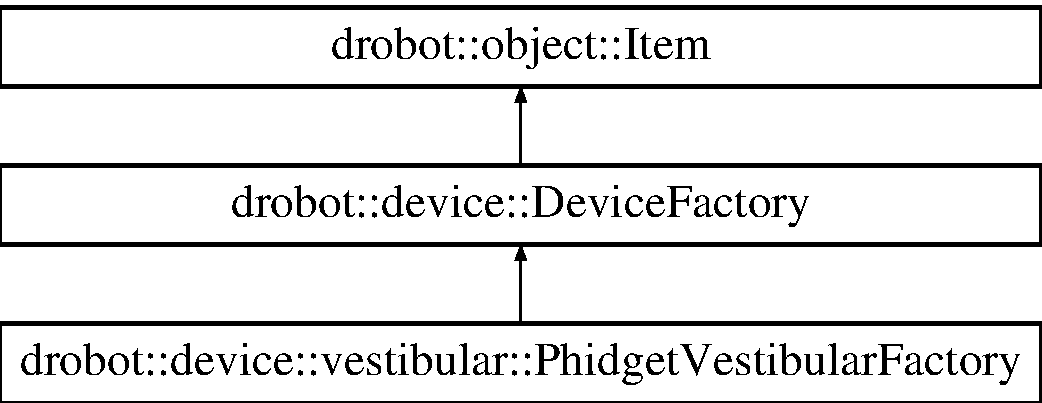
\includegraphics[height=3.000000cm]{classdrobot_1_1device_1_1vestibular_1_1PhidgetVestibularFactory}
\end{center}
\end{figure}
\subsection*{Public Member Functions}
\begin{DoxyCompactItemize}
\item 
virtual void \hyperlink{classdrobot_1_1device_1_1vestibular_1_1PhidgetVestibularFactory_ae877ec4a20bcd09fed94f00952b41f7d}{create\-From\-Dom\-Element} (Q\-Dom\-Element element, \hyperlink{classdrobot_1_1robot_1_1Robot}{robot\-::\-Robot} $\ast$robot)
\begin{DoxyCompactList}\small\item\em create\-From\-Dom\-Element \end{DoxyCompactList}\end{DoxyCompactItemize}
\subsection*{Additional Inherited Members}


\subsection{Member Function Documentation}
\hypertarget{classdrobot_1_1device_1_1vestibular_1_1PhidgetVestibularFactory_ae877ec4a20bcd09fed94f00952b41f7d}{\index{drobot\-::device\-::vestibular\-::\-Phidget\-Vestibular\-Factory@{drobot\-::device\-::vestibular\-::\-Phidget\-Vestibular\-Factory}!create\-From\-Dom\-Element@{create\-From\-Dom\-Element}}
\index{create\-From\-Dom\-Element@{create\-From\-Dom\-Element}!drobot::device::vestibular::PhidgetVestibularFactory@{drobot\-::device\-::vestibular\-::\-Phidget\-Vestibular\-Factory}}
\subsubsection[{create\-From\-Dom\-Element}]{\setlength{\rightskip}{0pt plus 5cm}void drobot\-::device\-::vestibular\-::\-Phidget\-Vestibular\-Factory\-::create\-From\-Dom\-Element (
\begin{DoxyParamCaption}
\item[{Q\-Dom\-Element}]{element, }
\item[{{\bf robot\-::\-Robot} $\ast$}]{robot}
\end{DoxyParamCaption}
)\hspace{0.3cm}{\ttfamily [virtual]}}}\label{classdrobot_1_1device_1_1vestibular_1_1PhidgetVestibularFactory_ae877ec4a20bcd09fed94f00952b41f7d}


create\-From\-Dom\-Element 


\begin{DoxyParams}{Parameters}
{\em element} & \\
\hline
{\em robot} & \\
\hline
\end{DoxyParams}
Creates a device from a Q\-Dom\-Element. This method should add the device of the robots \hyperlink{classdrobot_1_1device_1_1DeviceManager}{Device\-Manager}. If the created \hyperlink{classdrobot_1_1device_1_1Device}{Device} is a Controller the controller property of the robot should also be set. Each device element may contain channel elements which have to be parsed by the channel\-Factories. Also if the device have need of a \hyperlink{classdrobot_1_1device_1_1DeviceBoard}{Device\-Board} it should be added to the \hyperlink{classdrobot_1_1device_1_1DeviceManager}{Device\-Manager} too. See actuator/phidgetadvancedservofactory.\-cpp for an example. 

Implements \hyperlink{classdrobot_1_1device_1_1DeviceFactory_af9234abdb75d5a0129630baabe0c98cc}{drobot\-::device\-::\-Device\-Factory}.



The documentation for this class was generated from the following files\-:\begin{DoxyCompactItemize}
\item 
src/drobot/device/vestibular/phidgetvestibularfactory.\-h\item 
src/drobot/device/vestibular/phidgetvestibularfactory.\-cpp\end{DoxyCompactItemize}

\hypertarget{structdrobot_1_1device_1_1vision_1_1Pixel}{\section{drobot\-:\-:device\-:\-:vision\-:\-:Pixel Struct Reference}
\label{structdrobot_1_1device_1_1vision_1_1Pixel}\index{drobot\-::device\-::vision\-::\-Pixel@{drobot\-::device\-::vision\-::\-Pixel}}
}
\subsection*{Public Member Functions}
\begin{DoxyCompactItemize}
\item 
\hypertarget{structdrobot_1_1device_1_1vision_1_1Pixel_afa58aa9520fed71c437a96746d82e2f8}{{\bfseries Pixel} (int red, int green, int blue)}\label{structdrobot_1_1device_1_1vision_1_1Pixel_afa58aa9520fed71c437a96746d82e2f8}

\item 
\hypertarget{structdrobot_1_1device_1_1vision_1_1Pixel_a430772f0631d5286c777c40bbb40a88f}{{\bfseries Pixel} (int brightness)}\label{structdrobot_1_1device_1_1vision_1_1Pixel_a430772f0631d5286c777c40bbb40a88f}

\item 
\hypertarget{structdrobot_1_1device_1_1vision_1_1Pixel_af436a88672b0ddaff3dc333c9ddb113a}{{\bfseries Pixel} (int red, int green, int blue, int brightness)}\label{structdrobot_1_1device_1_1vision_1_1Pixel_af436a88672b0ddaff3dc333c9ddb113a}

\end{DoxyCompactItemize}
\subsection*{Public Attributes}
\begin{DoxyCompactItemize}
\item 
\hypertarget{structdrobot_1_1device_1_1vision_1_1Pixel_a265c4e311e5ea3c42b73868508a0f9fd}{int {\bfseries red}}\label{structdrobot_1_1device_1_1vision_1_1Pixel_a265c4e311e5ea3c42b73868508a0f9fd}

\item 
\hypertarget{structdrobot_1_1device_1_1vision_1_1Pixel_a6d57169f3294c397ecd9c25c30d4adae}{int {\bfseries green}}\label{structdrobot_1_1device_1_1vision_1_1Pixel_a6d57169f3294c397ecd9c25c30d4adae}

\item 
\hypertarget{structdrobot_1_1device_1_1vision_1_1Pixel_abb8ae018ebff8e8a5100006cbcf2e81d}{int {\bfseries blue}}\label{structdrobot_1_1device_1_1vision_1_1Pixel_abb8ae018ebff8e8a5100006cbcf2e81d}

\item 
\hypertarget{structdrobot_1_1device_1_1vision_1_1Pixel_ab6662ba55e20dce08e7c301eae98a934}{int {\bfseries brightness}}\label{structdrobot_1_1device_1_1vision_1_1Pixel_ab6662ba55e20dce08e7c301eae98a934}

\end{DoxyCompactItemize}


The documentation for this struct was generated from the following file\-:\begin{DoxyCompactItemize}
\item 
/home/imanol/workspace/drobot/new/src/drobot/device/vision/pixel.\-h\end{DoxyCompactItemize}

\hypertarget{classdrobot_1_1experiment_1_1tactileTest_1_1program_1_1Program}{\section{drobot\-:\-:experiment\-:\-:tactile\-Test\-:\-:program\-:\-:Program Class Reference}
\label{classdrobot_1_1experiment_1_1tactileTest_1_1program_1_1Program}\index{drobot\-::experiment\-::tactile\-Test\-::program\-::\-Program@{drobot\-::experiment\-::tactile\-Test\-::program\-::\-Program}}
}
Inheritance diagram for drobot\-:\-:experiment\-:\-:tactile\-Test\-:\-:program\-:\-:Program\-:\begin{figure}[H]
\begin{center}
\leavevmode
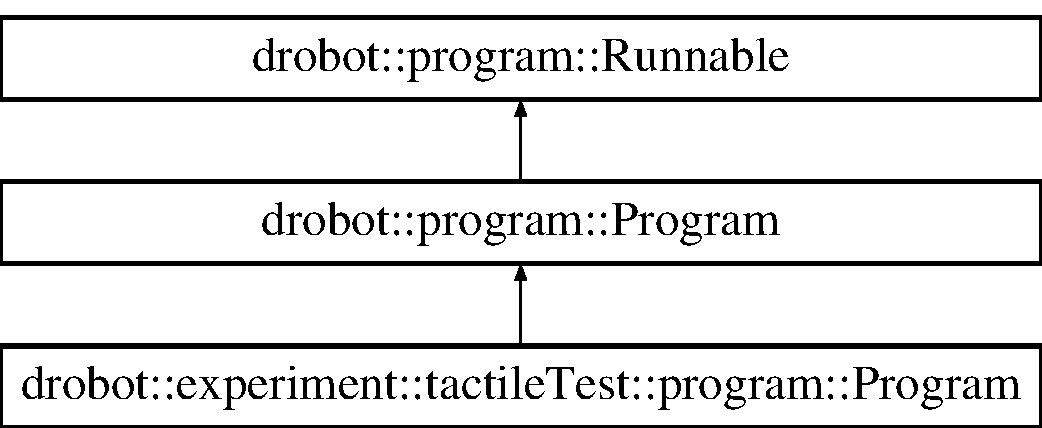
\includegraphics[height=3.000000cm]{classdrobot_1_1experiment_1_1tactileTest_1_1program_1_1Program}
\end{center}
\end{figure}
\subsection*{Public Member Functions}
\begin{DoxyCompactItemize}
\item 
\hypertarget{classdrobot_1_1experiment_1_1tactileTest_1_1program_1_1Program_aa5f0d003909831299df4b658a15c9b22}{{\bfseries Program} (std\-::string name)}\label{classdrobot_1_1experiment_1_1tactileTest_1_1program_1_1Program_aa5f0d003909831299df4b658a15c9b22}

\item 
\hypertarget{classdrobot_1_1experiment_1_1tactileTest_1_1program_1_1Program_a6b9cfdd2d5bb66558836f8c404cfc701}{virtual void \hyperlink{classdrobot_1_1experiment_1_1tactileTest_1_1program_1_1Program_a6b9cfdd2d5bb66558836f8c404cfc701}{run} ()}\label{classdrobot_1_1experiment_1_1tactileTest_1_1program_1_1Program_a6b9cfdd2d5bb66558836f8c404cfc701}

\begin{DoxyCompactList}\small\item\em run has to be implemented by the child class. It should periodically check if \hyperlink{classdrobot_1_1program_1_1Runnable_ab22aef578839f56051702094b6f768df}{is\-Running()} still returns true. If it returns false the program should abort. \end{DoxyCompactList}\item 
virtual Q\-Widget $\ast$ \hyperlink{classdrobot_1_1experiment_1_1tactileTest_1_1program_1_1Program_a63c70e8e24bfc651d3be41680590303d}{get\-Widget} ()
\begin{DoxyCompactList}\small\item\em get\-Widget. This method returns a widget for this program containing its G\-U\-I. \end{DoxyCompactList}\end{DoxyCompactItemize}
\subsection*{Private Attributes}
\begin{DoxyCompactItemize}
\item 
\hypertarget{classdrobot_1_1experiment_1_1tactileTest_1_1program_1_1Program_a4b64dccea8a96670dcd7beb974883121}{\hyperlink{classdrobot_1_1robot_1_1Robot}{drobot\-::robot\-::\-Robot} {\bfseries \-\_\-robo}}\label{classdrobot_1_1experiment_1_1tactileTest_1_1program_1_1Program_a4b64dccea8a96670dcd7beb974883121}

\end{DoxyCompactItemize}
\subsection*{Additional Inherited Members}


\subsection{Member Function Documentation}
\hypertarget{classdrobot_1_1experiment_1_1tactileTest_1_1program_1_1Program_a63c70e8e24bfc651d3be41680590303d}{\index{drobot\-::experiment\-::tactile\-Test\-::program\-::\-Program@{drobot\-::experiment\-::tactile\-Test\-::program\-::\-Program}!get\-Widget@{get\-Widget}}
\index{get\-Widget@{get\-Widget}!drobot::experiment::tactileTest::program::Program@{drobot\-::experiment\-::tactile\-Test\-::program\-::\-Program}}
\subsubsection[{get\-Widget}]{\setlength{\rightskip}{0pt plus 5cm}Q\-Widget $\ast$ drobot\-::experiment\-::tactile\-Test\-::program\-::\-Program\-::get\-Widget (
\begin{DoxyParamCaption}
{}
\end{DoxyParamCaption}
)\hspace{0.3cm}{\ttfamily [virtual]}}}\label{classdrobot_1_1experiment_1_1tactileTest_1_1program_1_1Program_a63c70e8e24bfc651d3be41680590303d}


get\-Widget. This method returns a widget for this program containing its G\-U\-I. 

\begin{DoxyReturn}{Returns}
the widget 
\end{DoxyReturn}


Implements \hyperlink{classdrobot_1_1program_1_1Program_a488b539642af7dbc51a2a8562a5fb33b}{drobot\-::program\-::\-Program}.



The documentation for this class was generated from the following files\-:\begin{DoxyCompactItemize}
\item 
/home/imanol/workspace/drobot/new/src/drobot/experiment/tactile\-Test/program/tactiletestprogram.\-h\item 
/home/imanol/workspace/drobot/new/src/drobot/experiment/tactile\-Test/program/tactiletestprogram.\-cpp\end{DoxyCompactItemize}

\hypertarget{classdrobot_1_1program_1_1Program}{\section{drobot\-:\-:program\-:\-:Program Class Reference}
\label{classdrobot_1_1program_1_1Program}\index{drobot\-::program\-::\-Program@{drobot\-::program\-::\-Program}}
}


The \hyperlink{classdrobot_1_1program_1_1Program}{Program} class represents a running program and serves as a base class. It has a G\-U\-I associated with it. See \hyperlink{classdrobot_1_1program_1_1Program_a488b539642af7dbc51a2a8562a5fb33b}{get\-Widget()}.  




{\ttfamily \#include $<$program.\-h$>$}

Inheritance diagram for drobot\-:\-:program\-:\-:Program\-:\begin{figure}[H]
\begin{center}
\leavevmode
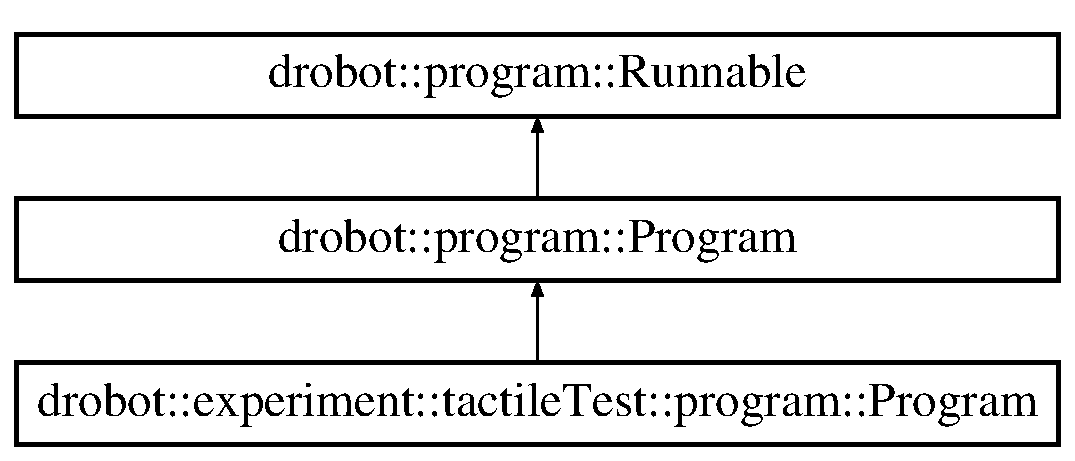
\includegraphics[height=3.000000cm]{classdrobot_1_1program_1_1Program}
\end{center}
\end{figure}
\subsection*{Public Member Functions}
\begin{DoxyCompactItemize}
\item 
\hypertarget{classdrobot_1_1program_1_1Program_ad9c4cb13794de0e6c5f90e155d5e6e57}{{\bfseries Program} (std\-::string name)}\label{classdrobot_1_1program_1_1Program_ad9c4cb13794de0e6c5f90e155d5e6e57}

\item 
\hypertarget{classdrobot_1_1program_1_1Program_a7aec4494957e88d290c33de27d1fa623}{std\-::string {\bfseries get\-Name} ()}\label{classdrobot_1_1program_1_1Program_a7aec4494957e88d290c33de27d1fa623}

\item 
\hypertarget{classdrobot_1_1program_1_1Program_ab69fd00918f24938a6289bf170c65c63}{void {\bfseries set\-Name} (std\-::string name)}\label{classdrobot_1_1program_1_1Program_ab69fd00918f24938a6289bf170c65c63}

\item 
virtual Q\-Widget $\ast$ \hyperlink{classdrobot_1_1program_1_1Program_a488b539642af7dbc51a2a8562a5fb33b}{get\-Widget} ()=0
\begin{DoxyCompactList}\small\item\em get\-Widget. This method returns a widget for this program containing its G\-U\-I. \end{DoxyCompactList}\end{DoxyCompactItemize}
\subsection*{Protected Attributes}
\begin{DoxyCompactItemize}
\item 
\hypertarget{classdrobot_1_1program_1_1Program_a15ba1b38a91d9071f66c080304c9647e}{Q\-Widget $\ast$ {\bfseries \-\_\-widget}}\label{classdrobot_1_1program_1_1Program_a15ba1b38a91d9071f66c080304c9647e}

\item 
\hypertarget{classdrobot_1_1program_1_1Program_a156382ab4c4d2a1713719f7762604f01}{std\-::string {\bfseries \-\_\-name}}\label{classdrobot_1_1program_1_1Program_a156382ab4c4d2a1713719f7762604f01}

\end{DoxyCompactItemize}


\subsection{Detailed Description}
The \hyperlink{classdrobot_1_1program_1_1Program}{Program} class represents a running program and serves as a base class. It has a G\-U\-I associated with it. See \hyperlink{classdrobot_1_1program_1_1Program_a488b539642af7dbc51a2a8562a5fb33b}{get\-Widget()}. 

\subsection{Member Function Documentation}
\hypertarget{classdrobot_1_1program_1_1Program_a488b539642af7dbc51a2a8562a5fb33b}{\index{drobot\-::program\-::\-Program@{drobot\-::program\-::\-Program}!get\-Widget@{get\-Widget}}
\index{get\-Widget@{get\-Widget}!drobot::program::Program@{drobot\-::program\-::\-Program}}
\subsubsection[{get\-Widget}]{\setlength{\rightskip}{0pt plus 5cm}virtual Q\-Widget$\ast$ drobot\-::program\-::\-Program\-::get\-Widget (
\begin{DoxyParamCaption}
{}
\end{DoxyParamCaption}
)\hspace{0.3cm}{\ttfamily [pure virtual]}}}\label{classdrobot_1_1program_1_1Program_a488b539642af7dbc51a2a8562a5fb33b}


get\-Widget. This method returns a widget for this program containing its G\-U\-I. 

\begin{DoxyReturn}{Returns}
the widget 
\end{DoxyReturn}


Implemented in \hyperlink{classdrobot_1_1experiment_1_1tactileTest_1_1program_1_1Program_a63c70e8e24bfc651d3be41680590303d}{drobot\-::experiment\-::tactile\-Test\-::program\-::\-Program}.



The documentation for this class was generated from the following files\-:\begin{DoxyCompactItemize}
\item 
/home/imanol/workspace/drobot/new/src/drobot/program/program.\-h\item 
/home/imanol/workspace/drobot/new/src/drobot/program/program.\-cpp\end{DoxyCompactItemize}

\hypertarget{classdrobot_1_1experiment_1_1tactileTest_1_1program_1_1ProgramFactory}{\section{drobot\-:\-:experiment\-:\-:tactile\-Test\-:\-:program\-:\-:Program\-Factory Class Reference}
\label{classdrobot_1_1experiment_1_1tactileTest_1_1program_1_1ProgramFactory}\index{drobot\-::experiment\-::tactile\-Test\-::program\-::\-Program\-Factory@{drobot\-::experiment\-::tactile\-Test\-::program\-::\-Program\-Factory}}
}
Inheritance diagram for drobot\-:\-:experiment\-:\-:tactile\-Test\-:\-:program\-:\-:Program\-Factory\-:\begin{figure}[H]
\begin{center}
\leavevmode
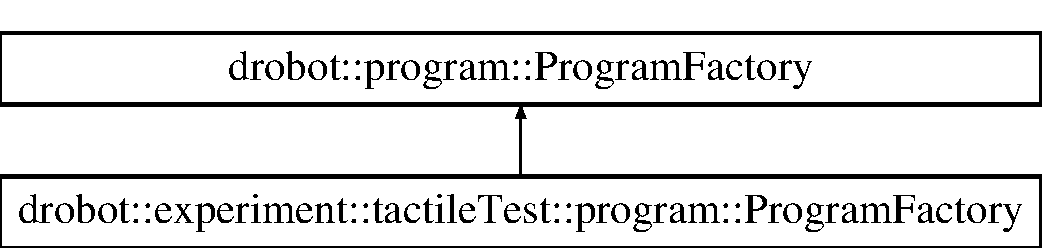
\includegraphics[height=2.000000cm]{classdrobot_1_1experiment_1_1tactileTest_1_1program_1_1ProgramFactory}
\end{center}
\end{figure}
\subsection*{Public Member Functions}
\begin{DoxyCompactItemize}
\item 
virtual \hyperlink{classdrobot_1_1program_1_1Program}{drobot\-::program\-::\-Program} $\ast$ \hyperlink{classdrobot_1_1experiment_1_1tactileTest_1_1program_1_1ProgramFactory_a8a240e973d00cc0cb5389bddd3b927c8}{create\-Instance} ()
\begin{DoxyCompactList}\small\item\em this method should instanciate a new program instance and call \hyperlink{classdrobot_1_1program_1_1ProgramFactory_afba61329928433e93b8cede0d892a55e}{next\-Program\-Name()} to determine it's name. \end{DoxyCompactList}\end{DoxyCompactItemize}
\subsection*{Additional Inherited Members}


\subsection{Member Function Documentation}
\hypertarget{classdrobot_1_1experiment_1_1tactileTest_1_1program_1_1ProgramFactory_a8a240e973d00cc0cb5389bddd3b927c8}{\index{drobot\-::experiment\-::tactile\-Test\-::program\-::\-Program\-Factory@{drobot\-::experiment\-::tactile\-Test\-::program\-::\-Program\-Factory}!create\-Instance@{create\-Instance}}
\index{create\-Instance@{create\-Instance}!drobot::experiment::tactileTest::program::ProgramFactory@{drobot\-::experiment\-::tactile\-Test\-::program\-::\-Program\-Factory}}
\subsubsection[{create\-Instance}]{\setlength{\rightskip}{0pt plus 5cm}{\bf drobot\-::program\-::\-Program} $\ast$ drobot\-::experiment\-::tactile\-Test\-::program\-::\-Program\-Factory\-::create\-Instance (
\begin{DoxyParamCaption}
{}
\end{DoxyParamCaption}
)\hspace{0.3cm}{\ttfamily [virtual]}}}\label{classdrobot_1_1experiment_1_1tactileTest_1_1program_1_1ProgramFactory_a8a240e973d00cc0cb5389bddd3b927c8}


this method should instanciate a new program instance and call \hyperlink{classdrobot_1_1program_1_1ProgramFactory_afba61329928433e93b8cede0d892a55e}{next\-Program\-Name()} to determine it's name. 

\begin{DoxyReturn}{Returns}
\hyperlink{classdrobot_1_1experiment_1_1tactileTest_1_1program_1_1Program}{Program} instance 
\end{DoxyReturn}


Implements \hyperlink{classdrobot_1_1program_1_1ProgramFactory_ac47a7a6390cfb5488ddc4581c6cb9d6f}{drobot\-::program\-::\-Program\-Factory}.



The documentation for this class was generated from the following files\-:\begin{DoxyCompactItemize}
\item 
/home/imanol/workspace/drobot/new/src/drobot/experiment/tactile\-Test/program/tactiletestprogramfactory.\-h\item 
/home/imanol/workspace/drobot/new/src/drobot/experiment/tactile\-Test/program/tactiletestprogramfactory.\-cpp\end{DoxyCompactItemize}

\hypertarget{classdrobot_1_1program_1_1ProgramFactory}{\section{drobot\-:\-:program\-:\-:Program\-Factory Class Reference}
\label{classdrobot_1_1program_1_1ProgramFactory}\index{drobot\-::program\-::\-Program\-Factory@{drobot\-::program\-::\-Program\-Factory}}
}


The \hyperlink{classdrobot_1_1program_1_1ProgramFactory}{Program\-Factory} class is used for launching programs defined by the experimenter.  




{\ttfamily \#include $<$programfactory.\-h$>$}

Inheritance diagram for drobot\-:\-:program\-:\-:Program\-Factory\-:\begin{figure}[H]
\begin{center}
\leavevmode
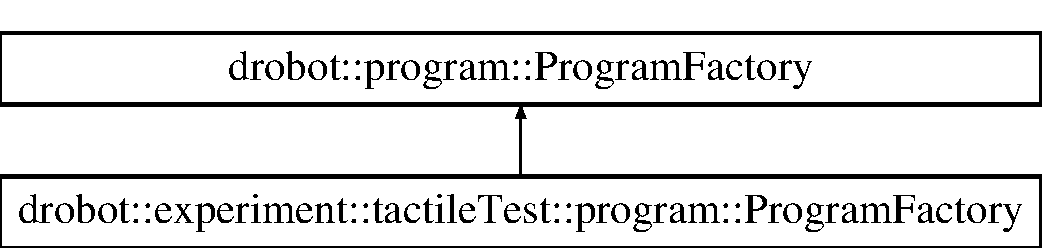
\includegraphics[height=2.000000cm]{classdrobot_1_1program_1_1ProgramFactory}
\end{center}
\end{figure}
\subsection*{Public Member Functions}
\begin{DoxyCompactItemize}
\item 
\hypertarget{classdrobot_1_1program_1_1ProgramFactory_a983aeedad36248a7f669be06640a9d37}{{\bfseries Program\-Factory} (std\-::string name)}\label{classdrobot_1_1program_1_1ProgramFactory_a983aeedad36248a7f669be06640a9d37}

\item 
virtual \hyperlink{classdrobot_1_1program_1_1Program}{Program} $\ast$ \hyperlink{classdrobot_1_1program_1_1ProgramFactory_ac47a7a6390cfb5488ddc4581c6cb9d6f}{create\-Instance} ()=0
\begin{DoxyCompactList}\small\item\em this method should instanciate a new program instance and call \hyperlink{classdrobot_1_1program_1_1ProgramFactory_afba61329928433e93b8cede0d892a55e}{next\-Program\-Name()} to determine it's name. \end{DoxyCompactList}\item 
std\-::string \hyperlink{classdrobot_1_1program_1_1ProgramFactory_aea9163e3cb4901b1d2b517225c5046f7}{get\-Name} ()
\begin{DoxyCompactList}\small\item\em get\-Name. The base name of the programs \end{DoxyCompactList}\item 
std\-::string \hyperlink{classdrobot_1_1program_1_1ProgramFactory_afba61329928433e93b8cede0d892a55e}{next\-Program\-Name} ()
\begin{DoxyCompactList}\small\item\em next\-Program\-Name. Creates a program name for the \hyperlink{classdrobot_1_1program_1_1ProgramFactory_ac47a7a6390cfb5488ddc4581c6cb9d6f}{create\-Instance()} method. \end{DoxyCompactList}\end{DoxyCompactItemize}
\subsection*{Protected Attributes}
\begin{DoxyCompactItemize}
\item 
\hypertarget{classdrobot_1_1program_1_1ProgramFactory_ab956cb5a3106cc177dadc351c47ec8e2}{std\-::string {\bfseries \-\_\-name}}\label{classdrobot_1_1program_1_1ProgramFactory_ab956cb5a3106cc177dadc351c47ec8e2}

\item 
\hypertarget{classdrobot_1_1program_1_1ProgramFactory_aea32ffbc04581a27a823fe520a12c7ce}{int {\bfseries \-\_\-program\-Number}}\label{classdrobot_1_1program_1_1ProgramFactory_aea32ffbc04581a27a823fe520a12c7ce}

\end{DoxyCompactItemize}


\subsection{Detailed Description}
The \hyperlink{classdrobot_1_1program_1_1ProgramFactory}{Program\-Factory} class is used for launching programs defined by the experimenter. 

\subsection{Member Function Documentation}
\hypertarget{classdrobot_1_1program_1_1ProgramFactory_ac47a7a6390cfb5488ddc4581c6cb9d6f}{\index{drobot\-::program\-::\-Program\-Factory@{drobot\-::program\-::\-Program\-Factory}!create\-Instance@{create\-Instance}}
\index{create\-Instance@{create\-Instance}!drobot::program::ProgramFactory@{drobot\-::program\-::\-Program\-Factory}}
\subsubsection[{create\-Instance}]{\setlength{\rightskip}{0pt plus 5cm}virtual {\bf Program}$\ast$ drobot\-::program\-::\-Program\-Factory\-::create\-Instance (
\begin{DoxyParamCaption}
{}
\end{DoxyParamCaption}
)\hspace{0.3cm}{\ttfamily [pure virtual]}}}\label{classdrobot_1_1program_1_1ProgramFactory_ac47a7a6390cfb5488ddc4581c6cb9d6f}


this method should instanciate a new program instance and call \hyperlink{classdrobot_1_1program_1_1ProgramFactory_afba61329928433e93b8cede0d892a55e}{next\-Program\-Name()} to determine it's name. 

\begin{DoxyReturn}{Returns}
\hyperlink{classdrobot_1_1program_1_1Program}{Program} instance 
\end{DoxyReturn}


Implemented in \hyperlink{classdrobot_1_1experiment_1_1tactileTest_1_1program_1_1ProgramFactory_a8a240e973d00cc0cb5389bddd3b927c8}{drobot\-::experiment\-::tactile\-Test\-::program\-::\-Program\-Factory}.

\hypertarget{classdrobot_1_1program_1_1ProgramFactory_aea9163e3cb4901b1d2b517225c5046f7}{\index{drobot\-::program\-::\-Program\-Factory@{drobot\-::program\-::\-Program\-Factory}!get\-Name@{get\-Name}}
\index{get\-Name@{get\-Name}!drobot::program::ProgramFactory@{drobot\-::program\-::\-Program\-Factory}}
\subsubsection[{get\-Name}]{\setlength{\rightskip}{0pt plus 5cm}std\-::string drobot\-::program\-::\-Program\-Factory\-::get\-Name (
\begin{DoxyParamCaption}
{}
\end{DoxyParamCaption}
)}}\label{classdrobot_1_1program_1_1ProgramFactory_aea9163e3cb4901b1d2b517225c5046f7}


get\-Name. The base name of the programs 

\begin{DoxyReturn}{Returns}
the name 
\end{DoxyReturn}
\hypertarget{classdrobot_1_1program_1_1ProgramFactory_afba61329928433e93b8cede0d892a55e}{\index{drobot\-::program\-::\-Program\-Factory@{drobot\-::program\-::\-Program\-Factory}!next\-Program\-Name@{next\-Program\-Name}}
\index{next\-Program\-Name@{next\-Program\-Name}!drobot::program::ProgramFactory@{drobot\-::program\-::\-Program\-Factory}}
\subsubsection[{next\-Program\-Name}]{\setlength{\rightskip}{0pt plus 5cm}std\-::string drobot\-::program\-::\-Program\-Factory\-::next\-Program\-Name (
\begin{DoxyParamCaption}
{}
\end{DoxyParamCaption}
)}}\label{classdrobot_1_1program_1_1ProgramFactory_afba61329928433e93b8cede0d892a55e}


next\-Program\-Name. Creates a program name for the \hyperlink{classdrobot_1_1program_1_1ProgramFactory_ac47a7a6390cfb5488ddc4581c6cb9d6f}{create\-Instance()} method. 

The program name is composed of the base name and an integer. On each call the integer is increased by 1. \begin{DoxyReturn}{Returns}
next program's name 
\end{DoxyReturn}


The documentation for this class was generated from the following files\-:\begin{DoxyCompactItemize}
\item 
src/drobot/program/programfactory.\-h\item 
src/drobot/program/programfactory.\-cpp\end{DoxyCompactItemize}

\hypertarget{classdrobot_1_1program_1_1ProgramManager}{\section{drobot\-:\-:program\-:\-:Program\-Manager Class Reference}
\label{classdrobot_1_1program_1_1ProgramManager}\index{drobot\-::program\-::\-Program\-Manager@{drobot\-::program\-::\-Program\-Manager}}
}


The \hyperlink{classdrobot_1_1program_1_1ProgramManager}{Program\-Manager} class keeps track of the available \hyperlink{classdrobot_1_1program_1_1ProgramFactory}{Program\-Factory} and \hyperlink{classdrobot_1_1program_1_1Program}{Program} instances.  




{\ttfamily \#include $<$programmanager.\-h$>$}

\subsection*{Public Member Functions}
\begin{DoxyCompactItemize}
\item 
void \hyperlink{classdrobot_1_1program_1_1ProgramManager_a4ea28e6c3b74b746364bbc3c2d68bd31}{register\-Program\-Factory} (\hyperlink{classdrobot_1_1program_1_1ProgramFactory}{Program\-Factory} $\ast$program\-Factory)
\begin{DoxyCompactList}\small\item\em register\-Program\-Factory adds a \hyperlink{classdrobot_1_1program_1_1ProgramFactory}{Program\-Factory} \end{DoxyCompactList}\item 
void \hyperlink{classdrobot_1_1program_1_1ProgramManager_a190faf45e5e408b02e0b9858240244ea}{unregister\-Program\-Factory} (\hyperlink{classdrobot_1_1program_1_1ProgramFactory}{Program\-Factory} $\ast$program\-Factory)
\begin{DoxyCompactList}\small\item\em unregister\-Program\-Factory removes a \hyperlink{classdrobot_1_1program_1_1ProgramFactory}{Program\-Factory} \end{DoxyCompactList}\item 
std\-::vector$<$ std\-::string $>$ \hyperlink{classdrobot_1_1program_1_1ProgramManager_a8d67fbed1cdde2f1b0053809e2a35a7b}{list\-Program\-Factory\-Names} ()
\begin{DoxyCompactList}\small\item\em list\-Program\-Factory\-Names \end{DoxyCompactList}\item 
\hyperlink{classdrobot_1_1program_1_1Program}{Program} $\ast$ \hyperlink{classdrobot_1_1program_1_1ProgramManager_adf94bbb6de02d9d304e2776a9e21d40d}{launch\-Program} (std\-::string program\-Name)
\begin{DoxyCompactList}\small\item\em launch\-Program creates a new program instance and starts it. \end{DoxyCompactList}\item 
void \hyperlink{classdrobot_1_1program_1_1ProgramManager_a8ff0772daea03353f6473e041469093a}{kill\-Program} (std\-::string program\-Name)
\begin{DoxyCompactList}\small\item\em kill\-Program cancels a program instance \end{DoxyCompactList}\item 
\hypertarget{classdrobot_1_1program_1_1ProgramManager_a193a85cf0e58c44955513aab1e7253b4}{void \hyperlink{classdrobot_1_1program_1_1ProgramManager_a193a85cf0e58c44955513aab1e7253b4}{kill\-All} ()}\label{classdrobot_1_1program_1_1ProgramManager_a193a85cf0e58c44955513aab1e7253b4}

\begin{DoxyCompactList}\small\item\em kill\-All cancels all program instances \end{DoxyCompactList}\item 
\hypertarget{classdrobot_1_1program_1_1ProgramManager_ad8d36ca3ae149a35055ec65b86a88f2a}{std\-::vector$<$ std\-::string $>$ {\bfseries list\-Program\-Names} ()}\label{classdrobot_1_1program_1_1ProgramManager_ad8d36ca3ae149a35055ec65b86a88f2a}

\end{DoxyCompactItemize}
\subsection*{Private Attributes}
\begin{DoxyCompactItemize}
\item 
\hypertarget{classdrobot_1_1program_1_1ProgramManager_a044432fd5e26ef8f9170d2b6ab726829}{\hyperlink{classdrobot_1_1object_1_1Manager}{object\-::\-Manager}$<$ \hyperlink{classdrobot_1_1program_1_1ProgramFactory}{Program\-Factory} $>$ {\bfseries \-\_\-program\-Factories}}\label{classdrobot_1_1program_1_1ProgramManager_a044432fd5e26ef8f9170d2b6ab726829}

\item 
\hypertarget{classdrobot_1_1program_1_1ProgramManager_a8bf1519b4720d837256c3bb139e56dff}{\hyperlink{classdrobot_1_1object_1_1Manager}{object\-::\-Manager}$<$ \hyperlink{classdrobot_1_1program_1_1Program}{Program} $>$ {\bfseries \-\_\-programs}}\label{classdrobot_1_1program_1_1ProgramManager_a8bf1519b4720d837256c3bb139e56dff}

\end{DoxyCompactItemize}


\subsection{Detailed Description}
The \hyperlink{classdrobot_1_1program_1_1ProgramManager}{Program\-Manager} class keeps track of the available \hyperlink{classdrobot_1_1program_1_1ProgramFactory}{Program\-Factory} and \hyperlink{classdrobot_1_1program_1_1Program}{Program} instances. 

\subsection{Member Function Documentation}
\hypertarget{classdrobot_1_1program_1_1ProgramManager_a8ff0772daea03353f6473e041469093a}{\index{drobot\-::program\-::\-Program\-Manager@{drobot\-::program\-::\-Program\-Manager}!kill\-Program@{kill\-Program}}
\index{kill\-Program@{kill\-Program}!drobot::program::ProgramManager@{drobot\-::program\-::\-Program\-Manager}}
\subsubsection[{kill\-Program}]{\setlength{\rightskip}{0pt plus 5cm}void drobot\-::program\-::\-Program\-Manager\-::kill\-Program (
\begin{DoxyParamCaption}
\item[{std\-::string}]{program\-Name}
\end{DoxyParamCaption}
)}}\label{classdrobot_1_1program_1_1ProgramManager_a8ff0772daea03353f6473e041469093a}


kill\-Program cancels a program instance 


\begin{DoxyParams}{Parameters}
{\em program\-Name} & \\
\hline
\end{DoxyParams}
\hypertarget{classdrobot_1_1program_1_1ProgramManager_adf94bbb6de02d9d304e2776a9e21d40d}{\index{drobot\-::program\-::\-Program\-Manager@{drobot\-::program\-::\-Program\-Manager}!launch\-Program@{launch\-Program}}
\index{launch\-Program@{launch\-Program}!drobot::program::ProgramManager@{drobot\-::program\-::\-Program\-Manager}}
\subsubsection[{launch\-Program}]{\setlength{\rightskip}{0pt plus 5cm}{\bf Program} $\ast$ drobot\-::program\-::\-Program\-Manager\-::launch\-Program (
\begin{DoxyParamCaption}
\item[{std\-::string}]{program\-Name}
\end{DoxyParamCaption}
)}}\label{classdrobot_1_1program_1_1ProgramManager_adf94bbb6de02d9d304e2776a9e21d40d}


launch\-Program creates a new program instance and starts it. 


\begin{DoxyParams}{Parameters}
{\em program\-Name} & is the type of the program to launch \\
\hline
\end{DoxyParams}
\begin{DoxyReturn}{Returns}
the new program instance 
\end{DoxyReturn}
\hypertarget{classdrobot_1_1program_1_1ProgramManager_a8d67fbed1cdde2f1b0053809e2a35a7b}{\index{drobot\-::program\-::\-Program\-Manager@{drobot\-::program\-::\-Program\-Manager}!list\-Program\-Factory\-Names@{list\-Program\-Factory\-Names}}
\index{list\-Program\-Factory\-Names@{list\-Program\-Factory\-Names}!drobot::program::ProgramManager@{drobot\-::program\-::\-Program\-Manager}}
\subsubsection[{list\-Program\-Factory\-Names}]{\setlength{\rightskip}{0pt plus 5cm}std\-::vector$<$ std\-::string $>$ drobot\-::program\-::\-Program\-Manager\-::list\-Program\-Factory\-Names (
\begin{DoxyParamCaption}
{}
\end{DoxyParamCaption}
)}}\label{classdrobot_1_1program_1_1ProgramManager_a8d67fbed1cdde2f1b0053809e2a35a7b}


list\-Program\-Factory\-Names 

\begin{DoxyReturn}{Returns}
the names of the known \hyperlink{classdrobot_1_1program_1_1ProgramFactory}{Program\-Factory} instances 
\end{DoxyReturn}
\hypertarget{classdrobot_1_1program_1_1ProgramManager_a4ea28e6c3b74b746364bbc3c2d68bd31}{\index{drobot\-::program\-::\-Program\-Manager@{drobot\-::program\-::\-Program\-Manager}!register\-Program\-Factory@{register\-Program\-Factory}}
\index{register\-Program\-Factory@{register\-Program\-Factory}!drobot::program::ProgramManager@{drobot\-::program\-::\-Program\-Manager}}
\subsubsection[{register\-Program\-Factory}]{\setlength{\rightskip}{0pt plus 5cm}void drobot\-::program\-::\-Program\-Manager\-::register\-Program\-Factory (
\begin{DoxyParamCaption}
\item[{{\bf Program\-Factory} $\ast$}]{program\-Factory}
\end{DoxyParamCaption}
)}}\label{classdrobot_1_1program_1_1ProgramManager_a4ea28e6c3b74b746364bbc3c2d68bd31}


register\-Program\-Factory adds a \hyperlink{classdrobot_1_1program_1_1ProgramFactory}{Program\-Factory} 


\begin{DoxyParams}{Parameters}
{\em program\-Factory} & \\
\hline
\end{DoxyParams}
\hypertarget{classdrobot_1_1program_1_1ProgramManager_a190faf45e5e408b02e0b9858240244ea}{\index{drobot\-::program\-::\-Program\-Manager@{drobot\-::program\-::\-Program\-Manager}!unregister\-Program\-Factory@{unregister\-Program\-Factory}}
\index{unregister\-Program\-Factory@{unregister\-Program\-Factory}!drobot::program::ProgramManager@{drobot\-::program\-::\-Program\-Manager}}
\subsubsection[{unregister\-Program\-Factory}]{\setlength{\rightskip}{0pt plus 5cm}void drobot\-::program\-::\-Program\-Manager\-::unregister\-Program\-Factory (
\begin{DoxyParamCaption}
\item[{{\bf Program\-Factory} $\ast$}]{program\-Factory}
\end{DoxyParamCaption}
)}}\label{classdrobot_1_1program_1_1ProgramManager_a190faf45e5e408b02e0b9858240244ea}


unregister\-Program\-Factory removes a \hyperlink{classdrobot_1_1program_1_1ProgramFactory}{Program\-Factory} 


\begin{DoxyParams}{Parameters}
{\em program\-Factory} & \\
\hline
\end{DoxyParams}


The documentation for this class was generated from the following files\-:\begin{DoxyCompactItemize}
\item 
src/drobot/program/programmanager.\-h\item 
src/drobot/program/programmanager.\-cpp\end{DoxyCompactItemize}

\hypertarget{classdrobot_1_1robot_1_1Robot}{\section{drobot\-:\-:robot\-:\-:Robot Class Reference}
\label{classdrobot_1_1robot_1_1Robot}\index{drobot\-::robot\-::\-Robot@{drobot\-::robot\-::\-Robot}}
}
Inheritance diagram for drobot\-:\-:robot\-:\-:Robot\-:\begin{figure}[H]
\begin{center}
\leavevmode
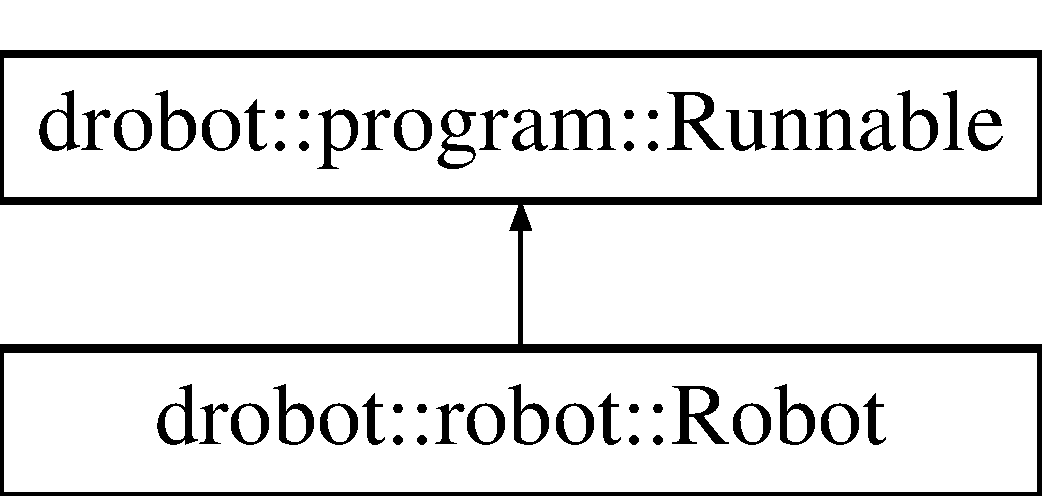
\includegraphics[height=2.000000cm]{classdrobot_1_1robot_1_1Robot}
\end{center}
\end{figure}
\subsection*{Public Member Functions}
\begin{DoxyCompactItemize}
\item 
\hypertarget{classdrobot_1_1robot_1_1Robot_a8f352efdddf1a1d76d3740032964e893}{{\bfseries Robot} (\hyperlink{classdrobot_1_1device_1_1DeviceManager}{device\-::\-Device\-Manager} $\ast$device\-Manager, \hyperlink{classdrobot_1_1robot_1_1Controller}{Controller} $\ast$controller, \hyperlink{classdrobot_1_1event_1_1EventManager}{event\-::\-Event\-Manager} $\ast$event\-Manager, \hyperlink{classdrobot_1_1util_1_1Clock}{util\-::\-Clock} $\ast$clock)}\label{classdrobot_1_1robot_1_1Robot_a8f352efdddf1a1d76d3740032964e893}

\item 
\hypertarget{classdrobot_1_1robot_1_1Robot_a47aad1b040e0c9a1ff8938e13d45473b}{virtual void \hyperlink{classdrobot_1_1robot_1_1Robot_a47aad1b040e0c9a1ff8938e13d45473b}{run} ()}\label{classdrobot_1_1robot_1_1Robot_a47aad1b040e0c9a1ff8938e13d45473b}

\begin{DoxyCompactList}\small\item\em run has to be implemented by the child class. It should periodically check if \hyperlink{classdrobot_1_1program_1_1Runnable_ab22aef578839f56051702094b6f768df}{is\-Running()} still returns true. If it returns false the program should abort. \end{DoxyCompactList}\item 
\hypertarget{classdrobot_1_1robot_1_1Robot_a398ddace28a74ad646a4e390df654c6e}{void {\bfseries set\-Device\-Manager} (\hyperlink{classdrobot_1_1device_1_1DeviceManager}{device\-::\-Device\-Manager} $\ast$device\-Manager)}\label{classdrobot_1_1robot_1_1Robot_a398ddace28a74ad646a4e390df654c6e}

\item 
\hypertarget{classdrobot_1_1robot_1_1Robot_a2aae6dac03338e0af23afc4059cad388}{\hyperlink{classdrobot_1_1device_1_1DeviceManager}{device\-::\-Device\-Manager} $\ast$ {\bfseries get\-Device\-Manager} ()}\label{classdrobot_1_1robot_1_1Robot_a2aae6dac03338e0af23afc4059cad388}

\item 
\hypertarget{classdrobot_1_1robot_1_1Robot_acbd72c93a7535574ccd8a53018b7ac73}{void {\bfseries set\-Controller} (\hyperlink{classdrobot_1_1robot_1_1Controller}{Controller} $\ast$controller)}\label{classdrobot_1_1robot_1_1Robot_acbd72c93a7535574ccd8a53018b7ac73}

\item 
\hypertarget{classdrobot_1_1robot_1_1Robot_a85f58a70090466152bf465ffc945a46b}{\hyperlink{classdrobot_1_1robot_1_1Controller}{Controller} $\ast$ {\bfseries get\-Controller} ()}\label{classdrobot_1_1robot_1_1Robot_a85f58a70090466152bf465ffc945a46b}

\item 
\hypertarget{classdrobot_1_1robot_1_1Robot_a5f3a6d6f9881a5145ad39c3afd7b11ce}{void {\bfseries set\-Event\-Manager} (\hyperlink{classdrobot_1_1event_1_1EventManager}{drobot\-::event\-::\-Event\-Manager} $\ast$event\-Manager)}\label{classdrobot_1_1robot_1_1Robot_a5f3a6d6f9881a5145ad39c3afd7b11ce}

\item 
\hypertarget{classdrobot_1_1robot_1_1Robot_a0fb1145903a7d79467bfbd05cf28e8a5}{\hyperlink{classdrobot_1_1event_1_1EventManager}{drobot\-::event\-::\-Event\-Manager} $\ast$ {\bfseries get\-Event\-Manager} ()}\label{classdrobot_1_1robot_1_1Robot_a0fb1145903a7d79467bfbd05cf28e8a5}

\item 
\hypertarget{classdrobot_1_1robot_1_1Robot_a773b84984f3ff88c0ad1d6c08838e4dc}{void {\bfseries set\-Clock} (\hyperlink{classdrobot_1_1util_1_1Clock}{util\-::\-Clock} $\ast$clock)}\label{classdrobot_1_1robot_1_1Robot_a773b84984f3ff88c0ad1d6c08838e4dc}

\item 
\hypertarget{classdrobot_1_1robot_1_1Robot_a1d5fdac440ebfb5a89a656322a5998ea}{\hyperlink{classdrobot_1_1util_1_1Clock}{util\-::\-Clock} $\ast$ {\bfseries get\-Clock} ()}\label{classdrobot_1_1robot_1_1Robot_a1d5fdac440ebfb5a89a656322a5998ea}

\item 
void \hyperlink{classdrobot_1_1robot_1_1Robot_a3de91af7c152307bf6b38e82ca3ed806}{load\-From\-File} (std\-::string path)
\begin{DoxyCompactList}\small\item\em parse robot from xml file \end{DoxyCompactList}\item 
\hyperlink{classdrobot_1_1object_1_1Manager}{object\-::\-Manager}\\*
$<$ \hyperlink{classdrobot_1_1device_1_1DeviceFactory}{device\-::\-Device\-Factory} $>$ $\ast$ \hyperlink{classdrobot_1_1robot_1_1Robot_a07cb4102e9a93efc68259d3124a3541e}{get\-Device\-Factories} ()
\begin{DoxyCompactList}\small\item\em returns Device\-Factories used for parsing files \end{DoxyCompactList}\end{DoxyCompactItemize}
\subsection*{Private Member Functions}
\begin{DoxyCompactItemize}
\item 
\hypertarget{classdrobot_1_1robot_1_1Robot_aaf3e6c071cde549bfdbb493ef0893af8}{void {\bfseries parse\-Element} (Q\-Dom\-Element element)}\label{classdrobot_1_1robot_1_1Robot_aaf3e6c071cde549bfdbb493ef0893af8}

\item 
\hypertarget{classdrobot_1_1robot_1_1Robot_a08c5f6468f7a655c8d5e06ffa1248cae}{void {\bfseries parse\-Device\-Group} (Q\-Dom\-Element element)}\label{classdrobot_1_1robot_1_1Robot_a08c5f6468f7a655c8d5e06ffa1248cae}

\item 
\hypertarget{classdrobot_1_1robot_1_1Robot_ab9bc0cc2a3e31f026024659ad3d17dd1}{void {\bfseries parse\-Device} (Q\-Dom\-Element element)}\label{classdrobot_1_1robot_1_1Robot_ab9bc0cc2a3e31f026024659ad3d17dd1}

\item 
\hypertarget{classdrobot_1_1robot_1_1Robot_a8d23bb468226543b43ff9bb298b5fe91}{void {\bfseries init\-Device\-Factories} ()}\label{classdrobot_1_1robot_1_1Robot_a8d23bb468226543b43ff9bb298b5fe91}

\end{DoxyCompactItemize}
\subsection*{Private Attributes}
\begin{DoxyCompactItemize}
\item 
\hypertarget{classdrobot_1_1robot_1_1Robot_a21feadb9760c4483c4e88706d6c21052}{\hyperlink{classdrobot_1_1device_1_1DeviceManager}{device\-::\-Device\-Manager} $\ast$ \hyperlink{classdrobot_1_1robot_1_1Robot_a21feadb9760c4483c4e88706d6c21052}{\-\_\-device\-Manager}}\label{classdrobot_1_1robot_1_1Robot_a21feadb9760c4483c4e88706d6c21052}

\begin{DoxyCompactList}\small\item\em \-\_\-device\-Manager contains all devices which make this robot \end{DoxyCompactList}\item 
\hypertarget{classdrobot_1_1robot_1_1Robot_acdbce791007a5d7d0a35ed13c5f5950b}{\hyperlink{classdrobot_1_1robot_1_1Controller}{Controller} $\ast$ \hyperlink{classdrobot_1_1robot_1_1Robot_acdbce791007a5d7d0a35ed13c5f5950b}{\-\_\-controller}}\label{classdrobot_1_1robot_1_1Robot_acdbce791007a5d7d0a35ed13c5f5950b}

\begin{DoxyCompactList}\small\item\em \-\_\-controller controls this robot \end{DoxyCompactList}\item 
\hypertarget{classdrobot_1_1robot_1_1Robot_aae3d485a38a1fe25c5d728acca1c4872}{\hyperlink{classdrobot_1_1event_1_1EventManager}{event\-::\-Event\-Manager} $\ast$ \hyperlink{classdrobot_1_1robot_1_1Robot_aae3d485a38a1fe25c5d728acca1c4872}{\-\_\-event\-Manager}}\label{classdrobot_1_1robot_1_1Robot_aae3d485a38a1fe25c5d728acca1c4872}

\begin{DoxyCompactList}\small\item\em \-\_\-event\-Manager is the Event\-Manager of this robot \end{DoxyCompactList}\item 
\hypertarget{classdrobot_1_1robot_1_1Robot_aa748836d5d91238cabd029bec61eaa99}{\hyperlink{classdrobot_1_1util_1_1Clock}{util\-::\-Clock} $\ast$ \hyperlink{classdrobot_1_1robot_1_1Robot_aa748836d5d91238cabd029bec61eaa99}{\-\_\-clock}}\label{classdrobot_1_1robot_1_1Robot_aa748836d5d91238cabd029bec61eaa99}

\begin{DoxyCompactList}\small\item\em \-\_\-clock influences the tick frequency of this robot \end{DoxyCompactList}\item 
\hypertarget{classdrobot_1_1robot_1_1Robot_a3e0c4c3a8167c6da4c86b8d506119d1c}{\hyperlink{classdrobot_1_1object_1_1Manager}{object\-::\-Manager}\\*
$<$ \hyperlink{classdrobot_1_1device_1_1DeviceFactory}{device\-::\-Device\-Factory} $>$ $\ast$ {\bfseries \-\_\-device\-Factories}}\label{classdrobot_1_1robot_1_1Robot_a3e0c4c3a8167c6da4c86b8d506119d1c}

\end{DoxyCompactItemize}
\subsection*{Additional Inherited Members}


\subsection{Member Function Documentation}
\hypertarget{classdrobot_1_1robot_1_1Robot_a07cb4102e9a93efc68259d3124a3541e}{\index{drobot\-::robot\-::\-Robot@{drobot\-::robot\-::\-Robot}!get\-Device\-Factories@{get\-Device\-Factories}}
\index{get\-Device\-Factories@{get\-Device\-Factories}!drobot::robot::Robot@{drobot\-::robot\-::\-Robot}}
\subsubsection[{get\-Device\-Factories}]{\setlength{\rightskip}{0pt plus 5cm}{\bf object\-::\-Manager}$<$ {\bf device\-::\-Device\-Factory} $>$ $\ast$ drobot\-::robot\-::\-Robot\-::get\-Device\-Factories (
\begin{DoxyParamCaption}
{}
\end{DoxyParamCaption}
)}}\label{classdrobot_1_1robot_1_1Robot_a07cb4102e9a93efc68259d3124a3541e}


returns Device\-Factories used for parsing files 

\begin{DoxyReturn}{Returns}
Device\-Factories 
\end{DoxyReturn}
\hypertarget{classdrobot_1_1robot_1_1Robot_a3de91af7c152307bf6b38e82ca3ed806}{\index{drobot\-::robot\-::\-Robot@{drobot\-::robot\-::\-Robot}!load\-From\-File@{load\-From\-File}}
\index{load\-From\-File@{load\-From\-File}!drobot::robot::Robot@{drobot\-::robot\-::\-Robot}}
\subsubsection[{load\-From\-File}]{\setlength{\rightskip}{0pt plus 5cm}void drobot\-::robot\-::\-Robot\-::load\-From\-File (
\begin{DoxyParamCaption}
\item[{std\-::string}]{path}
\end{DoxyParamCaption}
)}}\label{classdrobot_1_1robot_1_1Robot_a3de91af7c152307bf6b38e82ca3ed806}


parse robot from xml file 


\begin{DoxyParams}{Parameters}
{\em path} & \\
\hline
\end{DoxyParams}


The documentation for this class was generated from the following files\-:\begin{DoxyCompactItemize}
\item 
src/drobot/robot/robot.\-h\item 
src/drobot/robot/robot.\-cpp\end{DoxyCompactItemize}

\hypertarget{classdrobot_1_1program_1_1Runnable}{\section{drobot\-:\-:program\-:\-:Runnable Class Reference}
\label{classdrobot_1_1program_1_1Runnable}\index{drobot\-::program\-::\-Runnable@{drobot\-::program\-::\-Runnable}}
}


base class for different kinds of threads.  




{\ttfamily \#include $<$runnable.\-h$>$}

Inheritance diagram for drobot\-:\-:program\-:\-:Runnable\-:\begin{figure}[H]
\begin{center}
\leavevmode
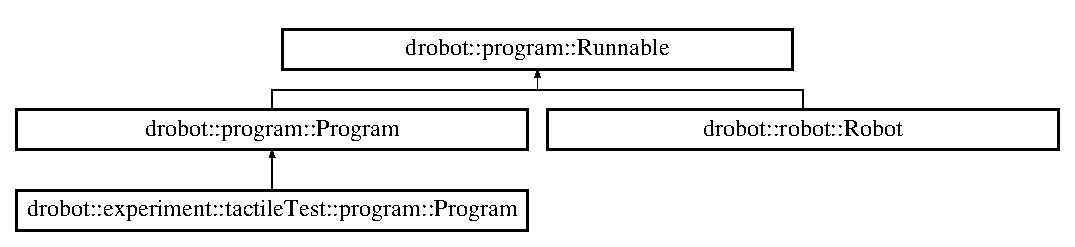
\includegraphics[height=2.876712cm]{classdrobot_1_1program_1_1Runnable}
\end{center}
\end{figure}
\subsection*{Public Member Functions}
\begin{DoxyCompactItemize}
\item 
\hypertarget{classdrobot_1_1program_1_1Runnable_afb99260eed1ee96fa96bf0a8ee03cfa5}{void \hyperlink{classdrobot_1_1program_1_1Runnable_afb99260eed1ee96fa96bf0a8ee03cfa5}{run\-\_\-thread} ()}\label{classdrobot_1_1program_1_1Runnable_afb99260eed1ee96fa96bf0a8ee03cfa5}

\begin{DoxyCompactList}\small\item\em run\-\_\-thread launches the run method in a new thread \end{DoxyCompactList}\item 
void \hyperlink{classdrobot_1_1program_1_1Runnable_ab453a9fcd85639e3c14f210e54d050b7}{run\-\_\-interval} (int msec)
\begin{DoxyCompactList}\small\item\em run\-\_\-interval repeatedly runs the run method in a specific interval \end{DoxyCompactList}\item 
\hypertarget{classdrobot_1_1program_1_1Runnable_a38595b3d0b4bf3c9ebcceb3dd6e5fdcc}{void \hyperlink{classdrobot_1_1program_1_1Runnable_a38595b3d0b4bf3c9ebcceb3dd6e5fdcc}{cancel} ()}\label{classdrobot_1_1program_1_1Runnable_a38595b3d0b4bf3c9ebcceb3dd6e5fdcc}

\begin{DoxyCompactList}\small\item\em cancel sets changes the \hyperlink{classdrobot_1_1program_1_1Runnable_ab22aef578839f56051702094b6f768df}{is\-Running()} method to return false \end{DoxyCompactList}\item 
bool \hyperlink{classdrobot_1_1program_1_1Runnable_ab22aef578839f56051702094b6f768df}{is\-Running} ()
\begin{DoxyCompactList}\small\item\em is\-Running returns true if the program is running. False otherwhise \end{DoxyCompactList}\item 
\hypertarget{classdrobot_1_1program_1_1Runnable_abbfe663f564dcfb5cfa157f59a56ed0d}{virtual void \hyperlink{classdrobot_1_1program_1_1Runnable_abbfe663f564dcfb5cfa157f59a56ed0d}{run} ()=0}\label{classdrobot_1_1program_1_1Runnable_abbfe663f564dcfb5cfa157f59a56ed0d}

\begin{DoxyCompactList}\small\item\em run has to be implemented by the child class. It should periodically check if \hyperlink{classdrobot_1_1program_1_1Runnable_ab22aef578839f56051702094b6f768df}{is\-Running()} still returns true. If it returns false the program should abort. \end{DoxyCompactList}\end{DoxyCompactItemize}
\subsection*{Protected Attributes}
\begin{DoxyCompactItemize}
\item 
\hypertarget{classdrobot_1_1program_1_1Runnable_acaf9a8bdc71804573fbae27ea6a603cd}{bool {\bfseries \-\_\-running}}\label{classdrobot_1_1program_1_1Runnable_acaf9a8bdc71804573fbae27ea6a603cd}

\end{DoxyCompactItemize}
\subsection*{Private Member Functions}
\begin{DoxyCompactItemize}
\item 
\hypertarget{classdrobot_1_1program_1_1Runnable_a83a6ffd50e6bd4cb2c8eae04b9df46b0}{void {\bfseries run\-\_\-interval\-\_\-loop} (int msec)}\label{classdrobot_1_1program_1_1Runnable_a83a6ffd50e6bd4cb2c8eae04b9df46b0}

\end{DoxyCompactItemize}


\subsection{Detailed Description}
base class for different kinds of threads. 

\subsection{Member Function Documentation}
\hypertarget{classdrobot_1_1program_1_1Runnable_ab22aef578839f56051702094b6f768df}{\index{drobot\-::program\-::\-Runnable@{drobot\-::program\-::\-Runnable}!is\-Running@{is\-Running}}
\index{is\-Running@{is\-Running}!drobot::program::Runnable@{drobot\-::program\-::\-Runnable}}
\subsubsection[{is\-Running}]{\setlength{\rightskip}{0pt plus 5cm}bool drobot\-::program\-::\-Runnable\-::is\-Running (
\begin{DoxyParamCaption}
{}
\end{DoxyParamCaption}
)}}\label{classdrobot_1_1program_1_1Runnable_ab22aef578839f56051702094b6f768df}


is\-Running returns true if the program is running. False otherwhise 

\begin{DoxyReturn}{Returns}
true if running, false otherwhise 
\end{DoxyReturn}
\hypertarget{classdrobot_1_1program_1_1Runnable_ab453a9fcd85639e3c14f210e54d050b7}{\index{drobot\-::program\-::\-Runnable@{drobot\-::program\-::\-Runnable}!run\-\_\-interval@{run\-\_\-interval}}
\index{run\-\_\-interval@{run\-\_\-interval}!drobot::program::Runnable@{drobot\-::program\-::\-Runnable}}
\subsubsection[{run\-\_\-interval}]{\setlength{\rightskip}{0pt plus 5cm}void drobot\-::program\-::\-Runnable\-::run\-\_\-interval (
\begin{DoxyParamCaption}
\item[{int}]{msec}
\end{DoxyParamCaption}
)}}\label{classdrobot_1_1program_1_1Runnable_ab453a9fcd85639e3c14f210e54d050b7}


run\-\_\-interval repeatedly runs the run method in a specific interval 


\begin{DoxyParams}{Parameters}
{\em msec} & \\
\hline
\end{DoxyParams}


The documentation for this class was generated from the following files\-:\begin{DoxyCompactItemize}
\item 
/home/imanol/workspace/drobot/new/src/drobot/program/runnable.\-h\item 
/home/imanol/workspace/drobot/new/src/drobot/program/runnable.\-cpp\end{DoxyCompactItemize}

\hypertarget{structdrobot_1_1datalogger_1_1SimpleDataLogEntry}{\section{drobot\-:\-:datalogger\-:\-:Simple\-Data\-Log\-Entry Struct Reference}
\label{structdrobot_1_1datalogger_1_1SimpleDataLogEntry}\index{drobot\-::datalogger\-::\-Simple\-Data\-Log\-Entry@{drobot\-::datalogger\-::\-Simple\-Data\-Log\-Entry}}
}


The \hyperlink{structdrobot_1_1datalogger_1_1SimpleDataLogEntry}{Simple\-Data\-Log\-Entry} struct contains the information about the channel values of one tick.  




{\ttfamily \#include $<$simpledatalogentry.\-h$>$}

\subsection*{Public Member Functions}
\begin{DoxyCompactItemize}
\item 
\hypertarget{structdrobot_1_1datalogger_1_1SimpleDataLogEntry_ac325c619e0e882fd0079a8239c5008e3}{{\bfseries Simple\-Data\-Log\-Entry} (long tick, std\-::map$<$ \hyperlink{classdrobot_1_1device_1_1channel_1_1Channel}{device\-::channel\-::\-Channel} $\ast$, double $>$ values)}\label{structdrobot_1_1datalogger_1_1SimpleDataLogEntry_ac325c619e0e882fd0079a8239c5008e3}

\end{DoxyCompactItemize}
\subsection*{Public Attributes}
\begin{DoxyCompactItemize}
\item 
\hypertarget{structdrobot_1_1datalogger_1_1SimpleDataLogEntry_a62f1b2c6b5e5a0ff20ed0e114fdad05b}{long {\bfseries tick}}\label{structdrobot_1_1datalogger_1_1SimpleDataLogEntry_a62f1b2c6b5e5a0ff20ed0e114fdad05b}

\item 
\hypertarget{structdrobot_1_1datalogger_1_1SimpleDataLogEntry_ad1602a5bcaf5fb0f61e27fb3e13f6a6d}{std\-::map\\*
$<$ \hyperlink{classdrobot_1_1device_1_1channel_1_1Channel}{device\-::channel\-::\-Channel} \\*
$\ast$, double $>$ {\bfseries values}}\label{structdrobot_1_1datalogger_1_1SimpleDataLogEntry_ad1602a5bcaf5fb0f61e27fb3e13f6a6d}

\end{DoxyCompactItemize}


\subsection{Detailed Description}
The \hyperlink{structdrobot_1_1datalogger_1_1SimpleDataLogEntry}{Simple\-Data\-Log\-Entry} struct contains the information about the channel values of one tick. 

The documentation for this struct was generated from the following file\-:\begin{DoxyCompactItemize}
\item 
/home/imanol/workspace/drobot/new/src/drobot/datalogger/simpledatalogentry.\-h\end{DoxyCompactItemize}

\hypertarget{classdrobot_1_1datalogger_1_1SimpleDataLogger}{\section{drobot\-:\-:datalogger\-:\-:Simple\-Data\-Logger Class Reference}
\label{classdrobot_1_1datalogger_1_1SimpleDataLogger}\index{drobot\-::datalogger\-::\-Simple\-Data\-Logger@{drobot\-::datalogger\-::\-Simple\-Data\-Logger}}
}


The \hyperlink{classdrobot_1_1datalogger_1_1SimpleDataLogger}{Simple\-Data\-Logger} class implements the \hyperlink{classdrobot_1_1datalogger_1_1DataLogger}{Data\-Logger} class to save it into a file and also load it from there.  




{\ttfamily \#include $<$simpledatalogger.\-h$>$}

Inheritance diagram for drobot\-:\-:datalogger\-:\-:Simple\-Data\-Logger\-:\begin{figure}[H]
\begin{center}
\leavevmode
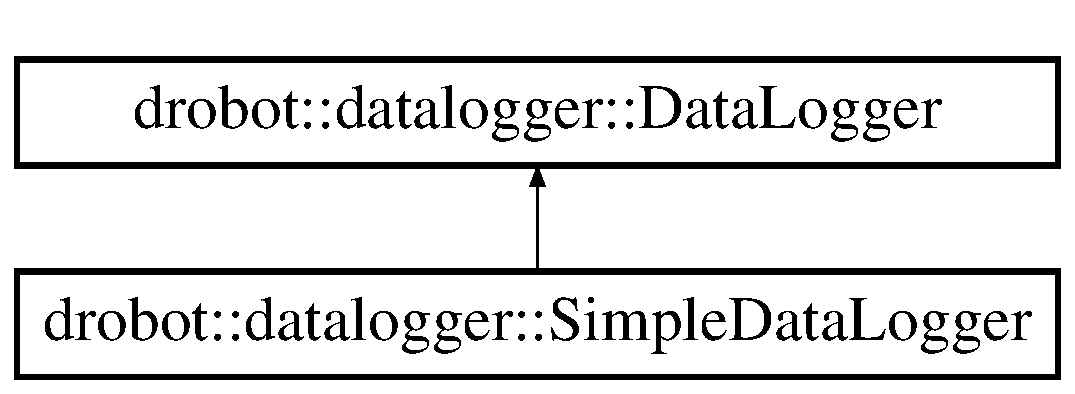
\includegraphics[height=3.000000cm]{classdrobot_1_1datalogger_1_1SimpleDataLogger}
\end{center}
\end{figure}
\subsection*{Public Member Functions}
\begin{DoxyCompactItemize}
\item 
\hypertarget{classdrobot_1_1datalogger_1_1SimpleDataLogger_a71822d737ffde7309da5b18a0eb71e3c}{{\bfseries Simple\-Data\-Logger} (int max\-Values, int modulo)}\label{classdrobot_1_1datalogger_1_1SimpleDataLogger_a71822d737ffde7309da5b18a0eb71e3c}

\item 
\hypertarget{classdrobot_1_1datalogger_1_1SimpleDataLogger_a46f2d6161b81c808fb6b6c6c75b457fc}{virtual void {\bfseries log} (long tick, std\-::map$<$ \hyperlink{classdrobot_1_1device_1_1channel_1_1Channel}{device\-::channel\-::\-Channel} $\ast$, double $>$ values)}\label{classdrobot_1_1datalogger_1_1SimpleDataLogger_a46f2d6161b81c808fb6b6c6c75b457fc}

\item 
virtual void \hyperlink{classdrobot_1_1datalogger_1_1SimpleDataLogger_a8e79821846b2104d7f65e64f6e8a5eb6}{set\-Max\-Values} (int max\-Values)
\begin{DoxyCompactList}\small\item\em set\-Max\-Values. max count of values. \end{DoxyCompactList}\item 
virtual int \hyperlink{classdrobot_1_1datalogger_1_1SimpleDataLogger_a2b9a75d2f73bb22e6558166e9dbcc4f4}{get\-Max\-Values} ()
\begin{DoxyCompactList}\small\item\em get\-Max\-Values. max count of values. \end{DoxyCompactList}\item 
virtual void \hyperlink{classdrobot_1_1datalogger_1_1SimpleDataLogger_a4365669efc4d0950cf21c30be8650a88}{set\-Modulo} (int modulo)
\begin{DoxyCompactList}\small\item\em set\-Modulo. which ticks are recorded \end{DoxyCompactList}\item 
virtual int \hyperlink{classdrobot_1_1datalogger_1_1SimpleDataLogger_a43d243494d611d7f1c6afd5204686f40}{get\-Modulo} ()
\begin{DoxyCompactList}\small\item\em get\-Modulo. which ticks are recorded \end{DoxyCompactList}\item 
\hypertarget{classdrobot_1_1datalogger_1_1SimpleDataLogger_a37c5777c063826a05d6242c61fc454cf}{void {\bfseries save\-To\-File} (std\-::string path)}\label{classdrobot_1_1datalogger_1_1SimpleDataLogger_a37c5777c063826a05d6242c61fc454cf}

\item 
\hypertarget{classdrobot_1_1datalogger_1_1SimpleDataLogger_ae99d6654f53748fbf22835f75bca978f}{void {\bfseries load\-From\-File} (std\-::string path, \hyperlink{classdrobot_1_1device_1_1channel_1_1ChannelManager}{device\-::channel\-::\-Channel\-Manager} channels)}\label{classdrobot_1_1datalogger_1_1SimpleDataLogger_ae99d6654f53748fbf22835f75bca978f}

\item 
\hypertarget{classdrobot_1_1datalogger_1_1SimpleDataLogger_a9a22c15bff8f3faaaed8ebe32f95d4d1}{std\-::vector$<$ \hyperlink{structdrobot_1_1datalogger_1_1SimpleDataLogEntry}{Simple\-Data\-Log\-Entry} $\ast$ $>$ {\bfseries get\-Data} ()}\label{classdrobot_1_1datalogger_1_1SimpleDataLogger_a9a22c15bff8f3faaaed8ebe32f95d4d1}

\end{DoxyCompactItemize}
\subsection*{Private Attributes}
\begin{DoxyCompactItemize}
\item 
\hypertarget{classdrobot_1_1datalogger_1_1SimpleDataLogger_a3163664f8050b0a428f61c4c8849cb15}{std\-::vector$<$ \hyperlink{structdrobot_1_1datalogger_1_1SimpleDataLogEntry}{Simple\-Data\-Log\-Entry} $\ast$ $>$ {\bfseries \-\_\-data}}\label{classdrobot_1_1datalogger_1_1SimpleDataLogger_a3163664f8050b0a428f61c4c8849cb15}

\item 
\hypertarget{classdrobot_1_1datalogger_1_1SimpleDataLogger_af2603933a4ed7fb1231896fbee220752}{int {\bfseries \-\_\-modulo}}\label{classdrobot_1_1datalogger_1_1SimpleDataLogger_af2603933a4ed7fb1231896fbee220752}

\item 
\hypertarget{classdrobot_1_1datalogger_1_1SimpleDataLogger_afb8dceee27c888b76b5eec720f3cff3b}{int {\bfseries \-\_\-max\-Values}}\label{classdrobot_1_1datalogger_1_1SimpleDataLogger_afb8dceee27c888b76b5eec720f3cff3b}

\end{DoxyCompactItemize}
\subsection*{Additional Inherited Members}


\subsection{Detailed Description}
The \hyperlink{classdrobot_1_1datalogger_1_1SimpleDataLogger}{Simple\-Data\-Logger} class implements the \hyperlink{classdrobot_1_1datalogger_1_1DataLogger}{Data\-Logger} class to save it into a file and also load it from there. 

\subsection{Member Function Documentation}
\hypertarget{classdrobot_1_1datalogger_1_1SimpleDataLogger_a2b9a75d2f73bb22e6558166e9dbcc4f4}{\index{drobot\-::datalogger\-::\-Simple\-Data\-Logger@{drobot\-::datalogger\-::\-Simple\-Data\-Logger}!get\-Max\-Values@{get\-Max\-Values}}
\index{get\-Max\-Values@{get\-Max\-Values}!drobot::datalogger::SimpleDataLogger@{drobot\-::datalogger\-::\-Simple\-Data\-Logger}}
\subsubsection[{get\-Max\-Values}]{\setlength{\rightskip}{0pt plus 5cm}int drobot\-::datalogger\-::\-Simple\-Data\-Logger\-::get\-Max\-Values (
\begin{DoxyParamCaption}
{}
\end{DoxyParamCaption}
)\hspace{0.3cm}{\ttfamily [virtual]}}}\label{classdrobot_1_1datalogger_1_1SimpleDataLogger_a2b9a75d2f73bb22e6558166e9dbcc4f4}


get\-Max\-Values. max count of values. 

If bigger than 0 the values from the oldest ticks are deleted so that the size doesn't exceeds max\-Values \begin{DoxyReturn}{Returns}
max\-Values 
\end{DoxyReturn}


Implements \hyperlink{classdrobot_1_1datalogger_1_1DataLogger_a8fe7bb2a626d9f9d5c69f9197490515b}{drobot\-::datalogger\-::\-Data\-Logger}.

\hypertarget{classdrobot_1_1datalogger_1_1SimpleDataLogger_a43d243494d611d7f1c6afd5204686f40}{\index{drobot\-::datalogger\-::\-Simple\-Data\-Logger@{drobot\-::datalogger\-::\-Simple\-Data\-Logger}!get\-Modulo@{get\-Modulo}}
\index{get\-Modulo@{get\-Modulo}!drobot::datalogger::SimpleDataLogger@{drobot\-::datalogger\-::\-Simple\-Data\-Logger}}
\subsubsection[{get\-Modulo}]{\setlength{\rightskip}{0pt plus 5cm}int drobot\-::datalogger\-::\-Simple\-Data\-Logger\-::get\-Modulo (
\begin{DoxyParamCaption}
{}
\end{DoxyParamCaption}
)\hspace{0.3cm}{\ttfamily [virtual]}}}\label{classdrobot_1_1datalogger_1_1SimpleDataLogger_a43d243494d611d7f1c6afd5204686f40}


get\-Modulo. which ticks are recorded 

if bigger than 0 only ticks with (tick \% module == 0) are recorded \begin{DoxyReturn}{Returns}
modulo 
\end{DoxyReturn}


Implements \hyperlink{classdrobot_1_1datalogger_1_1DataLogger_a4dd79d4060e4d4d77451a50777792c0a}{drobot\-::datalogger\-::\-Data\-Logger}.

\hypertarget{classdrobot_1_1datalogger_1_1SimpleDataLogger_a8e79821846b2104d7f65e64f6e8a5eb6}{\index{drobot\-::datalogger\-::\-Simple\-Data\-Logger@{drobot\-::datalogger\-::\-Simple\-Data\-Logger}!set\-Max\-Values@{set\-Max\-Values}}
\index{set\-Max\-Values@{set\-Max\-Values}!drobot::datalogger::SimpleDataLogger@{drobot\-::datalogger\-::\-Simple\-Data\-Logger}}
\subsubsection[{set\-Max\-Values}]{\setlength{\rightskip}{0pt plus 5cm}void drobot\-::datalogger\-::\-Simple\-Data\-Logger\-::set\-Max\-Values (
\begin{DoxyParamCaption}
\item[{int}]{max\-Values}
\end{DoxyParamCaption}
)\hspace{0.3cm}{\ttfamily [virtual]}}}\label{classdrobot_1_1datalogger_1_1SimpleDataLogger_a8e79821846b2104d7f65e64f6e8a5eb6}


set\-Max\-Values. max count of values. 

If bigger than 0 the values from the oldest ticks are deleted so that the size doesn't exceeds max\-Values 
\begin{DoxyParams}{Parameters}
{\em max\-Values} & \\
\hline
\end{DoxyParams}


Implements \hyperlink{classdrobot_1_1datalogger_1_1DataLogger_ae90262e477952f8e1c385b84e17d80c6}{drobot\-::datalogger\-::\-Data\-Logger}.

\hypertarget{classdrobot_1_1datalogger_1_1SimpleDataLogger_a4365669efc4d0950cf21c30be8650a88}{\index{drobot\-::datalogger\-::\-Simple\-Data\-Logger@{drobot\-::datalogger\-::\-Simple\-Data\-Logger}!set\-Modulo@{set\-Modulo}}
\index{set\-Modulo@{set\-Modulo}!drobot::datalogger::SimpleDataLogger@{drobot\-::datalogger\-::\-Simple\-Data\-Logger}}
\subsubsection[{set\-Modulo}]{\setlength{\rightskip}{0pt plus 5cm}void drobot\-::datalogger\-::\-Simple\-Data\-Logger\-::set\-Modulo (
\begin{DoxyParamCaption}
\item[{int}]{modulo}
\end{DoxyParamCaption}
)\hspace{0.3cm}{\ttfamily [virtual]}}}\label{classdrobot_1_1datalogger_1_1SimpleDataLogger_a4365669efc4d0950cf21c30be8650a88}


set\-Modulo. which ticks are recorded 

if bigger than 0 only ticks with (tick \% module == 0) are recorded 
\begin{DoxyParams}{Parameters}
{\em modulo} & \\
\hline
\end{DoxyParams}


Implements \hyperlink{classdrobot_1_1datalogger_1_1DataLogger_ae463aebd8cb38c716bef83d5732042b1}{drobot\-::datalogger\-::\-Data\-Logger}.



The documentation for this class was generated from the following files\-:\begin{DoxyCompactItemize}
\item 
/home/imanol/workspace/drobot/new/src/drobot/datalogger/simpledatalogger.\-h\item 
/home/imanol/workspace/drobot/new/src/drobot/datalogger/simpledatalogger.\-cpp\end{DoxyCompactItemize}

\hypertarget{classdrobot_1_1device_1_1tactile_1_1SimpleTactileSensor}{\section{drobot\-:\-:device\-:\-:tactile\-:\-:Simple\-Tactile\-Sensor Class Reference}
\label{classdrobot_1_1device_1_1tactile_1_1SimpleTactileSensor}\index{drobot\-::device\-::tactile\-::\-Simple\-Tactile\-Sensor@{drobot\-::device\-::tactile\-::\-Simple\-Tactile\-Sensor}}
}


The \hyperlink{classdrobot_1_1device_1_1tactile_1_1SimpleTactileSensor}{Simple\-Tactile\-Sensor} class represents a tactile sensor which is connected to a \hyperlink{classdrobot_1_1device_1_1tactile_1_1SimpleTactileSensorBoard}{Simple\-Tactile\-Sensor\-Board}.  




{\ttfamily \#include $<$simpletactilesensor.\-h$>$}

Inheritance diagram for drobot\-:\-:device\-:\-:tactile\-:\-:Simple\-Tactile\-Sensor\-:\begin{figure}[H]
\begin{center}
\leavevmode
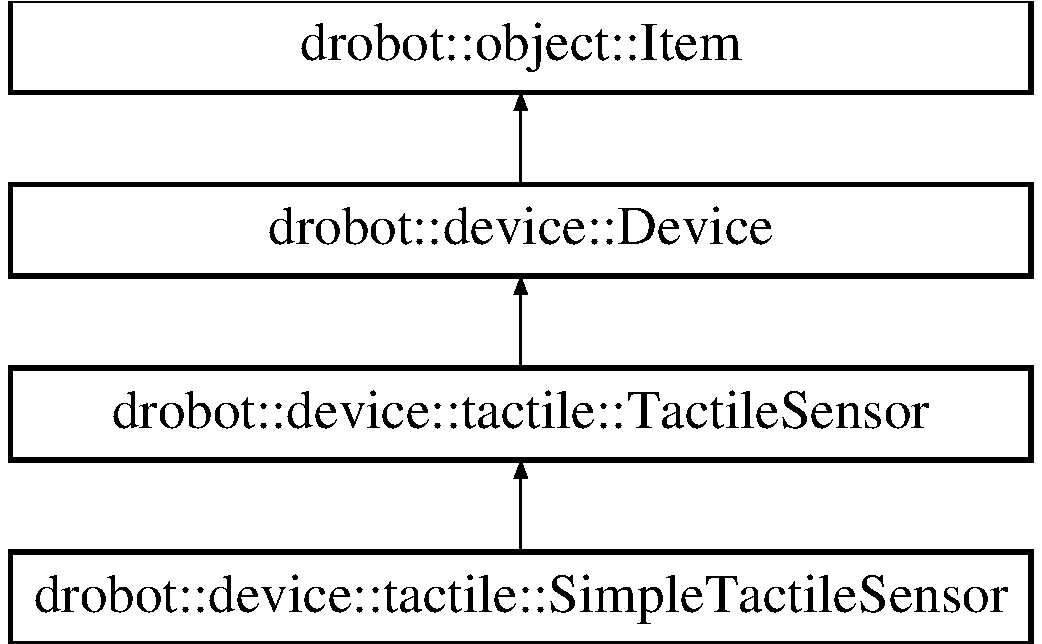
\includegraphics[height=4.000000cm]{classdrobot_1_1device_1_1tactile_1_1SimpleTactileSensor}
\end{center}
\end{figure}
\subsection*{Public Member Functions}
\begin{DoxyCompactItemize}
\item 
\hypertarget{classdrobot_1_1device_1_1tactile_1_1SimpleTactileSensor_acd670a819320a63177f9eb6f88691fc7}{{\bfseries Simple\-Tactile\-Sensor} (std\-::string name, int index)}\label{classdrobot_1_1device_1_1tactile_1_1SimpleTactileSensor_acd670a819320a63177f9eb6f88691fc7}

\item 
\hypertarget{classdrobot_1_1device_1_1tactile_1_1SimpleTactileSensor_a2e5d7cc36402602496016a302e8da363}{{\bfseries Simple\-Tactile\-Sensor} (std\-::string name, int index, double value)}\label{classdrobot_1_1device_1_1tactile_1_1SimpleTactileSensor_a2e5d7cc36402602496016a302e8da363}

\item 
int \hyperlink{classdrobot_1_1device_1_1tactile_1_1SimpleTactileSensor_a63ae2c9a6ec73bf35d23f6012365aecb}{get\-Index} ()
\item 
virtual double \hyperlink{classdrobot_1_1device_1_1tactile_1_1SimpleTactileSensor_a8f9d1aec99cd3c53bac343af3a3bda60}{get\-Value} ()
\item 
\hypertarget{classdrobot_1_1device_1_1tactile_1_1SimpleTactileSensor_a6c09c4748dfbacf9b62b1e2f811827c0}{void {\bfseries set\-Value} (double value)}\label{classdrobot_1_1device_1_1tactile_1_1SimpleTactileSensor_a6c09c4748dfbacf9b62b1e2f811827c0}

\item 
virtual double \hyperlink{classdrobot_1_1device_1_1tactile_1_1SimpleTactileSensor_aff61edb7f9ccdac4f0209590bb8d7d76}{get\-Value\-Min} ()
\item 
virtual double \hyperlink{classdrobot_1_1device_1_1tactile_1_1SimpleTactileSensor_aa5e6c1634c8fafe61e41cb998c02b6b6}{get\-Value\-Max} ()
\item 
virtual void \hyperlink{classdrobot_1_1device_1_1tactile_1_1SimpleTactileSensor_a006318b86b569b7f72605d24f1948042}{enable} ()
\begin{DoxyCompactList}\small\item\em enables the device. \end{DoxyCompactList}\item 
virtual void \hyperlink{classdrobot_1_1device_1_1tactile_1_1SimpleTactileSensor_a0599c06afdb09494de0e6756a878cbad}{disable} ()
\begin{DoxyCompactList}\small\item\em disables the device. \end{DoxyCompactList}\item 
virtual bool \hyperlink{classdrobot_1_1device_1_1tactile_1_1SimpleTactileSensor_a54b5ab7b69bb3b15727ef72143799f34}{is\-Enabled} ()
\begin{DoxyCompactList}\small\item\em check if the device is enabled \end{DoxyCompactList}\end{DoxyCompactItemize}
\subsection*{Private Attributes}
\begin{DoxyCompactItemize}
\item 
\hypertarget{classdrobot_1_1device_1_1tactile_1_1SimpleTactileSensor_a6bdcac9b1bc69f264bb0ae022c2f79d2}{double {\bfseries \-\_\-value}}\label{classdrobot_1_1device_1_1tactile_1_1SimpleTactileSensor_a6bdcac9b1bc69f264bb0ae022c2f79d2}

\item 
\hypertarget{classdrobot_1_1device_1_1tactile_1_1SimpleTactileSensor_a922f8bb56fda64b48ec90fbd9362f1da}{bool {\bfseries \-\_\-enabled}}\label{classdrobot_1_1device_1_1tactile_1_1SimpleTactileSensor_a922f8bb56fda64b48ec90fbd9362f1da}

\item 
\hypertarget{classdrobot_1_1device_1_1tactile_1_1SimpleTactileSensor_a787c9f35cd15b0ef485d3c6ca771241c}{int {\bfseries \-\_\-index}}\label{classdrobot_1_1device_1_1tactile_1_1SimpleTactileSensor_a787c9f35cd15b0ef485d3c6ca771241c}

\end{DoxyCompactItemize}
\subsection*{Additional Inherited Members}


\subsection{Detailed Description}
The \hyperlink{classdrobot_1_1device_1_1tactile_1_1SimpleTactileSensor}{Simple\-Tactile\-Sensor} class represents a tactile sensor which is connected to a \hyperlink{classdrobot_1_1device_1_1tactile_1_1SimpleTactileSensorBoard}{Simple\-Tactile\-Sensor\-Board}. 

\subsection{Member Function Documentation}
\hypertarget{classdrobot_1_1device_1_1tactile_1_1SimpleTactileSensor_a0599c06afdb09494de0e6756a878cbad}{\index{drobot\-::device\-::tactile\-::\-Simple\-Tactile\-Sensor@{drobot\-::device\-::tactile\-::\-Simple\-Tactile\-Sensor}!disable@{disable}}
\index{disable@{disable}!drobot::device::tactile::SimpleTactileSensor@{drobot\-::device\-::tactile\-::\-Simple\-Tactile\-Sensor}}
\subsubsection[{disable}]{\setlength{\rightskip}{0pt plus 5cm}void drobot\-::device\-::tactile\-::\-Simple\-Tactile\-Sensor\-::disable (
\begin{DoxyParamCaption}
{}
\end{DoxyParamCaption}
)\hspace{0.3cm}{\ttfamily [virtual]}}}\label{classdrobot_1_1device_1_1tactile_1_1SimpleTactileSensor_a0599c06afdb09494de0e6756a878cbad}


disables the device. 

This function has to be implemented by the specific device. For physical devices like actuators this method should power off the device; 

Reimplemented from \hyperlink{classdrobot_1_1device_1_1Device_a289499673ae30bd72101c68fbd04cd89}{drobot\-::device\-::\-Device}.

\hypertarget{classdrobot_1_1device_1_1tactile_1_1SimpleTactileSensor_a006318b86b569b7f72605d24f1948042}{\index{drobot\-::device\-::tactile\-::\-Simple\-Tactile\-Sensor@{drobot\-::device\-::tactile\-::\-Simple\-Tactile\-Sensor}!enable@{enable}}
\index{enable@{enable}!drobot::device::tactile::SimpleTactileSensor@{drobot\-::device\-::tactile\-::\-Simple\-Tactile\-Sensor}}
\subsubsection[{enable}]{\setlength{\rightskip}{0pt plus 5cm}void drobot\-::device\-::tactile\-::\-Simple\-Tactile\-Sensor\-::enable (
\begin{DoxyParamCaption}
{}
\end{DoxyParamCaption}
)\hspace{0.3cm}{\ttfamily [virtual]}}}\label{classdrobot_1_1device_1_1tactile_1_1SimpleTactileSensor_a006318b86b569b7f72605d24f1948042}


enables the device. 

This function has to be implemented by the specific device. For physical devices like actuators this method should power on the device. 

Reimplemented from \hyperlink{classdrobot_1_1device_1_1Device_a0c28785ff2e79f99b8e9eaefe6749f2b}{drobot\-::device\-::\-Device}.

\hypertarget{classdrobot_1_1device_1_1tactile_1_1SimpleTactileSensor_a63ae2c9a6ec73bf35d23f6012365aecb}{\index{drobot\-::device\-::tactile\-::\-Simple\-Tactile\-Sensor@{drobot\-::device\-::tactile\-::\-Simple\-Tactile\-Sensor}!get\-Index@{get\-Index}}
\index{get\-Index@{get\-Index}!drobot::device::tactile::SimpleTactileSensor@{drobot\-::device\-::tactile\-::\-Simple\-Tactile\-Sensor}}
\subsubsection[{get\-Index}]{\setlength{\rightskip}{0pt plus 5cm}int drobot\-::device\-::tactile\-::\-Simple\-Tactile\-Sensor\-::get\-Index (
\begin{DoxyParamCaption}
{}
\end{DoxyParamCaption}
)}}\label{classdrobot_1_1device_1_1tactile_1_1SimpleTactileSensor_a63ae2c9a6ec73bf35d23f6012365aecb}
\begin{DoxyReturn}{Returns}
index of the slot the sensor is plugged into the sensor board 
\end{DoxyReturn}
\hypertarget{classdrobot_1_1device_1_1tactile_1_1SimpleTactileSensor_a8f9d1aec99cd3c53bac343af3a3bda60}{\index{drobot\-::device\-::tactile\-::\-Simple\-Tactile\-Sensor@{drobot\-::device\-::tactile\-::\-Simple\-Tactile\-Sensor}!get\-Value@{get\-Value}}
\index{get\-Value@{get\-Value}!drobot::device::tactile::SimpleTactileSensor@{drobot\-::device\-::tactile\-::\-Simple\-Tactile\-Sensor}}
\subsubsection[{get\-Value}]{\setlength{\rightskip}{0pt plus 5cm}double drobot\-::device\-::tactile\-::\-Simple\-Tactile\-Sensor\-::get\-Value (
\begin{DoxyParamCaption}
{}
\end{DoxyParamCaption}
)\hspace{0.3cm}{\ttfamily [virtual]}}}\label{classdrobot_1_1device_1_1tactile_1_1SimpleTactileSensor_a8f9d1aec99cd3c53bac343af3a3bda60}
\begin{DoxyReturn}{Returns}
current value of the tactile sensor 
\end{DoxyReturn}


Implements \hyperlink{classdrobot_1_1device_1_1tactile_1_1TactileSensor_a89fd3eb13e03638fba38fa6a4b8d17ed}{drobot\-::device\-::tactile\-::\-Tactile\-Sensor}.

\hypertarget{classdrobot_1_1device_1_1tactile_1_1SimpleTactileSensor_aa5e6c1634c8fafe61e41cb998c02b6b6}{\index{drobot\-::device\-::tactile\-::\-Simple\-Tactile\-Sensor@{drobot\-::device\-::tactile\-::\-Simple\-Tactile\-Sensor}!get\-Value\-Max@{get\-Value\-Max}}
\index{get\-Value\-Max@{get\-Value\-Max}!drobot::device::tactile::SimpleTactileSensor@{drobot\-::device\-::tactile\-::\-Simple\-Tactile\-Sensor}}
\subsubsection[{get\-Value\-Max}]{\setlength{\rightskip}{0pt plus 5cm}double drobot\-::device\-::tactile\-::\-Simple\-Tactile\-Sensor\-::get\-Value\-Max (
\begin{DoxyParamCaption}
{}
\end{DoxyParamCaption}
)\hspace{0.3cm}{\ttfamily [virtual]}}}\label{classdrobot_1_1device_1_1tactile_1_1SimpleTactileSensor_aa5e6c1634c8fafe61e41cb998c02b6b6}
\begin{DoxyReturn}{Returns}
maximal possible value 
\end{DoxyReturn}


Implements \hyperlink{classdrobot_1_1device_1_1tactile_1_1TactileSensor_a03eb99ccdc4bb78818ce556c440d372a}{drobot\-::device\-::tactile\-::\-Tactile\-Sensor}.

\hypertarget{classdrobot_1_1device_1_1tactile_1_1SimpleTactileSensor_aff61edb7f9ccdac4f0209590bb8d7d76}{\index{drobot\-::device\-::tactile\-::\-Simple\-Tactile\-Sensor@{drobot\-::device\-::tactile\-::\-Simple\-Tactile\-Sensor}!get\-Value\-Min@{get\-Value\-Min}}
\index{get\-Value\-Min@{get\-Value\-Min}!drobot::device::tactile::SimpleTactileSensor@{drobot\-::device\-::tactile\-::\-Simple\-Tactile\-Sensor}}
\subsubsection[{get\-Value\-Min}]{\setlength{\rightskip}{0pt plus 5cm}double drobot\-::device\-::tactile\-::\-Simple\-Tactile\-Sensor\-::get\-Value\-Min (
\begin{DoxyParamCaption}
{}
\end{DoxyParamCaption}
)\hspace{0.3cm}{\ttfamily [virtual]}}}\label{classdrobot_1_1device_1_1tactile_1_1SimpleTactileSensor_aff61edb7f9ccdac4f0209590bb8d7d76}
\begin{DoxyReturn}{Returns}
minimal possible value 
\end{DoxyReturn}


Implements \hyperlink{classdrobot_1_1device_1_1tactile_1_1TactileSensor_ae586a70280096eb764188a94c9044470}{drobot\-::device\-::tactile\-::\-Tactile\-Sensor}.

\hypertarget{classdrobot_1_1device_1_1tactile_1_1SimpleTactileSensor_a54b5ab7b69bb3b15727ef72143799f34}{\index{drobot\-::device\-::tactile\-::\-Simple\-Tactile\-Sensor@{drobot\-::device\-::tactile\-::\-Simple\-Tactile\-Sensor}!is\-Enabled@{is\-Enabled}}
\index{is\-Enabled@{is\-Enabled}!drobot::device::tactile::SimpleTactileSensor@{drobot\-::device\-::tactile\-::\-Simple\-Tactile\-Sensor}}
\subsubsection[{is\-Enabled}]{\setlength{\rightskip}{0pt plus 5cm}bool drobot\-::device\-::tactile\-::\-Simple\-Tactile\-Sensor\-::is\-Enabled (
\begin{DoxyParamCaption}
{}
\end{DoxyParamCaption}
)\hspace{0.3cm}{\ttfamily [virtual]}}}\label{classdrobot_1_1device_1_1tactile_1_1SimpleTactileSensor_a54b5ab7b69bb3b15727ef72143799f34}


check if the device is enabled 

\begin{DoxyReturn}{Returns}
true if enabled else false
\end{DoxyReturn}
While the \hyperlink{classdrobot_1_1robot_1_1Robot}{drobot\-::robot\-::\-Robot} is running this property is checked to see whether the device should be used or not. 

Implements \hyperlink{classdrobot_1_1device_1_1Device_aa5b7eac8638d0d2d5ee9bf10607b100e}{drobot\-::device\-::\-Device}.



The documentation for this class was generated from the following files\-:\begin{DoxyCompactItemize}
\item 
src/drobot/device/tactile/simpletactilesensor.\-h\item 
src/drobot/device/tactile/simpletactilesensor.\-cpp\end{DoxyCompactItemize}

\hypertarget{classdrobot_1_1device_1_1tactile_1_1SimpleTactileSensorBoard}{\section{drobot\-:\-:device\-:\-:tactile\-:\-:Simple\-Tactile\-Sensor\-Board Class Reference}
\label{classdrobot_1_1device_1_1tactile_1_1SimpleTactileSensorBoard}\index{drobot\-::device\-::tactile\-::\-Simple\-Tactile\-Sensor\-Board@{drobot\-::device\-::tactile\-::\-Simple\-Tactile\-Sensor\-Board}}
}


The \hyperlink{classdrobot_1_1device_1_1tactile_1_1SimpleTactileSensorBoard}{Simple\-Tactile\-Sensor\-Board} class.  




{\ttfamily \#include $<$simpletactilesensorboard.\-h$>$}

Inheritance diagram for drobot\-:\-:device\-:\-:tactile\-:\-:Simple\-Tactile\-Sensor\-Board\-:\begin{figure}[H]
\begin{center}
\leavevmode
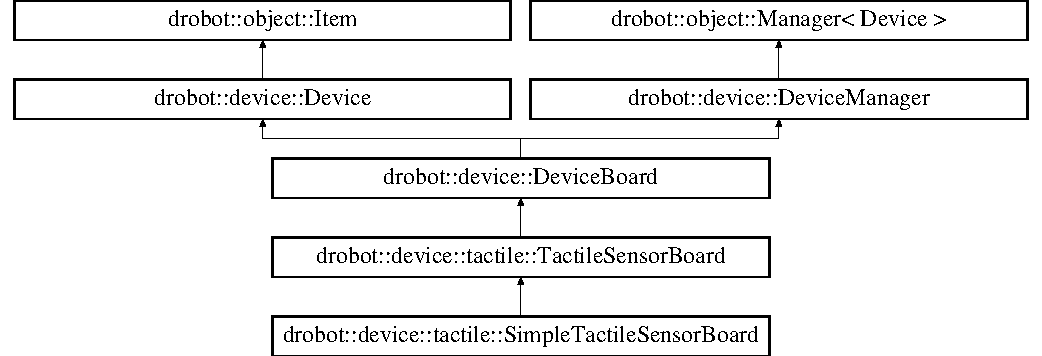
\includegraphics[height=4.778157cm]{classdrobot_1_1device_1_1tactile_1_1SimpleTactileSensorBoard}
\end{center}
\end{figure}
\subsection*{Public Member Functions}
\begin{DoxyCompactItemize}
\item 
\hypertarget{classdrobot_1_1device_1_1tactile_1_1SimpleTactileSensorBoard_a22778b1f5cdba96f49875a0e92c6e2f7}{{\bfseries Simple\-Tactile\-Sensor\-Board} (std\-::string name, std\-::string path)}\label{classdrobot_1_1device_1_1tactile_1_1SimpleTactileSensorBoard_a22778b1f5cdba96f49875a0e92c6e2f7}

\item 
\hypertarget{classdrobot_1_1device_1_1tactile_1_1SimpleTactileSensorBoard_a3e1d250aaa890d6e35ae1dd79397216c}{{\bfseries Simple\-Tactile\-Sensor\-Board} (std\-::string name, std\-::string path, int max\-Sensors)}\label{classdrobot_1_1device_1_1tactile_1_1SimpleTactileSensorBoard_a3e1d250aaa890d6e35ae1dd79397216c}

\item 
virtual void \hyperlink{classdrobot_1_1device_1_1tactile_1_1SimpleTactileSensorBoard_a1660e1e8cd1d5705936a28ce9294d759}{enable} ()
\begin{DoxyCompactList}\small\item\em enables the device. \end{DoxyCompactList}\item 
void \hyperlink{classdrobot_1_1device_1_1tactile_1_1SimpleTactileSensorBoard_aa857348183ae4940a545fc67440129ce}{update\-Loop} ()
\begin{DoxyCompactList}\small\item\em updates the values of the Simple\-Tactile\-Sensors in a loop. \end{DoxyCompactList}\item 
std\-::vector$<$ \hyperlink{classdrobot_1_1device_1_1tactile_1_1TactileSensor}{Tactile\-Sensor} $\ast$ $>$ \hyperlink{classdrobot_1_1device_1_1tactile_1_1SimpleTactileSensorBoard_ac2097d7088c8b86f1597d5dcc1a7f447}{init\-All\-Sensors} ()
\begin{DoxyCompactList}\small\item\em initializes all the sensors and adds them to the board \end{DoxyCompactList}\item 
\hyperlink{classdrobot_1_1device_1_1tactile_1_1TactileSensor}{Tactile\-Sensor} $\ast$ \hyperlink{classdrobot_1_1device_1_1tactile_1_1SimpleTactileSensorBoard_a1469177db6d4de1c320bd24cc7750d65}{init\-Sensor} (int index, std\-::string name)
\begin{DoxyCompactList}\small\item\em initializes a sensor at the given index and adds them to the board \end{DoxyCompactList}\item 
\hyperlink{classdrobot_1_1device_1_1tactile_1_1TactileSensor}{Tactile\-Sensor} $\ast$ \hyperlink{classdrobot_1_1device_1_1tactile_1_1SimpleTactileSensorBoard_a2c793a9f64826941dd58dc2ddcbd3283}{init\-Sensor} (int index)
\begin{DoxyCompactList}\small\item\em initializes a sensor at the given index and adds it to the board \end{DoxyCompactList}\item 
\hypertarget{classdrobot_1_1device_1_1tactile_1_1SimpleTactileSensorBoard_a978ec8471e2589de983e9b1195dcc9ed}{\hyperlink{classdrobot_1_1device_1_1tactile_1_1SimpleTactileSensor}{Simple\-Tactile\-Sensor} $\ast$ {\bfseries get\-Tactile\-Sensor} (int index)}\label{classdrobot_1_1device_1_1tactile_1_1SimpleTactileSensorBoard_a978ec8471e2589de983e9b1195dcc9ed}

\end{DoxyCompactItemize}
\subsection*{Private Attributes}
\begin{DoxyCompactItemize}
\item 
\hypertarget{classdrobot_1_1device_1_1tactile_1_1SimpleTactileSensorBoard_a0242cf52a0f5d10cb176bb269aa57f95}{std\-::string {\bfseries \-\_\-path}}\label{classdrobot_1_1device_1_1tactile_1_1SimpleTactileSensorBoard_a0242cf52a0f5d10cb176bb269aa57f95}

\item 
\hypertarget{classdrobot_1_1device_1_1tactile_1_1SimpleTactileSensorBoard_ad12ae05c2b620e2809fac3191d6e2198}{int {\bfseries \-\_\-max\-Sensors}}\label{classdrobot_1_1device_1_1tactile_1_1SimpleTactileSensorBoard_ad12ae05c2b620e2809fac3191d6e2198}

\end{DoxyCompactItemize}
\subsection*{Additional Inherited Members}


\subsection{Detailed Description}
The \hyperlink{classdrobot_1_1device_1_1tactile_1_1SimpleTactileSensorBoard}{Simple\-Tactile\-Sensor\-Board} class. 

\subsection{Member Function Documentation}
\hypertarget{classdrobot_1_1device_1_1tactile_1_1SimpleTactileSensorBoard_a1660e1e8cd1d5705936a28ce9294d759}{\index{drobot\-::device\-::tactile\-::\-Simple\-Tactile\-Sensor\-Board@{drobot\-::device\-::tactile\-::\-Simple\-Tactile\-Sensor\-Board}!enable@{enable}}
\index{enable@{enable}!drobot::device::tactile::SimpleTactileSensorBoard@{drobot\-::device\-::tactile\-::\-Simple\-Tactile\-Sensor\-Board}}
\subsubsection[{enable}]{\setlength{\rightskip}{0pt plus 5cm}void drobot\-::device\-::tactile\-::\-Simple\-Tactile\-Sensor\-Board\-::enable (
\begin{DoxyParamCaption}
{}
\end{DoxyParamCaption}
)\hspace{0.3cm}{\ttfamily [virtual]}}}\label{classdrobot_1_1device_1_1tactile_1_1SimpleTactileSensorBoard_a1660e1e8cd1d5705936a28ce9294d759}


enables the device. 

This function has to be implemented by the specific device. For physical devices like actuators this method should power on the device. 

Reimplemented from \hyperlink{classdrobot_1_1device_1_1DeviceBoard_a1a01810b04372666baaafaf812e5a54e}{drobot\-::device\-::\-Device\-Board}.

\hypertarget{classdrobot_1_1device_1_1tactile_1_1SimpleTactileSensorBoard_ac2097d7088c8b86f1597d5dcc1a7f447}{\index{drobot\-::device\-::tactile\-::\-Simple\-Tactile\-Sensor\-Board@{drobot\-::device\-::tactile\-::\-Simple\-Tactile\-Sensor\-Board}!init\-All\-Sensors@{init\-All\-Sensors}}
\index{init\-All\-Sensors@{init\-All\-Sensors}!drobot::device::tactile::SimpleTactileSensorBoard@{drobot\-::device\-::tactile\-::\-Simple\-Tactile\-Sensor\-Board}}
\subsubsection[{init\-All\-Sensors}]{\setlength{\rightskip}{0pt plus 5cm}std\-::vector$<$ {\bf Tactile\-Sensor} $\ast$ $>$ drobot\-::device\-::tactile\-::\-Simple\-Tactile\-Sensor\-Board\-::init\-All\-Sensors (
\begin{DoxyParamCaption}
{}
\end{DoxyParamCaption}
)}}\label{classdrobot_1_1device_1_1tactile_1_1SimpleTactileSensorBoard_ac2097d7088c8b86f1597d5dcc1a7f447}


initializes all the sensors and adds them to the board 

\begin{DoxyReturn}{Returns}
initialized sensors 
\end{DoxyReturn}
\hypertarget{classdrobot_1_1device_1_1tactile_1_1SimpleTactileSensorBoard_a1469177db6d4de1c320bd24cc7750d65}{\index{drobot\-::device\-::tactile\-::\-Simple\-Tactile\-Sensor\-Board@{drobot\-::device\-::tactile\-::\-Simple\-Tactile\-Sensor\-Board}!init\-Sensor@{init\-Sensor}}
\index{init\-Sensor@{init\-Sensor}!drobot::device::tactile::SimpleTactileSensorBoard@{drobot\-::device\-::tactile\-::\-Simple\-Tactile\-Sensor\-Board}}
\subsubsection[{init\-Sensor}]{\setlength{\rightskip}{0pt plus 5cm}{\bf Tactile\-Sensor} $\ast$ drobot\-::device\-::tactile\-::\-Simple\-Tactile\-Sensor\-Board\-::init\-Sensor (
\begin{DoxyParamCaption}
\item[{int}]{index, }
\item[{std\-::string}]{name}
\end{DoxyParamCaption}
)}}\label{classdrobot_1_1device_1_1tactile_1_1SimpleTactileSensorBoard_a1469177db6d4de1c320bd24cc7750d65}


initializes a sensor at the given index and adds them to the board 


\begin{DoxyParams}{Parameters}
{\em index} & \\
\hline
{\em name} & \\
\hline
\end{DoxyParams}
\begin{DoxyReturn}{Returns}
initialized sensor 
\end{DoxyReturn}
\hypertarget{classdrobot_1_1device_1_1tactile_1_1SimpleTactileSensorBoard_a2c793a9f64826941dd58dc2ddcbd3283}{\index{drobot\-::device\-::tactile\-::\-Simple\-Tactile\-Sensor\-Board@{drobot\-::device\-::tactile\-::\-Simple\-Tactile\-Sensor\-Board}!init\-Sensor@{init\-Sensor}}
\index{init\-Sensor@{init\-Sensor}!drobot::device::tactile::SimpleTactileSensorBoard@{drobot\-::device\-::tactile\-::\-Simple\-Tactile\-Sensor\-Board}}
\subsubsection[{init\-Sensor}]{\setlength{\rightskip}{0pt plus 5cm}{\bf Tactile\-Sensor} $\ast$ drobot\-::device\-::tactile\-::\-Simple\-Tactile\-Sensor\-Board\-::init\-Sensor (
\begin{DoxyParamCaption}
\item[{int}]{index}
\end{DoxyParamCaption}
)}}\label{classdrobot_1_1device_1_1tactile_1_1SimpleTactileSensorBoard_a2c793a9f64826941dd58dc2ddcbd3283}


initializes a sensor at the given index and adds it to the board 


\begin{DoxyParams}{Parameters}
{\em index} & \\
\hline
\end{DoxyParams}
\begin{DoxyReturn}{Returns}
initialized sensor 
\end{DoxyReturn}
\hypertarget{classdrobot_1_1device_1_1tactile_1_1SimpleTactileSensorBoard_aa857348183ae4940a545fc67440129ce}{\index{drobot\-::device\-::tactile\-::\-Simple\-Tactile\-Sensor\-Board@{drobot\-::device\-::tactile\-::\-Simple\-Tactile\-Sensor\-Board}!update\-Loop@{update\-Loop}}
\index{update\-Loop@{update\-Loop}!drobot::device::tactile::SimpleTactileSensorBoard@{drobot\-::device\-::tactile\-::\-Simple\-Tactile\-Sensor\-Board}}
\subsubsection[{update\-Loop}]{\setlength{\rightskip}{0pt plus 5cm}void drobot\-::device\-::tactile\-::\-Simple\-Tactile\-Sensor\-Board\-::update\-Loop (
\begin{DoxyParamCaption}
{}
\end{DoxyParamCaption}
)}}\label{classdrobot_1_1device_1_1tactile_1_1SimpleTactileSensorBoard_aa857348183ae4940a545fc67440129ce}


updates the values of the Simple\-Tactile\-Sensors in a loop. 

reads the values from the Sensor\-Board. The Sensor\-Board has a blocking fifo in from which the values can be read. this method is launched in the \hyperlink{classdrobot_1_1device_1_1tactile_1_1SimpleTactileSensorBoard_a1660e1e8cd1d5705936a28ce9294d759}{enable()} method in a separate thread and canceled in the \hyperlink{classdrobot_1_1device_1_1DeviceBoard_a65eb028173bd7308192f1781d18f292d}{disable()} function. 

The documentation for this class was generated from the following files\-:\begin{DoxyCompactItemize}
\item 
src/drobot/device/tactile/simpletactilesensorboard.\-h\item 
src/drobot/device/tactile/simpletactilesensorboard.\-cpp\end{DoxyCompactItemize}

\hypertarget{classdrobot_1_1device_1_1tactile_1_1SimpleTactileSensorFactory}{\section{drobot\-:\-:device\-:\-:tactile\-:\-:Simple\-Tactile\-Sensor\-Factory Class Reference}
\label{classdrobot_1_1device_1_1tactile_1_1SimpleTactileSensorFactory}\index{drobot\-::device\-::tactile\-::\-Simple\-Tactile\-Sensor\-Factory@{drobot\-::device\-::tactile\-::\-Simple\-Tactile\-Sensor\-Factory}}
}
Inheritance diagram for drobot\-:\-:device\-:\-:tactile\-:\-:Simple\-Tactile\-Sensor\-Factory\-:\begin{figure}[H]
\begin{center}
\leavevmode
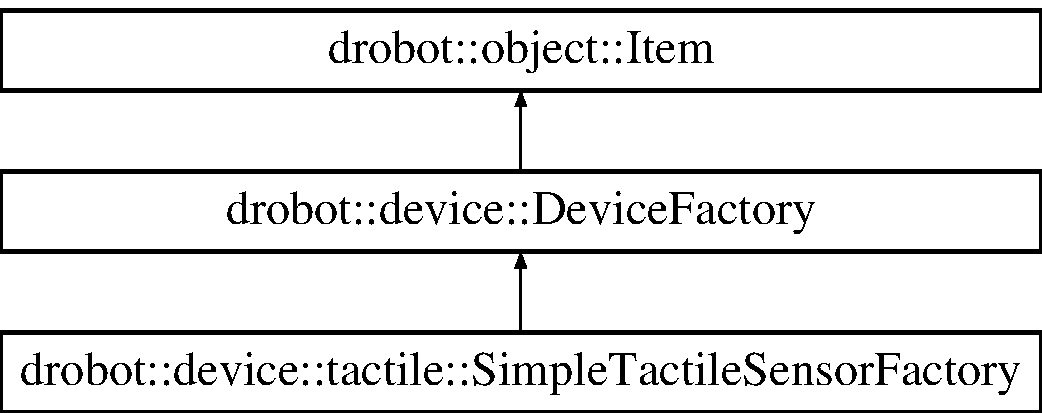
\includegraphics[height=3.000000cm]{classdrobot_1_1device_1_1tactile_1_1SimpleTactileSensorFactory}
\end{center}
\end{figure}
\subsection*{Public Member Functions}
\begin{DoxyCompactItemize}
\item 
virtual void \hyperlink{classdrobot_1_1device_1_1tactile_1_1SimpleTactileSensorFactory_a727416e619c23b25a01818e33f327d6c}{create\-From\-Dom\-Element} (Q\-Dom\-Element element, \hyperlink{classdrobot_1_1robot_1_1Robot}{robot\-::\-Robot} $\ast$robot)
\begin{DoxyCompactList}\small\item\em create\-From\-Dom\-Element \end{DoxyCompactList}\end{DoxyCompactItemize}
\subsection*{Additional Inherited Members}


\subsection{Member Function Documentation}
\hypertarget{classdrobot_1_1device_1_1tactile_1_1SimpleTactileSensorFactory_a727416e619c23b25a01818e33f327d6c}{\index{drobot\-::device\-::tactile\-::\-Simple\-Tactile\-Sensor\-Factory@{drobot\-::device\-::tactile\-::\-Simple\-Tactile\-Sensor\-Factory}!create\-From\-Dom\-Element@{create\-From\-Dom\-Element}}
\index{create\-From\-Dom\-Element@{create\-From\-Dom\-Element}!drobot::device::tactile::SimpleTactileSensorFactory@{drobot\-::device\-::tactile\-::\-Simple\-Tactile\-Sensor\-Factory}}
\subsubsection[{create\-From\-Dom\-Element}]{\setlength{\rightskip}{0pt plus 5cm}void drobot\-::device\-::tactile\-::\-Simple\-Tactile\-Sensor\-Factory\-::create\-From\-Dom\-Element (
\begin{DoxyParamCaption}
\item[{Q\-Dom\-Element}]{element, }
\item[{{\bf robot\-::\-Robot} $\ast$}]{robot}
\end{DoxyParamCaption}
)\hspace{0.3cm}{\ttfamily [virtual]}}}\label{classdrobot_1_1device_1_1tactile_1_1SimpleTactileSensorFactory_a727416e619c23b25a01818e33f327d6c}


create\-From\-Dom\-Element 


\begin{DoxyParams}{Parameters}
{\em element} & \\
\hline
{\em robot} & \\
\hline
\end{DoxyParams}
Creates a device from a Q\-Dom\-Element. This method should add the device of the robots \hyperlink{classdrobot_1_1device_1_1DeviceManager}{Device\-Manager}. If the created \hyperlink{classdrobot_1_1device_1_1Device}{Device} is a Controller the controller property of the robot should also be set. Each device element may contain channel elements which have to be parsed by the channel\-Factories. Also if the device have need of a \hyperlink{classdrobot_1_1device_1_1DeviceBoard}{Device\-Board} it should be added to the \hyperlink{classdrobot_1_1device_1_1DeviceManager}{Device\-Manager} too. See actuator/phidgetadvancedservofactory.\-cpp for an example. 

Implements \hyperlink{classdrobot_1_1device_1_1DeviceFactory_af9234abdb75d5a0129630baabe0c98cc}{drobot\-::device\-::\-Device\-Factory}.



The documentation for this class was generated from the following files\-:\begin{DoxyCompactItemize}
\item 
src/drobot/device/tactile/simpletactilesensorfactory.\-h\item 
src/drobot/device/tactile/simpletactilesensorfactory.\-cpp\end{DoxyCompactItemize}

\hypertarget{structdrobot_1_1util_1_1Source2Target}{\section{drobot\-:\-:util\-:\-:Source2\-Target$<$ Source, Target $>$ Struct Template Reference}
\label{structdrobot_1_1util_1_1Source2Target}\index{drobot\-::util\-::\-Source2\-Target$<$ Source, Target $>$@{drobot\-::util\-::\-Source2\-Target$<$ Source, Target $>$}}
}
\subsection*{Public Member Functions}
\begin{DoxyCompactItemize}
\item 
\hypertarget{structdrobot_1_1util_1_1Source2Target_aa64b7be3ffe978effc115e00bfac261d}{Target {\bfseries operator()} (Source source) const }\label{structdrobot_1_1util_1_1Source2Target_aa64b7be3ffe978effc115e00bfac261d}

\end{DoxyCompactItemize}


The documentation for this struct was generated from the following file\-:\begin{DoxyCompactItemize}
\item 
/home/imanol/workspace/drobot/new/src/drobot/util/util.\-h\end{DoxyCompactItemize}

\hypertarget{classdrobot_1_1robot_1_1event_1_1StepEvent}{\section{drobot\-:\-:robot\-:\-:event\-:\-:Step\-Event Class Reference}
\label{classdrobot_1_1robot_1_1event_1_1StepEvent}\index{drobot\-::robot\-::event\-::\-Step\-Event@{drobot\-::robot\-::event\-::\-Step\-Event}}
}


The \hyperlink{classdrobot_1_1robot_1_1event_1_1StepEvent}{Step\-Event} class. This event is fired in the robot's run method after every tick.  




{\ttfamily \#include $<$stepevent.\-h$>$}

Inheritance diagram for drobot\-:\-:robot\-:\-:event\-:\-:Step\-Event\-:\begin{figure}[H]
\begin{center}
\leavevmode
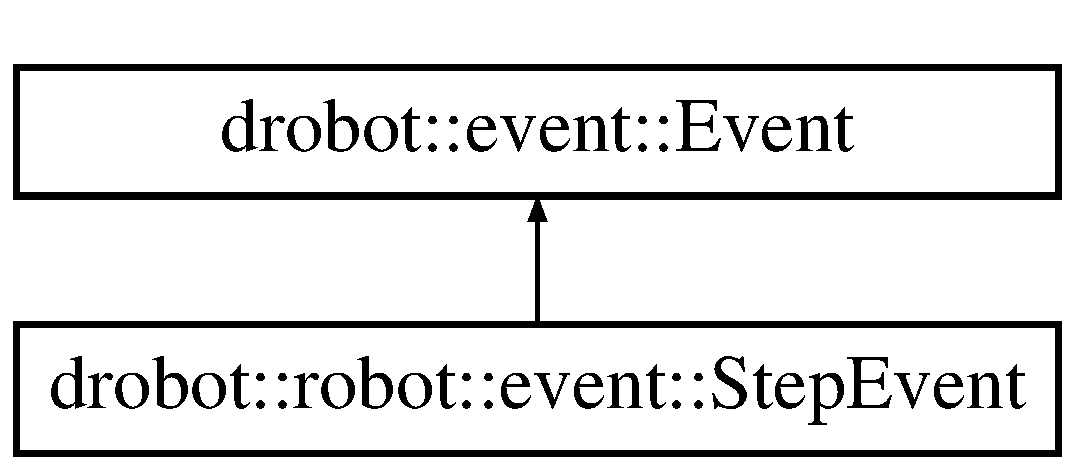
\includegraphics[height=2.000000cm]{classdrobot_1_1robot_1_1event_1_1StepEvent}
\end{center}
\end{figure}
\subsection*{Public Member Functions}
\begin{DoxyCompactItemize}
\item 
\hypertarget{classdrobot_1_1robot_1_1event_1_1StepEvent_a5e69bc4f78a26d9840e703b62d276bd2}{{\bfseries Step\-Event} (long tick, std\-::vector$<$ \hyperlink{classdrobot_1_1device_1_1channel_1_1Channel}{device\-::channel\-::\-Channel} $\ast$ $>$ channels)}\label{classdrobot_1_1robot_1_1event_1_1StepEvent_a5e69bc4f78a26d9840e703b62d276bd2}

\item 
virtual std\-::string \hyperlink{classdrobot_1_1robot_1_1event_1_1StepEvent_a40504ba9d43d9db0efdd7a16551af2f3}{to\-String} ()
\begin{DoxyCompactList}\small\item\em create a string representatio of this event used for console debugging \end{DoxyCompactList}\end{DoxyCompactItemize}
\subsection*{Private Attributes}
\begin{DoxyCompactItemize}
\item 
\hypertarget{classdrobot_1_1robot_1_1event_1_1StepEvent_aa4d308a5ee256ff10525cd09f2c3bbb7}{long {\bfseries \-\_\-tick}}\label{classdrobot_1_1robot_1_1event_1_1StepEvent_aa4d308a5ee256ff10525cd09f2c3bbb7}

\item 
\hypertarget{classdrobot_1_1robot_1_1event_1_1StepEvent_a80a1d789a30dd28a7b0981047087037b}{std\-::map\\*
$<$ \hyperlink{classdrobot_1_1device_1_1channel_1_1Channel}{device\-::channel\-::\-Channel} \\*
$\ast$, double $>$ {\bfseries \-\_\-values}}\label{classdrobot_1_1robot_1_1event_1_1StepEvent_a80a1d789a30dd28a7b0981047087037b}

\end{DoxyCompactItemize}


\subsection{Detailed Description}
The \hyperlink{classdrobot_1_1robot_1_1event_1_1StepEvent}{Step\-Event} class. This event is fired in the robot's run method after every tick. 

It contains information about the number of the tick and the current values of the different channels in the Channel\-Manager of the robot. 

\subsection{Member Function Documentation}
\hypertarget{classdrobot_1_1robot_1_1event_1_1StepEvent_a40504ba9d43d9db0efdd7a16551af2f3}{\index{drobot\-::robot\-::event\-::\-Step\-Event@{drobot\-::robot\-::event\-::\-Step\-Event}!to\-String@{to\-String}}
\index{to\-String@{to\-String}!drobot::robot::event::StepEvent@{drobot\-::robot\-::event\-::\-Step\-Event}}
\subsubsection[{to\-String}]{\setlength{\rightskip}{0pt plus 5cm}std\-::string drobot\-::robot\-::event\-::\-Step\-Event\-::to\-String (
\begin{DoxyParamCaption}
{}
\end{DoxyParamCaption}
)\hspace{0.3cm}{\ttfamily [virtual]}}}\label{classdrobot_1_1robot_1_1event_1_1StepEvent_a40504ba9d43d9db0efdd7a16551af2f3}


create a string representatio of this event used for console debugging 

\begin{DoxyReturn}{Returns}
the string representation 
\end{DoxyReturn}


Implements \hyperlink{classdrobot_1_1event_1_1Event_a25b725cbb7dbdb4a41b9c4e9fc3785d8}{drobot\-::event\-::\-Event}.



The documentation for this class was generated from the following files\-:\begin{DoxyCompactItemize}
\item 
src/drobot/robot/event/stepevent.\-h\item 
src/drobot/robot/event/stepevent.\-cpp\end{DoxyCompactItemize}

\hypertarget{classdrobot_1_1experiment_1_1tactileTest_1_1robot_1_1StupidController}{\section{drobot\-:\-:experiment\-:\-:tactile\-Test\-:\-:robot\-:\-:Stupid\-Controller Class Reference}
\label{classdrobot_1_1experiment_1_1tactileTest_1_1robot_1_1StupidController}\index{drobot\-::experiment\-::tactile\-Test\-::robot\-::\-Stupid\-Controller@{drobot\-::experiment\-::tactile\-Test\-::robot\-::\-Stupid\-Controller}}
}
Inheritance diagram for drobot\-:\-:experiment\-:\-:tactile\-Test\-:\-:robot\-:\-:Stupid\-Controller\-:\begin{figure}[H]
\begin{center}
\leavevmode
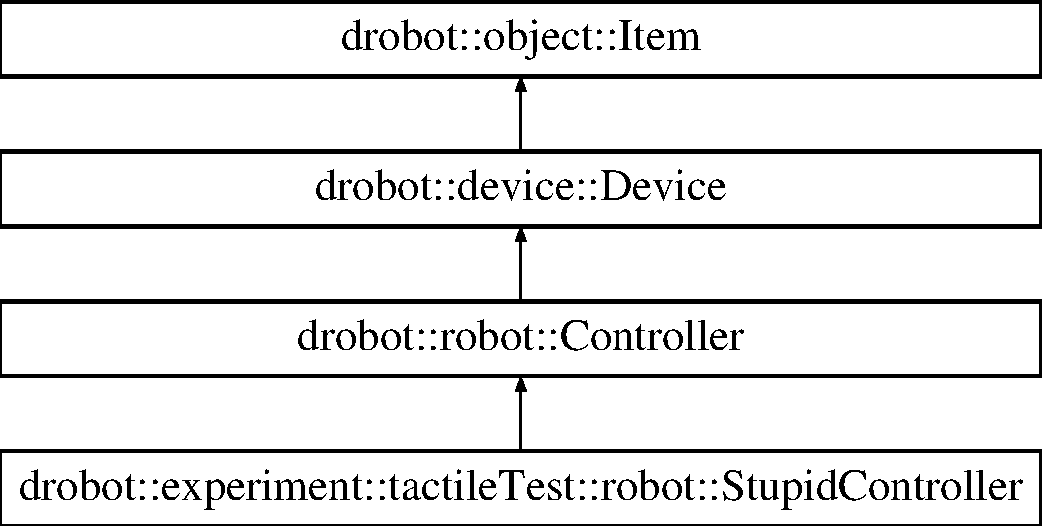
\includegraphics[height=4.000000cm]{classdrobot_1_1experiment_1_1tactileTest_1_1robot_1_1StupidController}
\end{center}
\end{figure}
\subsection*{Public Member Functions}
\begin{DoxyCompactItemize}
\item 
\hypertarget{classdrobot_1_1experiment_1_1tactileTest_1_1robot_1_1StupidController_a86aa02445fdd21422e7b66d5d233f3e5}{{\bfseries Stupid\-Controller} (std\-::string name)}\label{classdrobot_1_1experiment_1_1tactileTest_1_1robot_1_1StupidController_a86aa02445fdd21422e7b66d5d233f3e5}

\item 
virtual void \hyperlink{classdrobot_1_1experiment_1_1tactileTest_1_1robot_1_1StupidController_af18d7430f030f3cf5ce4e3d088e21ffa}{step} (long tick, \hyperlink{classdrobot_1_1device_1_1channel_1_1ChannelManager}{device\-::channel\-::\-Channel\-Manager} $\ast$channels)
\begin{DoxyCompactList}\small\item\em This function is called at a specific frequency defined in the Robot. \end{DoxyCompactList}\end{DoxyCompactItemize}
\subsection*{Additional Inherited Members}


\subsection{Member Function Documentation}
\hypertarget{classdrobot_1_1experiment_1_1tactileTest_1_1robot_1_1StupidController_af18d7430f030f3cf5ce4e3d088e21ffa}{\index{drobot\-::experiment\-::tactile\-Test\-::robot\-::\-Stupid\-Controller@{drobot\-::experiment\-::tactile\-Test\-::robot\-::\-Stupid\-Controller}!step@{step}}
\index{step@{step}!drobot::experiment::tactileTest::robot::StupidController@{drobot\-::experiment\-::tactile\-Test\-::robot\-::\-Stupid\-Controller}}
\subsubsection[{step}]{\setlength{\rightskip}{0pt plus 5cm}void drobot\-::experiment\-::tactile\-Test\-::robot\-::\-Stupid\-Controller\-::step (
\begin{DoxyParamCaption}
\item[{long}]{tick, }
\item[{{\bf device\-::channel\-::\-Channel\-Manager} $\ast$}]{channels}
\end{DoxyParamCaption}
)\hspace{0.3cm}{\ttfamily [virtual]}}}\label{classdrobot_1_1experiment_1_1tactileTest_1_1robot_1_1StupidController_af18d7430f030f3cf5ce4e3d088e21ffa}


This function is called at a specific frequency defined in the Robot. 

This method should first read the values of the input channels, then calculate the output and write it to the output channels. Additionally other stuff can be written to log channels for logging. 
\begin{DoxyParams}{Parameters}
{\em tick} & the timestep \\
\hline
{\em channels} & of the robot \\
\hline
\end{DoxyParams}


Implements \hyperlink{classdrobot_1_1robot_1_1Controller_acbbde3e529dad162fb36074c7e25a924}{drobot\-::robot\-::\-Controller}.



The documentation for this class was generated from the following files\-:\begin{DoxyCompactItemize}
\item 
src/drobot/experiment/tactile\-Test/robot/stupidcontroller.\-h\item 
src/drobot/experiment/tactile\-Test/robot/stupidcontroller.\-cpp\end{DoxyCompactItemize}

\hypertarget{classdrobot_1_1experiment_1_1tactileTest_1_1robot_1_1StupidControllerFactory}{\section{drobot\-:\-:experiment\-:\-:tactile\-Test\-:\-:robot\-:\-:Stupid\-Controller\-Factory Class Reference}
\label{classdrobot_1_1experiment_1_1tactileTest_1_1robot_1_1StupidControllerFactory}\index{drobot\-::experiment\-::tactile\-Test\-::robot\-::\-Stupid\-Controller\-Factory@{drobot\-::experiment\-::tactile\-Test\-::robot\-::\-Stupid\-Controller\-Factory}}
}
Inheritance diagram for drobot\-:\-:experiment\-:\-:tactile\-Test\-:\-:robot\-:\-:Stupid\-Controller\-Factory\-:\begin{figure}[H]
\begin{center}
\leavevmode
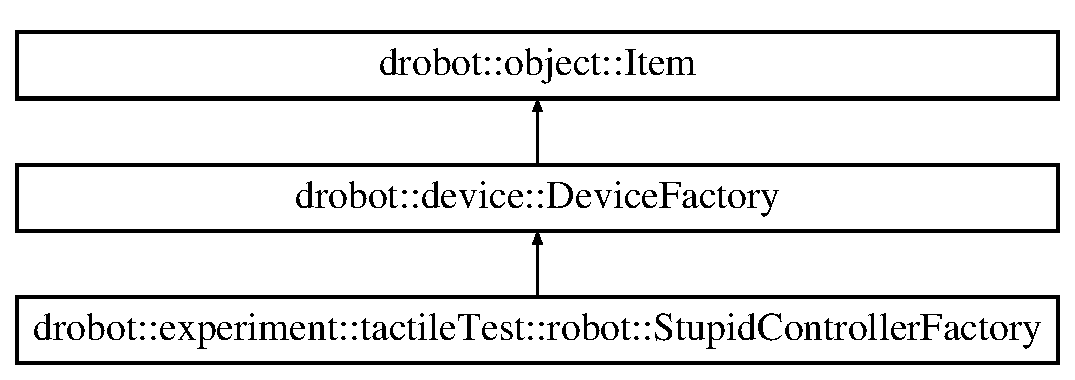
\includegraphics[height=3.000000cm]{classdrobot_1_1experiment_1_1tactileTest_1_1robot_1_1StupidControllerFactory}
\end{center}
\end{figure}
\subsection*{Public Member Functions}
\begin{DoxyCompactItemize}
\item 
virtual void \hyperlink{classdrobot_1_1experiment_1_1tactileTest_1_1robot_1_1StupidControllerFactory_aa5d84ac226f532590642a76a74e8df96}{create\-From\-Dom\-Element} (Q\-Dom\-Element element, \hyperlink{classdrobot_1_1robot_1_1Robot}{drobot\-::robot\-::\-Robot} $\ast$robot)
\begin{DoxyCompactList}\small\item\em create\-From\-Dom\-Element \end{DoxyCompactList}\end{DoxyCompactItemize}
\subsection*{Additional Inherited Members}


\subsection{Member Function Documentation}
\hypertarget{classdrobot_1_1experiment_1_1tactileTest_1_1robot_1_1StupidControllerFactory_aa5d84ac226f532590642a76a74e8df96}{\index{drobot\-::experiment\-::tactile\-Test\-::robot\-::\-Stupid\-Controller\-Factory@{drobot\-::experiment\-::tactile\-Test\-::robot\-::\-Stupid\-Controller\-Factory}!create\-From\-Dom\-Element@{create\-From\-Dom\-Element}}
\index{create\-From\-Dom\-Element@{create\-From\-Dom\-Element}!drobot::experiment::tactileTest::robot::StupidControllerFactory@{drobot\-::experiment\-::tactile\-Test\-::robot\-::\-Stupid\-Controller\-Factory}}
\subsubsection[{create\-From\-Dom\-Element}]{\setlength{\rightskip}{0pt plus 5cm}void drobot\-::experiment\-::tactile\-Test\-::robot\-::\-Stupid\-Controller\-Factory\-::create\-From\-Dom\-Element (
\begin{DoxyParamCaption}
\item[{Q\-Dom\-Element}]{element, }
\item[{{\bf drobot\-::robot\-::\-Robot} $\ast$}]{robot}
\end{DoxyParamCaption}
)\hspace{0.3cm}{\ttfamily [virtual]}}}\label{classdrobot_1_1experiment_1_1tactileTest_1_1robot_1_1StupidControllerFactory_aa5d84ac226f532590642a76a74e8df96}


create\-From\-Dom\-Element 


\begin{DoxyParams}{Parameters}
{\em element} & \\
\hline
{\em robot} & \\
\hline
\end{DoxyParams}
Creates a device from a Q\-Dom\-Element. This method should add the device of the robots Device\-Manager. If the created Device is a Controller the controller property of the robot should also be set. Each device element may contain channel elements which have to be parsed by the channel\-Factories. Also if the device have need of a Device\-Board it should be added to the Device\-Manager too. See actuator/phidgetadvancedservofactory.\-cpp for an example. 

Implements \hyperlink{classdrobot_1_1device_1_1DeviceFactory_af9234abdb75d5a0129630baabe0c98cc}{drobot\-::device\-::\-Device\-Factory}.



The documentation for this class was generated from the following files\-:\begin{DoxyCompactItemize}
\item 
src/drobot/experiment/tactile\-Test/robot/stupidcontrollerfactory.\-h\item 
src/drobot/experiment/tactile\-Test/robot/stupidcontrollerfactory.\-cpp\end{DoxyCompactItemize}

\hypertarget{classdrobot_1_1device_1_1tactile_1_1TactileSensor}{\section{drobot\-:\-:device\-:\-:tactile\-:\-:Tactile\-Sensor Class Reference}
\label{classdrobot_1_1device_1_1tactile_1_1TactileSensor}\index{drobot\-::device\-::tactile\-::\-Tactile\-Sensor@{drobot\-::device\-::tactile\-::\-Tactile\-Sensor}}
}


Base class for all tactile sensors.  




{\ttfamily \#include $<$tactilesensor.\-h$>$}

Inheritance diagram for drobot\-:\-:device\-:\-:tactile\-:\-:Tactile\-Sensor\-:\begin{figure}[H]
\begin{center}
\leavevmode
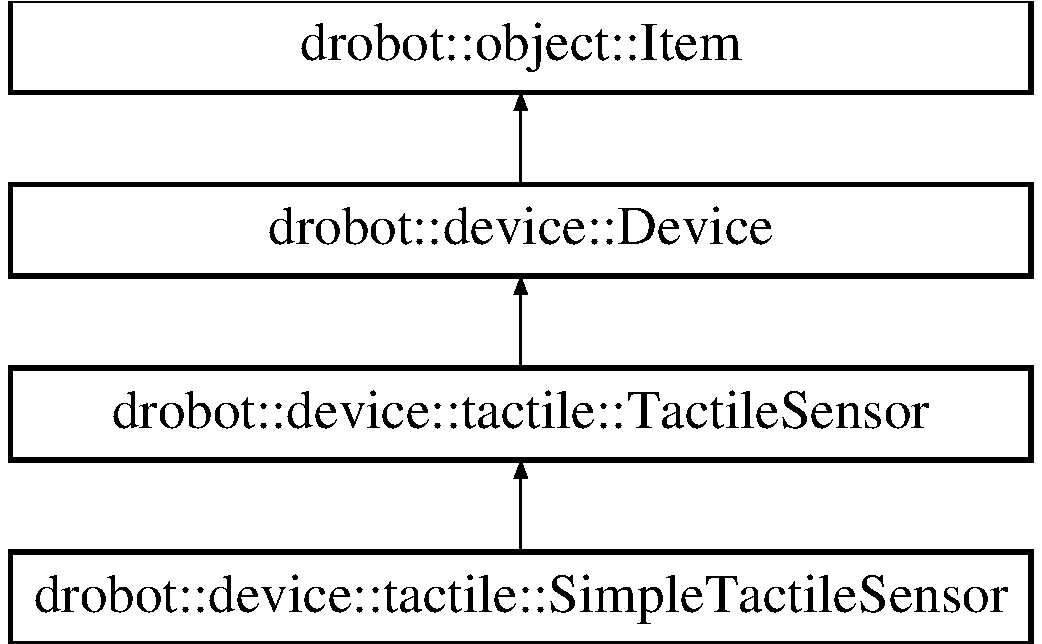
\includegraphics[height=4.000000cm]{classdrobot_1_1device_1_1tactile_1_1TactileSensor}
\end{center}
\end{figure}
\subsection*{Public Member Functions}
\begin{DoxyCompactItemize}
\item 
\hypertarget{classdrobot_1_1device_1_1tactile_1_1TactileSensor_ade88271b8e2ca587e8b45935c30bdacb}{{\bfseries Tactile\-Sensor} (std\-::string name)}\label{classdrobot_1_1device_1_1tactile_1_1TactileSensor_ade88271b8e2ca587e8b45935c30bdacb}

\item 
virtual double \hyperlink{classdrobot_1_1device_1_1tactile_1_1TactileSensor_a89fd3eb13e03638fba38fa6a4b8d17ed}{get\-Value} ()=0
\item 
virtual double \hyperlink{classdrobot_1_1device_1_1tactile_1_1TactileSensor_ae586a70280096eb764188a94c9044470}{get\-Value\-Min} ()=0
\item 
virtual double \hyperlink{classdrobot_1_1device_1_1tactile_1_1TactileSensor_a03eb99ccdc4bb78818ce556c440d372a}{get\-Value\-Max} ()=0
\end{DoxyCompactItemize}
\subsection*{Additional Inherited Members}


\subsection{Detailed Description}
Base class for all tactile sensors. 

\subsection{Member Function Documentation}
\hypertarget{classdrobot_1_1device_1_1tactile_1_1TactileSensor_a89fd3eb13e03638fba38fa6a4b8d17ed}{\index{drobot\-::device\-::tactile\-::\-Tactile\-Sensor@{drobot\-::device\-::tactile\-::\-Tactile\-Sensor}!get\-Value@{get\-Value}}
\index{get\-Value@{get\-Value}!drobot::device::tactile::TactileSensor@{drobot\-::device\-::tactile\-::\-Tactile\-Sensor}}
\subsubsection[{get\-Value}]{\setlength{\rightskip}{0pt plus 5cm}virtual double drobot\-::device\-::tactile\-::\-Tactile\-Sensor\-::get\-Value (
\begin{DoxyParamCaption}
{}
\end{DoxyParamCaption}
)\hspace{0.3cm}{\ttfamily [pure virtual]}}}\label{classdrobot_1_1device_1_1tactile_1_1TactileSensor_a89fd3eb13e03638fba38fa6a4b8d17ed}
\begin{DoxyReturn}{Returns}
current value of the tactile sensor 
\end{DoxyReturn}


Implemented in \hyperlink{classdrobot_1_1device_1_1tactile_1_1SimpleTactileSensor_a8f9d1aec99cd3c53bac343af3a3bda60}{drobot\-::device\-::tactile\-::\-Simple\-Tactile\-Sensor}.

\hypertarget{classdrobot_1_1device_1_1tactile_1_1TactileSensor_a03eb99ccdc4bb78818ce556c440d372a}{\index{drobot\-::device\-::tactile\-::\-Tactile\-Sensor@{drobot\-::device\-::tactile\-::\-Tactile\-Sensor}!get\-Value\-Max@{get\-Value\-Max}}
\index{get\-Value\-Max@{get\-Value\-Max}!drobot::device::tactile::TactileSensor@{drobot\-::device\-::tactile\-::\-Tactile\-Sensor}}
\subsubsection[{get\-Value\-Max}]{\setlength{\rightskip}{0pt plus 5cm}virtual double drobot\-::device\-::tactile\-::\-Tactile\-Sensor\-::get\-Value\-Max (
\begin{DoxyParamCaption}
{}
\end{DoxyParamCaption}
)\hspace{0.3cm}{\ttfamily [pure virtual]}}}\label{classdrobot_1_1device_1_1tactile_1_1TactileSensor_a03eb99ccdc4bb78818ce556c440d372a}
\begin{DoxyReturn}{Returns}
maximal possible value 
\end{DoxyReturn}


Implemented in \hyperlink{classdrobot_1_1device_1_1tactile_1_1SimpleTactileSensor_aa5e6c1634c8fafe61e41cb998c02b6b6}{drobot\-::device\-::tactile\-::\-Simple\-Tactile\-Sensor}.

\hypertarget{classdrobot_1_1device_1_1tactile_1_1TactileSensor_ae586a70280096eb764188a94c9044470}{\index{drobot\-::device\-::tactile\-::\-Tactile\-Sensor@{drobot\-::device\-::tactile\-::\-Tactile\-Sensor}!get\-Value\-Min@{get\-Value\-Min}}
\index{get\-Value\-Min@{get\-Value\-Min}!drobot::device::tactile::TactileSensor@{drobot\-::device\-::tactile\-::\-Tactile\-Sensor}}
\subsubsection[{get\-Value\-Min}]{\setlength{\rightskip}{0pt plus 5cm}virtual double drobot\-::device\-::tactile\-::\-Tactile\-Sensor\-::get\-Value\-Min (
\begin{DoxyParamCaption}
{}
\end{DoxyParamCaption}
)\hspace{0.3cm}{\ttfamily [pure virtual]}}}\label{classdrobot_1_1device_1_1tactile_1_1TactileSensor_ae586a70280096eb764188a94c9044470}
\begin{DoxyReturn}{Returns}
minimal possible value 
\end{DoxyReturn}


Implemented in \hyperlink{classdrobot_1_1device_1_1tactile_1_1SimpleTactileSensor_aff61edb7f9ccdac4f0209590bb8d7d76}{drobot\-::device\-::tactile\-::\-Simple\-Tactile\-Sensor}.



The documentation for this class was generated from the following files\-:\begin{DoxyCompactItemize}
\item 
/home/imanol/workspace/drobot/new/src/drobot/device/tactile/tactilesensor.\-h\item 
/home/imanol/workspace/drobot/new/src/drobot/device/tactile/tactilesensor.\-cpp\end{DoxyCompactItemize}

\hypertarget{classdrobot_1_1device_1_1tactile_1_1TactileSensorBoard}{\section{drobot\-:\-:device\-:\-:tactile\-:\-:Tactile\-Sensor\-Board Class Reference}
\label{classdrobot_1_1device_1_1tactile_1_1TactileSensorBoard}\index{drobot\-::device\-::tactile\-::\-Tactile\-Sensor\-Board@{drobot\-::device\-::tactile\-::\-Tactile\-Sensor\-Board}}
}
Inheritance diagram for drobot\-:\-:device\-:\-:tactile\-:\-:Tactile\-Sensor\-Board\-:\begin{figure}[H]
\begin{center}
\leavevmode
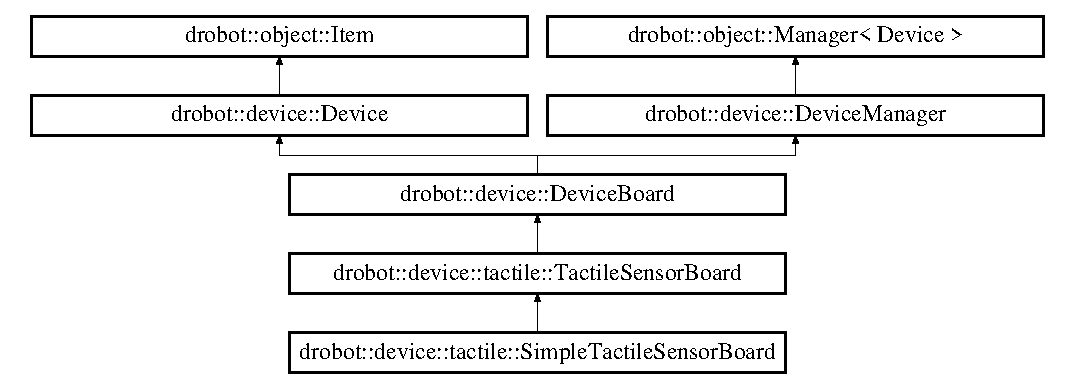
\includegraphics[height=4.778157cm]{classdrobot_1_1device_1_1tactile_1_1TactileSensorBoard}
\end{center}
\end{figure}
\subsection*{Public Member Functions}
\begin{DoxyCompactItemize}
\item 
\hypertarget{classdrobot_1_1device_1_1tactile_1_1TactileSensorBoard_afe6aa518491c12cfe7f11011473bea0c}{{\bfseries Tactile\-Sensor\-Board} (std\-::string name)}\label{classdrobot_1_1device_1_1tactile_1_1TactileSensorBoard_afe6aa518491c12cfe7f11011473bea0c}

\item 
\hypertarget{classdrobot_1_1device_1_1tactile_1_1TactileSensorBoard_a5663bddd91d2fc3c54f00a5a7a10d91f}{std\-::vector$<$ \hyperlink{classdrobot_1_1device_1_1tactile_1_1TactileSensor}{Tactile\-Sensor} $\ast$ $>$ {\bfseries get\-Tactile\-Sensors} ()}\label{classdrobot_1_1device_1_1tactile_1_1TactileSensorBoard_a5663bddd91d2fc3c54f00a5a7a10d91f}

\item 
\hypertarget{classdrobot_1_1device_1_1tactile_1_1TactileSensorBoard_a1fe8a3ffa05557b3069a789090f2bc61}{\hyperlink{classdrobot_1_1device_1_1tactile_1_1TactileSensor}{Tactile\-Sensor} $\ast$ {\bfseries get\-Tactile\-Sensor} (std\-::string name)}\label{classdrobot_1_1device_1_1tactile_1_1TactileSensorBoard_a1fe8a3ffa05557b3069a789090f2bc61}

\end{DoxyCompactItemize}
\subsection*{Additional Inherited Members}


The documentation for this class was generated from the following files\-:\begin{DoxyCompactItemize}
\item 
/home/imanol/workspace/drobot/new/src/drobot/device/tactile/tactilesensorboard.\-h\item 
/home/imanol/workspace/drobot/new/src/drobot/device/tactile/tactilesensorboard.\-cpp\end{DoxyCompactItemize}

\hypertarget{classdrobot_1_1device_1_1tactile_1_1channel_1_1TactileSensorValueChannel}{\section{drobot\-:\-:device\-:\-:tactile\-:\-:channel\-:\-:Tactile\-Sensor\-Value\-Channel Class Reference}
\label{classdrobot_1_1device_1_1tactile_1_1channel_1_1TactileSensorValueChannel}\index{drobot\-::device\-::tactile\-::channel\-::\-Tactile\-Sensor\-Value\-Channel@{drobot\-::device\-::tactile\-::channel\-::\-Tactile\-Sensor\-Value\-Channel}}
}
Inheritance diagram for drobot\-:\-:device\-:\-:tactile\-:\-:channel\-:\-:Tactile\-Sensor\-Value\-Channel\-:\begin{figure}[H]
\begin{center}
\leavevmode
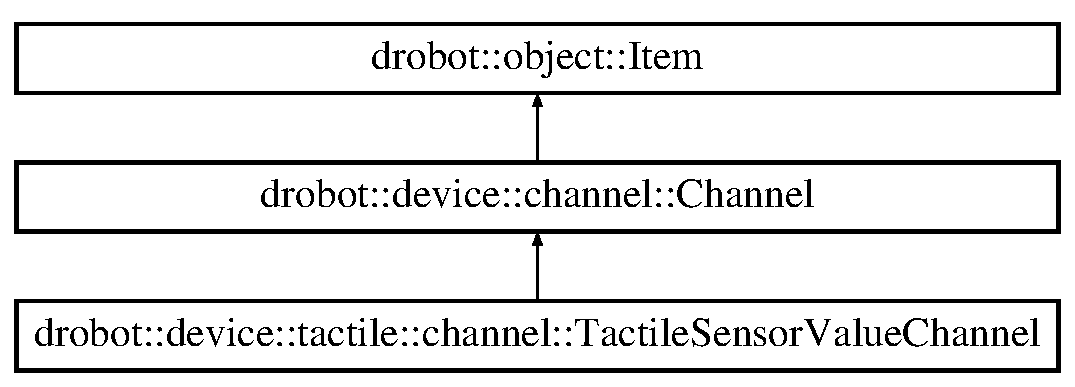
\includegraphics[height=3.000000cm]{classdrobot_1_1device_1_1tactile_1_1channel_1_1TactileSensorValueChannel}
\end{center}
\end{figure}
\subsection*{Public Member Functions}
\begin{DoxyCompactItemize}
\item 
\hypertarget{classdrobot_1_1device_1_1tactile_1_1channel_1_1TactileSensorValueChannel_a8ea17745d81716bed41136ef4cb62d5f}{{\bfseries Tactile\-Sensor\-Value\-Channel} (std\-::string name, device\-::channel\-::\-Channel\-Type type)}\label{classdrobot_1_1device_1_1tactile_1_1channel_1_1TactileSensorValueChannel_a8ea17745d81716bed41136ef4cb62d5f}

\item 
\hypertarget{classdrobot_1_1device_1_1tactile_1_1channel_1_1TactileSensorValueChannel_ac3175e796c2e1b3d5bf1efabe2650927}{{\bfseries Tactile\-Sensor\-Value\-Channel} (std\-::string name, device\-::channel\-::\-Channel\-Type type, \hyperlink{classdrobot_1_1device_1_1channel_1_1Normalizer}{device\-::channel\-::\-Normalizer} $\ast$normalizer, \hyperlink{classdrobot_1_1device_1_1Device}{device\-::\-Device} $\ast$device)}\label{classdrobot_1_1device_1_1tactile_1_1channel_1_1TactileSensorValueChannel_ac3175e796c2e1b3d5bf1efabe2650927}

\end{DoxyCompactItemize}
\subsection*{Protected Member Functions}
\begin{DoxyCompactItemize}
\item 
virtual void \hyperlink{classdrobot_1_1device_1_1tactile_1_1channel_1_1TactileSensorValueChannel_af98159e60d1bc3ebfff9135c179f4287}{set\-Value} (double value)
\begin{DoxyCompactList}\small\item\em sets the value directly to the device \end{DoxyCompactList}\item 
virtual double \hyperlink{classdrobot_1_1device_1_1tactile_1_1channel_1_1TactileSensorValueChannel_a84465511da1c70beb14508828243ff6d}{get\-Value} ()
\begin{DoxyCompactList}\small\item\em returns the value directly from the device. \end{DoxyCompactList}\end{DoxyCompactItemize}
\subsection*{Additional Inherited Members}


\subsection{Member Function Documentation}
\hypertarget{classdrobot_1_1device_1_1tactile_1_1channel_1_1TactileSensorValueChannel_a84465511da1c70beb14508828243ff6d}{\index{drobot\-::device\-::tactile\-::channel\-::\-Tactile\-Sensor\-Value\-Channel@{drobot\-::device\-::tactile\-::channel\-::\-Tactile\-Sensor\-Value\-Channel}!get\-Value@{get\-Value}}
\index{get\-Value@{get\-Value}!drobot::device::tactile::channel::TactileSensorValueChannel@{drobot\-::device\-::tactile\-::channel\-::\-Tactile\-Sensor\-Value\-Channel}}
\subsubsection[{get\-Value}]{\setlength{\rightskip}{0pt plus 5cm}double drobot\-::device\-::tactile\-::channel\-::\-Tactile\-Sensor\-Value\-Channel\-::get\-Value (
\begin{DoxyParamCaption}
{}
\end{DoxyParamCaption}
)\hspace{0.3cm}{\ttfamily [protected]}, {\ttfamily [virtual]}}}\label{classdrobot_1_1device_1_1tactile_1_1channel_1_1TactileSensorValueChannel_a84465511da1c70beb14508828243ff6d}


returns the value directly from the device. 

\begin{DoxyReturn}{Returns}

\end{DoxyReturn}


Implements \hyperlink{classdrobot_1_1device_1_1channel_1_1Channel_a42f0978ebb99d13a89c1785baf69a4d8}{drobot\-::device\-::channel\-::\-Channel}.

\hypertarget{classdrobot_1_1device_1_1tactile_1_1channel_1_1TactileSensorValueChannel_af98159e60d1bc3ebfff9135c179f4287}{\index{drobot\-::device\-::tactile\-::channel\-::\-Tactile\-Sensor\-Value\-Channel@{drobot\-::device\-::tactile\-::channel\-::\-Tactile\-Sensor\-Value\-Channel}!set\-Value@{set\-Value}}
\index{set\-Value@{set\-Value}!drobot::device::tactile::channel::TactileSensorValueChannel@{drobot\-::device\-::tactile\-::channel\-::\-Tactile\-Sensor\-Value\-Channel}}
\subsubsection[{set\-Value}]{\setlength{\rightskip}{0pt plus 5cm}void drobot\-::device\-::tactile\-::channel\-::\-Tactile\-Sensor\-Value\-Channel\-::set\-Value (
\begin{DoxyParamCaption}
\item[{double}]{value}
\end{DoxyParamCaption}
)\hspace{0.3cm}{\ttfamily [protected]}, {\ttfamily [virtual]}}}\label{classdrobot_1_1device_1_1tactile_1_1channel_1_1TactileSensorValueChannel_af98159e60d1bc3ebfff9135c179f4287}


sets the value directly to the device 


\begin{DoxyParams}{Parameters}
{\em value} & \\
\hline
\end{DoxyParams}


Implements \hyperlink{classdrobot_1_1device_1_1channel_1_1Channel_a612a3f6afe59e238583d6d40d9ddcaf8}{drobot\-::device\-::channel\-::\-Channel}.



The documentation for this class was generated from the following files\-:\begin{DoxyCompactItemize}
\item 
src/drobot/device/tactile/channel/tactilesensorvaluechannel.\-h\item 
src/drobot/device/tactile/channel/tactilesensorvaluechannel.\-cpp\end{DoxyCompactItemize}

\hypertarget{classdrobot_1_1device_1_1tactile_1_1channel_1_1TactileSensorValueChannelFactory}{\section{drobot\-:\-:device\-:\-:tactile\-:\-:channel\-:\-:Tactile\-Sensor\-Value\-Channel\-Factory Class Reference}
\label{classdrobot_1_1device_1_1tactile_1_1channel_1_1TactileSensorValueChannelFactory}\index{drobot\-::device\-::tactile\-::channel\-::\-Tactile\-Sensor\-Value\-Channel\-Factory@{drobot\-::device\-::tactile\-::channel\-::\-Tactile\-Sensor\-Value\-Channel\-Factory}}
}
Inheritance diagram for drobot\-:\-:device\-:\-:tactile\-:\-:channel\-:\-:Tactile\-Sensor\-Value\-Channel\-Factory\-:\begin{figure}[H]
\begin{center}
\leavevmode
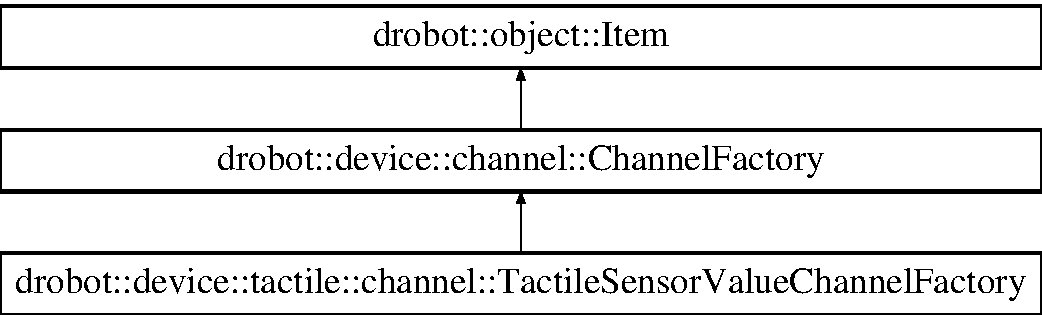
\includegraphics[height=3.000000cm]{classdrobot_1_1device_1_1tactile_1_1channel_1_1TactileSensorValueChannelFactory}
\end{center}
\end{figure}
\subsection*{Public Member Functions}
\begin{DoxyCompactItemize}
\item 
virtual void \hyperlink{classdrobot_1_1device_1_1tactile_1_1channel_1_1TactileSensorValueChannelFactory_a2e4369c57cdd99f2c59469f6451e4c0c}{create\-From\-Dom\-Element} (Q\-Dom\-Element element, \hyperlink{classdrobot_1_1device_1_1Device}{Device} $\ast$device)
\begin{DoxyCompactList}\small\item\em create channel from Dom Tree element \end{DoxyCompactList}\end{DoxyCompactItemize}
\subsection*{Additional Inherited Members}


\subsection{Member Function Documentation}
\hypertarget{classdrobot_1_1device_1_1tactile_1_1channel_1_1TactileSensorValueChannelFactory_a2e4369c57cdd99f2c59469f6451e4c0c}{\index{drobot\-::device\-::tactile\-::channel\-::\-Tactile\-Sensor\-Value\-Channel\-Factory@{drobot\-::device\-::tactile\-::channel\-::\-Tactile\-Sensor\-Value\-Channel\-Factory}!create\-From\-Dom\-Element@{create\-From\-Dom\-Element}}
\index{create\-From\-Dom\-Element@{create\-From\-Dom\-Element}!drobot::device::tactile::channel::TactileSensorValueChannelFactory@{drobot\-::device\-::tactile\-::channel\-::\-Tactile\-Sensor\-Value\-Channel\-Factory}}
\subsubsection[{create\-From\-Dom\-Element}]{\setlength{\rightskip}{0pt plus 5cm}void drobot\-::device\-::tactile\-::channel\-::\-Tactile\-Sensor\-Value\-Channel\-Factory\-::create\-From\-Dom\-Element (
\begin{DoxyParamCaption}
\item[{Q\-Dom\-Element}]{element, }
\item[{{\bf Device} $\ast$}]{device}
\end{DoxyParamCaption}
)\hspace{0.3cm}{\ttfamily [virtual]}}}\label{classdrobot_1_1device_1_1tactile_1_1channel_1_1TactileSensorValueChannelFactory_a2e4369c57cdd99f2c59469f6451e4c0c}


create channel from Dom Tree element 

this method has to create one or more channels from the element and add it to the device. 
\begin{DoxyParams}{Parameters}
{\em element} & \\
\hline
{\em device} & \\
\hline
\end{DoxyParams}


Implements \hyperlink{classdrobot_1_1device_1_1channel_1_1ChannelFactory_ab59ee44782347b8878a471bf87f06c43}{drobot\-::device\-::channel\-::\-Channel\-Factory}.



The documentation for this class was generated from the following files\-:\begin{DoxyCompactItemize}
\item 
/home/imanol/workspace/drobot/new/src/drobot/device/tactile/channel/tactilesensorvaluechannelfactory.\-h\item 
/home/imanol/workspace/drobot/new/src/drobot/device/tactile/channel/tactilesensorvaluechannelfactory.\-cpp\end{DoxyCompactItemize}

\hypertarget{classdrobot_1_1device_1_1vestibular_1_1Vestibular}{\section{drobot\-:\-:device\-:\-:vestibular\-:\-:Vestibular Class Reference}
\label{classdrobot_1_1device_1_1vestibular_1_1Vestibular}\index{drobot\-::device\-::vestibular\-::\-Vestibular@{drobot\-::device\-::vestibular\-::\-Vestibular}}
}


The \hyperlink{classdrobot_1_1device_1_1vestibular_1_1Vestibular}{Vestibular} class is the base for all \hyperlink{classdrobot_1_1device_1_1vestibular_1_1Vestibular}{Vestibular} system like sensors.  




{\ttfamily \#include $<$vestibular.\-h$>$}

Inheritance diagram for drobot\-:\-:device\-:\-:vestibular\-:\-:Vestibular\-:\begin{figure}[H]
\begin{center}
\leavevmode
\includegraphics[height=4.000000cm]{classdrobot_1_1device_1_1vestibular_1_1Vestibular}
\end{center}
\end{figure}
\subsection*{Public Member Functions}
\begin{DoxyCompactItemize}
\item 
\hypertarget{classdrobot_1_1device_1_1vestibular_1_1Vestibular_a29c17eac2af0c2e974d3531b8d53a3aa}{{\bfseries Vestibular} (std\-::string name)}\label{classdrobot_1_1device_1_1vestibular_1_1Vestibular_a29c17eac2af0c2e974d3531b8d53a3aa}

\item 
virtual std\-::vector$<$ double $>$ \hyperlink{classdrobot_1_1device_1_1vestibular_1_1Vestibular_a603a1a556bc01d05fbcdc152fcac187e}{get\-Acceleration} ()=0
\begin{DoxyCompactList}\small\item\em get\-Acceleration \end{DoxyCompactList}\item 
virtual std\-::vector$<$ double $>$ \hyperlink{classdrobot_1_1device_1_1vestibular_1_1Vestibular_aa8b4a963dabe11f217e6ec3f589b67c9}{get\-Acceleration\-Min} ()=0
\begin{DoxyCompactList}\small\item\em get\-Acceleration\-Min \end{DoxyCompactList}\item 
virtual std\-::vector$<$ double $>$ \hyperlink{classdrobot_1_1device_1_1vestibular_1_1Vestibular_a373ed8304b4dce771493da5a1a88de81}{get\-Acceleration\-Max} ()=0
\begin{DoxyCompactList}\small\item\em get\-Acceleration\-Max \end{DoxyCompactList}\item 
virtual std\-::vector$<$ double $>$ \hyperlink{classdrobot_1_1device_1_1vestibular_1_1Vestibular_adcd46ff2d7971a57550b4221c268eb93}{get\-Angular\-Rate} ()=0
\begin{DoxyCompactList}\small\item\em get\-Angular\-Rate \end{DoxyCompactList}\item 
virtual std\-::vector$<$ double $>$ \hyperlink{classdrobot_1_1device_1_1vestibular_1_1Vestibular_ad49879a49bf891eaf8aa31127a05f69c}{get\-Angular\-Rate\-Min} ()=0
\begin{DoxyCompactList}\small\item\em get\-Angular\-Rate\-Min \end{DoxyCompactList}\item 
virtual std\-::vector$<$ double $>$ \hyperlink{classdrobot_1_1device_1_1vestibular_1_1Vestibular_aa8b14d53824fab9b37d1009a43d2000f}{get\-Angular\-Rate\-Max} ()=0
\begin{DoxyCompactList}\small\item\em get\-Angular\-Rate\-Max \end{DoxyCompactList}\item 
virtual std\-::vector$<$ double $>$ \hyperlink{classdrobot_1_1device_1_1vestibular_1_1Vestibular_af916767f525fde239401392308ebdd2d}{get\-Magnetic\-Field} ()=0
\begin{DoxyCompactList}\small\item\em get\-Magnetic\-Field \end{DoxyCompactList}\item 
virtual std\-::vector$<$ double $>$ \hyperlink{classdrobot_1_1device_1_1vestibular_1_1Vestibular_aedf3e81c5256febccfc8514fa3368322}{get\-Magnetic\-Field\-Min} ()=0
\begin{DoxyCompactList}\small\item\em get\-Magnetic\-Field\-Min \end{DoxyCompactList}\item 
virtual std\-::vector$<$ double $>$ \hyperlink{classdrobot_1_1device_1_1vestibular_1_1Vestibular_a47dcc13aab2c15633d25f33c92de035e}{get\-Magnetic\-Field\-Max} ()=0
\begin{DoxyCompactList}\small\item\em get\-Magnetic\-Field\-Max \end{DoxyCompactList}\end{DoxyCompactItemize}
\subsection*{Additional Inherited Members}


\subsection{Detailed Description}
The \hyperlink{classdrobot_1_1device_1_1vestibular_1_1Vestibular}{Vestibular} class is the base for all \hyperlink{classdrobot_1_1device_1_1vestibular_1_1Vestibular}{Vestibular} system like sensors. 

\subsection{Member Function Documentation}
\hypertarget{classdrobot_1_1device_1_1vestibular_1_1Vestibular_a603a1a556bc01d05fbcdc152fcac187e}{\index{drobot\-::device\-::vestibular\-::\-Vestibular@{drobot\-::device\-::vestibular\-::\-Vestibular}!get\-Acceleration@{get\-Acceleration}}
\index{get\-Acceleration@{get\-Acceleration}!drobot::device::vestibular::Vestibular@{drobot\-::device\-::vestibular\-::\-Vestibular}}
\subsubsection[{get\-Acceleration}]{\setlength{\rightskip}{0pt plus 5cm}virtual std\-::vector$<$double$>$ drobot\-::device\-::vestibular\-::\-Vestibular\-::get\-Acceleration (
\begin{DoxyParamCaption}
{}
\end{DoxyParamCaption}
)\hspace{0.3cm}{\ttfamily [pure virtual]}}}\label{classdrobot_1_1device_1_1vestibular_1_1Vestibular_a603a1a556bc01d05fbcdc152fcac187e}


get\-Acceleration 

\begin{DoxyReturn}{Returns}
acceleration vector 
\end{DoxyReturn}


Implemented in \hyperlink{classdrobot_1_1device_1_1vestibular_1_1PhidgetVestibular_a70f361e5840a67882a5dfbe486e8c0ad}{drobot\-::device\-::vestibular\-::\-Phidget\-Vestibular}.

\hypertarget{classdrobot_1_1device_1_1vestibular_1_1Vestibular_a373ed8304b4dce771493da5a1a88de81}{\index{drobot\-::device\-::vestibular\-::\-Vestibular@{drobot\-::device\-::vestibular\-::\-Vestibular}!get\-Acceleration\-Max@{get\-Acceleration\-Max}}
\index{get\-Acceleration\-Max@{get\-Acceleration\-Max}!drobot::device::vestibular::Vestibular@{drobot\-::device\-::vestibular\-::\-Vestibular}}
\subsubsection[{get\-Acceleration\-Max}]{\setlength{\rightskip}{0pt plus 5cm}virtual std\-::vector$<$double$>$ drobot\-::device\-::vestibular\-::\-Vestibular\-::get\-Acceleration\-Max (
\begin{DoxyParamCaption}
{}
\end{DoxyParamCaption}
)\hspace{0.3cm}{\ttfamily [pure virtual]}}}\label{classdrobot_1_1device_1_1vestibular_1_1Vestibular_a373ed8304b4dce771493da5a1a88de81}


get\-Acceleration\-Max 

\begin{DoxyReturn}{Returns}
max acceleration values for each dimension 
\end{DoxyReturn}


Implemented in \hyperlink{classdrobot_1_1device_1_1vestibular_1_1PhidgetVestibular_a0d4ef25da6879974f9a1d17a611925c0}{drobot\-::device\-::vestibular\-::\-Phidget\-Vestibular}.

\hypertarget{classdrobot_1_1device_1_1vestibular_1_1Vestibular_aa8b4a963dabe11f217e6ec3f589b67c9}{\index{drobot\-::device\-::vestibular\-::\-Vestibular@{drobot\-::device\-::vestibular\-::\-Vestibular}!get\-Acceleration\-Min@{get\-Acceleration\-Min}}
\index{get\-Acceleration\-Min@{get\-Acceleration\-Min}!drobot::device::vestibular::Vestibular@{drobot\-::device\-::vestibular\-::\-Vestibular}}
\subsubsection[{get\-Acceleration\-Min}]{\setlength{\rightskip}{0pt plus 5cm}virtual std\-::vector$<$double$>$ drobot\-::device\-::vestibular\-::\-Vestibular\-::get\-Acceleration\-Min (
\begin{DoxyParamCaption}
{}
\end{DoxyParamCaption}
)\hspace{0.3cm}{\ttfamily [pure virtual]}}}\label{classdrobot_1_1device_1_1vestibular_1_1Vestibular_aa8b4a963dabe11f217e6ec3f589b67c9}


get\-Acceleration\-Min 

\begin{DoxyReturn}{Returns}
min acceleration values for each dimension 
\end{DoxyReturn}


Implemented in \hyperlink{classdrobot_1_1device_1_1vestibular_1_1PhidgetVestibular_a3ce309226cfea7d6f7e863f047b30419}{drobot\-::device\-::vestibular\-::\-Phidget\-Vestibular}.

\hypertarget{classdrobot_1_1device_1_1vestibular_1_1Vestibular_adcd46ff2d7971a57550b4221c268eb93}{\index{drobot\-::device\-::vestibular\-::\-Vestibular@{drobot\-::device\-::vestibular\-::\-Vestibular}!get\-Angular\-Rate@{get\-Angular\-Rate}}
\index{get\-Angular\-Rate@{get\-Angular\-Rate}!drobot::device::vestibular::Vestibular@{drobot\-::device\-::vestibular\-::\-Vestibular}}
\subsubsection[{get\-Angular\-Rate}]{\setlength{\rightskip}{0pt plus 5cm}virtual std\-::vector$<$double$>$ drobot\-::device\-::vestibular\-::\-Vestibular\-::get\-Angular\-Rate (
\begin{DoxyParamCaption}
{}
\end{DoxyParamCaption}
)\hspace{0.3cm}{\ttfamily [pure virtual]}}}\label{classdrobot_1_1device_1_1vestibular_1_1Vestibular_adcd46ff2d7971a57550b4221c268eb93}


get\-Angular\-Rate 

\begin{DoxyReturn}{Returns}
angular\-Rate vector 
\end{DoxyReturn}


Implemented in \hyperlink{classdrobot_1_1device_1_1vestibular_1_1PhidgetVestibular_aa3161475a5ab72949ccfac98d58feebe}{drobot\-::device\-::vestibular\-::\-Phidget\-Vestibular}.

\hypertarget{classdrobot_1_1device_1_1vestibular_1_1Vestibular_aa8b14d53824fab9b37d1009a43d2000f}{\index{drobot\-::device\-::vestibular\-::\-Vestibular@{drobot\-::device\-::vestibular\-::\-Vestibular}!get\-Angular\-Rate\-Max@{get\-Angular\-Rate\-Max}}
\index{get\-Angular\-Rate\-Max@{get\-Angular\-Rate\-Max}!drobot::device::vestibular::Vestibular@{drobot\-::device\-::vestibular\-::\-Vestibular}}
\subsubsection[{get\-Angular\-Rate\-Max}]{\setlength{\rightskip}{0pt plus 5cm}virtual std\-::vector$<$double$>$ drobot\-::device\-::vestibular\-::\-Vestibular\-::get\-Angular\-Rate\-Max (
\begin{DoxyParamCaption}
{}
\end{DoxyParamCaption}
)\hspace{0.3cm}{\ttfamily [pure virtual]}}}\label{classdrobot_1_1device_1_1vestibular_1_1Vestibular_aa8b14d53824fab9b37d1009a43d2000f}


get\-Angular\-Rate\-Max 

\begin{DoxyReturn}{Returns}
max angular\-Rate values for each dimension 
\end{DoxyReturn}


Implemented in \hyperlink{classdrobot_1_1device_1_1vestibular_1_1PhidgetVestibular_a8fb6ce7fc0425ffc280971fe75779988}{drobot\-::device\-::vestibular\-::\-Phidget\-Vestibular}.

\hypertarget{classdrobot_1_1device_1_1vestibular_1_1Vestibular_ad49879a49bf891eaf8aa31127a05f69c}{\index{drobot\-::device\-::vestibular\-::\-Vestibular@{drobot\-::device\-::vestibular\-::\-Vestibular}!get\-Angular\-Rate\-Min@{get\-Angular\-Rate\-Min}}
\index{get\-Angular\-Rate\-Min@{get\-Angular\-Rate\-Min}!drobot::device::vestibular::Vestibular@{drobot\-::device\-::vestibular\-::\-Vestibular}}
\subsubsection[{get\-Angular\-Rate\-Min}]{\setlength{\rightskip}{0pt plus 5cm}virtual std\-::vector$<$double$>$ drobot\-::device\-::vestibular\-::\-Vestibular\-::get\-Angular\-Rate\-Min (
\begin{DoxyParamCaption}
{}
\end{DoxyParamCaption}
)\hspace{0.3cm}{\ttfamily [pure virtual]}}}\label{classdrobot_1_1device_1_1vestibular_1_1Vestibular_ad49879a49bf891eaf8aa31127a05f69c}


get\-Angular\-Rate\-Min 

\begin{DoxyReturn}{Returns}
min angular\-Rate values for each dimension 
\end{DoxyReturn}


Implemented in \hyperlink{classdrobot_1_1device_1_1vestibular_1_1PhidgetVestibular_afeec4d1d479bd7c9bfd2c9efeb8e7f84}{drobot\-::device\-::vestibular\-::\-Phidget\-Vestibular}.

\hypertarget{classdrobot_1_1device_1_1vestibular_1_1Vestibular_af916767f525fde239401392308ebdd2d}{\index{drobot\-::device\-::vestibular\-::\-Vestibular@{drobot\-::device\-::vestibular\-::\-Vestibular}!get\-Magnetic\-Field@{get\-Magnetic\-Field}}
\index{get\-Magnetic\-Field@{get\-Magnetic\-Field}!drobot::device::vestibular::Vestibular@{drobot\-::device\-::vestibular\-::\-Vestibular}}
\subsubsection[{get\-Magnetic\-Field}]{\setlength{\rightskip}{0pt plus 5cm}virtual std\-::vector$<$double$>$ drobot\-::device\-::vestibular\-::\-Vestibular\-::get\-Magnetic\-Field (
\begin{DoxyParamCaption}
{}
\end{DoxyParamCaption}
)\hspace{0.3cm}{\ttfamily [pure virtual]}}}\label{classdrobot_1_1device_1_1vestibular_1_1Vestibular_af916767f525fde239401392308ebdd2d}


get\-Magnetic\-Field 

\begin{DoxyReturn}{Returns}
magnetic\-Field vector 
\end{DoxyReturn}


Implemented in \hyperlink{classdrobot_1_1device_1_1vestibular_1_1PhidgetVestibular_a0ca904d6cbffeb441834f22e8c808b50}{drobot\-::device\-::vestibular\-::\-Phidget\-Vestibular}.

\hypertarget{classdrobot_1_1device_1_1vestibular_1_1Vestibular_a47dcc13aab2c15633d25f33c92de035e}{\index{drobot\-::device\-::vestibular\-::\-Vestibular@{drobot\-::device\-::vestibular\-::\-Vestibular}!get\-Magnetic\-Field\-Max@{get\-Magnetic\-Field\-Max}}
\index{get\-Magnetic\-Field\-Max@{get\-Magnetic\-Field\-Max}!drobot::device::vestibular::Vestibular@{drobot\-::device\-::vestibular\-::\-Vestibular}}
\subsubsection[{get\-Magnetic\-Field\-Max}]{\setlength{\rightskip}{0pt plus 5cm}virtual std\-::vector$<$double$>$ drobot\-::device\-::vestibular\-::\-Vestibular\-::get\-Magnetic\-Field\-Max (
\begin{DoxyParamCaption}
{}
\end{DoxyParamCaption}
)\hspace{0.3cm}{\ttfamily [pure virtual]}}}\label{classdrobot_1_1device_1_1vestibular_1_1Vestibular_a47dcc13aab2c15633d25f33c92de035e}


get\-Magnetic\-Field\-Max 

\begin{DoxyReturn}{Returns}
max magnetic\-Field values for each dimension 
\end{DoxyReturn}


Implemented in \hyperlink{classdrobot_1_1device_1_1vestibular_1_1PhidgetVestibular_a1281363ecdc21919d04904cb2d3c3e2c}{drobot\-::device\-::vestibular\-::\-Phidget\-Vestibular}.

\hypertarget{classdrobot_1_1device_1_1vestibular_1_1Vestibular_aedf3e81c5256febccfc8514fa3368322}{\index{drobot\-::device\-::vestibular\-::\-Vestibular@{drobot\-::device\-::vestibular\-::\-Vestibular}!get\-Magnetic\-Field\-Min@{get\-Magnetic\-Field\-Min}}
\index{get\-Magnetic\-Field\-Min@{get\-Magnetic\-Field\-Min}!drobot::device::vestibular::Vestibular@{drobot\-::device\-::vestibular\-::\-Vestibular}}
\subsubsection[{get\-Magnetic\-Field\-Min}]{\setlength{\rightskip}{0pt plus 5cm}virtual std\-::vector$<$double$>$ drobot\-::device\-::vestibular\-::\-Vestibular\-::get\-Magnetic\-Field\-Min (
\begin{DoxyParamCaption}
{}
\end{DoxyParamCaption}
)\hspace{0.3cm}{\ttfamily [pure virtual]}}}\label{classdrobot_1_1device_1_1vestibular_1_1Vestibular_aedf3e81c5256febccfc8514fa3368322}


get\-Magnetic\-Field\-Min 

\begin{DoxyReturn}{Returns}
min magnetic\-Field values for each dimension 
\end{DoxyReturn}


Implemented in \hyperlink{classdrobot_1_1device_1_1vestibular_1_1PhidgetVestibular_adb71ac894232a61e286e5d374e30d09d}{drobot\-::device\-::vestibular\-::\-Phidget\-Vestibular}.



The documentation for this class was generated from the following files\-:\begin{DoxyCompactItemize}
\item 
/home/imanol/workspace/drobot/new/src/drobot/device/vestibular/vestibular.\-h\item 
/home/imanol/workspace/drobot/new/src/drobot/device/vestibular/vestibular.\-cpp\end{DoxyCompactItemize}

\hypertarget{classdrobot_1_1device_1_1vestibular_1_1channel_1_1VestibularAccelerationChannel}{\section{drobot\-:\-:device\-:\-:vestibular\-:\-:channel\-:\-:Vestibular\-Acceleration\-Channel Class Reference}
\label{classdrobot_1_1device_1_1vestibular_1_1channel_1_1VestibularAccelerationChannel}\index{drobot\-::device\-::vestibular\-::channel\-::\-Vestibular\-Acceleration\-Channel@{drobot\-::device\-::vestibular\-::channel\-::\-Vestibular\-Acceleration\-Channel}}
}
Inheritance diagram for drobot\-:\-:device\-:\-:vestibular\-:\-:channel\-:\-:Vestibular\-Acceleration\-Channel\-:\begin{figure}[H]
\begin{center}
\leavevmode
\includegraphics[height=3.000000cm]{classdrobot_1_1device_1_1vestibular_1_1channel_1_1VestibularAccelerationChannel}
\end{center}
\end{figure}
\subsection*{Public Member Functions}
\begin{DoxyCompactItemize}
\item 
\hypertarget{classdrobot_1_1device_1_1vestibular_1_1channel_1_1VestibularAccelerationChannel_adc027740e41e222a613eca7d807e4aee}{{\bfseries Vestibular\-Acceleration\-Channel} (std\-::string name, device\-::channel\-::\-Channel\-Type type, int dimension)}\label{classdrobot_1_1device_1_1vestibular_1_1channel_1_1VestibularAccelerationChannel_adc027740e41e222a613eca7d807e4aee}

\item 
\hypertarget{classdrobot_1_1device_1_1vestibular_1_1channel_1_1VestibularAccelerationChannel_a6fb3557ab90c04628fe62f083fe98a71}{{\bfseries Vestibular\-Acceleration\-Channel} (std\-::string name, device\-::channel\-::\-Channel\-Type type, int dimension, \hyperlink{classdrobot_1_1device_1_1channel_1_1Normalizer}{device\-::channel\-::\-Normalizer} $\ast$normalizer, \hyperlink{classdrobot_1_1device_1_1Device}{device\-::\-Device} $\ast$device)}\label{classdrobot_1_1device_1_1vestibular_1_1channel_1_1VestibularAccelerationChannel_a6fb3557ab90c04628fe62f083fe98a71}

\end{DoxyCompactItemize}
\subsection*{Protected Member Functions}
\begin{DoxyCompactItemize}
\item 
virtual void \hyperlink{classdrobot_1_1device_1_1vestibular_1_1channel_1_1VestibularAccelerationChannel_a27c4b430ad0280cc34cfe1b888d2211a}{set\-Value} (double value)
\begin{DoxyCompactList}\small\item\em sets the value directly to the device \end{DoxyCompactList}\item 
virtual double \hyperlink{classdrobot_1_1device_1_1vestibular_1_1channel_1_1VestibularAccelerationChannel_a5796705561dd541462ced1f514b17a04}{get\-Value} ()
\begin{DoxyCompactList}\small\item\em returns the value directly from the device. \end{DoxyCompactList}\end{DoxyCompactItemize}
\subsection*{Private Attributes}
\begin{DoxyCompactItemize}
\item 
\hypertarget{classdrobot_1_1device_1_1vestibular_1_1channel_1_1VestibularAccelerationChannel_ae09e915813974dfd5bb58ce5839d738a}{int {\bfseries \-\_\-dimension}}\label{classdrobot_1_1device_1_1vestibular_1_1channel_1_1VestibularAccelerationChannel_ae09e915813974dfd5bb58ce5839d738a}

\end{DoxyCompactItemize}
\subsection*{Additional Inherited Members}


\subsection{Member Function Documentation}
\hypertarget{classdrobot_1_1device_1_1vestibular_1_1channel_1_1VestibularAccelerationChannel_a5796705561dd541462ced1f514b17a04}{\index{drobot\-::device\-::vestibular\-::channel\-::\-Vestibular\-Acceleration\-Channel@{drobot\-::device\-::vestibular\-::channel\-::\-Vestibular\-Acceleration\-Channel}!get\-Value@{get\-Value}}
\index{get\-Value@{get\-Value}!drobot::device::vestibular::channel::VestibularAccelerationChannel@{drobot\-::device\-::vestibular\-::channel\-::\-Vestibular\-Acceleration\-Channel}}
\subsubsection[{get\-Value}]{\setlength{\rightskip}{0pt plus 5cm}double drobot\-::device\-::vestibular\-::channel\-::\-Vestibular\-Acceleration\-Channel\-::get\-Value (
\begin{DoxyParamCaption}
{}
\end{DoxyParamCaption}
)\hspace{0.3cm}{\ttfamily [protected]}, {\ttfamily [virtual]}}}\label{classdrobot_1_1device_1_1vestibular_1_1channel_1_1VestibularAccelerationChannel_a5796705561dd541462ced1f514b17a04}


returns the value directly from the device. 

\begin{DoxyReturn}{Returns}

\end{DoxyReturn}


Implements \hyperlink{classdrobot_1_1device_1_1channel_1_1Channel_a42f0978ebb99d13a89c1785baf69a4d8}{drobot\-::device\-::channel\-::\-Channel}.

\hypertarget{classdrobot_1_1device_1_1vestibular_1_1channel_1_1VestibularAccelerationChannel_a27c4b430ad0280cc34cfe1b888d2211a}{\index{drobot\-::device\-::vestibular\-::channel\-::\-Vestibular\-Acceleration\-Channel@{drobot\-::device\-::vestibular\-::channel\-::\-Vestibular\-Acceleration\-Channel}!set\-Value@{set\-Value}}
\index{set\-Value@{set\-Value}!drobot::device::vestibular::channel::VestibularAccelerationChannel@{drobot\-::device\-::vestibular\-::channel\-::\-Vestibular\-Acceleration\-Channel}}
\subsubsection[{set\-Value}]{\setlength{\rightskip}{0pt plus 5cm}void drobot\-::device\-::vestibular\-::channel\-::\-Vestibular\-Acceleration\-Channel\-::set\-Value (
\begin{DoxyParamCaption}
\item[{double}]{value}
\end{DoxyParamCaption}
)\hspace{0.3cm}{\ttfamily [protected]}, {\ttfamily [virtual]}}}\label{classdrobot_1_1device_1_1vestibular_1_1channel_1_1VestibularAccelerationChannel_a27c4b430ad0280cc34cfe1b888d2211a}


sets the value directly to the device 


\begin{DoxyParams}{Parameters}
{\em value} & \\
\hline
\end{DoxyParams}


Implements \hyperlink{classdrobot_1_1device_1_1channel_1_1Channel_a612a3f6afe59e238583d6d40d9ddcaf8}{drobot\-::device\-::channel\-::\-Channel}.



The documentation for this class was generated from the following files\-:\begin{DoxyCompactItemize}
\item 
src/drobot/device/vestibular/channel/vestibularaccelerationchannel.\-h\item 
src/drobot/device/vestibular/channel/vestibularaccelerationchannel.\-cpp\end{DoxyCompactItemize}

\hypertarget{classdrobot_1_1device_1_1vestibular_1_1channel_1_1VestibularAccelerationChannelFactory}{\section{drobot\-:\-:device\-:\-:vestibular\-:\-:channel\-:\-:Vestibular\-Acceleration\-Channel\-Factory Class Reference}
\label{classdrobot_1_1device_1_1vestibular_1_1channel_1_1VestibularAccelerationChannelFactory}\index{drobot\-::device\-::vestibular\-::channel\-::\-Vestibular\-Acceleration\-Channel\-Factory@{drobot\-::device\-::vestibular\-::channel\-::\-Vestibular\-Acceleration\-Channel\-Factory}}
}
Inheritance diagram for drobot\-:\-:device\-:\-:vestibular\-:\-:channel\-:\-:Vestibular\-Acceleration\-Channel\-Factory\-:\begin{figure}[H]
\begin{center}
\leavevmode
\includegraphics[height=3.000000cm]{classdrobot_1_1device_1_1vestibular_1_1channel_1_1VestibularAccelerationChannelFactory}
\end{center}
\end{figure}
\subsection*{Public Member Functions}
\begin{DoxyCompactItemize}
\item 
virtual void \hyperlink{classdrobot_1_1device_1_1vestibular_1_1channel_1_1VestibularAccelerationChannelFactory_a79214e8381183d99c9f27fc2abe41e59}{create\-From\-Dom\-Element} (Q\-Dom\-Element element, \hyperlink{classdrobot_1_1device_1_1Device}{Device} $\ast$device)
\begin{DoxyCompactList}\small\item\em create channel from Dom Tree element \end{DoxyCompactList}\end{DoxyCompactItemize}
\subsection*{Additional Inherited Members}


\subsection{Member Function Documentation}
\hypertarget{classdrobot_1_1device_1_1vestibular_1_1channel_1_1VestibularAccelerationChannelFactory_a79214e8381183d99c9f27fc2abe41e59}{\index{drobot\-::device\-::vestibular\-::channel\-::\-Vestibular\-Acceleration\-Channel\-Factory@{drobot\-::device\-::vestibular\-::channel\-::\-Vestibular\-Acceleration\-Channel\-Factory}!create\-From\-Dom\-Element@{create\-From\-Dom\-Element}}
\index{create\-From\-Dom\-Element@{create\-From\-Dom\-Element}!drobot::device::vestibular::channel::VestibularAccelerationChannelFactory@{drobot\-::device\-::vestibular\-::channel\-::\-Vestibular\-Acceleration\-Channel\-Factory}}
\subsubsection[{create\-From\-Dom\-Element}]{\setlength{\rightskip}{0pt plus 5cm}void drobot\-::device\-::vestibular\-::channel\-::\-Vestibular\-Acceleration\-Channel\-Factory\-::create\-From\-Dom\-Element (
\begin{DoxyParamCaption}
\item[{Q\-Dom\-Element}]{element, }
\item[{{\bf Device} $\ast$}]{device}
\end{DoxyParamCaption}
)\hspace{0.3cm}{\ttfamily [virtual]}}}\label{classdrobot_1_1device_1_1vestibular_1_1channel_1_1VestibularAccelerationChannelFactory_a79214e8381183d99c9f27fc2abe41e59}


create channel from Dom Tree element 

this method has to create one or more channels from the element and add it to the device. 
\begin{DoxyParams}{Parameters}
{\em element} & \\
\hline
{\em device} & \\
\hline
\end{DoxyParams}


Implements \hyperlink{classdrobot_1_1device_1_1channel_1_1ChannelFactory_ab59ee44782347b8878a471bf87f06c43}{drobot\-::device\-::channel\-::\-Channel\-Factory}.



The documentation for this class was generated from the following files\-:\begin{DoxyCompactItemize}
\item 
/home/imanol/workspace/drobot/new/src/drobot/device/vestibular/channel/vestibularaccelerationchannelfactory.\-h\item 
/home/imanol/workspace/drobot/new/src/drobot/device/vestibular/channel/vestibularaccelerationchannelfactory.\-cpp\end{DoxyCompactItemize}

\hypertarget{classdrobot_1_1device_1_1vestibular_1_1channel_1_1VestibularAngularRateChannel}{\section{drobot\-:\-:device\-:\-:vestibular\-:\-:channel\-:\-:Vestibular\-Angular\-Rate\-Channel Class Reference}
\label{classdrobot_1_1device_1_1vestibular_1_1channel_1_1VestibularAngularRateChannel}\index{drobot\-::device\-::vestibular\-::channel\-::\-Vestibular\-Angular\-Rate\-Channel@{drobot\-::device\-::vestibular\-::channel\-::\-Vestibular\-Angular\-Rate\-Channel}}
}
Inheritance diagram for drobot\-:\-:device\-:\-:vestibular\-:\-:channel\-:\-:Vestibular\-Angular\-Rate\-Channel\-:\begin{figure}[H]
\begin{center}
\leavevmode
\includegraphics[height=3.000000cm]{classdrobot_1_1device_1_1vestibular_1_1channel_1_1VestibularAngularRateChannel}
\end{center}
\end{figure}
\subsection*{Public Member Functions}
\begin{DoxyCompactItemize}
\item 
\hypertarget{classdrobot_1_1device_1_1vestibular_1_1channel_1_1VestibularAngularRateChannel_a497e1403525ba82788ad7905575467b0}{{\bfseries Vestibular\-Angular\-Rate\-Channel} (std\-::string name, device\-::channel\-::\-Channel\-Type type, int dimension)}\label{classdrobot_1_1device_1_1vestibular_1_1channel_1_1VestibularAngularRateChannel_a497e1403525ba82788ad7905575467b0}

\item 
\hypertarget{classdrobot_1_1device_1_1vestibular_1_1channel_1_1VestibularAngularRateChannel_a0c1b3a0b6dd5c6ca2b4e97e47dba7172}{{\bfseries Vestibular\-Angular\-Rate\-Channel} (std\-::string name, device\-::channel\-::\-Channel\-Type type, int dimension, \hyperlink{classdrobot_1_1device_1_1channel_1_1Normalizer}{device\-::channel\-::\-Normalizer} $\ast$normalizer, \hyperlink{classdrobot_1_1device_1_1Device}{device\-::\-Device} $\ast$device)}\label{classdrobot_1_1device_1_1vestibular_1_1channel_1_1VestibularAngularRateChannel_a0c1b3a0b6dd5c6ca2b4e97e47dba7172}

\end{DoxyCompactItemize}
\subsection*{Protected Member Functions}
\begin{DoxyCompactItemize}
\item 
virtual void \hyperlink{classdrobot_1_1device_1_1vestibular_1_1channel_1_1VestibularAngularRateChannel_a6ad7884779e51539bbbc81f1b8e8799b}{set\-Value} (double value)
\begin{DoxyCompactList}\small\item\em sets the value directly to the device \end{DoxyCompactList}\item 
virtual double \hyperlink{classdrobot_1_1device_1_1vestibular_1_1channel_1_1VestibularAngularRateChannel_a0a818f81ba8225d5444aad283faae683}{get\-Value} ()
\begin{DoxyCompactList}\small\item\em returns the value directly from the device. \end{DoxyCompactList}\end{DoxyCompactItemize}
\subsection*{Private Attributes}
\begin{DoxyCompactItemize}
\item 
\hypertarget{classdrobot_1_1device_1_1vestibular_1_1channel_1_1VestibularAngularRateChannel_a229cabb4b2c6bb681c925bfdd90c0ff4}{int {\bfseries \-\_\-dimension}}\label{classdrobot_1_1device_1_1vestibular_1_1channel_1_1VestibularAngularRateChannel_a229cabb4b2c6bb681c925bfdd90c0ff4}

\end{DoxyCompactItemize}
\subsection*{Additional Inherited Members}


\subsection{Member Function Documentation}
\hypertarget{classdrobot_1_1device_1_1vestibular_1_1channel_1_1VestibularAngularRateChannel_a0a818f81ba8225d5444aad283faae683}{\index{drobot\-::device\-::vestibular\-::channel\-::\-Vestibular\-Angular\-Rate\-Channel@{drobot\-::device\-::vestibular\-::channel\-::\-Vestibular\-Angular\-Rate\-Channel}!get\-Value@{get\-Value}}
\index{get\-Value@{get\-Value}!drobot::device::vestibular::channel::VestibularAngularRateChannel@{drobot\-::device\-::vestibular\-::channel\-::\-Vestibular\-Angular\-Rate\-Channel}}
\subsubsection[{get\-Value}]{\setlength{\rightskip}{0pt plus 5cm}double drobot\-::device\-::vestibular\-::channel\-::\-Vestibular\-Angular\-Rate\-Channel\-::get\-Value (
\begin{DoxyParamCaption}
{}
\end{DoxyParamCaption}
)\hspace{0.3cm}{\ttfamily [protected]}, {\ttfamily [virtual]}}}\label{classdrobot_1_1device_1_1vestibular_1_1channel_1_1VestibularAngularRateChannel_a0a818f81ba8225d5444aad283faae683}


returns the value directly from the device. 

\begin{DoxyReturn}{Returns}

\end{DoxyReturn}


Implements \hyperlink{classdrobot_1_1device_1_1channel_1_1Channel_a42f0978ebb99d13a89c1785baf69a4d8}{drobot\-::device\-::channel\-::\-Channel}.

\hypertarget{classdrobot_1_1device_1_1vestibular_1_1channel_1_1VestibularAngularRateChannel_a6ad7884779e51539bbbc81f1b8e8799b}{\index{drobot\-::device\-::vestibular\-::channel\-::\-Vestibular\-Angular\-Rate\-Channel@{drobot\-::device\-::vestibular\-::channel\-::\-Vestibular\-Angular\-Rate\-Channel}!set\-Value@{set\-Value}}
\index{set\-Value@{set\-Value}!drobot::device::vestibular::channel::VestibularAngularRateChannel@{drobot\-::device\-::vestibular\-::channel\-::\-Vestibular\-Angular\-Rate\-Channel}}
\subsubsection[{set\-Value}]{\setlength{\rightskip}{0pt plus 5cm}void drobot\-::device\-::vestibular\-::channel\-::\-Vestibular\-Angular\-Rate\-Channel\-::set\-Value (
\begin{DoxyParamCaption}
\item[{double}]{value}
\end{DoxyParamCaption}
)\hspace{0.3cm}{\ttfamily [protected]}, {\ttfamily [virtual]}}}\label{classdrobot_1_1device_1_1vestibular_1_1channel_1_1VestibularAngularRateChannel_a6ad7884779e51539bbbc81f1b8e8799b}


sets the value directly to the device 


\begin{DoxyParams}{Parameters}
{\em value} & \\
\hline
\end{DoxyParams}


Implements \hyperlink{classdrobot_1_1device_1_1channel_1_1Channel_a612a3f6afe59e238583d6d40d9ddcaf8}{drobot\-::device\-::channel\-::\-Channel}.



The documentation for this class was generated from the following files\-:\begin{DoxyCompactItemize}
\item 
/home/imanol/workspace/drobot/new/src/drobot/device/vestibular/channel/vestibularangularratechannel.\-h\item 
/home/imanol/workspace/drobot/new/src/drobot/device/vestibular/channel/vestibularangularratechannel.\-cpp\end{DoxyCompactItemize}

\hypertarget{classdrobot_1_1device_1_1vestibular_1_1channel_1_1VestibularAngularRateChannelFactory}{\section{drobot\-:\-:device\-:\-:vestibular\-:\-:channel\-:\-:Vestibular\-Angular\-Rate\-Channel\-Factory Class Reference}
\label{classdrobot_1_1device_1_1vestibular_1_1channel_1_1VestibularAngularRateChannelFactory}\index{drobot\-::device\-::vestibular\-::channel\-::\-Vestibular\-Angular\-Rate\-Channel\-Factory@{drobot\-::device\-::vestibular\-::channel\-::\-Vestibular\-Angular\-Rate\-Channel\-Factory}}
}
Inheritance diagram for drobot\-:\-:device\-:\-:vestibular\-:\-:channel\-:\-:Vestibular\-Angular\-Rate\-Channel\-Factory\-:\begin{figure}[H]
\begin{center}
\leavevmode
\includegraphics[height=3.000000cm]{classdrobot_1_1device_1_1vestibular_1_1channel_1_1VestibularAngularRateChannelFactory}
\end{center}
\end{figure}
\subsection*{Public Member Functions}
\begin{DoxyCompactItemize}
\item 
virtual void \hyperlink{classdrobot_1_1device_1_1vestibular_1_1channel_1_1VestibularAngularRateChannelFactory_a1a1dbc3b83511d7d50f7ff3e7bb12158}{create\-From\-Dom\-Element} (Q\-Dom\-Element element, \hyperlink{classdrobot_1_1device_1_1Device}{Device} $\ast$device)
\begin{DoxyCompactList}\small\item\em create channel from Dom Tree element \end{DoxyCompactList}\end{DoxyCompactItemize}
\subsection*{Additional Inherited Members}


\subsection{Member Function Documentation}
\hypertarget{classdrobot_1_1device_1_1vestibular_1_1channel_1_1VestibularAngularRateChannelFactory_a1a1dbc3b83511d7d50f7ff3e7bb12158}{\index{drobot\-::device\-::vestibular\-::channel\-::\-Vestibular\-Angular\-Rate\-Channel\-Factory@{drobot\-::device\-::vestibular\-::channel\-::\-Vestibular\-Angular\-Rate\-Channel\-Factory}!create\-From\-Dom\-Element@{create\-From\-Dom\-Element}}
\index{create\-From\-Dom\-Element@{create\-From\-Dom\-Element}!drobot::device::vestibular::channel::VestibularAngularRateChannelFactory@{drobot\-::device\-::vestibular\-::channel\-::\-Vestibular\-Angular\-Rate\-Channel\-Factory}}
\subsubsection[{create\-From\-Dom\-Element}]{\setlength{\rightskip}{0pt plus 5cm}void drobot\-::device\-::vestibular\-::channel\-::\-Vestibular\-Angular\-Rate\-Channel\-Factory\-::create\-From\-Dom\-Element (
\begin{DoxyParamCaption}
\item[{Q\-Dom\-Element}]{element, }
\item[{{\bf Device} $\ast$}]{device}
\end{DoxyParamCaption}
)\hspace{0.3cm}{\ttfamily [virtual]}}}\label{classdrobot_1_1device_1_1vestibular_1_1channel_1_1VestibularAngularRateChannelFactory_a1a1dbc3b83511d7d50f7ff3e7bb12158}


create channel from Dom Tree element 

this method has to create one or more channels from the element and add it to the device. 
\begin{DoxyParams}{Parameters}
{\em element} & \\
\hline
{\em device} & \\
\hline
\end{DoxyParams}


Implements \hyperlink{classdrobot_1_1device_1_1channel_1_1ChannelFactory_ab59ee44782347b8878a471bf87f06c43}{drobot\-::device\-::channel\-::\-Channel\-Factory}.



The documentation for this class was generated from the following files\-:\begin{DoxyCompactItemize}
\item 
/home/imanol/workspace/drobot/new/src/drobot/device/vestibular/channel/vestibularangularratechannelfactory.\-h\item 
/home/imanol/workspace/drobot/new/src/drobot/device/vestibular/channel/vestibularangularratechannelfactory.\-cpp\end{DoxyCompactItemize}

\hypertarget{classdrobot_1_1device_1_1vestibular_1_1channel_1_1VestibularMagneticFieldChannel}{\section{drobot\-:\-:device\-:\-:vestibular\-:\-:channel\-:\-:Vestibular\-Magnetic\-Field\-Channel Class Reference}
\label{classdrobot_1_1device_1_1vestibular_1_1channel_1_1VestibularMagneticFieldChannel}\index{drobot\-::device\-::vestibular\-::channel\-::\-Vestibular\-Magnetic\-Field\-Channel@{drobot\-::device\-::vestibular\-::channel\-::\-Vestibular\-Magnetic\-Field\-Channel}}
}
Inheritance diagram for drobot\-:\-:device\-:\-:vestibular\-:\-:channel\-:\-:Vestibular\-Magnetic\-Field\-Channel\-:\begin{figure}[H]
\begin{center}
\leavevmode
\includegraphics[height=3.000000cm]{classdrobot_1_1device_1_1vestibular_1_1channel_1_1VestibularMagneticFieldChannel}
\end{center}
\end{figure}
\subsection*{Public Member Functions}
\begin{DoxyCompactItemize}
\item 
\hypertarget{classdrobot_1_1device_1_1vestibular_1_1channel_1_1VestibularMagneticFieldChannel_a61360c39043963f43a8a6330a5a18864}{{\bfseries Vestibular\-Magnetic\-Field\-Channel} (std\-::string name, device\-::channel\-::\-Channel\-Type type, int dimension)}\label{classdrobot_1_1device_1_1vestibular_1_1channel_1_1VestibularMagneticFieldChannel_a61360c39043963f43a8a6330a5a18864}

\item 
\hypertarget{classdrobot_1_1device_1_1vestibular_1_1channel_1_1VestibularMagneticFieldChannel_a240a0375690f8a47e056df0877111927}{{\bfseries Vestibular\-Magnetic\-Field\-Channel} (std\-::string name, device\-::channel\-::\-Channel\-Type type, int dimension, \hyperlink{classdrobot_1_1device_1_1channel_1_1Normalizer}{device\-::channel\-::\-Normalizer} $\ast$normalizer, \hyperlink{classdrobot_1_1device_1_1Device}{device\-::\-Device} $\ast$device)}\label{classdrobot_1_1device_1_1vestibular_1_1channel_1_1VestibularMagneticFieldChannel_a240a0375690f8a47e056df0877111927}

\end{DoxyCompactItemize}
\subsection*{Protected Member Functions}
\begin{DoxyCompactItemize}
\item 
virtual void \hyperlink{classdrobot_1_1device_1_1vestibular_1_1channel_1_1VestibularMagneticFieldChannel_add412ebf9daf0eb491eae4ce14772a8c}{set\-Value} (double value)
\begin{DoxyCompactList}\small\item\em sets the value directly to the device \end{DoxyCompactList}\item 
virtual double \hyperlink{classdrobot_1_1device_1_1vestibular_1_1channel_1_1VestibularMagneticFieldChannel_a3c5d0cb2b7c69dfcd11bc16e8a3a6c68}{get\-Value} ()
\begin{DoxyCompactList}\small\item\em returns the value directly from the device. \end{DoxyCompactList}\end{DoxyCompactItemize}
\subsection*{Private Attributes}
\begin{DoxyCompactItemize}
\item 
\hypertarget{classdrobot_1_1device_1_1vestibular_1_1channel_1_1VestibularMagneticFieldChannel_a1b685ec3706dbedfde459fb4b91d482a}{int {\bfseries \-\_\-dimension}}\label{classdrobot_1_1device_1_1vestibular_1_1channel_1_1VestibularMagneticFieldChannel_a1b685ec3706dbedfde459fb4b91d482a}

\end{DoxyCompactItemize}
\subsection*{Additional Inherited Members}


\subsection{Member Function Documentation}
\hypertarget{classdrobot_1_1device_1_1vestibular_1_1channel_1_1VestibularMagneticFieldChannel_a3c5d0cb2b7c69dfcd11bc16e8a3a6c68}{\index{drobot\-::device\-::vestibular\-::channel\-::\-Vestibular\-Magnetic\-Field\-Channel@{drobot\-::device\-::vestibular\-::channel\-::\-Vestibular\-Magnetic\-Field\-Channel}!get\-Value@{get\-Value}}
\index{get\-Value@{get\-Value}!drobot::device::vestibular::channel::VestibularMagneticFieldChannel@{drobot\-::device\-::vestibular\-::channel\-::\-Vestibular\-Magnetic\-Field\-Channel}}
\subsubsection[{get\-Value}]{\setlength{\rightskip}{0pt plus 5cm}double drobot\-::device\-::vestibular\-::channel\-::\-Vestibular\-Magnetic\-Field\-Channel\-::get\-Value (
\begin{DoxyParamCaption}
{}
\end{DoxyParamCaption}
)\hspace{0.3cm}{\ttfamily [protected]}, {\ttfamily [virtual]}}}\label{classdrobot_1_1device_1_1vestibular_1_1channel_1_1VestibularMagneticFieldChannel_a3c5d0cb2b7c69dfcd11bc16e8a3a6c68}


returns the value directly from the device. 

\begin{DoxyReturn}{Returns}

\end{DoxyReturn}


Implements \hyperlink{classdrobot_1_1device_1_1channel_1_1Channel_a42f0978ebb99d13a89c1785baf69a4d8}{drobot\-::device\-::channel\-::\-Channel}.

\hypertarget{classdrobot_1_1device_1_1vestibular_1_1channel_1_1VestibularMagneticFieldChannel_add412ebf9daf0eb491eae4ce14772a8c}{\index{drobot\-::device\-::vestibular\-::channel\-::\-Vestibular\-Magnetic\-Field\-Channel@{drobot\-::device\-::vestibular\-::channel\-::\-Vestibular\-Magnetic\-Field\-Channel}!set\-Value@{set\-Value}}
\index{set\-Value@{set\-Value}!drobot::device::vestibular::channel::VestibularMagneticFieldChannel@{drobot\-::device\-::vestibular\-::channel\-::\-Vestibular\-Magnetic\-Field\-Channel}}
\subsubsection[{set\-Value}]{\setlength{\rightskip}{0pt plus 5cm}void drobot\-::device\-::vestibular\-::channel\-::\-Vestibular\-Magnetic\-Field\-Channel\-::set\-Value (
\begin{DoxyParamCaption}
\item[{double}]{value}
\end{DoxyParamCaption}
)\hspace{0.3cm}{\ttfamily [protected]}, {\ttfamily [virtual]}}}\label{classdrobot_1_1device_1_1vestibular_1_1channel_1_1VestibularMagneticFieldChannel_add412ebf9daf0eb491eae4ce14772a8c}


sets the value directly to the device 


\begin{DoxyParams}{Parameters}
{\em value} & \\
\hline
\end{DoxyParams}


Implements \hyperlink{classdrobot_1_1device_1_1channel_1_1Channel_a612a3f6afe59e238583d6d40d9ddcaf8}{drobot\-::device\-::channel\-::\-Channel}.



The documentation for this class was generated from the following files\-:\begin{DoxyCompactItemize}
\item 
/home/imanol/workspace/drobot/new/src/drobot/device/vestibular/channel/vestibularmagneticfieldchannel.\-h\item 
/home/imanol/workspace/drobot/new/src/drobot/device/vestibular/channel/vestibularmagneticfieldchannel.\-cpp\end{DoxyCompactItemize}

\hypertarget{classdrobot_1_1device_1_1vestibular_1_1channel_1_1VestibularMagneticFieldChannelFactory}{\section{drobot\-:\-:device\-:\-:vestibular\-:\-:channel\-:\-:Vestibular\-Magnetic\-Field\-Channel\-Factory Class Reference}
\label{classdrobot_1_1device_1_1vestibular_1_1channel_1_1VestibularMagneticFieldChannelFactory}\index{drobot\-::device\-::vestibular\-::channel\-::\-Vestibular\-Magnetic\-Field\-Channel\-Factory@{drobot\-::device\-::vestibular\-::channel\-::\-Vestibular\-Magnetic\-Field\-Channel\-Factory}}
}
Inheritance diagram for drobot\-:\-:device\-:\-:vestibular\-:\-:channel\-:\-:Vestibular\-Magnetic\-Field\-Channel\-Factory\-:\begin{figure}[H]
\begin{center}
\leavevmode
\includegraphics[height=3.000000cm]{classdrobot_1_1device_1_1vestibular_1_1channel_1_1VestibularMagneticFieldChannelFactory}
\end{center}
\end{figure}
\subsection*{Public Member Functions}
\begin{DoxyCompactItemize}
\item 
virtual void \hyperlink{classdrobot_1_1device_1_1vestibular_1_1channel_1_1VestibularMagneticFieldChannelFactory_a9eee36d4270b5beaa7e56a62bd916aa5}{create\-From\-Dom\-Element} (Q\-Dom\-Element element, \hyperlink{classdrobot_1_1device_1_1Device}{Device} $\ast$device)
\begin{DoxyCompactList}\small\item\em create channel from Dom Tree element \end{DoxyCompactList}\end{DoxyCompactItemize}
\subsection*{Additional Inherited Members}


\subsection{Member Function Documentation}
\hypertarget{classdrobot_1_1device_1_1vestibular_1_1channel_1_1VestibularMagneticFieldChannelFactory_a9eee36d4270b5beaa7e56a62bd916aa5}{\index{drobot\-::device\-::vestibular\-::channel\-::\-Vestibular\-Magnetic\-Field\-Channel\-Factory@{drobot\-::device\-::vestibular\-::channel\-::\-Vestibular\-Magnetic\-Field\-Channel\-Factory}!create\-From\-Dom\-Element@{create\-From\-Dom\-Element}}
\index{create\-From\-Dom\-Element@{create\-From\-Dom\-Element}!drobot::device::vestibular::channel::VestibularMagneticFieldChannelFactory@{drobot\-::device\-::vestibular\-::channel\-::\-Vestibular\-Magnetic\-Field\-Channel\-Factory}}
\subsubsection[{create\-From\-Dom\-Element}]{\setlength{\rightskip}{0pt plus 5cm}void drobot\-::device\-::vestibular\-::channel\-::\-Vestibular\-Magnetic\-Field\-Channel\-Factory\-::create\-From\-Dom\-Element (
\begin{DoxyParamCaption}
\item[{Q\-Dom\-Element}]{element, }
\item[{{\bf Device} $\ast$}]{device}
\end{DoxyParamCaption}
)\hspace{0.3cm}{\ttfamily [virtual]}}}\label{classdrobot_1_1device_1_1vestibular_1_1channel_1_1VestibularMagneticFieldChannelFactory_a9eee36d4270b5beaa7e56a62bd916aa5}


create channel from Dom Tree element 

this method has to create one or more channels from the element and add it to the device. 
\begin{DoxyParams}{Parameters}
{\em element} & \\
\hline
{\em device} & \\
\hline
\end{DoxyParams}


Implements \hyperlink{classdrobot_1_1device_1_1channel_1_1ChannelFactory_ab59ee44782347b8878a471bf87f06c43}{drobot\-::device\-::channel\-::\-Channel\-Factory}.



The documentation for this class was generated from the following files\-:\begin{DoxyCompactItemize}
\item 
/home/imanol/workspace/drobot/new/src/drobot/device/vestibular/channel/vestibularmagneticfieldchannelfactory.\-h\item 
/home/imanol/workspace/drobot/new/src/drobot/device/vestibular/channel/vestibularmagneticfieldchannelfactory.\-cpp\end{DoxyCompactItemize}

\hypertarget{classdrobot_1_1device_1_1vision_1_1Vision}{\section{drobot\-:\-:device\-:\-:vision\-:\-:Vision Class Reference}
\label{classdrobot_1_1device_1_1vision_1_1Vision}\index{drobot\-::device\-::vision\-::\-Vision@{drobot\-::device\-::vision\-::\-Vision}}
}
Inheritance diagram for drobot\-:\-:device\-:\-:vision\-:\-:Vision\-:\begin{figure}[H]
\begin{center}
\leavevmode
\includegraphics[height=3.000000cm]{classdrobot_1_1device_1_1vision_1_1Vision}
\end{center}
\end{figure}
\subsection*{Additional Inherited Members}


The documentation for this class was generated from the following file\-:\begin{DoxyCompactItemize}
\item 
/home/imanol/workspace/drobot/new/src/drobot/device/vision/vision.\-h\end{DoxyCompactItemize}

%--- End generated contents ---

% Index
\newpage
\phantomsection
\addcontentsline{toc}{part}{Index}
\printindex

\end{document}
